\documentclass[10pt,a4paper]{article} %twocolumn
\usepackage{graphicx,amsmath,amssymb,bm,xcolor,soul,nicefrac,listings,algorithm2e,dsfont,caption,subcaption,wrapfig,sidecap} 
\usepackage[hidelinks]{hyperref}

%pseudocode
\newcommand\mycommfont[1]{\footnotesize\ttfamily\textcolor{lightgray}{#1}}
\SetCommentSty{mycommfont}

%navigator
\RestyleAlgo{ruled}
\soulregister\cite7
\soulregister\ref7

\definecolor{rr}{rgb}{.8,0,0}
\definecolor{rr2}{rgb}{1,.6,.6}
\definecolor{gg}{rgb}{0,.6,0}
\definecolor{bb}{rgb}{0,0,.8}
\definecolor{codegreen}{rgb}{0,0.6,0}
\definecolor{codegray}{rgb}{0.5,0.5,0.5}
\definecolor{codepurple}{rgb}{0.58,0,0.82}
\definecolor{backcolour}{rgb}{0.95,0.95,0.92}

\usepackage{sectsty}
\sectionfont{\color{rr}\large}
\subsectionfont{\color{rr}\normalsize}
\subsubsectionfont{\color{rr}\normalsize}
\makeatletter
\renewcommand\@seccntformat[1]{%
  \colorbox{rr}{\textcolor{white}{\csname the#1\endcsname}}%
  \,
}
\makeatother

\lstdefinestyle{mystyle}{
    backgroundcolor=\color{backcolour},
    commentstyle=\color{codegreen},
    keywordstyle=\color{magenta},
    numberstyle=\tiny\color{codegray},
    stringstyle=\color{codepurple},
    basicstyle=\ttfamily\scriptsize,
    breakatwhitespace=false,
    breaklines=true,
    captionpos=b,
    keepspaces=true,
    numbersep=5pt,
    numbers=left,
    numbersep=5pt,
    showspaces=false,
    showstringspaces=false,
    showtabs=false,
    tabsize=2
}
\lstset{style=mystyle}

%\newcommand{\hlm}[1]{\colorbox{yellow}{$\displaystyle #1$}}

\usepackage{geometry}
\geometry{a4paper, right=1.5cm, bottom=2.0cm, textwidth=18cm, textheight=26.0cm, marginparsep=7pt, marginparwidth=.6in}
\setlength{\columnsep}{8mm}
%\setlength\parindent{0in}

\usepackage[framemethod=TikZ]{mdframed}
\definecolor{graybox}{rgb}{.9,.9,.9}
\mdfsetup{roundcorner=4,linewidth=0,backgroundcolor=graybox,leftmargin=0em,rightmargin=0em,
innerleftmargin=0.3em,innerrightmargin=0.3em,innertopmargin=0.3em,innerbottommargin=0.3em}

\newcommand{\trsp}{{\scriptscriptstyle\top}}
\newcommand{\psin}{{\dagger}}
\newcommand{\tp}[1]{\text{\tiny#1}}
\newcommand{\ty}[1]{{\scriptscriptstyle{#1}}}
\newcommand{\diag}{\mathrm{diag}}
\newcommand{\tr}{\mathrm{tr}}
\newcommand{\cov}{\mathrm{cov}}
\newcommand{\tmin}{{\scriptscriptstyle\min}}
\newcommand{\tmax}{{\scriptscriptstyle\max}}
%\newcommand{\filename}[1]{{\raggedleft\colorbox{rr2}{{\color{white}\texttt{#1}}}\\[2mm]}}
\newcommand{\filename}[1]{\colorbox{rr2}{\color{white}\texttt{#1}}}
\newcommand{\new}{{\!\scriptscriptstyle\mathrm{new}}}

%\usepackage{hyperref}
%\hypersetup{
%	colorlinks=true,
%	linkcolor=blue,
%	filecolor=magenta,      
%	urlcolor=cyan,
%	pdftitle={Overleaf Example},
%	pdfpagemode=FullScreen,
%}

%\usepackage{hyperref}
%\hypersetup{
%    colorlinks,
%    citecolor=black,
%    filecolor=black,
%    linkcolor=black,
%    urlcolor=black
%}

\title{\huge Learning and Optimization in Robotics\\[4mm]\emph{Lecture notes}}
%A practical guide to learning and control problems in robotics\\solved with second-order optimization
\author{Sylvain Calinon, Idiap Research Institute}
\date{}

%%%%%%%%%%%%%%%%%%%%%%%%%%%%%%%%%%%%%%%%%%%%%%%%%%%%%%%%%%%%%%%%%%%%%%%%%%%%%%%%%
\begin{document}

\maketitle
\vspace{-14mm}
\tableofcontents

%%%%%%%%%%%%%%%%%%%%%%%%%%%%%%%%%%%%%%%%%%%%%%%%%%%%%%%%%%%%%%%%%%%%%%%%%%%%%%%%%
\section{Introduction}

This technical report presents several learning and optimal control techniques in robotics in the form of simple toy problems that can be easily coded. It comes as part of \textbf{Robotics Codes From Scratch (RCFS)}, a website containing interactive sandbox examples and exercises, together with a set of standalone source code examples gathered in a git repository, which can be accessed at:
\begin{center}
\url{https://rcfs.ch}
%\url{https://gitlab.idiap.ch/rli/robotics-codes-from-scratch}
\end{center}%\\

Each section in this report lists the corresponding source codes in Python and Matlab (ensuring full compatibility with GNU Octave), as well as in C++ and Julia for some of the principal examples, which can be accessed at:
\begin{center}
\url{https://gitlab.idiap.ch/rli/robotics-codes-from-scratch}
\end{center}

%%%%%%%%%%%%%%%%%%%%%%%%%%%%%%%%%%%%%%%%%%%%%%%%%%%%%%%%%%%%%%%%%%%%%%%%%%%%%%%%%
\section{Quadratic costs minimization as a product of Gaussians (PoG)}\label{sec:PoG}

The solution of a quadratic cost function can be viewed probabilistically as corresponding to a Gaussian distribution. Indeed, given a precision matrix $\bm{W}$, the quadratic cost
\begin{align}
	c(\bm{x}) &= (\bm{x}-\bm{\mu})^\trsp \bm{W} (\bm{x}-\bm{\mu}),\\
	&= \|\bm{x}-\bm{\mu}\|_{\bm{W}}^2,
	\label{eq:quadratic}
\end{align}
has an optimal solution $\bm{x}^* = \bm{\mu}$. This solution does not contain much information about the cost function itself. Alternatively, we can view $\bm{x}$ as a random variable with a Gaussian distribution, i.e., $p(\bm{x}) = \mathcal{N}(\bm{\mu}, \bm{\Sigma})$ where $\bm{\mu}$ and $\bm{\Sigma}=\bm{W}^{-1}$ are the mean vector and covariance matrix of the Gaussian, respectively. The negative log-likelihood of this Gaussian distribution is equivalent to \eqref{eq:quadratic} up to a constant factor. According to $p(\bm{x})$, $\bm{x}$ has the highest probability at $\bar{\bm{x}}$, and $\bm{\Sigma}$ gives the directional information on how this probability changes as we move away from $\bm{\mu}$. The point having the lowest cost in \eqref{eq:quadratic} is therefore associated with the point having the highest probability. 

Similarly, the solution of a cost function composed of several quadratic terms 
\begin{equation}
	\bm{\hat{\mu}} = \arg\min_{\bm{x}} \sum_{k=1}^K {(\bm{x} - \bm{\mu}_k)}^\trsp \bm{W}_k (\bm{x} - \bm{\mu}_k)
\label{eq:quad_costs_multiple}
\end{equation}
can be seen as a product of Gaussians $\prod_{k=1}^K\mathcal{N}(\bm{\mu}_k,\bm{W}_k^{-1})$, with centers $\bm{\mu}_k$ and covariance matrices $\bm{W}_k^{-1}$. The Gaussian $\mathcal{N}(\bm{\hat{\mu}},\bm{\hat{W}}^{-1})$ resulting from this product has parameters
\begin{equation*}
	\bm{\hat{\mu}} = {\left(\sum_{k=1}^K \bm{W}_k\right)}^{\!-1} \left(\sum_{k=1}^K\bm{W}_k \bm{\mu}_k \right), \quad 
	\bm{\hat{W}} = \sum_{k=1}^K \bm{W}_k.
\end{equation*}

$\bm{\hat{\mu}}$ and $\bm{\hat{W}}$ are the same as the solution of~\eqref{eq:quad_costs_multiple} and its Hessian, respectively. Viewing the quadratic cost probabilistically can capture more information about the cost function in the form of the covariance matrix $\bm{\hat{W}}^{-1}$. 

\begin{figure}
\centering
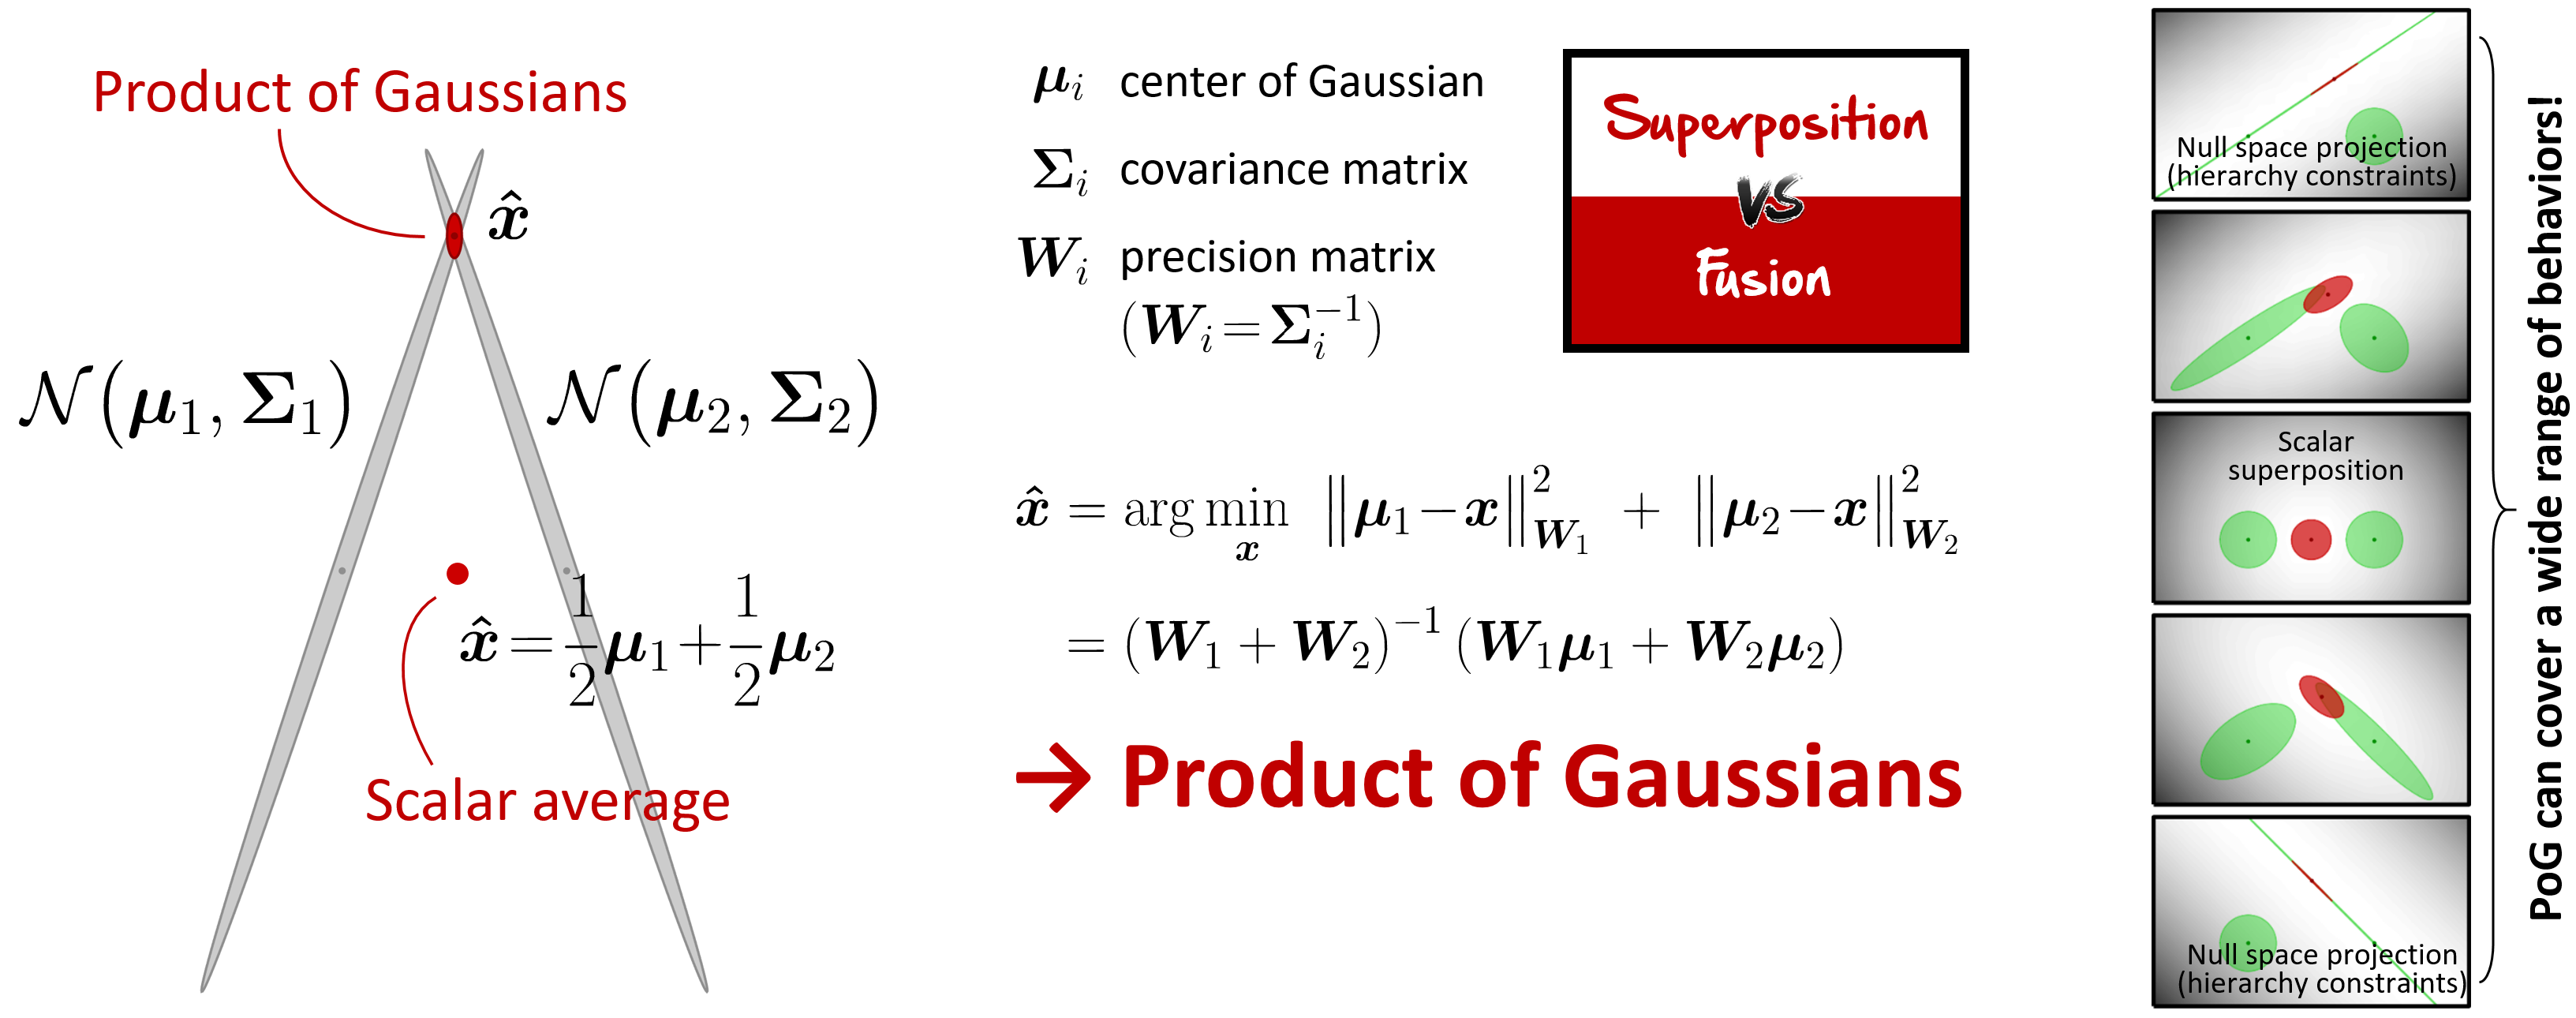
\includegraphics[width=.8\columnwidth]{images/PoG01.png}
\caption{\footnotesize
Quadratic costs minimization as a product of Gaussians (PoG).
}
\label{fig:PoG}
\end{figure}

Figure \ref{fig:PoG} shows an illustration for 2 Gaussians in a 2-dimensional space. It also shows that when one of the Gaussians is singular, the product corresponds to a projection operation, that we for example find in nullspace projections to solve prioritized tasks in robotics. 

%The solution of a cost composed of quadratic terms of the form 
%\begin{align}
%	\bm{\hat{\mu}} &= \arg\min_{\bm{x}} \sum_{k=1}^K {\big\|\bm{x} - \bm{\mu}_k\big\|}^2_{\bm{\Sigma}_k^{-1}} \\
%	&= \arg\min_{\bm{x}} \sum_{k=1}^K {(\bm{x} - \bm{\mu}_k)}^\trsp \bm{\Sigma}_k^{-1} (\bm{x} - \bm{\mu}_k)
%	\label{eq:quadObj}
%\end{align}
%can be computed analytically. It corresponds to the product of Gaussians $\prod_{k=1}^K\mathcal{N}(\bm{\mu}_k,\bm{\Sigma}_k)$, with centers $\bm{\mu}_k$ and covariance matrices $\bm{\Sigma}_k$. The Gaussian $\mathcal{N}(\bm{\hat{\mu}},\bm{\hat{\Sigma}})$ resulting from this product has parameters
%\begin{align*}
%	\bm{\hat{\mu}} &= {\left(\sum_{k=1}^K \bm{\Sigma}_k^{-1} \right)}^{\!-1} \left(\sum_{k=1}^K\bm{\Sigma}_k^{-1} \bm{\mu}_k \right) \\
%	 &= {\left(\sum_{k=1}^K \bm{\Gamma}_k\right)}^{\!-1} \left(\sum_{k=1}^K\bm{\Gamma}_k \bm{\mu}_k \right), \\
%	\bm{\hat{\Sigma}} &= {\left(\sum_{k=1}^K \bm{\Sigma}_k^{-1} \right)}^{\!-1} \\
%	&= {\left(\sum_{k=1}^K \bm{\Gamma}_k\right)}^{\!-1},
%\end{align*}
%which can be computed with covariance matrices $\bm{\Sigma}_k$ or precision matrices $\bm{\Gamma}_k=\bm{\Sigma}_k^{-1}$. Although equivalent algebraically, one or the other form (or a mix of the two) can be preferred from a numerical perspective.

%Solving an objective function composed of quadratic terms as a product of Gaussians offers a probabilistic perspective by representing the solution in the form of a distribution. 

\newpage
%%%%%%%%%%%%%%%%%%%%%%%%%%%%%%%%%%%%%%%%%%%%%%%%%%%%%%%%%%%%%%%%%%%%%%%%%%%%%%%%%
\section{Newton's method for minimization}\label{sec:Newton}

\begin{wrapfigure}{r}{.28\textwidth}
%\vspace{-20pt}
\centering
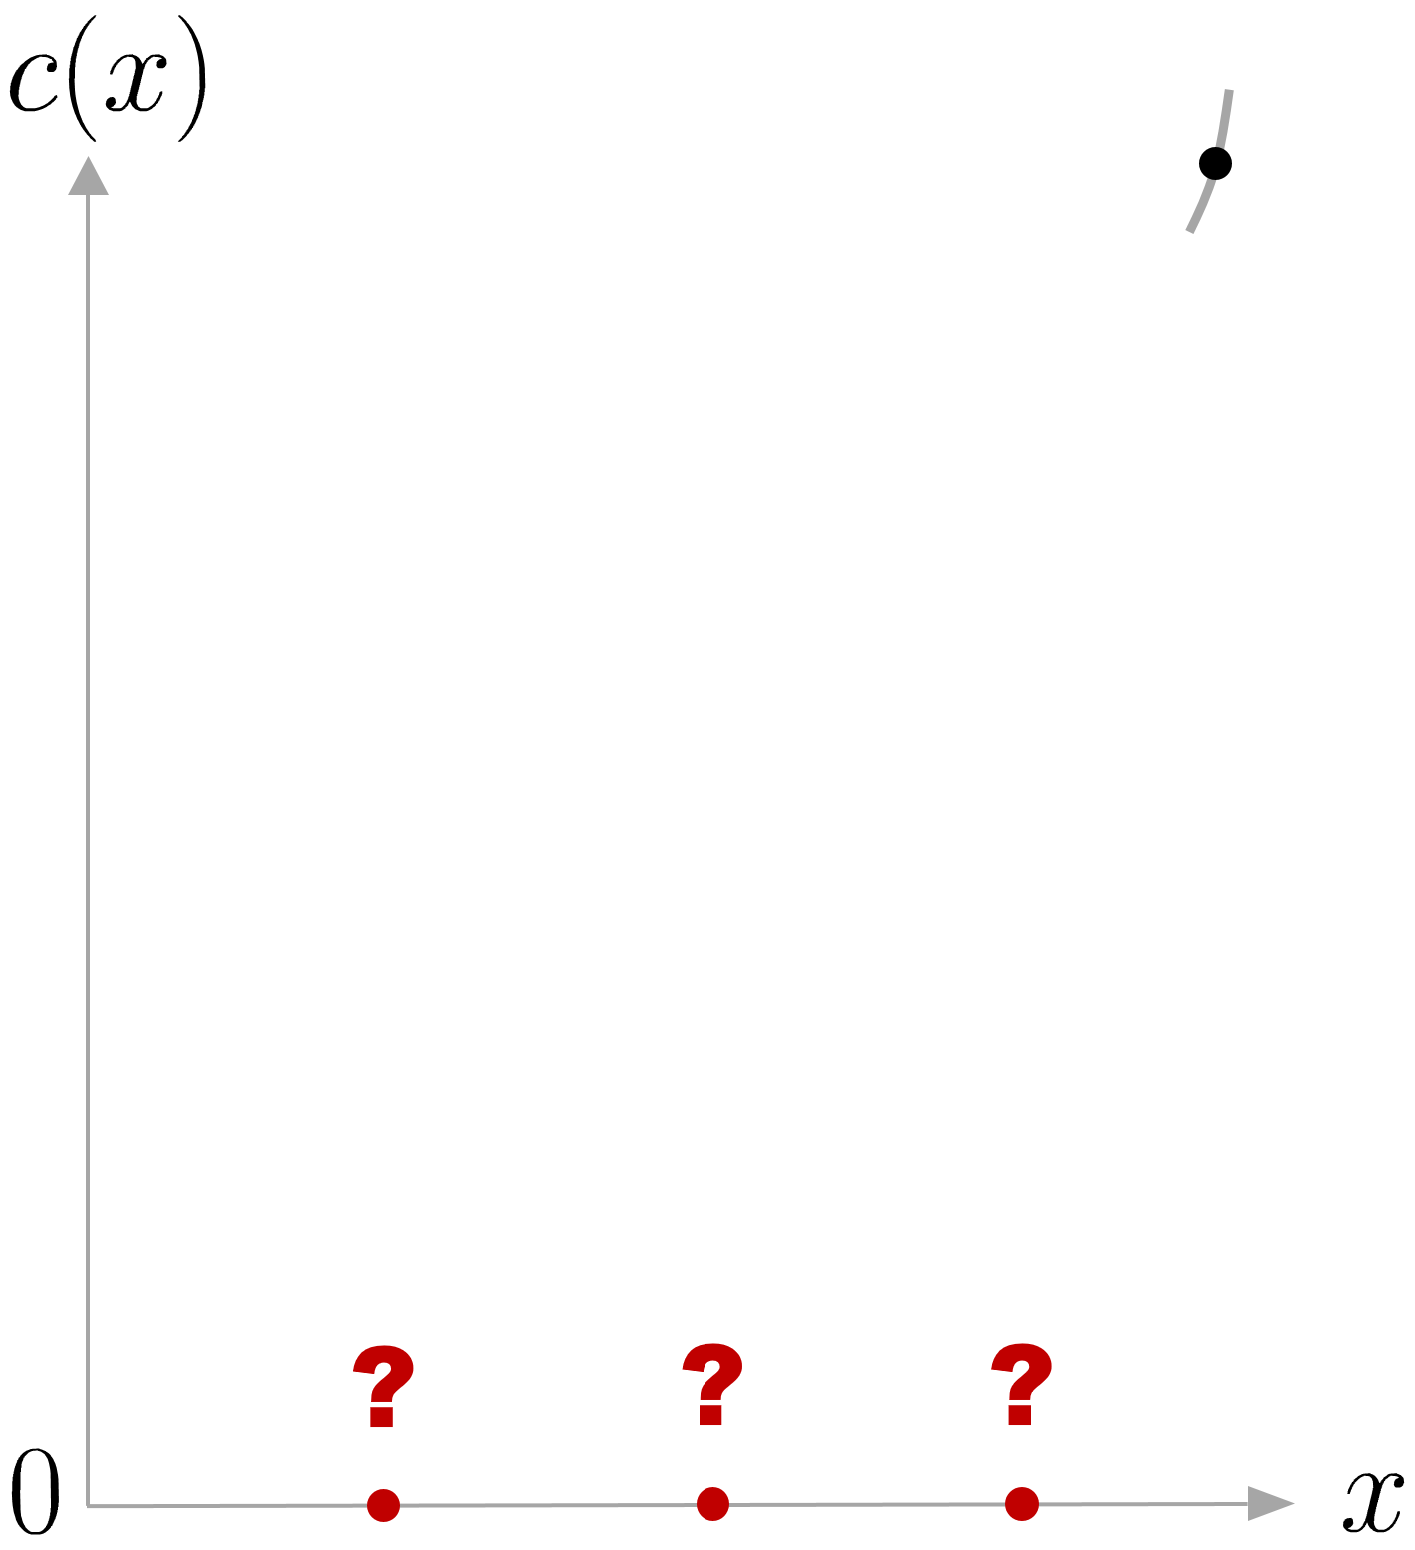
\includegraphics[width=.26\textwidth]{images/NewtonMethod1D_problem01.png}
\caption{\footnotesize
Problem formulation.
}
\label{fig:NewtonProblem}
\vspace{20pt}
\end{wrapfigure}

We would like the find the value of a decision variable $x$ that would give us a cost $c(x)$ that is a small as possible, see Figure \ref{fig:NewtonProblem}. Imagine that we start from an initial guess $x_1$ and that can observe the behavior of this cost function within a very small region around our initial guess. Now let's assume that we can make several consecutive guesses that will each time provide us with similar local information about the behavior of the cost around the points that we guessed. From this information, what point would you select as second guess (see question marks in the figure), based on the information that you obtained from the first guess? There were two relevant information in the small portion of curve that we can observe in the figure to make a smart choice. First, the trend of the curve indicates that the cost seems to decrease if we move on the left side, and increase if we move on the right side. Namely, the slope $c'(x_1)$ of the function $c(x)$ at point $x_1$ is positive. Second, we can observe that the portion of the curve has some curvature that can be also be informative about the way the trend of the curve $c(x)$ will change by moving to the left or to the right. Namely, how much the slope $c'(x_1)$ will change, corresponding to an acceleration $c''(x_1)$ around our first guess $x_1$. This is informative to estimate how much we should move to the left of the first guess to wisely select a second guess. \newline

\begin{wrapfigure}{r}{.48\textwidth}
%\vspace{-20pt}
\centering
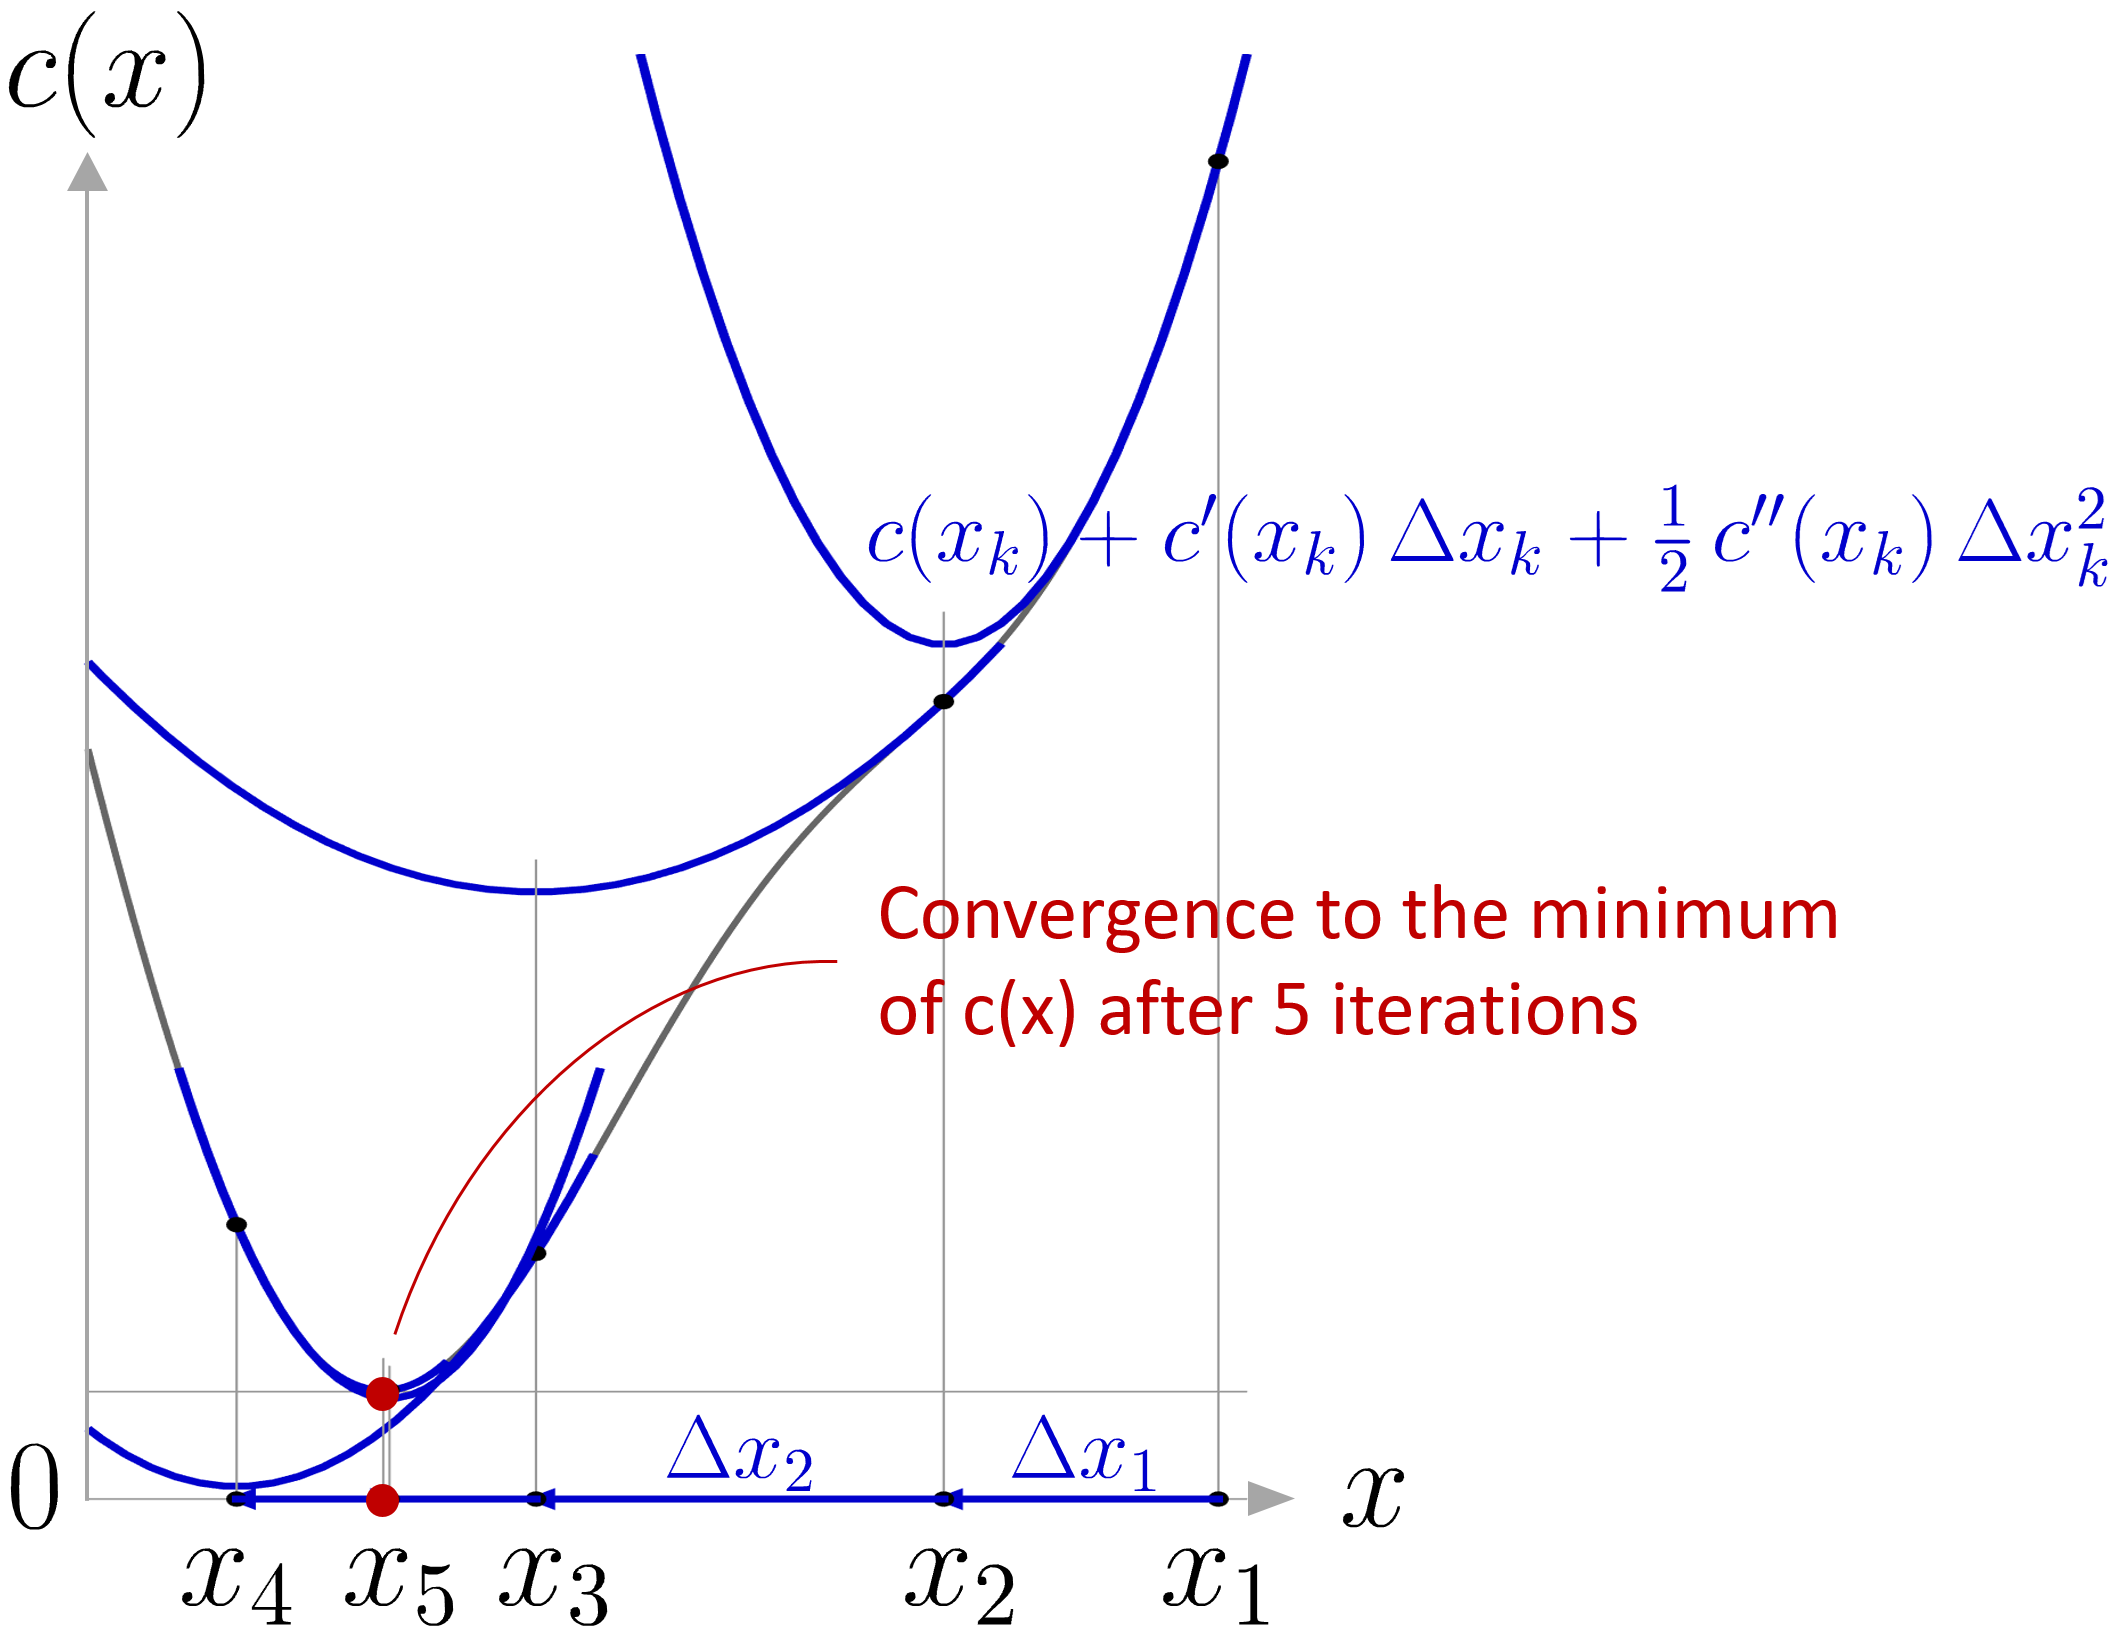
\includegraphics[width=.42\textwidth]{images/NewtonMethod1D01.png}
\caption{\footnotesize
Newton's method for minimization, starting from an initial estimate $x_1$ and converging to a local minimum (red point) after 5 iterations.
}
\label{fig:Newton}
\end{wrapfigure}

Now that we have this intuition, we can move to a more formal problem formulation. Newton's method attempts to solve $\min_x c(x)$ or $\max_x c(x)$ from an initial guess $x_1$ by using a sequence of \textbf{second-order Taylor approximations} of $c(x)$ around the iterates, see Fig.~\ref{fig:Newton}. 

The second-order Taylor expansion around the point $x_k$ can be expressed as
\begin{equation}
	c(x_k\!+\!\Delta x_k) \approx c(x_k) + c'(x_k) \; \Delta x_k + \frac{1}{2} c''(x_k) \; \Delta x_k^2 ,
	\label{eq:Taylor_1D}
\end{equation}
where $c'(x_k)$ and $c''(x_k)$ are the first and second derivatives at point $x_k$.

We are interested in solving minimization problems with this approximation. If the second derivative $c''(x_k)$ is positive, the quadratic approximation is a convex function of $\Delta x_k$, and its minimum can be found by setting the derivative to zero.

\newpage

\begin{wrapfigure}{r}{.28\textwidth}
\vspace{-20pt}
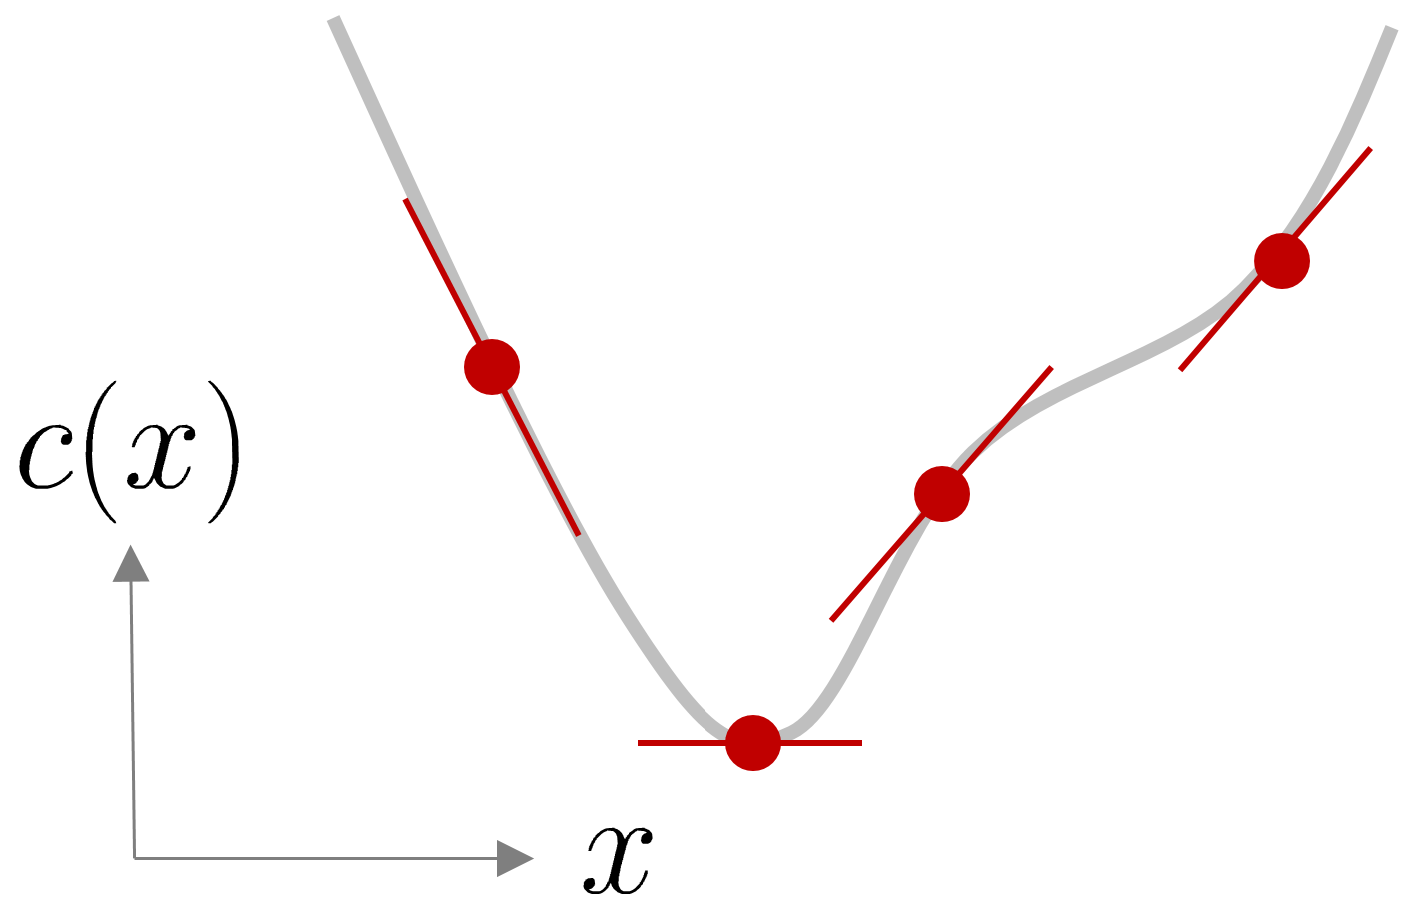
\includegraphics[width=.26\textwidth]{images/optim_principle01.png}
\caption{\footnotesize
Finding local optima by localizing the points whose derivatives are zero (horizontal slopes).
}
\label{fig:optimPrinciple}
\end{wrapfigure}

To find the local optima of a function, we can localize the points whose derivatives are zero, see Figure \ref{fig:optimPrinciple} for an illustration.

Thus, by differentiating \eqref{eq:Taylor_1D} w.r.t.\ $\Delta x_k$ and equating to zero, we obtain 
\begin{equation*}
	c'(x_k) + c''(x_k) \, \Delta x_k = 0,
\end{equation*}
meaning that the minimum is given by
\begin{equation*}
	\Delta\hat{x}_k = - \frac{c'(x_k)}{c''(x_k)}
\end{equation*} 
which corresponds to the offset to apply to $x_k$ to minimize the second-order polynomial approximation of the cost at this point.

\begin{wrapfigure}{r}{.28\textwidth}
%\vspace{-20pt}
\centering
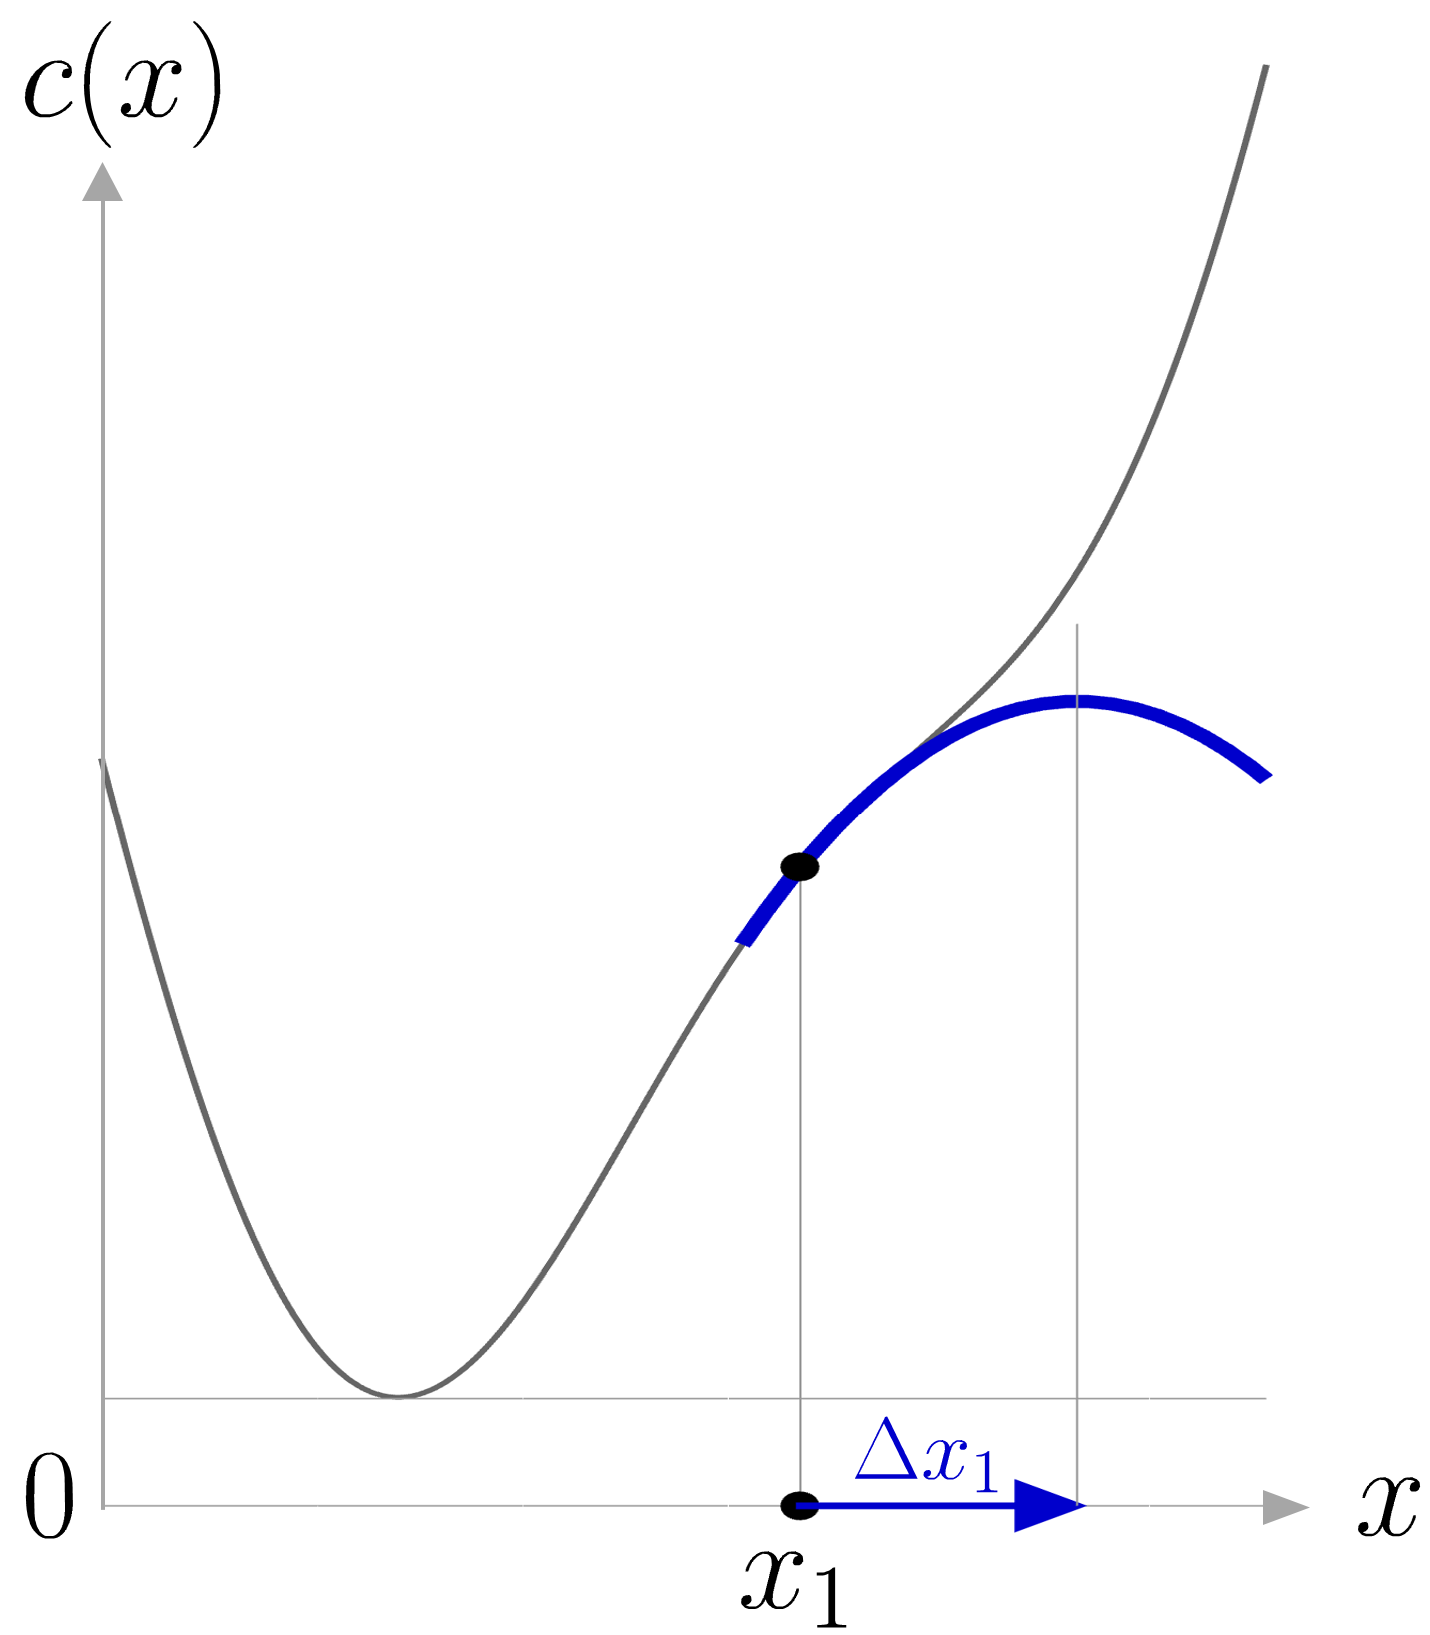
\includegraphics[width=.26\textwidth]{images/NewtonMethod_negativeHessian01.png}
\caption{\footnotesize
Newton update that would be achieved when the second derivative is negative.
}
\label{fig:NewtonNegativeHessian}
%\vspace{-20pt}
\end{wrapfigure}

It is important that $c''(x_k)$ is positive if we want to find local minima, see Figure \ref{fig:NewtonNegativeHessian} for an illustration. 


By starting from an initial estimate $x_1$ and by recursively refining the current estimate by computing the offset that would minimize the polynomial approximation of the cost at the current estimate, we obtain at each iteration $k$ the recursion
\begin{equation}
	x_{k+1} = x_k - \frac{c'(x_k)}{c''(x_k)}.
	\label{eq:Taylor_1D_update}
\end{equation}

The geometric interpretation of Newton's method is that at each iteration, it amounts to the fitting of a paraboloid to the surface of $c(x)$ at $x_k$, having the same slopes and curvature as the surface at that point, and then proceeding to the maximum or minimum of that paraboloid. Note that if $c(x)$ is a quadratic function, then the exact extremum is found in one step, which corresponds to the resolution of a least-squares problem. 
%Note also that Newton's method is often modified to include a step size (e.g., estimated with line search).


%%%%%%%%%%%%%%%%%%%%%%%%%%%%%%%%%%%%%%
\subsubsection*{Multidimensional case}

\begin{wrapfigure}{r}{.48\textwidth}
%\vspace{-20pt}
\centering
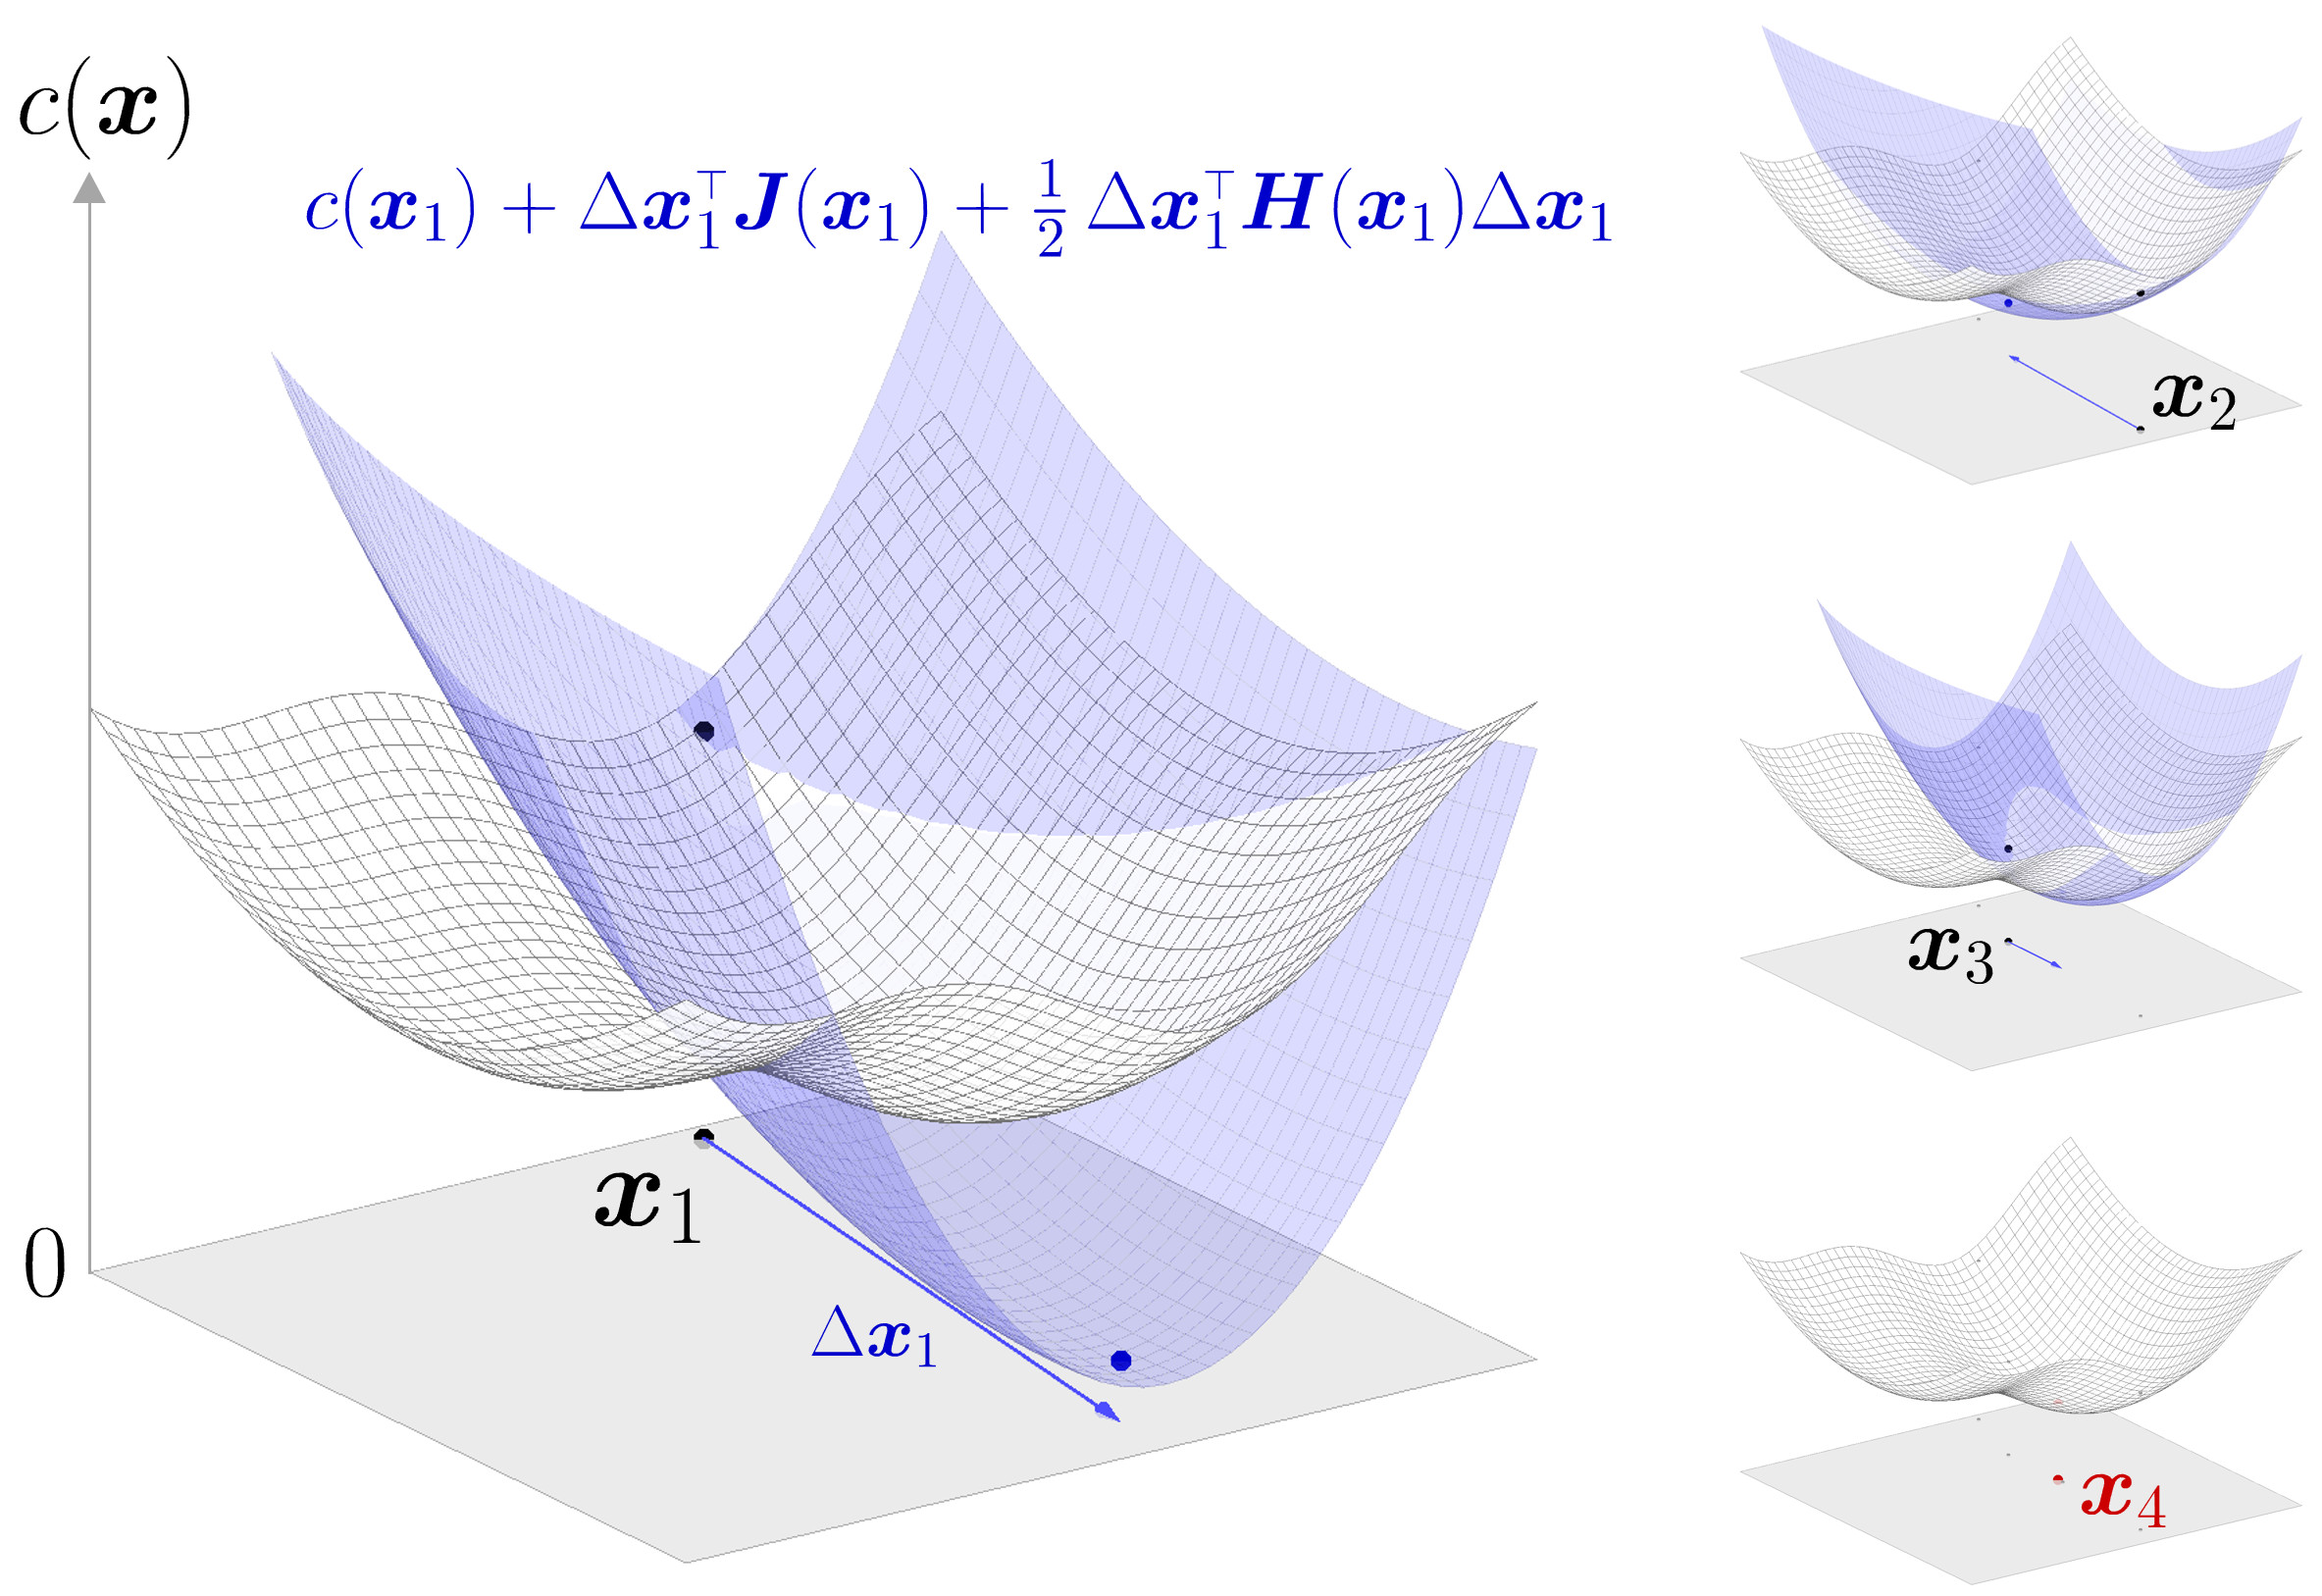
\includegraphics[width=.46\textwidth]{images/NewtonMethod2D01.jpg}
\caption{\footnotesize
Newton's method for minimization with 2D decision variables.
}
\label{fig:Newton2D}
%\vspace{-20pt}
\end{wrapfigure}

For functions that depend on multiple variables stored as multidimensional vectors $\bm{x}$, the cost function $c(\bm{x})$ can similarly be approximated by a second-order Taylor expansion around the point $\bm{x}_k$ with
\begin{equation}
	c(\bm{x}_k\!+\!\Delta\bm{x}_k) \approx c(\bm{x}_k) + \Delta\bm{x}_k^\trsp \, \frac{\partial c}{\partial\bm{x}}\Big|_{\bm{x}_k} +
	\frac{1}{2}\Delta\bm{x}_k^\trsp \, \frac{\partial^2c}{\partial\bm{x}^2}\Big|_{\bm{x}_k} \Delta\bm{x}_k,
	\label{eq:Taylor_nD}
\end{equation}
which can also be rewritten in augmented vector form as
\begin{equation*}
	c(\bm{x}_k\!+\!\Delta\bm{x}_k) \approx c(\bm{x}_k) + 
	\frac{1}{2}
	\begin{bmatrix}
	1 \\ \Delta\bm{x}_k
	\end{bmatrix}^{\!\trsp}
	\begin{bmatrix}
	0 & \bm{g}_{\bm{x}}^\trsp \\
	\bm{g}_{\bm{x}} & \bm{H}_{\bm{x}\bm{x}} 
	\end{bmatrix}
	\begin{bmatrix}
	1 \\ \Delta\bm{x}_k
	\end{bmatrix},
\end{equation*}
with gradient vector
\begin{equation}
	\bm{g}(\bm{x}_k) = \frac{\partial c}{\partial\bm{x}}\Big|_{\bm{x}_k},
	\label{eq:Taylor_grad}
\end{equation}
and Hessian matrix
\begin{equation}
	\bm{H}(\bm{x}_k) = \frac{\partial^2c}{\partial\bm{x}^2}\Big|_{\bm{x}_k}.
	\label{eq:Taylor_Hess}
\end{equation}

We are interested in solving minimization problems with this approximation. If the Hessian matrix $\bm{H}(\bm{x}_k)$ is positive definite, the quadratic approximation is a convex function of $\Delta\bm{x}_k$, and its minimum can be found by setting the derivatives to zero, see Figure \ref{fig:Newton2D}.

By differentiating \eqref{eq:Taylor_nD} w.r.t.\ $\Delta\bm{x}_k$ and equation to zero, we obtain that
\begin{equation*}
	\Delta\bm{\hat{x}}_k = - {\bm{H}(\bm{x}_k)}^{-1} \, \bm{g}(\bm{x}_k),
\end{equation*} 
is the offset to apply to $\bm{x}_k$ to minimize the second-order polynomial approximation of the cost at this point.

By starting from an initial estimate $\bm{x}_1$ and by recursively refining the current estimate by computing the offset that would minimize the polynomial approximation of the cost at the current estimate, we obtain at each iteration $k$ the recursion
\begin{equation}
	\bm{x}_{k+1} = \bm{x}_k - {\bm{H}(\bm{x}_k)}^{-1} \, \bm{g}(\bm{x}_k).
	\label{eq:Taylor_nD_update}
\end{equation}


%%%%%%%%%%%%%%%%%%%%%%%%%%%%%%%%%%%%%%
\subsection{Gauss--Newton algorithm}\label{sec:GaussNewton}
%https://en.wikipedia.org/wiki/Gauss%E2%80%93Newton_algorithm (section Derivation from Newton's method)
%http://homepages.laas.fr/nmansard/teach/robotics2015/textbook_draft.pdf

The Gauss--Newton algorithm is a special case of Newton's method in which the cost is quadratic (sum of squared function values), with $c(\bm{x})=\sum_{i=1}^R r_i^2(\bm{x})=\bm{r}^\trsp\bm{r}=\|r\|^2$, where $\bm{r}$ are residual vectors. We neglect in this case the second-order derivative terms of the Hessian. The gradient and Hessian can in this case be computed with 
\begin{equation*}
	\bm{g} = 2 \bm{J}_{\bm{r}}^\trsp \bm{r} ,\quad 
	\bm{H} \approx 2 \bm{J}_{\bm{r}}^\trsp \bm{J}_{\bm{r}},
\end{equation*}
where $\bm{J}_{\bm{r}}\in\mathbb{R}^{R\times D}$ is the Jacobian matrix of $\bm{r}\in\mathbb{R}^R$. This definition of the Hessian matrix makes it positive definite, which is useful to solve minimization problems as for well conditioned Jacobian matrices, we do not need to verify the positive definiteness of the Hessian matrix at each iteration.

The update rule in \eqref{eq:Taylor_nD_update} then becomes
\begin{align}
	\bm{x}_{k+1} &= \bm{x}_k - {\big(\bm{J}_{\bm{r}}^\trsp(\bm{x}_k) \bm{J}_{\bm{r}}(\bm{x}_k)\big)}^{-1} \, 
	\bm{J}_{\bm{r}}^\trsp(\bm{x}_k) \, \bm{r}(\bm{x}_k) \\
	&= \bm{x}_k - \bm{J}_{\bm{r}}^\psin(\bm{x}_k) \, \bm{r}(\bm{x}_k),
	\label{eq:GaussNewtonUpdate}
\end{align}
where $\bm{J}_{\bm{r}}^\psin$ denotes the pseudoinverse of $\bm{J}_{\bm{r}}$.

The Gauss--Newton algorithm is the workhorse of many robotics problems, including inverse kinematics and optimal control, as we will see in the next sections.


%%%%%%%%%%%%%%%%%%%%%%%%%%%%%%%%%%%%%%
\subsection{Least squares}\label{sec:LS}

When the cost $c(\bm{x})$ is a quadratic function w.r.t.\ $\bm{x}$, the optimization problem can be solved directly, without requiring iterative steps. Indeed, for any matrix $\bm{A}$ and vector $\bm{b}$, we can see that if
\begin{equation*}
	c(\bm{x}) = (\bm{A}\bm{x}-\bm{b})^\trsp (\bm{A}\bm{x}-\bm{b}),
\end{equation*}
derivating $c(\bm{x})$ w.r.t.\ $\bm{x}$ and equating to zero yields
\begin{equation*}
	\bm{A}\bm{x} - \bm{b} = \bm{0} 
	\iff \bm{x} = \bm{A}^\psin\bm{b},
\end{equation*}
which corresponds to the standard analytic least squares estimate. We will see later in the inverse kinematics section that for the complete solution can also include a nullspace structure. 


%%%%%%%%%%%%%%%%%%%%%%%%%%%%%%%%%%%%%%
\subsection{Least squares with constraints}\label{sec:LSconstraints}

A constrained minimization problem of the form
\begin{equation}
	\min_{\bm{x}} \; (\bm{A}\bm{x}-\bm{b})^\trsp (\bm{A}\bm{x}-\bm{b}),
	\quad\text{s.t.}\quad
	\bm{C}\bm{x}=\bm{h},
	\label{eq:LSconstraints} 
\end{equation}
can also be solved analytically by considering a Lagrange multiplier variable $\bm{\lambda}$ allowing us to rewrite the objective as
\begin{equation*}
	\min_{\bm{x},\bm{\lambda}} \; (\bm{A}\bm{x}-\bm{b})^\trsp (\bm{A}\bm{x}-\bm{b})
	+ \bm{\lambda}^\trsp (\bm{C}\bm{x}-\bm{h}). 
\end{equation*}

Differentiating with respect to $\bm{x}$ and $\bm{\lambda}$ and equating to zero yields
\begin{equation*}
	\bm{A}^\trsp(\bm{A}\bm{x} - \bm{b}) + \bm{C}^\trsp \bm{\lambda} = \bm{0},
	\quad
	\bm{C}\bm{x} - \bm{h} = \bm{0},
\end{equation*}
which can rewritten in matrix form as
\begin{equation*}
	\begin{bmatrix} \bm{A}^\trsp\!\bm{A} & \bm{C}^\trsp \\ \bm{C} & \bm{0} \end{bmatrix} 	
	\begin{bmatrix} \bm{x} \\ \bm{\lambda} \end{bmatrix}
	=
	\begin{bmatrix} \bm{A}^\trsp\bm{b} \\ \bm{h} \end{bmatrix}.
\end{equation*}

With this augmented state representation, we can then see that 
\begin{equation*}
	\begin{bmatrix} \bm{x} \\ \bm{\lambda} \end{bmatrix} =
	\begin{bmatrix} \bm{A}^\trsp\!\bm{A} & \bm{C}^\trsp \\ \bm{C} & \bm{0} \end{bmatrix}^{-1} \begin{bmatrix} \bm{A}^\trsp\bm{b} \\ \bm{h} \end{bmatrix} 
\end{equation*}
minimizes the constrained cost. The first part of this augmented state then gives us the solution of \eqref{eq:LSconstraints}.


\newpage
%%%%%%%%%%%%%%%%%%%%%%%%%%%%%%%%%%%%%%%%%%%%%%%%%%%%%%%%%%%%%%%%%%%%%%%%%%%%%%%%%
\section{Forward kinematics (FK) for a planar robot manipulator}\label{sec:FK}
\begin{flushright}
\filename{IK.*}
\end{flushright}

%\begin{figure}
%\centering
%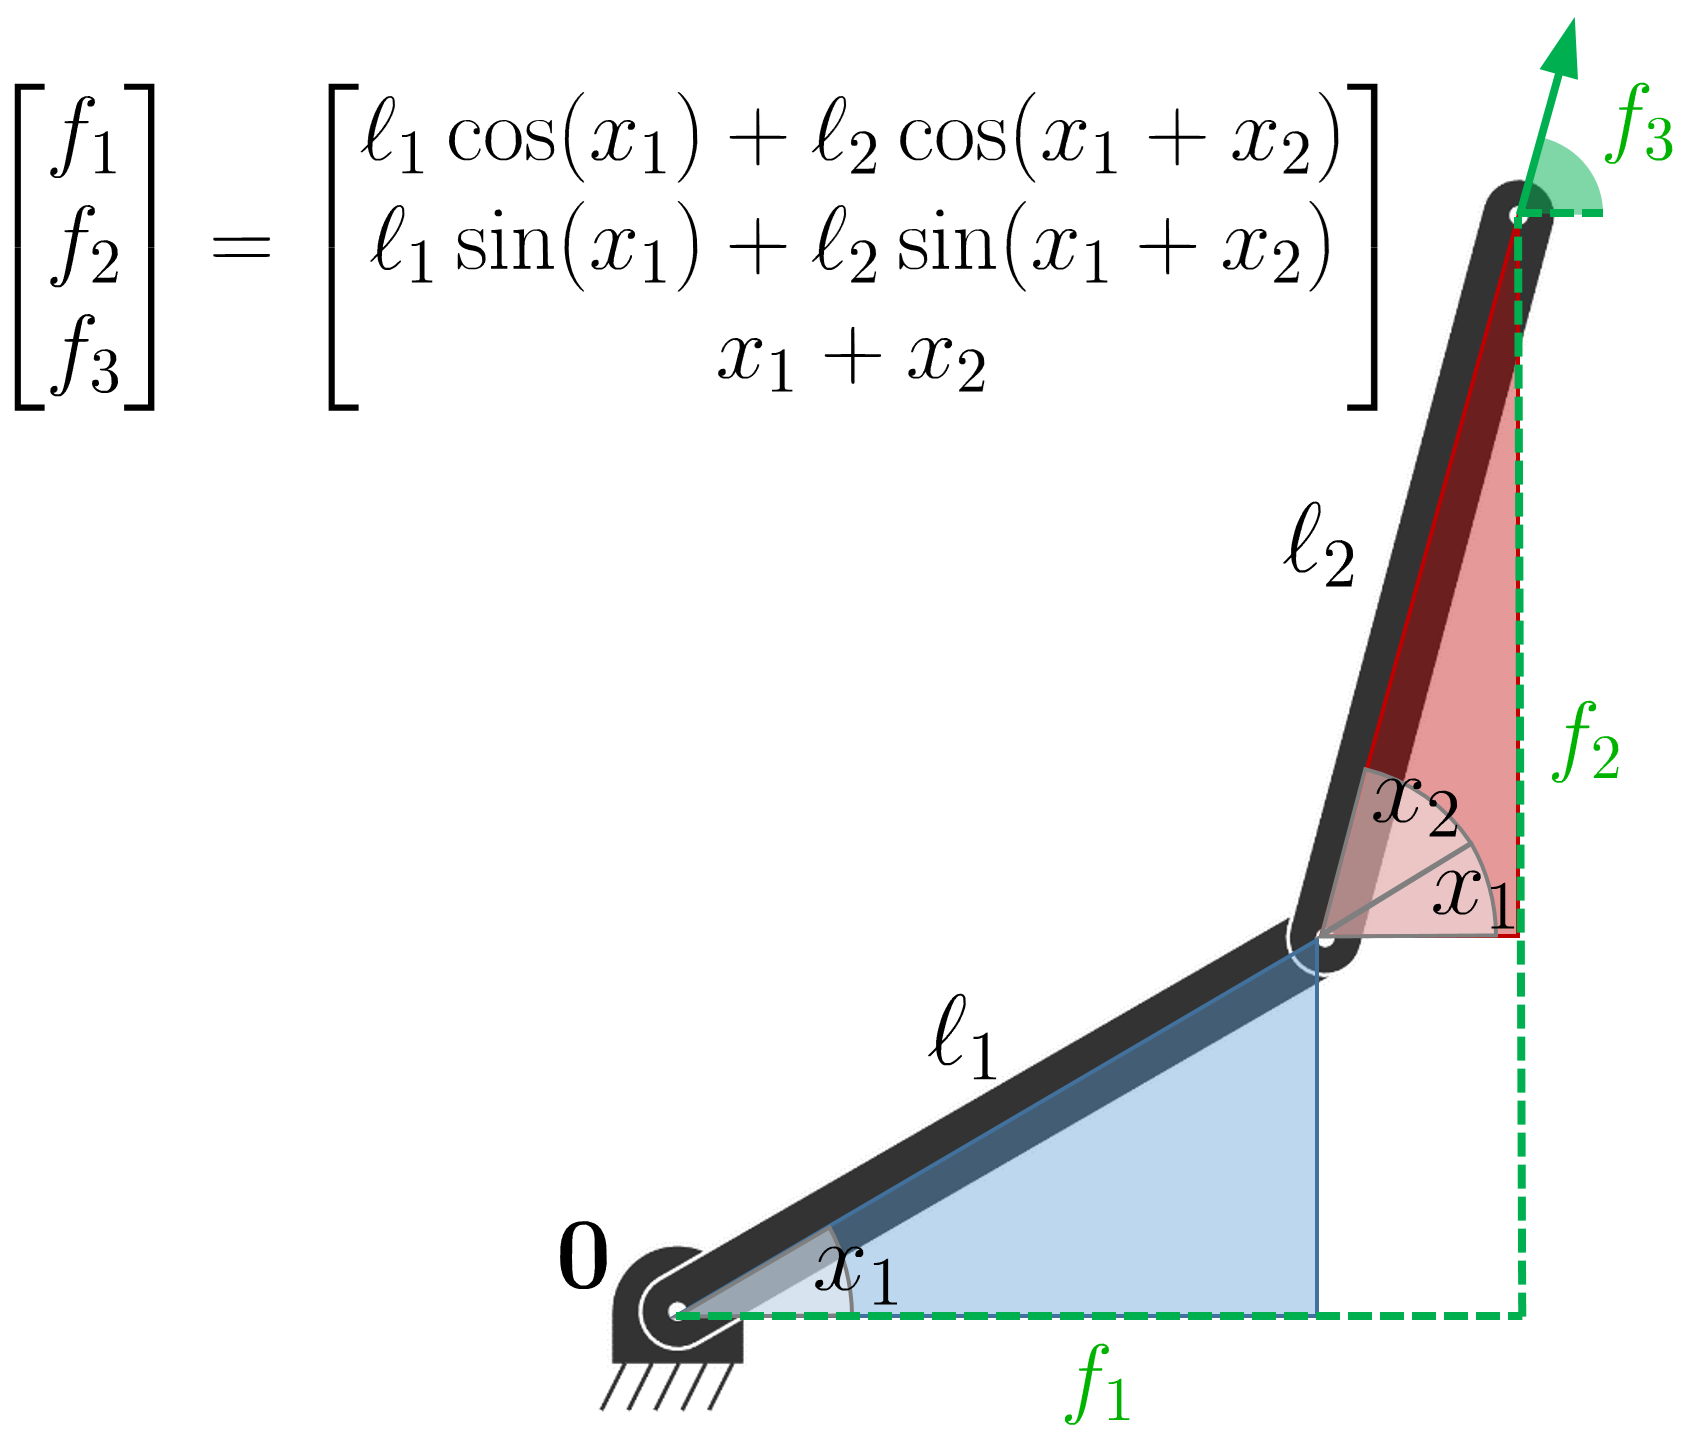
\includegraphics[width=.6\columnwidth]{images/f_ee01.png}
%\caption{\footnotesize
%Forward kinematics for a planar robot with two links.
%}
%\label{fig:FK}
%\end{figure}

\begin{wrapfigure}{r}{.36\textwidth}
%\vspace{-20pt}
\centering
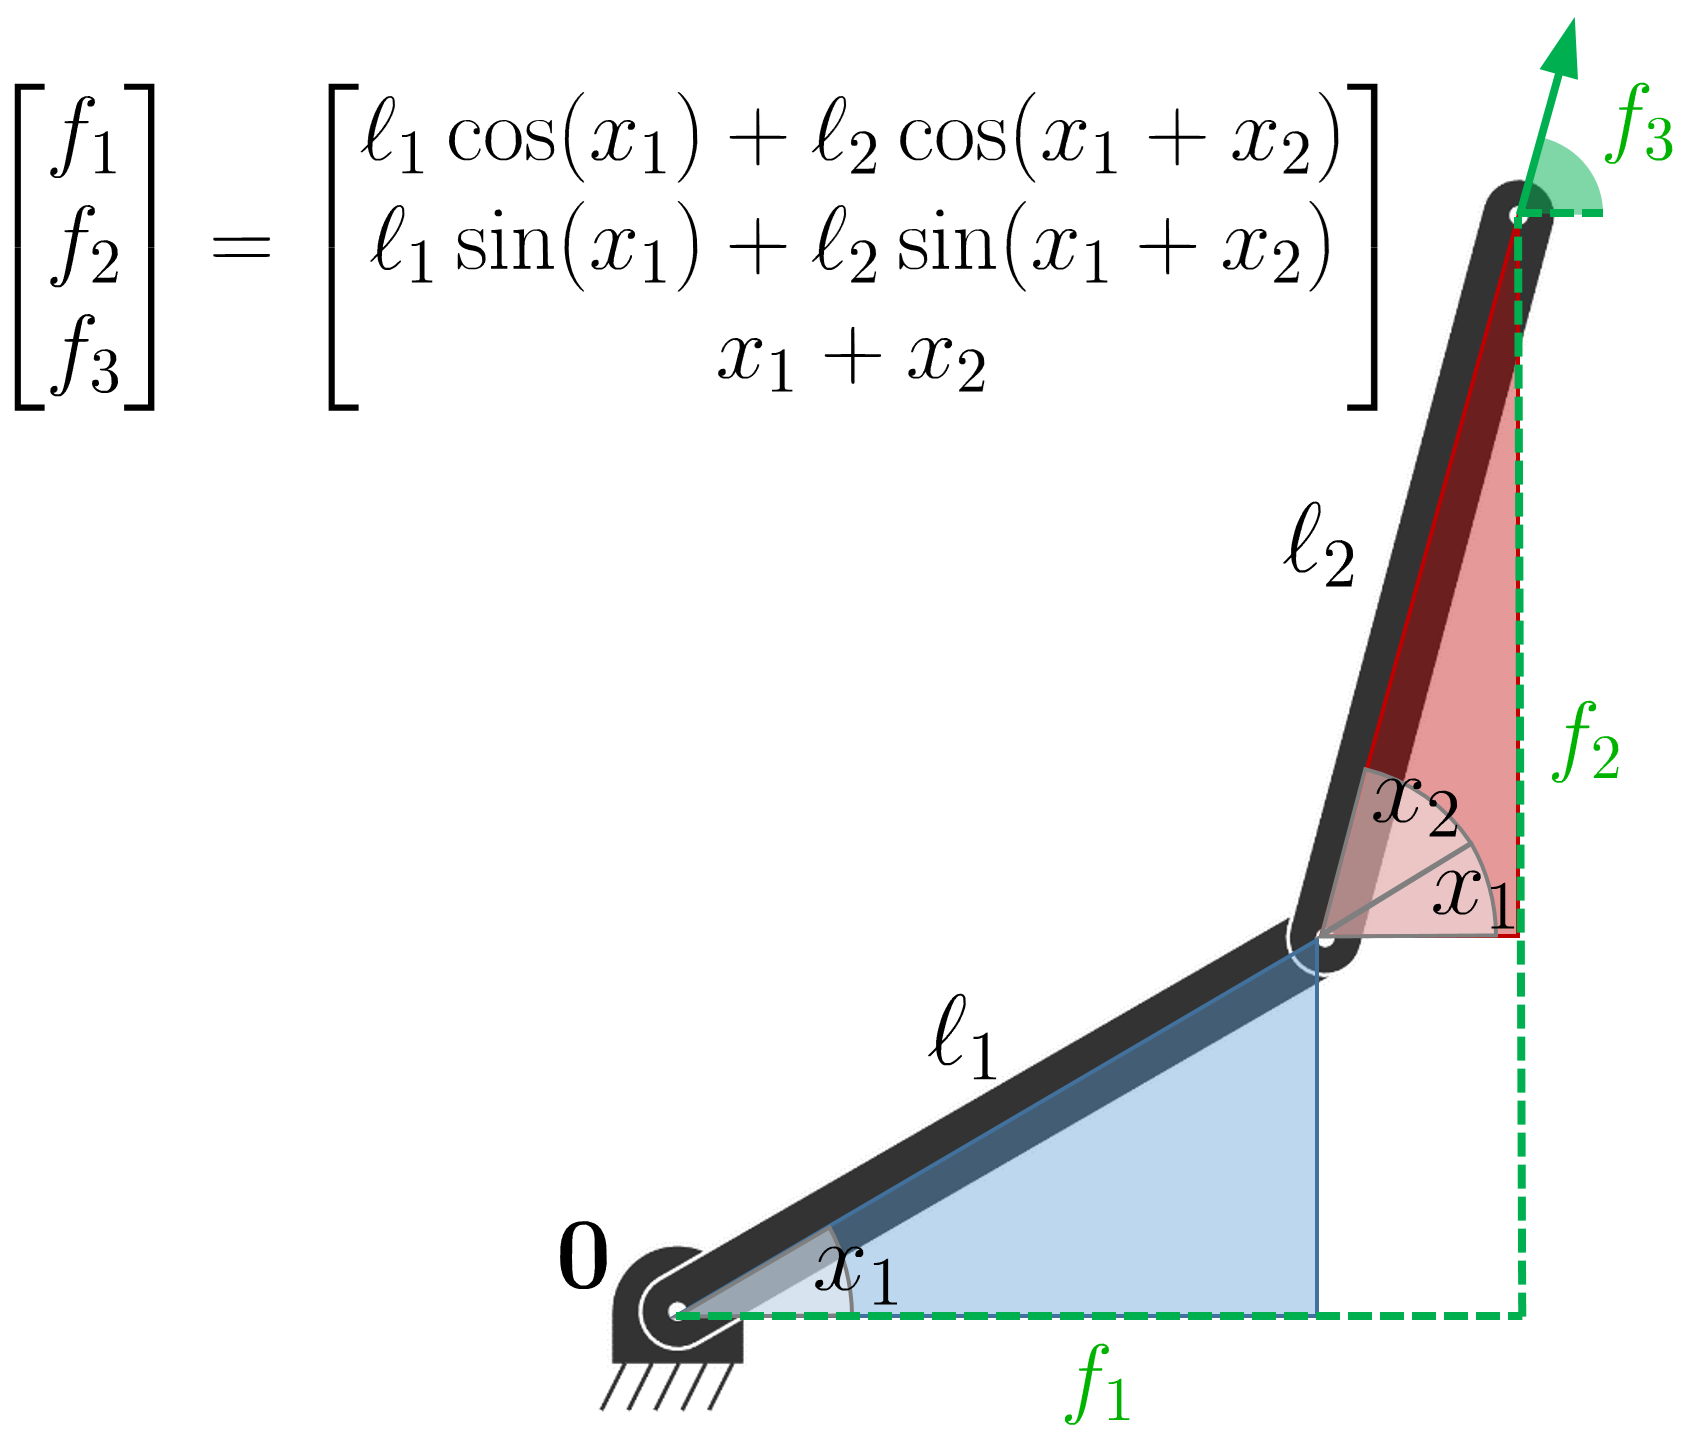
\includegraphics[width=.34\textwidth]{images/f_ee01.png}
\caption{\footnotesize
Forward kinematics for a planar robot with two links.
}
\label{fig:FK}
%\vspace{-20pt}
\end{wrapfigure}

The \emph{forward kinematics} (FK) function of a planar robot manipulator is defined as
\begin{align*}
	\bm{f} &= \begin{bmatrix} \bm{\ell}^\trsp \cos(\bm{L}\bm{x}) \\ \bm{\ell}^\trsp \sin(\bm{L}\bm{x}) \\ \bm{1}^\trsp \bm{x} \end{bmatrix} \\
	&= \begin{bmatrix} 
	\ell_1 \!\cos(x_1) \!+\! \ell_2 \!\cos(x_1\!+\!x_2) \!+\! \ell_3 \!\cos(x_1\!+\!x_2\!+\!x_3) \!+\! \ldots\\ 
	\ell_1 \sin(x_1) \!+\! \ell_2 \!\sin(x_1\!+\!x_2) \!+\! \ell_3 \!\sin(x_1\!+\!x_2\!+\!x_3) \!+\! \ldots\\ 
	x_1+x_2+x_3+\ldots 
	\end{bmatrix} \!\!,
\end{align*}
%	T = tril(ones(size(x,1)));
%	f = [model.l * cos(T * x); ...
%		 model.l * sin(T * x); ...
%		 mod(sum(x,1)+pi, 2*pi) - pi];
with $\bm{x}$ the state of the robot (joint angles), $\bm{f}$ the position of the robot end-effector, $\bm{\ell}\,$ a vector of robot links lengths, $\bm{L}$ a lower triangular matrix with unit elements, and $\bm{1}$ a vector of unit elements, see Fig.~\ref{fig:FK}.

The position and orientation of all articulations can similarly be computed with the forward kinematics function
\begin{align}
	\bm{\tilde{f}} &= {\Big[ \bm{L}\; \diag(\bm{\ell}) \cos(\bm{L}\bm{x}) ,\quad \bm{L}\; \diag(\bm{\ell}) \sin(\bm{L}\bm{x}) ,\quad \bm{L} \bm{x} \Big]}^\trsp 
	\nonumber\\
	&= \begin{bmatrix} 
	\tilde{f}_{1,1} & \tilde{f}_{1,2} & \tilde{f}_{1,3} & \ldots\\ 
	\tilde{f}_{2,1} & \tilde{f}_{2,2} & \tilde{f}_{2,3} & \ldots\\ 
	\tilde{f}_{3,1} & \tilde{f}_{3,2} & \tilde{f}_{3,3} & \ldots\\ 
	\end{bmatrix} \!\!,
	\label{eq:FKall}
\end{align} 
\begin{alignat*}{3}
	& \tilde{f}_{1,1} = \ell_1 \!\cos(x_1),\quad &&
	\tilde{f}_{1,2} = \ell_1 \!\cos(x_1) \!+\! \ell_2 \!\cos(x_1\!+\!x_2),\quad &&
	\tilde{f}_{1,3} = \ell_1 \!\cos(x_1) \!+\! \ell_2 \!\cos(x_1\!+\!x_2) \!+\! \ell_3 \!\cos(x_1\!+\!x_2\!+\!x_3),\\ 
\text{with}\quad 
	& \tilde{f}_{2,1} = \ell_1 \sin(x_1), &&
	\tilde{f}_{2,2} = \ell_1 \sin(x_1) \!+\! \ell_2 \!\sin(x_1\!+\!x_2), &&
	\tilde{f}_{2,3} = \ell_1 \sin(x_1) \!+\! \ell_2 \!\sin(x_1\!+\!x_2) \!+\! \ell_3 \!\sin(x_1\!+\!x_2\!+\!x_3), \quad\ldots\\ 
	& \tilde{f}_{3,1} = x_1, &&
	\tilde{f}_{3,2} = x_1 + x_2, &&
	\tilde{f}_{3,3} = x_1 + x_2 + x_3.
\end{alignat*}

%\begin{align*}
%	\tilde{f}_{1,1} &= \ell_1 \!\cos(x_1),\\ 
%	\tilde{f}_{2,1} &= \ell_1 \sin(x_1),\\ 
%	\tilde{f}_{3,1} &= x_1,\\[2mm]
%	
%	\tilde{f}_{1,2} &= \ell_1 \!\cos(x_1) \!+\! \ell_2 \!\cos(x_1\!+\!x_2),\\ 
%	\tilde{f}_{2,2} &= \ell_1 \sin(x_1) \!+\! \ell_2 \!\sin(x_1\!+\!x_2),\\ 
%	\tilde{f}_{3,2} &= x_1 + x_2,\\[2mm]
%	
%	\tilde{f}_{1,3} &= \ell_1 \!\cos(x_1) \!+\! \ell_2 \!\cos(x_1\!+\!x_2) \!+\! \ell_3 \!\cos(x_1\!+\!x_2\!+\!x_3),\\ 
%	\tilde{f}_{2,3} &= \ell_1 \sin(x_1) \!+\! \ell_2 \!\sin(x_1\!+\!x_2) \!+\! \ell_3 \!\sin(x_1\!+\!x_2\!+\!x_3),\\ 
%	\tilde{f}_{3,3} &= x_1 + x_2 + x_3,\\
%	\vdots &
%\end{align*}

In Python, this can be coded for the end-effector position part as
\begin{lstlisting}[language=Python,linewidth=\textwidth]
D = 3 #State space dimension (joint angles) 
x = np.ones(D) * np.pi / D #Robot pose
l = np.array([2, 2, 1]) #Links lengths
L = np.tril(np.ones([D,D])) #Transformation matrix
f = np.array([L @ np.diag(l) @ np.cos(L @ x), L @ np.diag(l) @ np.sin(L @ x)]) #Forward kinematics
\end{lstlisting}


\newpage

%%%%%%%%%%%%%%%%%%%%%%%%%%%%%%%%%%%%%%%%%%%%%%%%%%%%%%%%%%%%%%%%%%%%%%%%%%%%%%%%%
\section{Inverse kinematics (IK) for a planar robot manipulator}\label{sec:IK}
\begin{flushright}
\filename{IK.*}
\end{flushright}

By differentiating the forward kinematics function, a least norm inverse kinematics solution can be computed with
\begin{equation}
	\bm{\dot{\bm{x}}} = \bm{J}^\psin\!(\bm{x}) \; \bm{\dot{f}},
	\label{eq:IK_LS}
\end{equation}
where the Jacobian $\bm{J}(\bm{x})$ corresponding to the end-effector forward kinematics function $\bm{f}(\bm{x})$ can be computed as (with a simplification for the orientation part by ignoring the manifold aspect)
\begin{align*}
	\bm{J} &= \begin{bmatrix} 
	-\sin(\bm{L}\bm{x})^\trsp \diag(\bm{\ell}) \bm{L} \\ 
	 \cos(\bm{L}\bm{x})^\trsp \diag(\bm{\ell}) \bm{L} \\ 
	 \bm{1}^\trsp \end{bmatrix} \\
	&= \begin{bmatrix} 
	J_{1,1} & J_{1,2} & J_{1,3} & \ldots\\
	J_{2,1} & J_{2,2} & J_{2,3} & \ldots\\
	J_{3,1} & J_{3,2} & J_{3,3} & \ldots\\
	\end{bmatrix} \!\!,
\end{align*}
with
{\scriptsize
\begin{alignat*}{3}
	& J_{1,1} = -\ell_1 \!\sin(x_1) \!-\! \ell_2 \!\sin(x_1\!+\!x_2) \!-\! \ell_3 \!\sin(x_1\!+\!x_2\!+\!x_3) \!-\! \ldots,\quad 
	&& J_{1,2} = -\ell_2 \!\sin(x_1\!+\!x_2) \!-\! \ell_3 \!\sin(x_1\!+\!x_2\!+\!x_3) \!-\! \ldots,\quad 
	&& J_{1,3} = -\ell_3 \!\sin(x_1\!+\!x_2\!+\!x_3) \!-\! \ldots,
	\\
	& J_{2,1} = \ell_1 \!\cos(x_1) \!+\! \ell_2 \!\cos(x_1\!+\!x_2) \!+\! \ell_3 \!\cos(x_1\!+\!x_2\!+\!x_3) \!+\! \ldots, 
	&& J_{2,2} = \ell_2 \!\cos(x_1\!+\!x_2) \!+\! \ell_3 \!\cos(x_1\!+\!x_2\!+\!x_3) \!+\! \ldots, 
	&& J_{2,3} = \ell_3 \!\cos(x_1\!+\!x_2\!+\!x_3) \!+\! \ldots, \quad\ldots
	\\
	& J_{3,1} = 1, 
	&& J_{3,2} = 1, 
	&& J_{3,3} = 1,
\end{alignat*}
}
%with
%\begin{align*}
%	J_{1,1} &= -\ell_1 \!\sin(x_1) \!-\! \ell_2 \!\sin(x_1\!+\!x_2) \!-\! \ell_3 \!\sin(x_1\!+\!x_2\!+\!x_3) \!-\! \ldots,\\
%	J_{2,1} &= \ell_1 \!\cos(x_1) \!+\! \ell_2 \!\cos(x_1\!+\!x_2) \!+\! \ell_3 \!\cos(x_1\!+\!x_2\!+\!x_3) \!+\! \ldots,\\
%	J_{3,1} &= 1,\\[2mm]
%	J_{1,2} &= -\ell_2 \!\sin(x_1\!+\!x_2) \!-\! \ell_3 \!\sin(x_1\!+\!x_2\!+\!x_3) \!-\! \ldots,\\
%	J_{2,2} &= \ell_2 \!\cos(x_1\!+\!x_2) \!+\! \ell_3 \!\cos(x_1\!+\!x_2\!+\!x_3) \!+\! \ldots,\\
%	J_{3,2} &= 1,\\[2mm]
%	J_{1,3} &= -\ell_3 \!\sin(x_1\!+\!x_2\!+\!x_3) \!-\! \ldots,\\
%	J_{2,3} &= \ell_3 \!\cos(x_1\!+\!x_2\!+\!x_3) \!+\! \ldots,\\
%	J_{3,3} &= 1,\\
%	\vdots &
%\end{align*}
%%J = [-sin(T * x)' * T * diag(model.l); ...
%%		  cos(T * x)' * T * diag(model.l); ...
%%		  ones(1, size(x,1))]; %x1,x2,o

In Python, this can be coded for the end-effector position part as
\begin{lstlisting}[language=Python,linewidth=\textwidth]
J = np.array([-np.sin(L @ x).T @ np.diag(l) @ L, np.cos(L @ x).T @ np.diag(l) @ L]) #Jacobian (for end-effector)
\end{lstlisting}

This Jacobian can be used to solve the \emph{inverse kinematics} (IK) problem that consists of finding a robot pose to reach a target with the robot endeffector. The underlying optimization problem consists of minimizing a quadratic cost $c=\|\bm{f}-\bm{\mu}\|^2$, where $\bm{f}$ is the position of the endeffector and $\bm{\mu}$ is a target to reach with this endeffector. An optimization problem with a quadratic cost can be solved iteratively with a Gauss--Newton method, requiring to compute Jacobian pseudoinverses $\bm{J}^\psin$, see Section \ref{sec:GaussNewton} for details.


%%%%%%%%%%%%%%%%%%%%%%%%%%%%%%%%%%%%%%%%%%%%%%%%%%%%%%%%%%%%%%%%%%%%%%%%%%%%%%%%%
\subsection{Numerical estimation of the Jacobian}\label{sec:IKnum}
\begin{flushright}
\filename{IK\_num.*}
\end{flushright}

Section \ref{sec:IK} above presented an analytical solution for the Jacobian. A numerical solution can alternatively be estimated by computing
\begin{equation*}
	J_{i,j} = \frac{\partial f_i(\bm{x})}{\partial x_j} \approx \frac{f_i(\bm{x}^{(j)}) - f_i(\bm{x})}{\Delta} \quad \forall i, \forall j,
\end{equation*}
with $\bm{x}^{(j)}$ a vector of the same size as $\bm{x}$ with elements
\begin{equation*}
	x^{(j)}_k = 
	\begin{cases} 
	x_k + \Delta, & \text{if}\ k=j, \\
	x_k, & \text{otherwise}, 
	\end{cases}
\end{equation*}
where $\Delta$ is a small value for the approximation of the derivatives.


%%%%%%%%%%%%%%%%%%%%%%%%%%%%%%%%%%%%%%%%%%%%%%%%%%%%%%%%%%%%%%%%%%%%%%%%%%%%%%%%%
\subsection{Inverse kinematics (IK) with task prioritization}\label{sec:IK_nullspace}
\begin{flushright}
\filename{IK\_nullspace.*}
\end{flushright}

\begin{figure}
\centering
\begin{subfigure}[b]{.20\textwidth}
	\centering
	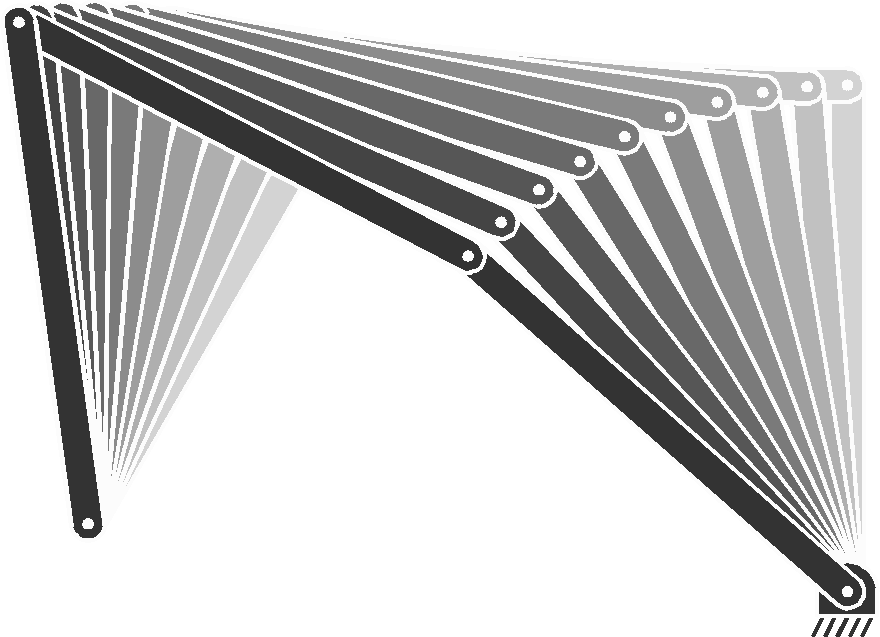
\includegraphics[width=.9\textwidth]{images/IK_nullspace01.png}
	\caption{Moving the first joint as secondary task}
	\label{fig:nullspace1}
\end{subfigure}
\hfill
\begin{subfigure}[b]{.23\textwidth}
	\centering
	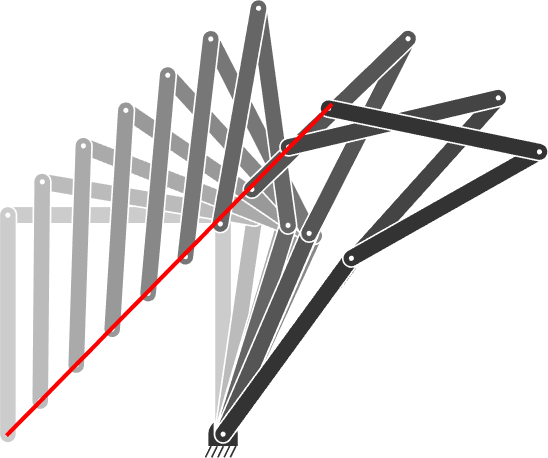
\includegraphics[width=.9\textwidth]{images/IK_nullspace02.png}
	\caption{Orientation tracking a as secondary task}
\end{subfigure}
\hfill
\begin{subfigure}[b]{.17\textwidth}
	\centering
	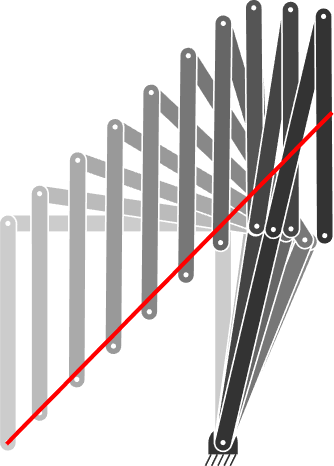
\includegraphics[width=.8\textwidth]{images/IK_nullspace03.png}
	\caption{Position tracking as secondary task}
\end{subfigure}
\hfill
\begin{subfigure}[b]{.34\textwidth}
	\centering
	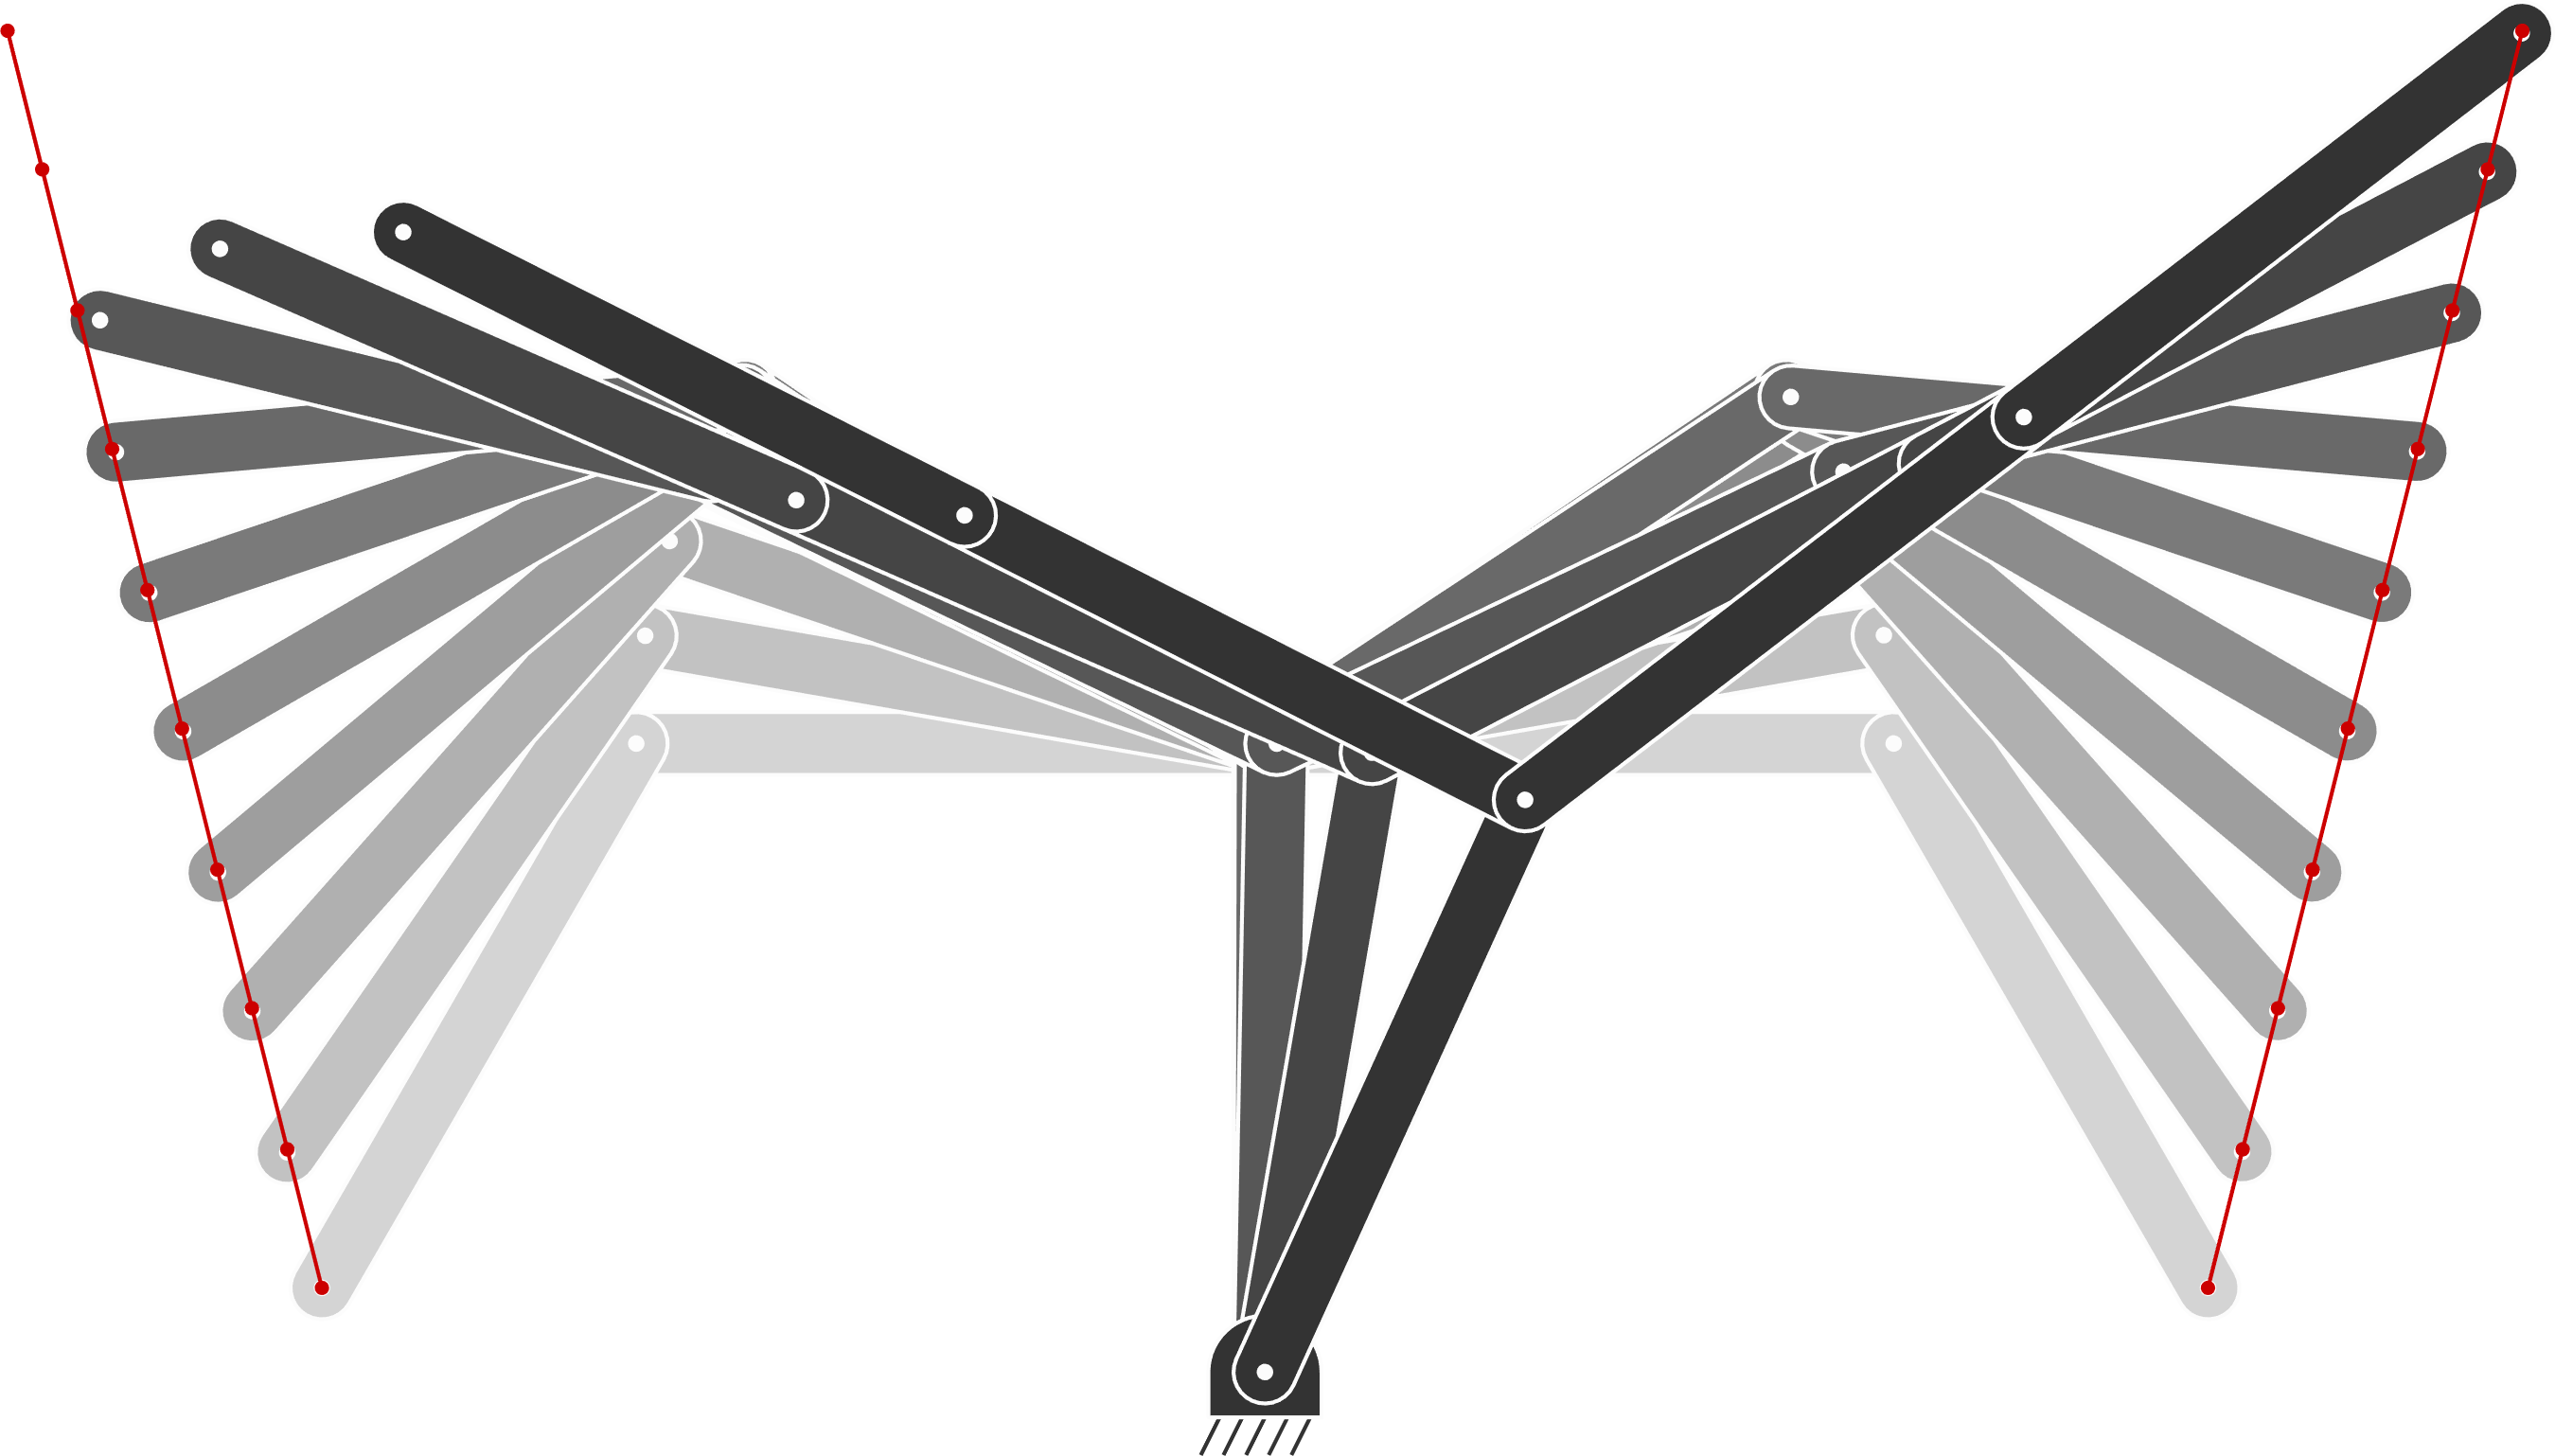
\includegraphics[width=.9\textwidth]{images/IK_nullspace04.png}
	\caption{Tracking of a moving object with the right hand as secondary task}
\end{subfigure}
\caption{\footnotesize
Examples of nullspace controllers. The red paths represent the trajectories of moving objects that need to be tracked by the robot end-effectors.
}
\label{fig:nullspace}
\end{figure}

In \eqref{eq:IK_LS}, the pseudoinverse provides a single least norm solution. This result can be generalized to obtain all solutions of the linear system with
\begin{equation}
	\bm{\dot{\bm{x}}} = \bm{J}^\psin\!(\bm{x}) \; \bm{\dot{f}} + \bm{N}\!(\bm{x}) \; \bm{g}(\bm{x}),
	\label{eq:IK_nullspace}
\end{equation}
where $\bm{g}(\bm{x})$ is any desired gradient function and $\bm{N}\!(\bm{x})$ the \textbf{nullspace projection operator}
\begin{equation*}
	\bm{N}\!(\bm{x}) = \bm{I} - \bm{J}(\bm{x})^\psin \bm{J}(\bm{x}). 
\end{equation*}

In the above, the solution is unique if and only if $\bm{J}(\bm{x})$ has full column rank, in which case $\bm{N}(\bm{x})$ is a zero matrix. 

An alternative way of computing the nullspace projection matrix, numerically more robust, is to exploit the singular value decomposition
\begin{equation*}
  \bm{J}^\psin\!=\!\bm{U}\bm{\Sigma}\bm{V}^\trsp,
\end{equation*}
to compute
\begin{equation*}
  \bm{N} = \bm{\tilde{U}} \bm{\tilde{U}}^\trsp,
  %sp = (sum(S,2)<1E-1); %Span of zero rows
  %N = U(:,sp) * U(:,sp)';
  %N = U * [0 0 0; 0 0 0; 0 0 1] * U'
\end{equation*}
where $\bm{\tilde{U}}$ is a matrix formed by the columns of $\bm{U}$ that span for the corresponding zero rows in $\bm{\Sigma}$.

Figure \ref{fig:nullspace} presents examples of nullspace controllers. Figure \ref{fig:nullspace1} shows a robot controller keeping its end-effector still as primary objective, while trying to move the first joint as secondary objective, which is achieved with the controller 
\begin{equation*}
	\bm{\dot{\bm{x}}} = \bm{J}^\psin\!(\bm{x}) \!\begin{bmatrix}0\\0\end{bmatrix} + \bm{N}\!(\bm{x}) \!\begin{bmatrix}1\\0\\0\end{bmatrix}.
\end{equation*}

%Tracking target with right hand if possible
%Tracking target with left hand
%\begin{align*}
%	\bm{\dot{\bm{x}}}
%	&= {\bm{J}^\ty{L}}^{\,\psin} \; \bm{\dot{f}}^\ty{L}
%	+ \bm{N}^\ty{L} \; {\bm{J}^\ty{R}}^{\,\psin} \; \bm{\dot{f}}^\ty{R}
%	\\
%	&= {\bm{J}^\ty{L}}^{\,\psin} \; (\bm{\hat{f}}^\ty{L}_t-\bm{f}^\ty{L})
%	+ \bm{N}^\ty{L} \; {\bm{J}^\ty{R}}^{\,\psin} \; (\bm{\hat{f}}^\ty{R}-\bm{f}^\ty{R})
%\end{align*}
%# Prioritized control (left tracking as prioritized task)
%dfl = (param.Mu[:2] - f[:2,0]) * 10 # Left hand correction
%dfr = (param.Mu[2:] - f[2:,0]) * 10 # Right hand correction
%Jl = J[:2,:] # Jacobian for left hand 
%Jr = J[2:,:] # Jacobian for right hand
%pinvJl = np.linalg.inv(Jl.T @ Jl + np.eye(param.nbVarX) * 1e1) @ Jl.T # Damped pseudoinverse
%Nl = np.eye(param.nbVarX) - pinvJl @ Jl # Nullspace projection operator
%ul = pinvJl @ dfl # Command for position tracking
%JrNl = Jr @ Nl
%pinvJrNl = JrNl.T @ np.linalg.inv(JrNl @ JrNl.T + np.eye(2) * 1e4) # Damped pseudoinverse
%ur = pinvJrNl @ (dfr - Jr @ ul) # Command for right hand tracking (with left hand tracking prioritized)
%u = ul + Nl @ ur # Control commands


%Indeed, we can see that for any vector/matrix $\bm{V}$, the nullspace projection ensures that it does not affect the minimization
%\begin{align}
%  \bm{E} &= \bm{Y} - \bm{X} \bm{\hat{A}} \\
%  &= \bm{Y} - \bm{X} \Big(\bm{X}^\trsp {(\bm{X}\bm{X}^\trsp)}^{-1} \bm{Y} + \overbrace{\big(\bm{I} - \bm{X}^\trsp {(\bm{X}\bm{X}^\trsp)}^{-1}  \bm{X}\big)}^{\bm{N}} \bm{V} \Big) \\
%  &= \bm{Y} - \bm{X}\bm{X}^\trsp {(\bm{X}\bm{X}^\trsp)}^{-1} \bm{Y} + \bm{X}\big(\bm{I} - \bm{X}^\trsp {(\bm{X}\bm{X}^\trsp)}^{-1}  \bm{X}\big) \bm{V} \\
%  &= \bm{Y} - \bm{Y} + \big(\bm{X} - \bm{X}\bm{X}^\trsp {(\bm{X}\bm{X}^\trsp)}^{-1}\bm{X}\big) \bm{V} \\
%  &= \big(\bm{X} - \bm{X}\big) \bm{V} \\
%  &= \bm{0} \;\bm{V}
%\end{align}

%This can for example be implemented in Matlab/Octave with
%\begin{verbatim}
%            [U,S,V] = svd(pinv(X))
%            sp = sum(S,2) < 1E-1
%            N = U(:,sp) * U(:,sp)'
%\end{verbatim}



%%%%%%%%%%%%%%%%%%%%%%%%%%%%%%%%%%%%%%%%%%%%%%%%%%%%%%%%%%%%%%%%%%%%%%%%%%%%%%%%%
\section{Encoding with basis functions}\label{sec:basisfcts}
\begin{flushright}
\filename{MP.*}
\end{flushright}

Basis functions can be used to encode signals in a compact manner through a weighted superposition of basis functions, acting as a dictionary of simpler signals that are superposed to form more complex signals. %It can be used to provide prior information about the encoded signals (inductive bias).

Basis functions can for example be used to encode trajectories, whose input is a 1D time variable and whose output can be multidimensional. For basis functions $\bm{\phi}(t)$ described by a time or phase variable $t$, the corresponding continuous signal $\bm{x}(t)$ is encoded with $\bm{x}(t) = \bm{\phi}(t) \, \bm{w}$, with $t$ a continuous time variable and $\bm{w}$ a vector containing the superposition weights. Basis functions can also be employed in a discretized form by providing a specific list of time steps, which is the form we will employ next. 

The term \emph{movement primitive} is often used in robotics to refer to the use of basis functions to encode trajectories. It corresponds to an organization of continuous motion signals in the form of a superposition in parallel and in series of simpler signals, which can be viewed as ``building blocks'' to create more complex movements, see Fig.~\ref{fig:MP}. This principle, coined in the context of motor control \cite{MussaIvaldi94}, remains valid for a wide range of continuous time signals (for both analysis and synthesis).

The simpler form of \emph{movement primitives} consists of encoding a movement as a weighted superposition of simpler movements. The compression aims at working in a subspace of reduced dimensionality, while denoising the signal and capturing the essential aspects of a movement. 
%This can be illustrated as basic building blocks that can be differently assembled to form more elaborated movements, often referred to as \emph{movement primitives} (MP).

%%%%%%%%%%%%%%%%%%%%%%%%%%%%%%%%%%%%%%%%%%%%%%%%%%%%%%%%%%%%%%%%%%%%%%%%%%%%%%%%%
\subsection{Univariate trajectories}

A univariate trajectory $\bm{x}^\tp{1D}\in\mathbb{R}^T$ of $T$ datapoints can be represented as a weighted sum of $K$ basis functions with
\begin{equation}
	\bm{x}^\tp{1D} = \sum_{k=1}^{K} \bm{\phi}_{k} \; w^\tp{1D}_k = \bm{\phi} \; \bm{w}^\tp{1D},
\end{equation}
where $\bm{\phi}$ can be any set of basis functions, including some common forms that are presented below (see also \cite{Calinon19MM} for more details).


%%%%%%%%%%%%%%%%%%%%%%%%%%%%%%%%%%%%%%%%%%%%%%%%%%%%%%%%%%%%%%%%%%%%%%%%%%%%%%%%%
\subsubsection*{Piecewise constant basis functions}

\begin{figure}
\centering
\begin{subfigure}[c]{.45\textwidth}
	\centering
	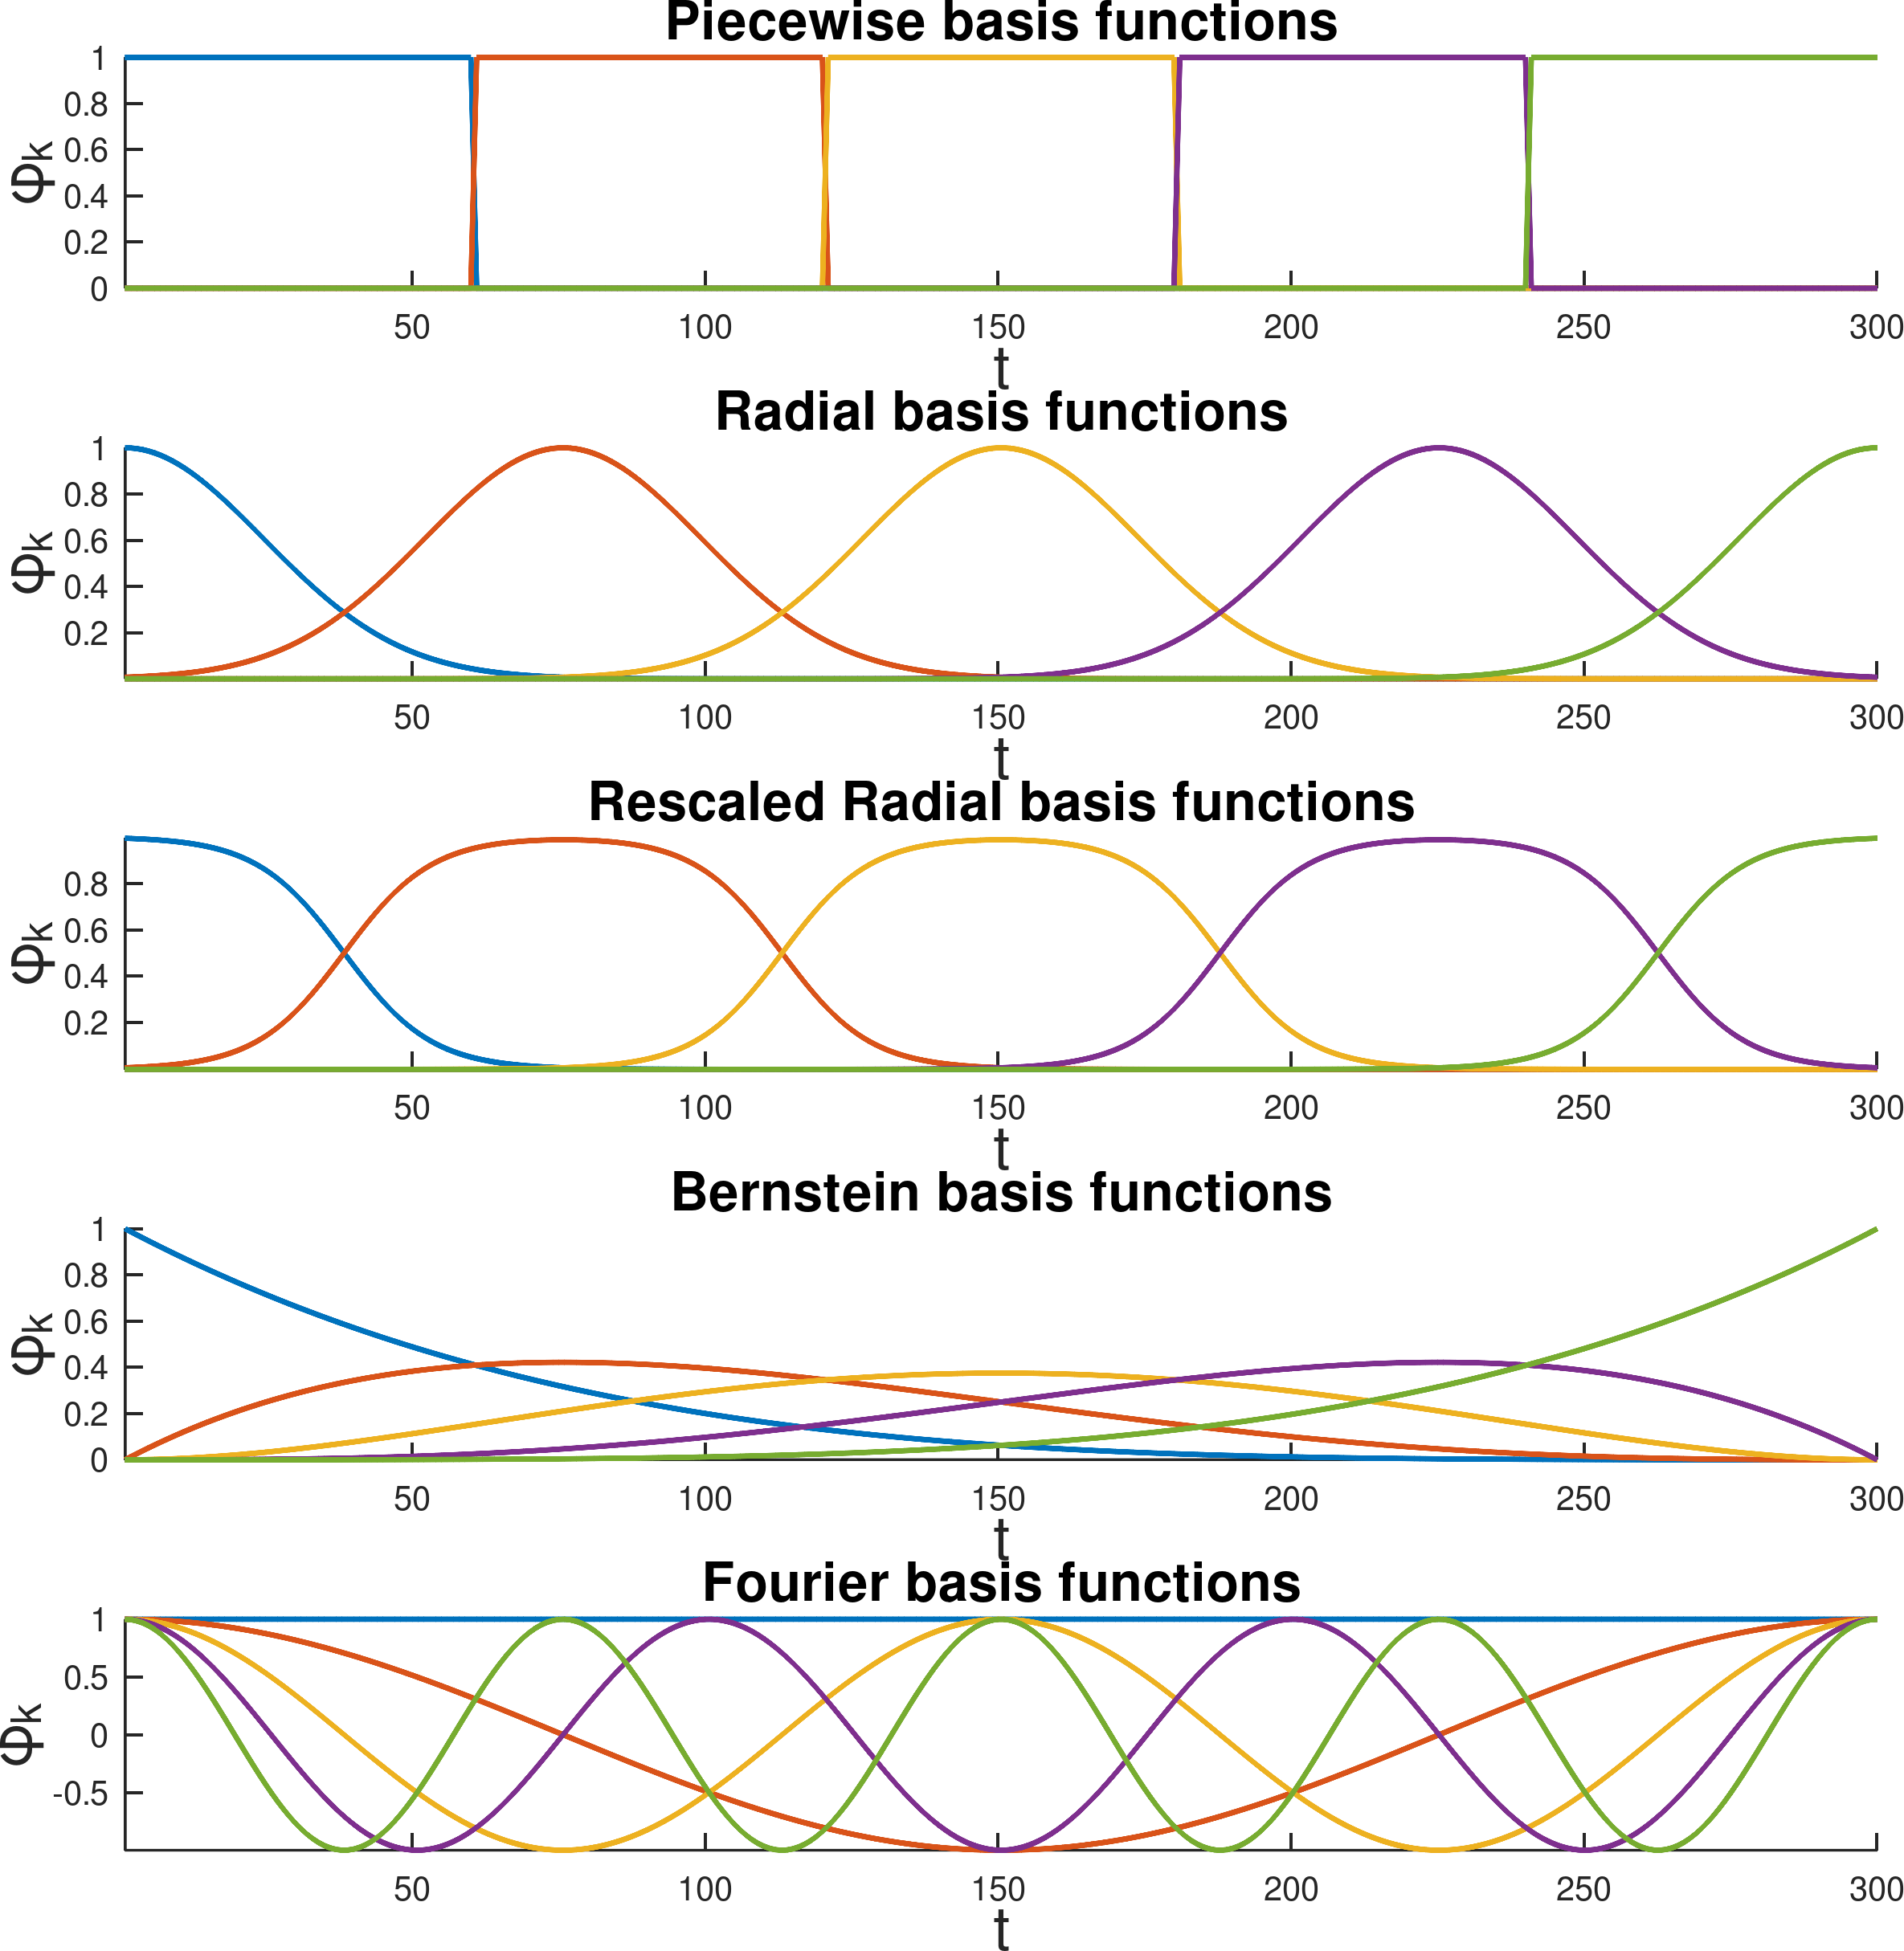
\includegraphics[width=\textwidth]{images/MP_basisFcts01.png}
\end{subfigure}
\hfill
\begin{subfigure}[c]{.45\textwidth}
	\centering
	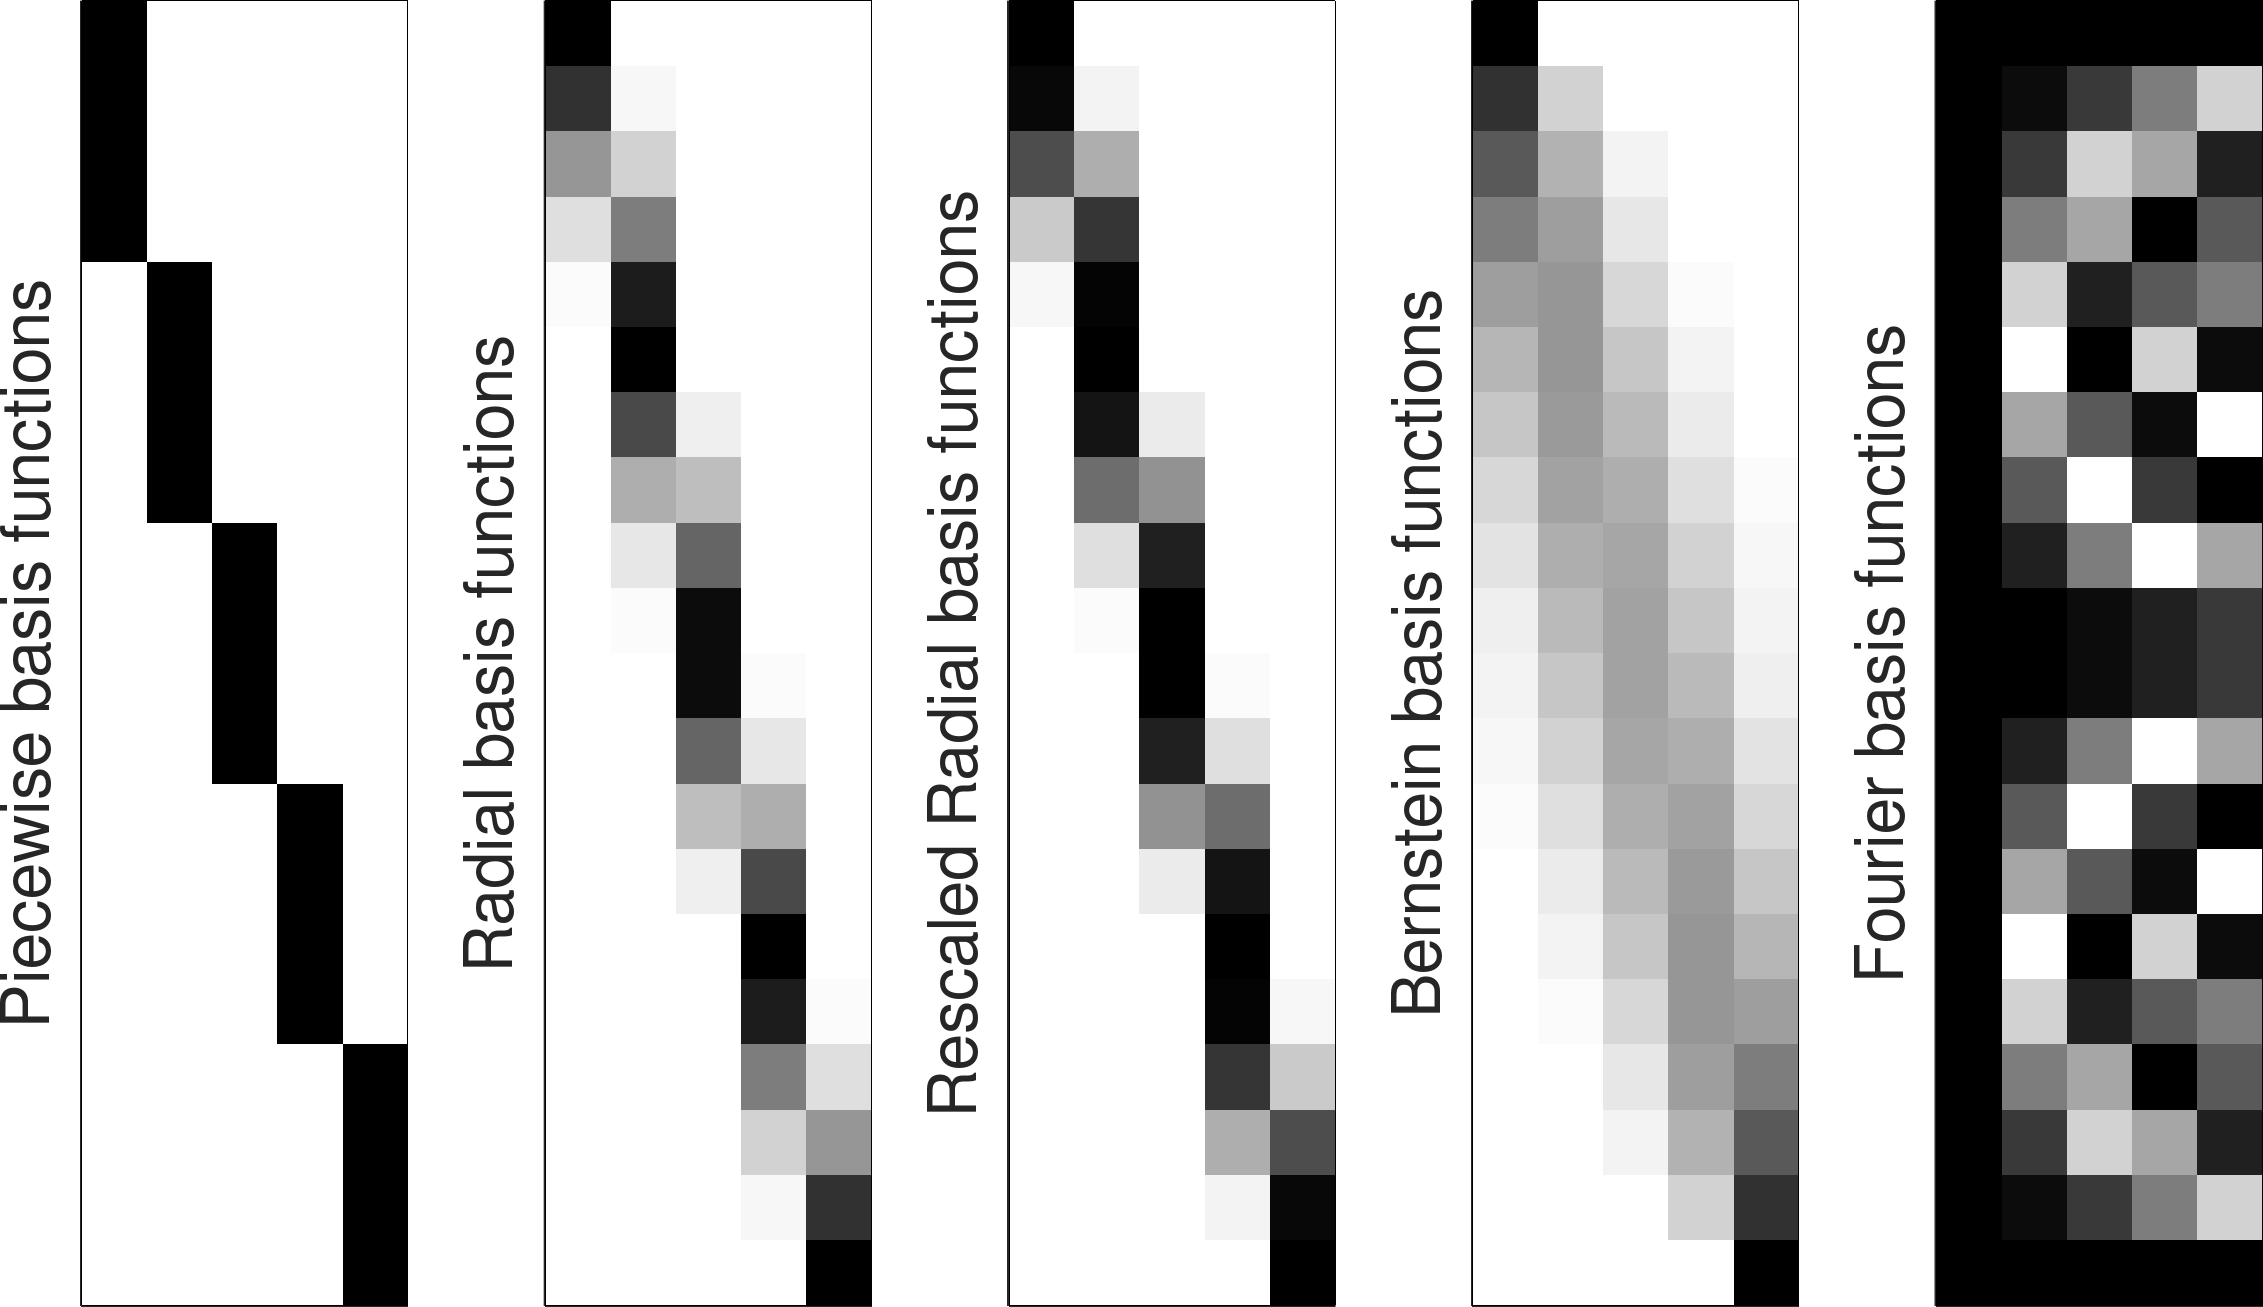
\includegraphics[width=\textwidth]{images/MP_basisFcts_mat01.png}
\end{subfigure}
\caption{\footnotesize
Examples of basis functions. \emph{Left:} Representation in timeline form for $K=5$ and $T=300$. \emph{Right:} Representation in matrix form for $K=5$ and $T=20$, with a grayscale colormap where white pixels are $0$ and black pixels are $1$.
}
\label{fig:MP}
\end{figure}

Piecewise constant basis functions can be computed in matrix form as
\begin{equation}
	\bm{\phi} = \bm{I}_K \otimes \bm{1}_{\frac{T}{K}},
\end{equation}
where $\bm{I}_K$ is an identity matrix of size $K$ and $\bm{1}_{\frac{T}{K}}$ is a vector of length $\frac{T}{K}$ compose of unit elements, see Fig.~\ref{fig:MP}.


%%%%%%%%%%%%%%%%%%%%%%%%%%%%%%%%%%%%%%%%%%%%%%%%%%%%%%%%%%%%%%%%%%%%%%%%%%%%%%%%%
\subsubsection*{Radial basis functions (RBFs)}

Gaussian radial basis functions (RBFs) can be computed in matrix form as
\begin{equation}
	\bm{\phi} = \exp(-\lambda \; \bm{E} \odot \bm{E}),
	\quad\text{with}\quad \bm{E} = \bm{t} \; \bm{1}_K^\trsp - \bm{1}_T \; {\bm{\mu}^\tp{s}}^\trsp,
\end{equation}
where $\lambda$ is bandwidth parameter, $\odot$ is the elementwise (Hadamard) product operator, $\bm{t}\in\mathbb{R}^T$ is a vector with entries linearly spaced between $0$ to $1$, $\bm{\mu}^\tp{s}\in\mathbb{R}^K$ is a vector containing the RBF centers linearly spaced on the $[0,1]$ range, and the $\exp(\cdot)$ function is applied to each element of the matrix, see Fig.~\ref{fig:MP}. 

RBFs can also be employed in a rescaled form by replacing each row $\bm{\phi}_k$ with $\frac{\bm{\phi}_k}{\sum_{i=1}^K\bm{\phi}_i}$.

%sigma = 1 / (nbFct-2); %Standard deviation
%tMu = linspace(t(1)-1/(nbFct-3), t(end)+1/(nbFct-3), nbFct); %With offset to avoid border effects

%Optional rescaling
%phi = phi ./ repmat(sum(phi,2), 1, nbFct); 


%%%%%%%%%%%%%%%%%%%%%%%%%%%%%%%%%%%%%%%%%%%%%%%%%%%%%%%%%%%%%%%%%%%%%%%%%%%%%%%%%
\subsubsection*{Bernstein basis functions}

Bernstein basis functions (used for B\'ezier curves) can be computed as
\begin{equation}
	\bm{\phi}_k = \frac{(K-1)!}{(k-1)!(K-k)!} \; {(\bm{1}_T-\bm{t})}^{K-k} \;\odot\; \bm{t}^{k-1},
\end{equation}
$\forall k\in\{1,\ldots,K\}$, where $\bm{t}\in\mathbb{R}^T$ is a vector with entries linearly spaced between $0$ to $1$, and $(\cdot)^d$ is applied elementwise, see Fig.~\ref{fig:MP}.


%%%%%%%%%%%%%%%%%%%%%%%%%%%%%%%%%%%%%%%%%%%%%%%%%%%%%%%%%%%%%%%%%%%%%%%%%%%%%%%%%
\subsubsection*{Fourier basis functions}

Fourier basis functions can be computed in matrix form as
\begin{equation}
	\bm{\phi} = \exp(\bm{t} \, \bm{\tilde{k}}^\trsp \, 2\pi i), 
\end{equation}
where the $\exp(\cdot)$ function is applied to each element of the matrix, $\bm{t}\in\mathbb{R}^T$ is a vector with entries linearly spaced between $0$ to $1$, $\bm{\tilde{k}}={[-K\!+\!1,-K\!+\!2,\ldots,K\!-\!2,K\!-\!1]}^\trsp$, and $i$ is the imaginary unit ($i^2=-1$).

If $\bm{x}$ is a real and even signal, the above formulation can be simplified to
\begin{equation}
	\bm{\phi} = \cos(\bm{t} \, \bm{k}^\trsp \, 2\pi i),
	\label{eq:dct} 
\end{equation}
with $\bm{k}={[0,1,\ldots,K\!-\!2,K\!-\!1]}^\trsp$, see Fig.~\ref{fig:MP}.

%	%Computation for general signals (incl. complex numbers)
%	d = ceil((K-1)/2);
%	k = -d:d;
%	phi = exp(t' * k * 2 * pi * 1i); 
%	%phi = cos(t' * k * 2 * pi); %Alternative computation for real signal
		
%	%Alternative computation for real and even signal
%	k = 0:K-1;
%	phi = cos(t' * k * 2 * pi);
%	%phi(:,2:end) = phi(:,2:end) * 2;
%	%invPhi = cos(k' * t * 2 * pi) / nbData;
%	%invPsi = kron(invPhi, eye(param.nbVar));

%With such definition, we can see that for a given time step $t$, the signal is constructed with the Fourier series
%\begin{equation}
%	x_t = \sum_{k=-K+1}^{K-1} w_k \exp(t \, k \, 2\pi i).
%\end{equation}

Indeed, we first note that $\exp(ai)$ is composed of a real part and an imaginary part with $\exp(ai)=\cos(a)+i\sin(a)$. We can see that for a given time step $t$, a real state $x_t$ can be constructed with the Fourier series 
\begin{align*}
	x_t &= \sum_{k=-K+1}^{K-1} w_k \exp(t \, k \, 2\pi i)\\
	&=\sum_{k=-K+1}^{K-1} w_k \cos(t \, k \, 2\pi)\\
	&= w_0 + \sum_{k=1}^{K-1} 2 w_k \cos(t \, k \, 2\pi),
\end{align*}
where we used the properties $\cos(0)=1$ and $\cos(-a)=\cos(a)$ of the cosine function. Since we do not need direct correspondences between the Fourier transform and discrete cosine transform as in the above, we can omit the scaling factors for $w_k$ and directly write the decomposition as in \eqref{eq:dct}. 


%%%%%%%%%%%%%%%%%%%%%%%%%%%%%%%%%%%%%%%%%%%%%%%%%%%%%%%%%%%%%%%%%%%%%%%%%%%%%%%%%
\subsection{Multidimensional outputs}

A multivariate trajectory $\bm{x}\in\mathbb{R}^{DT}$ of $T$ datapoints of dimension $D$ can similarly be computed as
\begin{equation}
	\bm{x} = \sum_{k=1}^{K} \bm{\Psi}_{k} \; w_k = \bm{\Psi} \; \bm{w},
	\quad\text{with}\quad \bm{\Psi} = \bm{\phi} \otimes \bm{I} = \left[\begin{matrix}
	\bm{I}\phi_{1,1} & \bm{I}\phi_{2,1} & \cdots & \bm{I}\phi_{K,1} \\
	\bm{I}\phi_{1,2} & \bm{I}\phi_{2,2} & \cdots & \bm{I}\phi_{K,2} \\
	\vdots & \vdots & \ddots & \vdots \\
	\bm{I}\phi_{1,T} & \bm{I}\phi_{2,T} & \cdots & \bm{I}\phi_{K,T}  
	\end{matrix}\right], \label{eq:Psi}
\end{equation}
where $\otimes$ the Kronecker product operator and $\bm{I}$ is an identity matrix of size $D\times D$. 

In the above, $\bm{I}$ can alternatively be replaced by a rectangular matrix $\bm{S}$ acting as a coordination matrix. 


%%%%%%%%%%%%%%%%%%%%%%%%%%%%%%%%%%%%%%%%%%%%%%%%%%%%%%%%%%%%%%%%%%%%%%%%%%%%%%%%%
\subsection{Multidimensional inputs}
\begin{flushright}
\filename{spline2d.*}
\end{flushright}

\begin{wrapfigure}{r}{.68\textwidth}
\centering
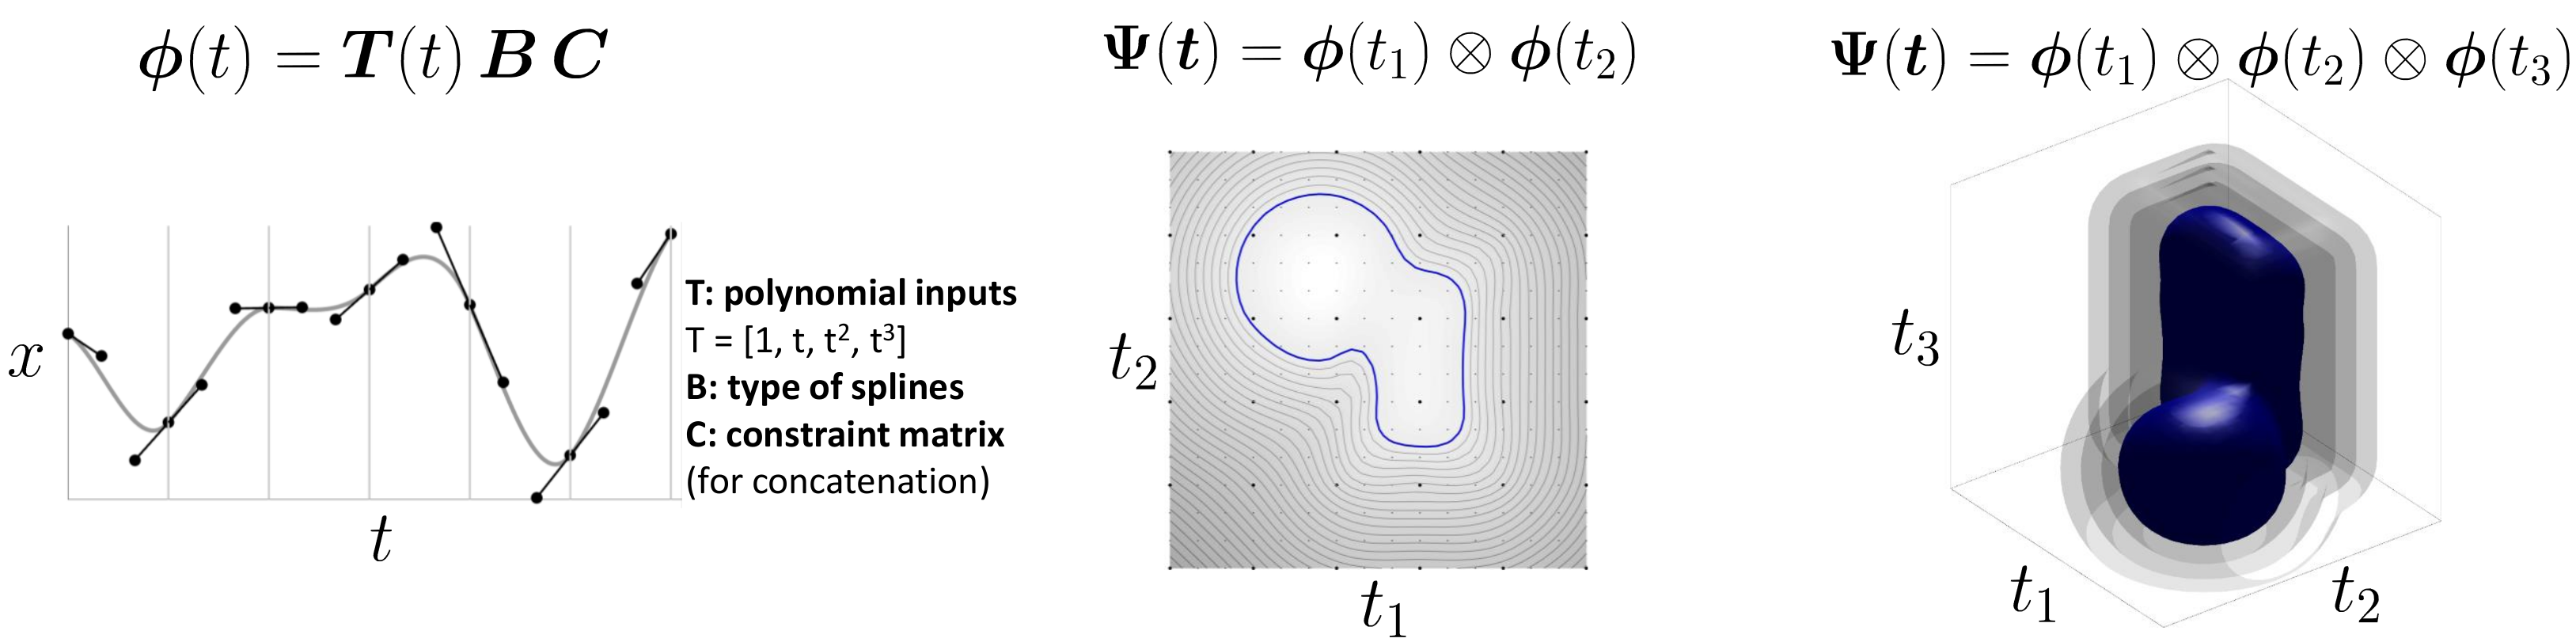
\includegraphics[width=.66\textwidth]{images/Bezier_1D2D3D01.png}
\caption{\footnotesize
Concatenated Bernstein basis functions used with inputs of various dimensions to encode signed distance functions (SDFs). 
\emph{Left:} Concatenation of $6$ cubic Bézier curves with a 1D input (time variable $t$). 
\emph{Center:} Concatenation of $5\!\times\!5$ cubic Bézier curves with a 2D input. 
\emph{Right:} Concatenation of $5\!\times\!5\!\times\!5$ cubic Bézier curves with a 3D input.
Each cubic Bézier curve corresponds to the superposition of 4 Bernstein basis functions, with superposition weights acting as control points (displayed as black points in the 1D example), with constraints on the control points ensuring continuity.
}
\label{fig:Bezier_1D2D3D01}
\end{wrapfigure}

Basis functions can also be used to encode signals generated by multivariate inputs $t_i$. For example, a Bézier surface uses two input variables $t_1$ and $t_2$ to cover a spatial range and generates an output variable describing the height of the surface within this rectangular region. This surface (represented as a colormap in Fig.~\ref{fig:Bezier_1D2D3D01}-\emph{center}) can be constructed from a 1D input signal by leveraging the Kronecker product operation, namely
\begin{equation}
	\bm{\Psi} = \bm{\phi} \,\otimes\, \bm{\phi}
\end{equation}
in matrix form, or
\begin{equation}
	\bm{\Psi}(\bm{t}) = \bm{\phi}(t_1) \,\otimes\, \bm{\phi}(t_2)
	\label{eq:Psi2D_analytic}
\end{equation}
in analytic form.

When using splines of the form $\bm{\phi}(t)=\bm{T}(t)\bm{B}\bm{C}$, \eqref{eq:Psi2D_analytic} can equivalently be computed as
\begin{equation}
	\bm{\Psi}(\bm{t}) = \big(\bm{T}(t_1) \,\otimes\, \bm{T}(t_2)\big) \, \big(\bm{B}\bm{C} \,\otimes\, \bm{B}\bm{C}\big),
\end{equation}
which means that $\big(\bm{B}\bm{C} \,\otimes\, \bm{B}\bm{C}\big)$ can be precomputed.

As for the unidimensional version, we still maintain a linear reconstruction $\bm{x} = \bm{\Psi} \, \bm{w}$, where $\bm{x}$ and $\bm{w}$ are vectorized versions of surface heights and superposition weights, which can be reorganized as 2D arrays if required.

Successive Kronecker products can be used so that any number of input and output dimensions ${d^\tp{in}}$ and ${d^\tp{out}}$ can be considered, with 
\begin{equation}
	\bm{\Psi} = \underbrace{\bm{\phi} \,\otimes\, \bm{\phi} \,\otimes \cdots \otimes\,  \bm{\phi}}_{d^\tp{in}} \,\otimes\,  \bm{I}_{d^\tp{out}}.
\end{equation}

For example, a vector field in 3D can be encoded with basis functions
\begin{equation}
	\bm{\Psi} = \bm{\phi} \,\otimes\, \bm{\phi} \,\otimes\, \bm{\phi} \,\otimes\, \bm{I}_3,
\end{equation}
where $\bm{I}_3$ is a $3\!\times\!3$ identity matrix to encode the 3 elements of the vector. 

Figure \ref{fig:Bezier_1D2D3D01} shows examples with various input dimensions to encode a signed distance field (SDF). In Fig.~\ref{fig:Bezier_1D2D3D01}-\emph{center}, several equidistant contours are displayed as closed paths, with the one corresponding to the object contour (distance zero) represented in blue. In Fig.~\ref{fig:Bezier_1D2D3D01}-\emph{right}, several isosurfaces are displayed as 3D shapes, with the one corresponding to the object surface (distance zero) represented in blue. A marching algorithm has been used here for visualization purpose to compute closed contours (in 2D) and isosurfaces (in 3D). %, but can also be exploited if an explicit definition of shapes is required (instead of an implicit surface representation).

The analytic expression provided by the proposed encoding can be used to express the derivatives as analytic expressions, which is useful for control and planning problem, such as moving closer or away from objects, or orienting the robot gripper to be locally aligned with the surface of an object.


%%%%%%%%%%%%%%%%%%%%%%%%%%%%%%%%%%%%%%%%%%%%%%%%%%%%%%%%%%%%%%%%%%%%%%%%%%%%%%%%%
\subsection{Derivatives}

By using basis functions as analytic expressions, the derivatives are easy to compute. For example, for 2D inputs as in \eqref{eq:Psi2D_analytic}, we have   
\begin{equation}
	\frac{\partial\bm{\Psi}(\bm{t})}{\partial t_1} = \frac{\partial\bm{\phi}(t_1)}{\partial t_1} \,\otimes\, \bm{\phi}(t_2),
	\qquad\qquad
	\frac{\partial\bm{\Psi}(\bm{t})}{\partial t_2} = \bm{\phi}(t_1) \,\otimes\, \frac{\partial\bm{\phi}(t_2)}{\partial t_2},
	\label{eq:parialPsi}
\end{equation}
providing the derivatives of $\bm{\Psi}(\bm{t})$ with respect to $\bm{t}$ expressed as
\begin{equation}
	\bm{\nabla}\bm{\Psi}(\bm{t}) = \frac{\partial\bm{\Psi}(\bm{t})}{\partial t_1} \,\otimes\, \frac{\partial\bm{\Psi}(\bm{t})}{\partial t_2},
	\label{eq:dPsi}
\end{equation}
which can be used to compute the 2D gradient of the SDF at location $\bm{t}$ with
\begin{equation}
	\bm{\nabla}x = \bm{\nabla}\bm{\Psi}(\bm{t}) \, \bm{w}.
\end{equation}

When using splines of the form $\bm{\phi}(t)=\bm{T}(t)\bm{B}\bm{C}$, the derivatives in \eqref{eq:parialPsi} are simply computed as $\frac{\partial\bm{\phi}(t)}{\partial t}=\frac{\partial\bm{T}(t)}{\partial t} \bm{B}\bm{C}$. For a cubic splines, it corresponds to $\bm{T}(t) = [1,t,t^2,t^3]$ and $\frac{\partial\bm{T}(t)}{\partial t} = [0,1,2t,3t^2]$.\newline


%%%%%%%%%%%%%%%%%%
\noindent\textbf{Example: finding the closest point on a contour}\newline

By modeling a signed distance function as $x = f(\bm{t})$, the derivatives can for example be used to find a point on the contour (with distance zero). Such problem can be solved with Gauss--Newton optimization with the cost $c(\bm{t})= \frac{1}{2} f(\bm{t})^2$, by starting from an initial guess $\bm{t}_0$. In the above example, the Jacobian is then given by
\begin{equation}
	\bm{J}(\bm{t}) = \begin{bmatrix} \frac{\partial\bm{\Psi}(\bm{t})}{\partial t_1} \,\bm{w} 
	\\[2mm] \frac{\partial\bm{\Psi}(\bm{t})}{\partial t_2} \,\bm{w} \\ \vdots \end{bmatrix},
	\label{eq:J_SDF}
\end{equation}
and the update can be computed recursively with
\begin{equation}
	\bm{t}_{k+1} \;\leftarrow\; \bm{t}_k - \alpha \bm{J}(\bm{t}_k)^\psin f(\bm{t}_k),
	\label{eq:update_SDF}
\end{equation}
as in Equation \eqref{eq:GaussNewtonUpdate}, where $\bm{J}(\bm{t}_k)^\trsp f(\bm{t}_k)$ is a gradient and $\bm{J}(\bm{t}_k)^\trsp \bm{J}(\bm{t}_k)$ a Hessian matrix, and $\alpha$ is a line search parameter.\newline


%%%%%%%%%%%%%%%%%%
\noindent\textbf{Example: finding two contour points with closest distance}\newline

For two shapes encoded as SDFs $f_1(\bm{t}_1)$ and $f_2(\bm{t}_2)$ using basis functions, finding the shortest segment between the two shapes boils down to the Gauss--Newton optimization of a pair of points $\bm{t}_1$ and $\bm{t}_2$ are expressed in their respective shape coordinate frame and are organized as $\bm{t} = \begin{bmatrix} \bm{t}_1 \\ \bm{t}_2 \end{bmatrix}$, with the cost
\begin{equation}
	c(\bm{t}) = \frac{1}{2} \, f_1(\bm{t}_1)^2 + \frac{1}{2} \, f_2(\bm{t}_2)^2 + \frac{1}{2} \, \|\bm{A} \, \bm{t}_2 + \bm{b} - \bm{t}_1\|^2,
\end{equation}
which is composed of quadratic residual terms, where $\bm{A}$ and $\bm{b}$ are the rotation matrix and translation vector offset between the two objects, respectively. The Jacobian of the residual terms in the above cost is given by
\begin{equation}
	\bm{J}(\bm{t}) = \begin{bmatrix} \bm{J}_1(\bm{t}_1) & \bm{0} \\ \bm{0} & \bm{J}_2(\bm{t}_2) \\ -\bm{I} & \bm{A} \end{bmatrix},
\end{equation}
where $\bm{J}_1(\bm{t}_1)$ and $\bm{J}_2(\bm{t}_2)$ are the derivatives of the two SDFs as given by \eqref{eq:J_SDF}.

Similarly to \eqref{eq:update_SDF}, the Gauss--Newton update step is then given by
\begin{equation}
	\bm{t}_{k+1} \;\leftarrow\; \bm{t}_k - \alpha \bm{J}(\bm{t}_k)^\psin 
	\begin{bmatrix} f_1(\bm{t}_{1,k}) \\ f_2(\bm{t}_{2,k}) \\ \bm{A} \, \bm{t}_{2,k} + \bm{b} - \bm{t}_{1,k} \end{bmatrix}.
\end{equation}

A prioritized optimization scheme can also be used to have the two points on the shape boundaries as primary objective and to move these points closer as secondary objective, with a corresponding Gauss--Newton update step given by
\begin{align}
	\bm{t}_{k+1} &\leftarrow\; \bm{t}_k - \alpha_1 \bm{J}_{12}^\psin \begin{bmatrix} f_1(\bm{t}_{1,k}) \\ f_2(\bm{t}_{2,k}) \end{bmatrix} 	
	+ \alpha_2 \bm{N}_{12} \; \bm{J}_{3}^\psin \; (\bm{A} \, \bm{t}_{2,k} + \bm{b} - \bm{t}_{1,k}), \\	
	\text{where}\quad
	\bm{J}_{12} &= \begin{bmatrix} \bm{J}_1(\bm{t}_1) & \bm{0} \\ \bm{0} & \bm{J}_2(\bm{t}_2) \end{bmatrix}, \quad
	\bm{N}_{12} = \bm{I} - \bm{J}_{12}^\psin \bm{J}_{12}, \quad
	\bm{J}_{3} = \begin{bmatrix} -\bm{I} & \bm{A} \end{bmatrix},
\end{align}
with $\alpha_1$ and $\alpha_2$ are two line search parameters.


%%%%%%%%%%%%%%%%%%%%%%%%%%%%%%%%%%%%%%%%%%%%%%%%%%%%%%%%%%%%%%%%%%%%%%%%%%%%%%%%%
\subsection{Concatenated basis functions}

When encoding entire signals, some dictionaries such as Bernstein basis functions require to set polynomials of high order to encode long or complex signals. Instead of considering a global encoding, it can be useful to split the problem as a set of local fitting problems which can consider low order polynomials. A typical example is the encoding of complex curves as a concatenation of simple Bézier curves. When concatenating curves, constraints on the superposition weights are typically considered. These weights can be represented as control points in the case of Bézier curves and splines. We typically constrain the last point of a curve and the first point of the next curve to maintain the continuity of the curve. We also typically constrain the control points before and after this joint to be symmetric, effectively imposing smoothness.

In practice, this can be achieved efficiently by simply replacing $\bm{\phi}$ with $\bm{\phi}\bm{C}$ in the above equations, where $\bm{C}$ is a tall rectangular matrix. This further reduces the number of superposition weights required in the encoding, as the constraints also reduce the number of free variables. 

For example, for the concatenation of Bézier curves, we can define $\bm{C}$ as
\begin{equation}
	\bm{C} = \begin{bmatrix}
	1 & 0 & \cdots & 0 & 0 & \cdots \\
	0 & 1 & \cdots & 0 & 0 & \cdots \\
	\vdots & \vdots & \ddots & \vdots & \vdots & \ddots \\
	0 & 0 & \cdots & 1 & 0 & \cdots \\
	0 & 0 & \cdots & 0 & 1 & \cdots \\
	0 & 0 & \cdots & 0 & 1 & \cdots \\
	0 & 0 & \cdots & -1 & 2 & \cdots \\
	\vdots & \vdots & \ddots & \vdots & \vdots & \ddots
	\end{bmatrix},
\end{equation}
where the pattern $\begin{bmatrix} 1 & 0 \\ 0 & 1 \\ 0 & 1 \\ -1 & 2 \end{bmatrix}$ is repeated for each junction of two consecutive Bézier curves. For two concatenated cubic Bézier curves, each composed of 4 Bernstein basis functions, we can see locally that this operator yields a constraint of the form
\begin{equation}
	\begin{bmatrix} w_3 \\ w_4 \\ w_5 \\ w_6 \end{bmatrix} =
	\begin{bmatrix} 1 & 0 \\ 0 & 1 \\ 0 & 1 \\ -1 & 2 \end{bmatrix} 
	\begin{bmatrix} a \\ b \end{bmatrix},
\end{equation}
which ensures that $w_4=w_5$ and $w_6=-w_3+2w_5$. These constraints guarantee that the last control point and the first control point of the next segment are the same, and that the control point before and after are symmetric with respect to this junction point, see Fig.~\ref{fig:Bezier_1D2D3D01}-\emph{left}.


%%%%%%%%%%%%%%%%%%%%%%%%%%%%%%%%%%%%%%%%%%%%%%%%%%%%%%%%%%%%%%%%%%%%%%%%%%%%%%%%%
\subsection{Batch computation of basis functions coefficients}
\label{sec:batchSDF}

Based on observed data $\bm{x}$, the superposition weights $\bm{w}$ can be estimated as a simple least squares estimate 
\begin{equation}
	\bm{w} = \bm{\Psi}^\psin \bm{x},
\end{equation}
or as the regularized version (ridge regression)
\begin{equation}
	\bm{w} = {(\bm{\Psi}^\trsp\bm{\Psi} + \lambda\bm{I})}^{-1} \bm{\Psi}^\trsp \bm{x}.
	\label{eq:ridge}
\end{equation}


%%%%%%%%%%%%%%%%%%%%%%%%%%%%%%%%%%%%%%%%%%%%%%%%%%%%%%%%%%%%%%%%%%%%%%%%%%%%%%%%%
\subsection{Recursive computation of basis functions coefficients}
\label{sec:recursiveSDF}

\begin{figure}
\centering
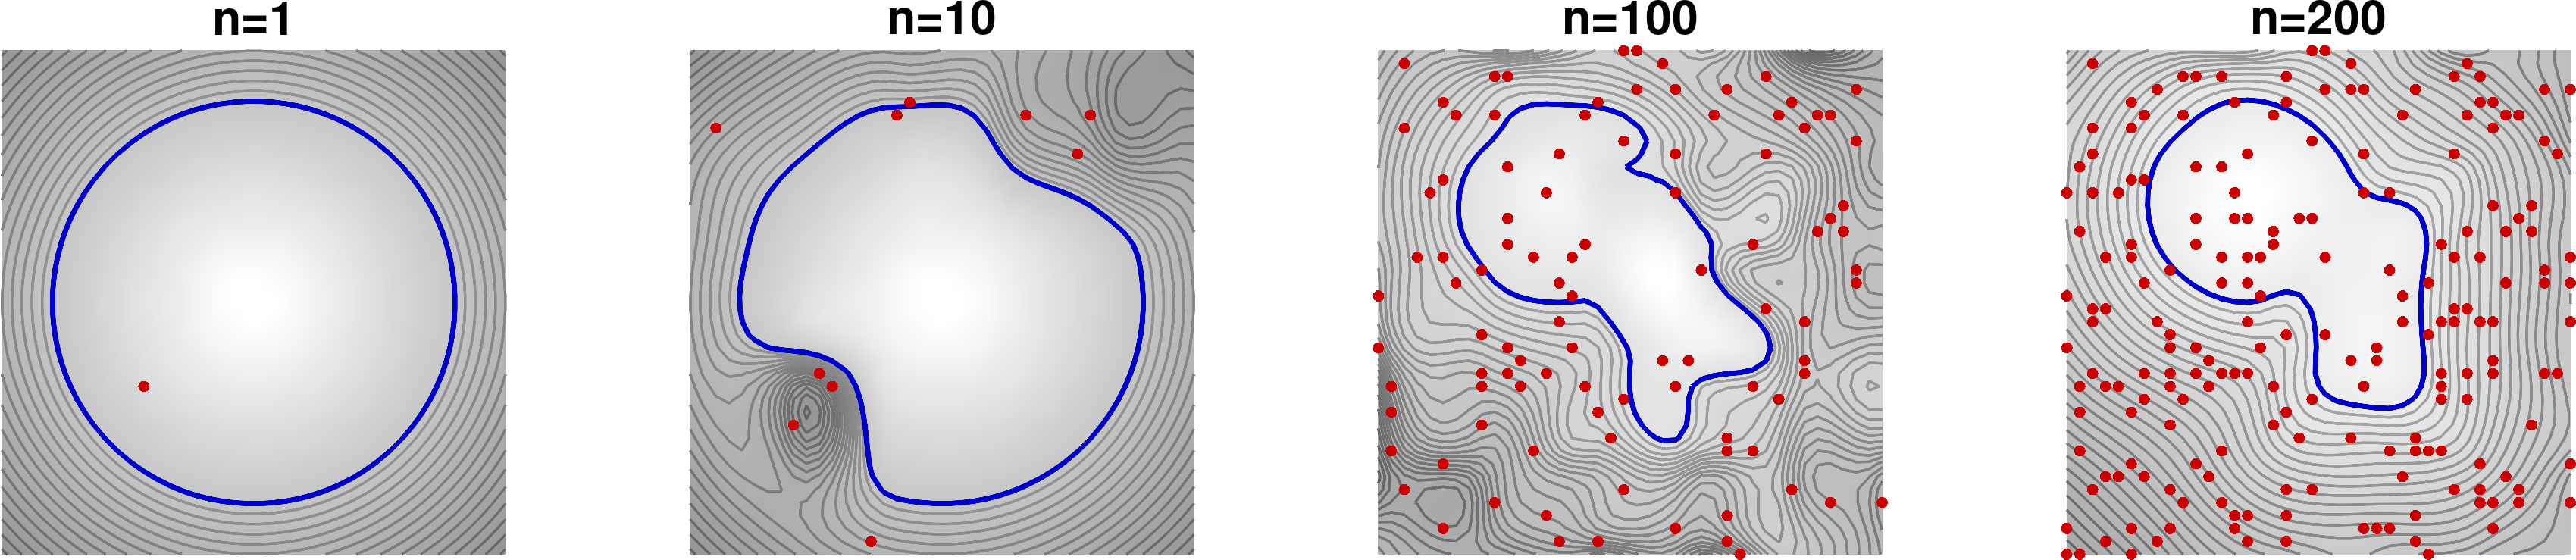
\includegraphics[width=\textwidth]{images/spline2D_RLS02.png}
\caption{\footnotesize
Iterative estimation of a 2D SDF, where the weights are initialized to form a circular object. Points are then sampled one-by-one (in red) to probe the value of the function as the sampled location. Each point used to refine the estimate and is then discarded. 
}
\label{fig:Bezier_2D_RLS}
\end{figure}

\begin{algorithm}
\caption{Recursive computation of weights}
\label{alg:splineRLS} 
$\bm{\tilde{B}} = \frac{1}{\lambda}\bm{I}$ \tcp{Initialize $\bm{\tilde{B}}$, corresponding to $(\bm{\Psi}^\trsp\bm{\Psi})^{-1}$} 
$\bm{w} = \bm{w}_0$ \tcp{Initialize superposition weights (e.g., with prior shape $\bm{w}_0$)} 
\For{$n \gets 1$ to $N$}{
	$\bm{\Psi}_n = \bm{\Psi}(\bm{t}_n)$ \tcp{Evaluate basis functions at location $\bm{t}_n$, where the corresponding datapoint is $\bm{x}_n$} 
	$\bm{K} = \bm{\tilde{B}}\bm{\Psi}_n^\trsp \left(\bm{I}+\bm{\Psi}_n\bm{\tilde{B}}\bm{\Psi}_n^\trsp\right)^{-1}$ \tcp{Compute Kalman gain $\bm{K}$} 
	$\bm{\tilde{B}} \leftarrow \bm{\tilde{B}} - \bm{K} \bm{\Psi}_n \bm{\tilde{B}}$ \tcp{Update $\bm{\tilde{B}}$} 
	$\bm{w} \leftarrow \bm{w} + \bm{K} \Big( \bm{x}_n - \bm{\Psi}_n \bm{w} \Big)$ \tcp{Update superposition weights $\bm{w}$} 
}
\end{algorithm}

The same result can be obtained by recursive computation, by providing the datapoints one-by-one or by groups of points. The algorithm starts from an initial estimate of $\bm{w}$ that is iteratively refined with the arrival of new datapoints, see Fig.~\ref{fig:Bezier_2D_RLS}.

This recursive least squares algorithm exploits the \textbf{Sherman-Morrison-Woodbury formulas} that relate the inverse of a matrix after a small-rank perturbation to the inverse of the original matrix, namely
\begin{equation}
	\left(\bm{B}+\bm{U}\bm{V}\right)^{-1} =
	\bm{B}^{-1} - \overbrace{\bm{B}^{-1}\bm{U} \left(\bm{I}+\bm{V}\bm{B}^{-1}\bm{U}\right)^{-1} \bm{V}\bm{B}^{-1}}^{\bm{E}}
	\label{eq:SMW}
\end{equation}
with $\bm{U}\!\in\!\mathbb{R}^{n\times m}$ and $\bm{V}\!\in\!\mathbb{R}^{m\times n}$. When $m\!\ll\!n$, the correction term $\bm{E}$ can be computed more efficiently than inverting $\bm{B}+\bm{U}\bm{V}$.

By defining $\bm{B}\!=\!\bm{\Psi}^\trsp\bm{\Psi}$, the above relation can be exploited to update the least squares solution \eqref{eq:ridge} when new datapoints become available. Indeed, if $\bm{\Psi}_\new = \begin{bmatrix}\bm{\Psi}, \bm{V}\end{bmatrix}$ and  $\bm{x}_\new = \begin{bmatrix}\bm{x}\\\bm{v}\end{bmatrix}$, we can see that
\begin{align}
	\bm{B}_\new
	&= \bm{\Psi}_\new^\trsp \bm{\Psi}_\new \\
	&= \bm{\Psi}^\trsp \bm{\Psi} + \bm{V}^\trsp \bm{V} \\
	&= \bm{B} + \bm{V}^\trsp \bm{V},
\end{align}
whose inverse can be computed using \eqref{eq:SMW}, yielding
\begin{equation}
	\bm{B}_\new^{-1} =
	\bm{B}^{-1} - \underbrace{\bm{B}^{-1}\bm{V}^\trsp \left(\bm{I}+\bm{V}\bm{B}^{-1}\bm{V}^\trsp\right)^{-1}}_{\bm{K}} \bm{V}\bm{B}^{-1}.
\end{equation}
This is exploited to estimate the update as
\begin{equation}
	\bm{w}_\new = \bm{w} + \bm{K} \Big( \bm{v} - \bm{V} \bm{w} \Big),
\end{equation}
with Kalman gain 
\begin{equation}
	\bm{K} = \bm{B}^{-1}\bm{V}^\trsp \left(\bm{I}+\bm{V}\bm{B}^{-1}\bm{V}^\trsp\right)^{-1}.
\end{equation}

The above equations can be used recursively, with $\bm{B}_\new^{-1}$ and $\bm{w}_\new$ the updates that will become $\bm{B}^{-1}$ and $\bm{w}$ for the next iteration. Note that the above iterative computation only uses $\bm{B}^{-1}$, which is the variable stored in memory. Namely, we never use $\bm{B}$, only the inverse. For recursive ridge regression, the algorithm starts with $\bm{B}^{-1}=\frac{1}{\lambda}\bm{I}$. After all datapoints are used, the estimate of $\bm{w}$ is exactly the same as the ridge regression result \eqref{eq:ridge} computed in batch form. Algorithm \ref{alg:splineRLS} summarizes the computation steps.

%K =  iB * Vtmp' ./ (1 + Vtmp * iB * Vtmp'); %Kalman gain
%w = w + K * (Ctmp - Vtmp * w); %Update w
%iB = iB - K * Vtmp * iB; %Update iB

%\begin{align}
%	\bm{\hat{w}}_\new
%	&= \bm{B}_\new^{-1} \bm{\Psi}_\new^\trsp \bm{x}_\new \\
%	&= \bm{B}_\new^{-1} \Big( \bm{\Psi}^\trsp \bm{x} + \bm{V}^\trsp \bm{v} \Big) \\
%	&= \bm{B}_\new^{-1} \Big( \bm{B} \bm{\hat{w}} + \bm{V}^\trsp \bm{v} \Big) \\
%	&= \bm{B}_\new^{-1} \Big( (\bm{B}_\new - \bm{V}^\trsp \bm{V}) \bm{\hat{w}} + \bm{V}^\trsp \bm{v} \Big) \\
%	&= \bm{B}_\new^{-1} \Big( \bm{B}_\new \bm{\hat{w}} - \bm{V}^\trsp \bm{V} \bm{\hat{w}} + \bm{V}^\trsp \bm{v} \Big) \\
%	&= \bm{\hat{w}} + \bm{B}_\new^{-1} \bm{V}^\trsp \Big( \bm{v} - \bm{V} \bm{\hat{w}} \Big) \\
%	&= \bm{\hat{w}} + \bm{K} \Big( \bm{v} - \bm{V} \bm{\hat{w}} \Big)
%\end{align}

%\begin{align}
%	\bm{K}
%	&= \bm{B}_\new^{-1} \bm{V}^\trsp \\
%	%&= \Big( \bm{B}^{-1} - \bm{B}^{-1}\bm{V}^\trsp
%	%\left(\bm{I}+\bm{V}\bm{B}^{-1}\bm{V}^\trsp\right)^{-1} \bm{V}\bm{B}^{-1} \Big) \bm{V}^\trsp \\
%	&= \bm{B}^{-1}\bm{V}^\trsp - \bm{B}^{-1}\bm{V}^\trsp \left(\bm{I}+\bm{V}\bm{B}^{-1}\bm{V}^\trsp\right)^{-1}
%	\bm{V}\bm{B}^{-1} \bm{V}^\trsp \\
%	&= \bm{B}^{-1}\bm{V}^\trsp \Big( \bm{I} - \left(\bm{I}+\bm{V}\bm{B}^{-1}\bm{V}^\trsp\right)^{-1}
%	\bm{V}\bm{B}^{-1} \bm{V}^\trsp \Big) \\
%	&= \bm{B}^{-1}\bm{V}^\trsp \left(\bm{I}+\bm{V}\bm{B}^{-1}\bm{V}^\trsp\right)^{-1}
%	\Big( \!\!\left(\bm{I}+\bm{V}\bm{B}^{-1}\bm{V}^\trsp\right) -
%	%\left(\bm{I}+\bm{V}\bm{B}^{-1}\bm{V}^\trsp\right)\left(\bm{I}+\bm{V}\bm{B}^{-1}\bm{V}^\trsp\right)^{-1}
%	\bm{V}\bm{B}^{-1} \bm{V}^\trsp \!\Big) \\
%	& = \bm{B}^{-1}\bm{V}^\trsp \left(\bm{I}+\bm{V}\bm{B}^{-1}\bm{V}^\trsp\right)^{-1}
%\end{align}

%$\bm{\hat{w}} = \bm{B}^{-1} \bm{\Psi}^\trsp \bm{x}$
%$\bm{B}_\new \!=\! \bm{B} \!+\! \bm{V}^\trsp \bm{V}$

%This can be proven by showing that multiplying both sides of the equation by $\bm{B}+\bm{U}\bm{V}$ gives the identity. 
%For the right side, we can see that
%\begin{align}
%	& \left(\bm{B}+\bm{U}\bm{V}\right)\left(\bm{B}^{-1} -
%	\bm{B}^{-1}\bm{U} \left(\bm{I}+\bm{V}\bm{B}^{-1}\bm{U}\right)^{-1} \bm{V}\bm{B}^{-1}\right) \\
%	&\quad = \bm{I} + \bm{U}\bm{V}\bm{B}^{-1} - (\bm{U}+\bm{U}\bm{V}\bm{B}^{-1}\bm{U})(\bm{I} +
%	\bm{V}\bm{B}^{-1}\bm{U})^{-1}\bm{V}\bm{B}^{-1} \\
%	&\quad = \bm{I} + \bm{U}\bm{V}\bm{B}^{-1} - \bm{U} (\bm{I}+ \bm{V}\bm{B}^{-1}\bm{U})(\bm{I} +
%	\bm{V}\bm{B}^{-1}\bm{U})^{-1}\bm{V}\bm{B}^{-1} \\
%	&\quad = \bm{I} + \bm{U}\bm{V}\bm{B}^{-1} - \bm{U}\bm{V}\bm{B}^{-1} = \bm{I}
%\end{align}

% + phi = T * B * S
% + derivatives with T and dT matrix form

%Schaal S, Atkeson CG (1998) Constructive incremental learning from only local information. Neural Computation 10(8):2047–2084


%%%%%%%%%%%%%%%%%%%%%%%%%%%%%%%%%%%%%%%%%%%%%%%%%%%%%%%%%%%%%%%%%%%%%%%%%%%%%%%%%
\subsection{Computation of basis functions coefficients using eikonal cost}
\begin{flushright}
\filename{spline2d_eikonal.*}
\end{flushright}

%From an observed set of distances $\bm{x}$ at locations $\bm{t}$, the basis functions coefficients $\bm{w}$ of an SDF can be computed by minimizing 
%\begin{equation}
%	\min_{\bm{w}} \big\|\bm{\Psi} \, \bm{w} \, - \, \bm{x}\big\|^2 + \lambda \big\|\bm{\nabla}_{\!\bm{t}}\bm{x}^\trsp \, \bm{\nabla}_{\!\bm{t}}\bm{x} \, - \, 1 \big\|,
%\end{equation}
%where the gradient $\bm{\nabla}_{\!\bm{t}}\bm{x} = \bm{\nabla}_{\!\bm{t}}\bm{\Psi} \, \bm{w}$ is computed using \eqref{eq:dPsi}, and $\lambda$ is a weighting factor. The first part of the objective is to find a SDF that can fit the data. If only this first part would be required, the minimization boils down to a least squares solution (as we will detail later). The second term adds the objective of keeping the norm of the derivatives close to one, which is related to the eikonal equation $\|\bm{\nabla}_{\!\bm{t}}\bm{x}\| =1$, see \cite{Gropp20} for the use of the eikonal equation in the context of SDF modeling. Intuitively, as the basis functions encodes a SDF, it means that we expect that if we move away from a shape by a small distance $\Delta d$ in the direction given by the gradient, the expected distance at this new point should also increase by $\Delta d$, which corresponds to a slope of $1$ (namely, a unit norm for the gradient), as expressed in the second part of the objective function.

%By following the notation in Section \ref{sec:GaussNewton}, the above objective can be written as a sum of squared functions that can be solved by Gauss--Newton optimization, with residuals and Jacobians given by
%\begin{alignat*}{3}
%	& \bm{r}_1 = \bm{\Psi}\bm{w} - \bm{x}, \qquad
%	&& \bm{J}_1 = \bm{\Psi}, \\
%	& \bm{r}_2 = \bm{\nabla}_{\!\bm{t}}\bm{x}^\trsp \, \bm{\nabla}_{\!\bm{t}}\bm{x} - 1, \qquad\qquad 
%	&& \bm{J}_2 = 2 \, \bm{\nabla}_{\!\bm{t}}\bm{x} \, \bm{\nabla}_{\!\bm{t}}\bm{\Psi},
%\end{alignat*}
%which provide at each iteration step $k$ the Gauss--Newton update rule
%\begin{equation*}
%	\bm{w}_{k+1} = \bm{w}_k - \alpha {\big( \bm{J}_1^\trsp \bm{J}_1 + \lambda \bm{J}_2^\trsp \bm{J}_2 \big)}^{-1} \, 
%	\big( \bm{J}_1^\trsp \, \bm{r}_1 + \lambda \bm{J}_2^\trsp \, \bm{r}_2 \big),\\
%\end{equation*}
%as detailed in Section \ref{sec:GaussNewton}, where the learning rate $\alpha$ can be determined by line search.

%\begin{figure}
%\centering
%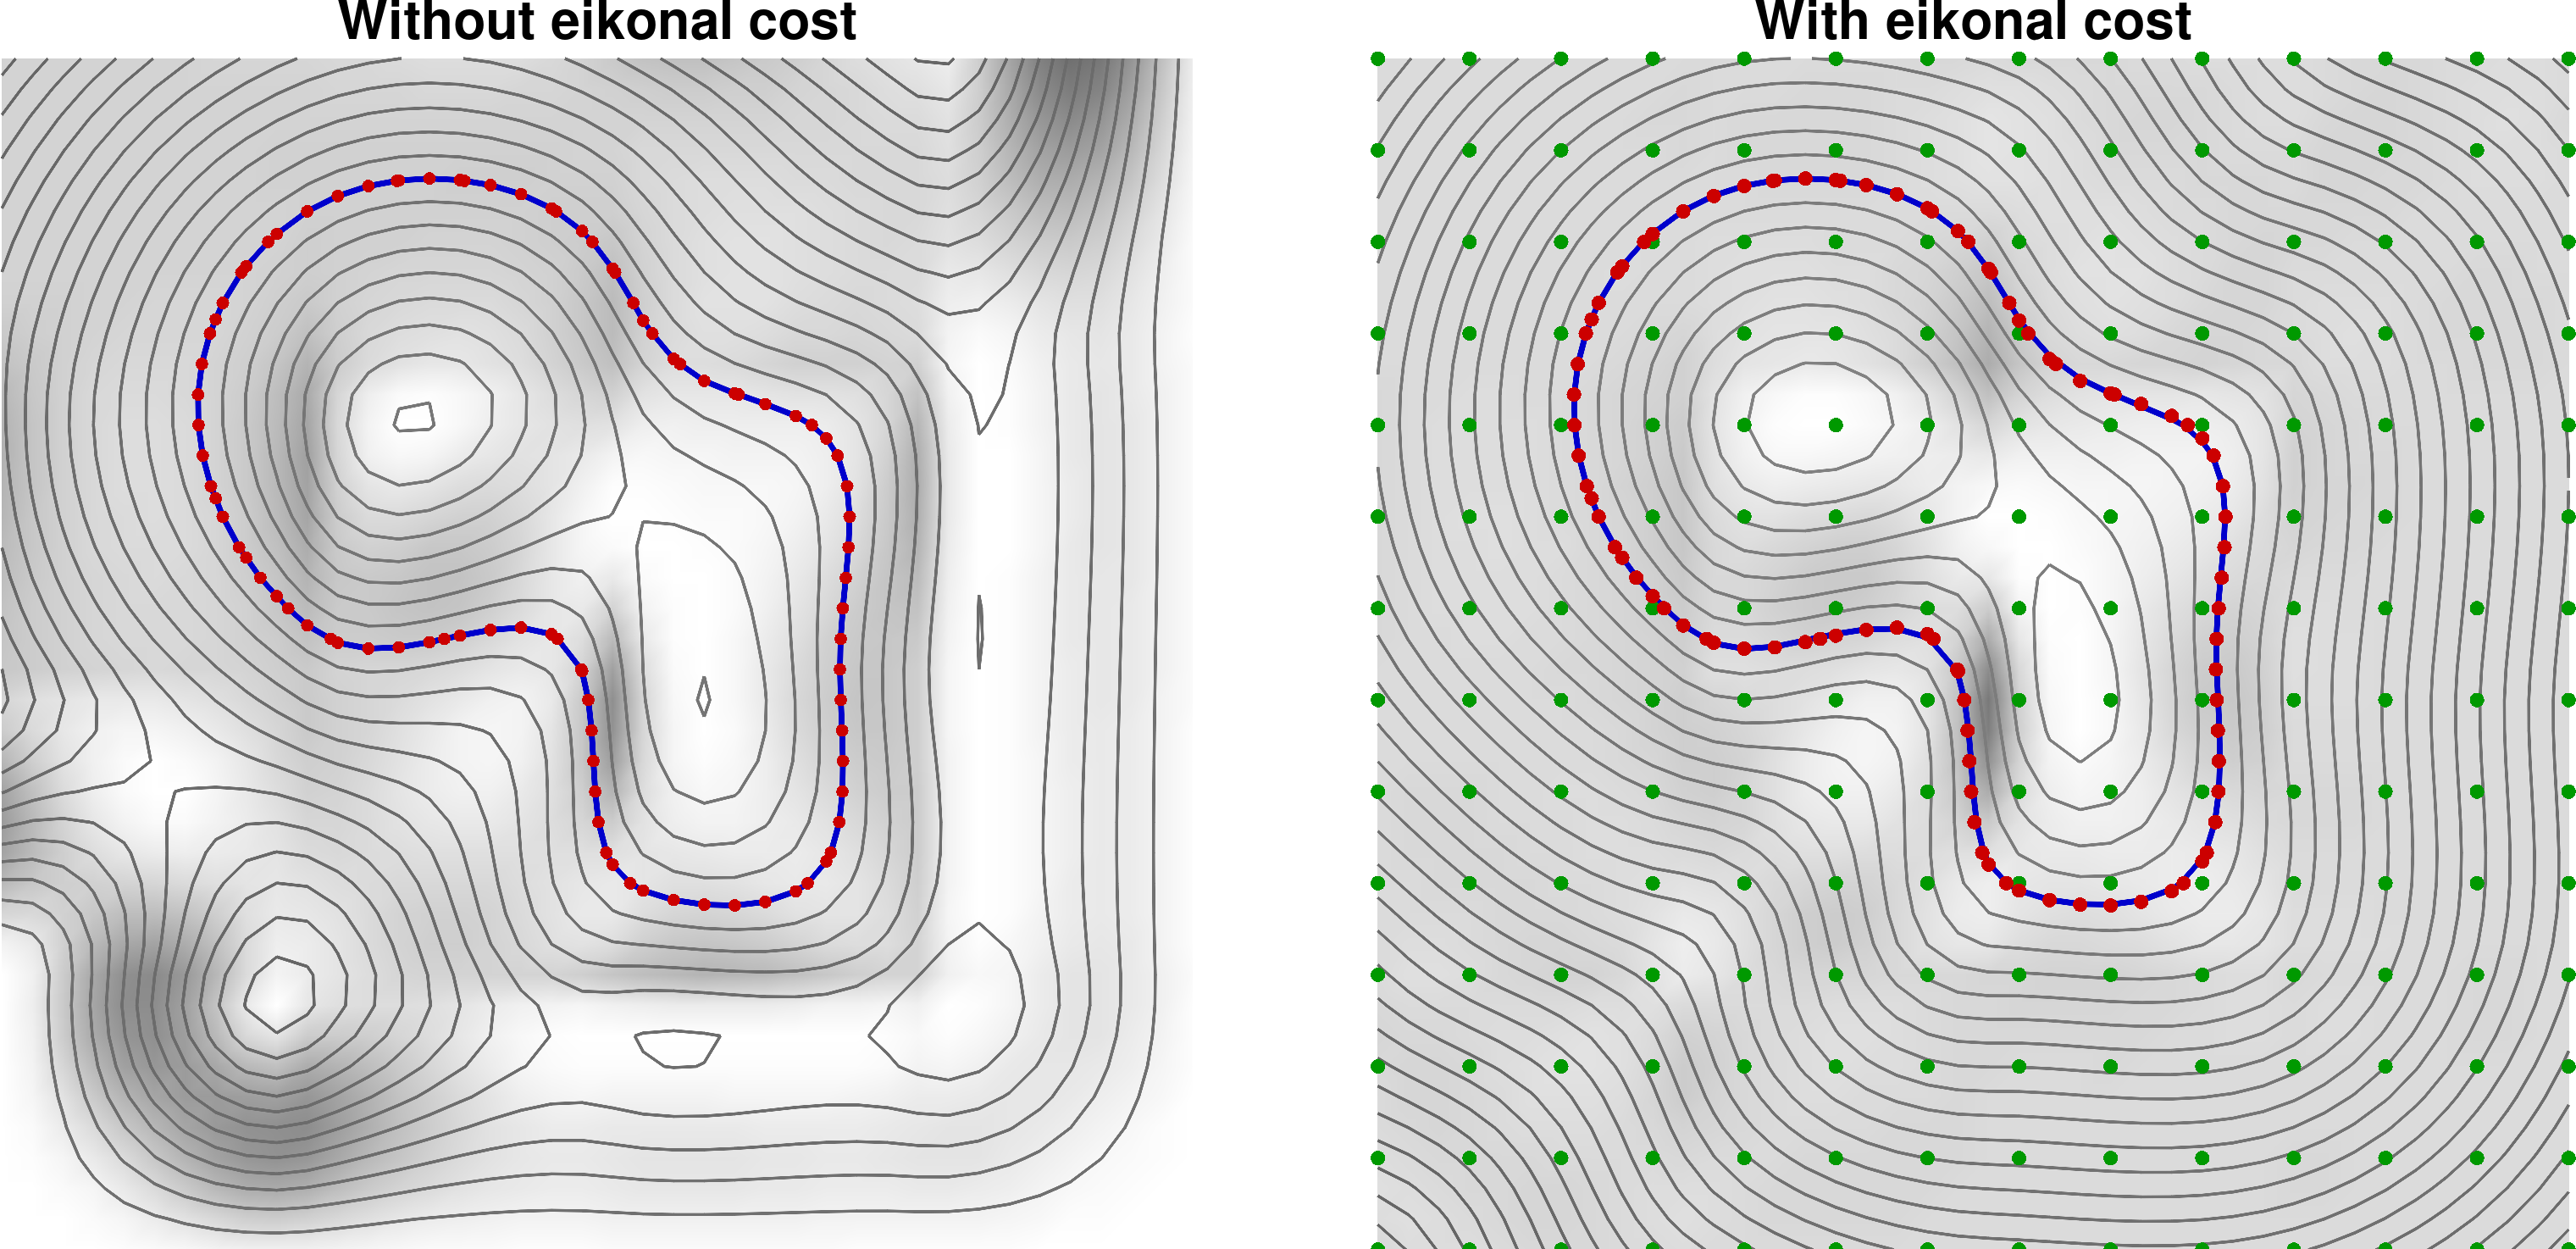
\includegraphics[width=\textwidth]{images/spline2D_eikonal01.png}
%\caption{\footnotesize
%Estimation of an SDF from only contour points (in red), without (left) and with (right) an eikonal cost to privilege a unit norm on the derivatives.
%}
%\label{fig:Bezier_2D_eikonal}
%\end{figure}

\begin{wrapfigure}{r}{.48\textwidth}
%\vspace{-20pt}
\centering
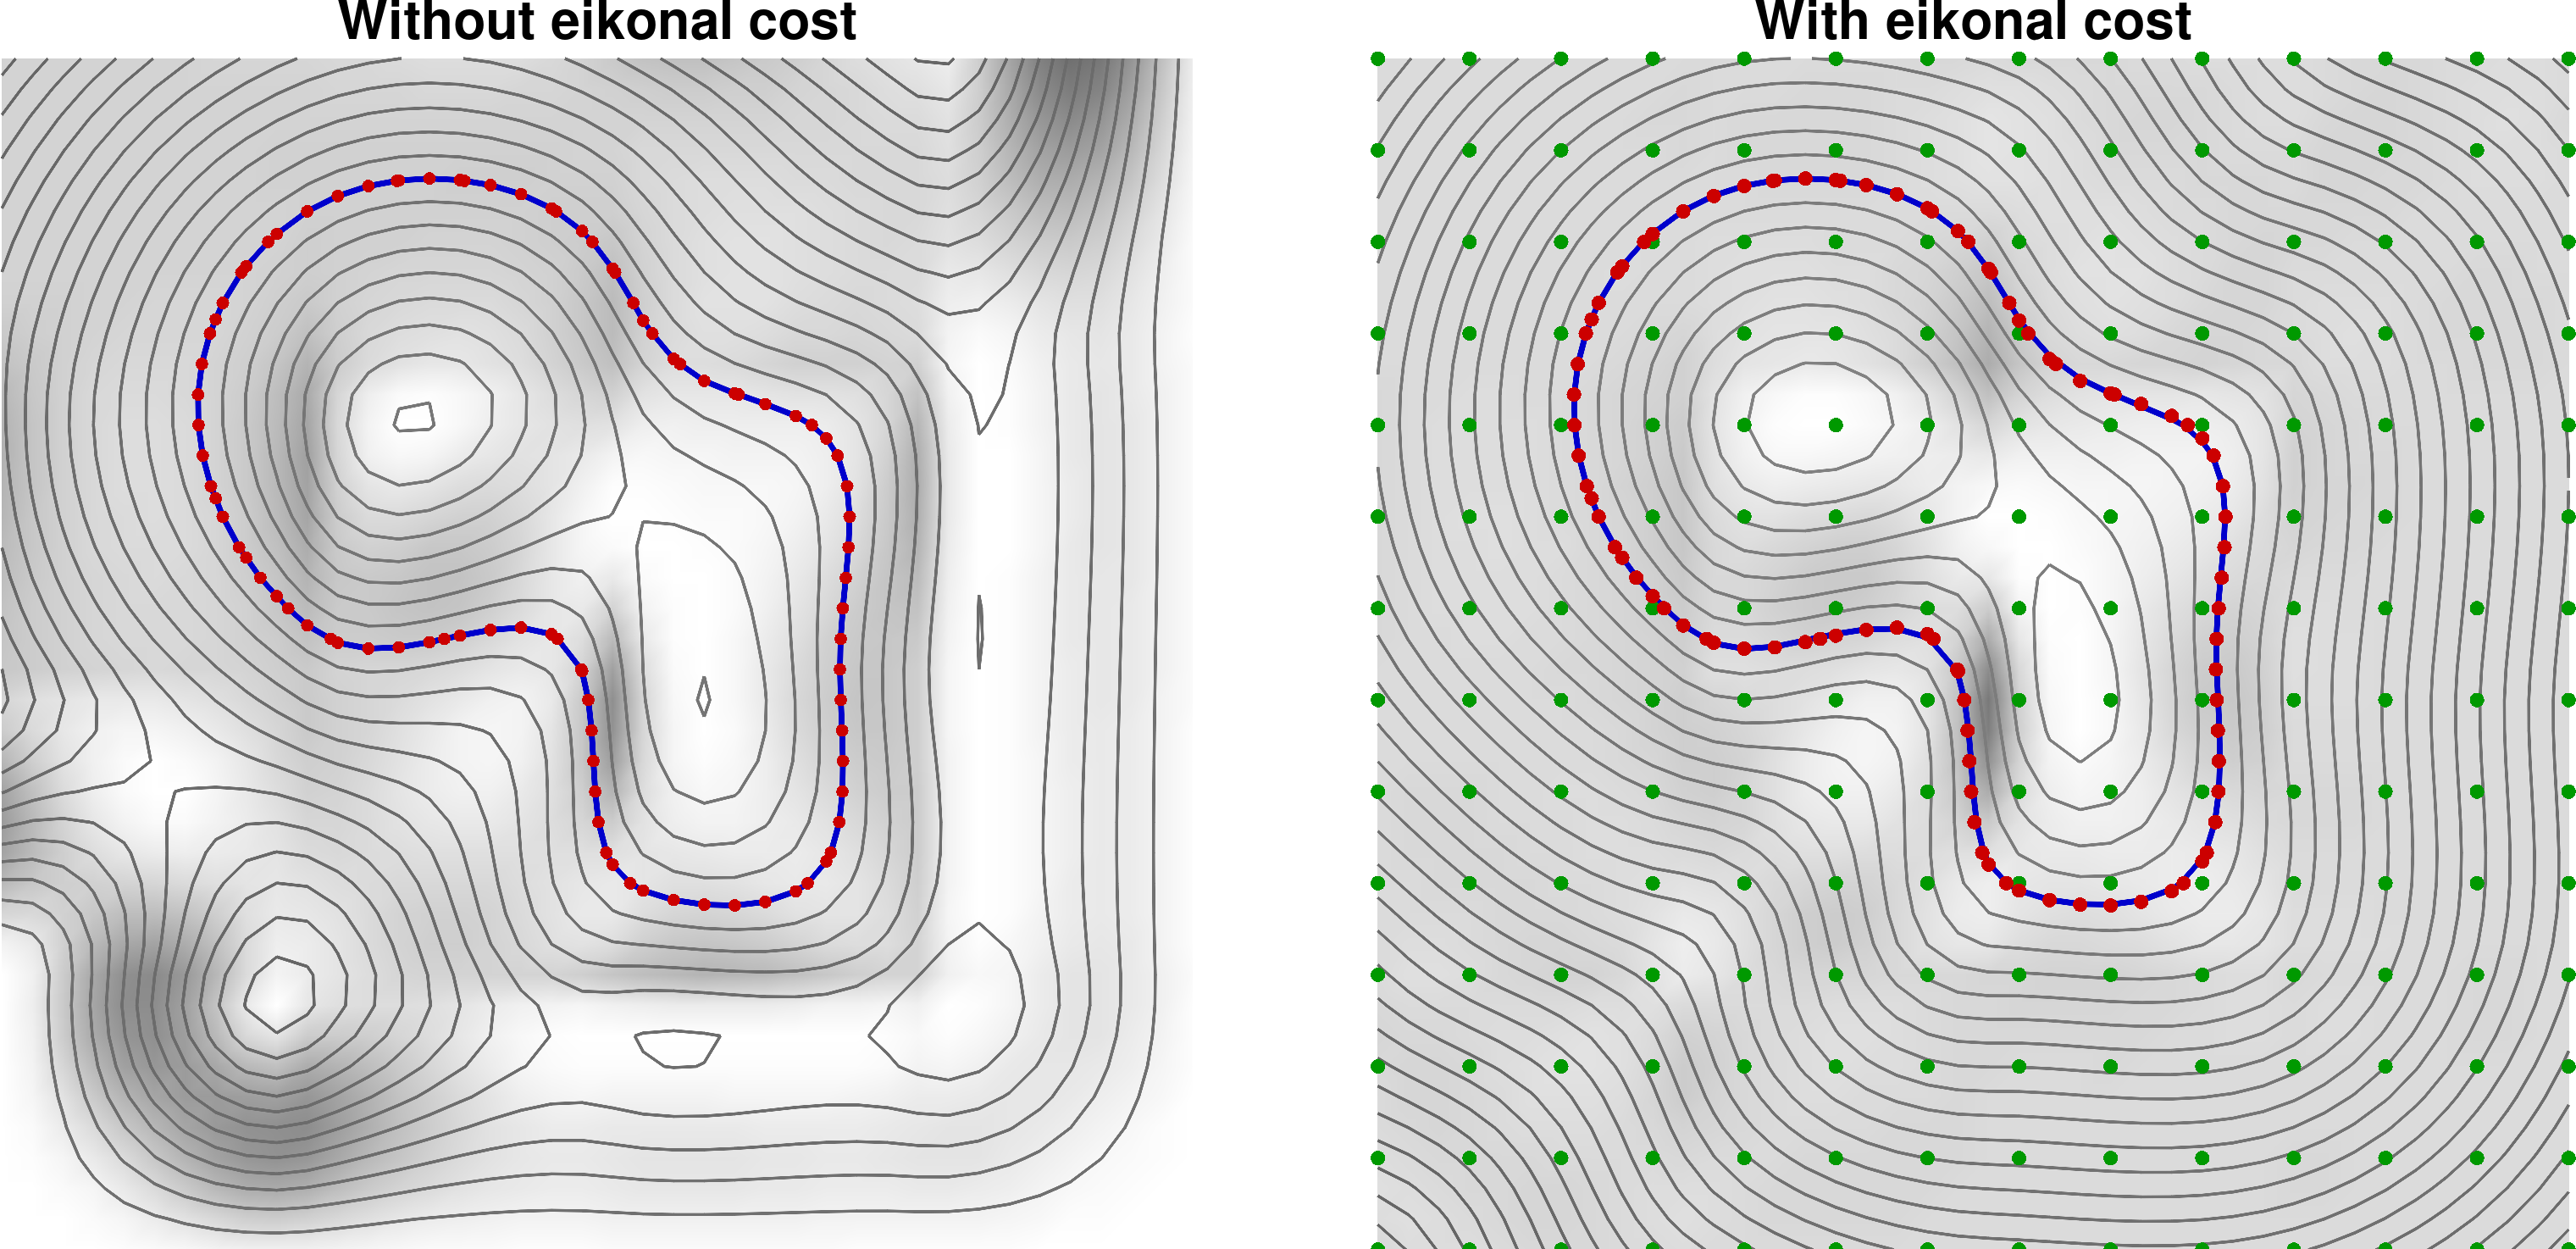
\includegraphics[width=.42\textwidth]{images/spline2D_eikonal01.png}
\caption{\footnotesize
Estimation of an SDF from only contour points (in red), without (\emph{left}) and with (\emph{right}) an eikonal cost to privilege a unit norm on the derivatives. The $M\!=\!93$ points in red are used for the distance matching objective and the $N\!=\!196$ points in green are used for the eikonal objective. The estimated SDFs are rendered as level sets, with the 0-level set (i.e., the contour) in thick blue line. The colormap in the background is proportional to the norm of the gradient, where a homogeneous gray value would mean that the eikonal cost can be satisfied everywhere. Regions with darker or lighter color then correspond to higher eikonal cost. 
}
\label{fig:Bezier_2D_eikonal}
\end{wrapfigure}


We can also estimate an SDF by privileging a unit norm on the derivatives. From a dataset of $M$ distances $x_m$ observed at locations $\bm{t}_m$, the basis functions coefficients $\bm{w}$ of an SDF can be computed by evaluating 
\begin{equation}
	\min_{\bm{w}} \; \sum_{m=1}^M \big\|\bm{\Psi}(\bm{t}_m) \, \bm{w} \, - \, x_m\big\|^2 + 
	\lambda \sum_{n=1}^N \big\|\bm{\nabla}x_n^\trsp \, \bm{\nabla}x_n \, - \, 1 \big\|^2,
	\label{eq:wEikonal}
\end{equation}
where $\lambda$ is a weighting factor balancing the distance matching objective and the eikonal objective (regularization). The gradient of $x_n$ with respect to $\bm{t}$ is expressed as $\bm{\nabla}x_n = \bm{\nabla}\bm{\Psi}(\bm{t}_n) \, \bm{w}$, computed using \eqref{eq:dPsi} for a set of $N$ locations $\bm{t}_n$, that can typically be defined to cover homogeneously the area/volume encoded in the SDF. 

The first component of the objective in \eqref{eq:wEikonal} is to find a SDF that can fit the data. If only this first part would be required, the minimization boils down to the least squares solution of Section \ref{sec:batchSDF}. The second term adds the objective of keeping the norm of the derivatives close to one, which is related to the eikonal equation $\|\bm{\nabla}x\| =1$, see \cite{Gropp20} for the use of the eikonal equation in the context of SDF modeling. Intuitively, as the basis functions encodes a SDF, it means that we expect that if we move away from a shape by a small distance $\Delta d$ in the direction given by the gradient, the expected distance at this new point should also increase by $\Delta d$, which corresponds to a slope of $1$ (namely, a unit norm for the gradient), as expressed in the second part of the objective function.

By following the notation in Section \ref{sec:GaussNewton}, the above objective can be written as a sum of squared functions that can be solved by Gauss--Newton optimization, with residuals and Jacobians given by
\begin{align*}
	r_{1,m} &= \bm{\Psi}(\bm{t}_m) \, \bm{w} - x_m, 
	\quad &
	\bm{J}_{1,m} &= \bm{\Psi}(\bm{t}_m), 
	\quad &
	\forall m\in\{1,\ldots,M\}, 
	\\
	r_{2,n} &= \bm{\nabla}x_n^\trsp \, \bm{\nabla}x_n - 1, 
	\quad & 
	\bm{J}_{2,n} &= 2 \, {\bm{\nabla}x_n}^{\!\trsp} \, \bm{\nabla}\bm{\Psi}(\bm{t}_n), 
	\quad &
	\forall n\in\{1,\ldots,N\},
\end{align*}
which provide at each iteration step $k$ the Gauss--Newton update rule
\begin{equation*}
	\bm{w}_{k+1} \;\leftarrow\; 
	\bm{w}_k - \alpha {\Bigg( \sum_{m=1}^M \bm{J}_{1,m}^\trsp \bm{J}_{1,m} + \lambda \sum_{n=1}^N \bm{J}_{2,n}^\trsp \bm{J}_{2,n} \Bigg)}^{\!-1} \, 
	\Bigg( \sum_{m=1}^M \bm{J}_{1,m}^\trsp \, r_{1,m} + \lambda \sum_{n=1}^N \bm{J}_{2,n}^\trsp \, r_{2,n} \bigg),\\
\end{equation*}
as detailed in Section \ref{sec:GaussNewton}, where the learning rate $\alpha$ can be determined by line search.

Note that the above computation can be rewritten with concatenated vectors and matrices for more efficient computation exploiting linear algebra. By concatenating vertically the Jacobian matrices and residuals, we have the equivalent Gauss--Newton update rule
\begin{equation*}
	\bm{w}_{k+1} \;\leftarrow\; 
	\bm{w}_k - \alpha {\Bigg( \bm{J}_{1}^\trsp \bm{J}_{1} + \lambda \bm{J}_{2}^\trsp \bm{J}_{2} \Bigg)}^{\!-1} \, 
	\Bigg( \bm{J}_{1}^\trsp \, \bm{r}_{1} + \lambda \bm{J}_{2}^\trsp \, \bm{r}_{2} \bigg).
\end{equation*}

Figure \ref{fig:Bezier_2D_eikonal} presents an example in 2D.


%%%%%%%%%%%%%%%%%%%%%%%%%%%%%%%%%%%%%%%%%%%%%%%%%%%%%%%%%%%%%%%%%%%%%%%%%%%%%%%%%
\section{Linear quadratic tracking (LQT)}\label{sec:LQT}
\begin{flushright}
\filename{LQT.*}
\end{flushright}

Linear quadratic tracking (LQT) is a simple form of optimal control that trades off tracking and control costs expressed as quadratic terms over a time horizon, with the evolution of the state described in a linear form. The LQT problem is formulated as the minimization of the cost
\begin{align}
	c
	&= {\big(\bm{\mu}_T\!-\!\bm{x}_T\big)}^\trsp
	\bm{Q}_T 
	\big(\bm{\mu}_T\!-\!\bm{x}_T\big) +
	\sum_{t=1}^{T-1} \Big({\big(\bm{\mu}_t\!-\!\bm{x}_t\big)}^\trsp
	\bm{Q}_t  
	\big(\bm{\mu}_t\!-\!\bm{x}_t\big) 
	\;+\;
	\bm{u}_t^\trsp \bm{R}_t\; \bm{u}_t \Big)
	\nonumber\\
	&= {\big(\bm{\mu}-\bm{x}\big)}^\trsp
	\bm{Q} 
	\big(\bm{\mu}-\bm{x}\big)
	\;+\;
	\bm{u}^\trsp \!\bm{R} \bm{u} ,
	\label{eq:cBatch}
\end{align}
with $\bm{x}\!=\!{\begin{bmatrix}\bm{x}_1^\trsp, \bm{x}_2^\trsp, \ldots, \bm{x}_T^\trsp \end{bmatrix}}^\trsp$ the evolution of the state variables, 
$\bm{u}\!=\!{\begin{bmatrix}\bm{u}_1^\trsp, \bm{u}_2^\trsp, \ldots, \bm{u}_{T-1}^\trsp \end{bmatrix}}^\trsp$ the evolution of the control commands, and 
$\bm{\mu}\!=\!{\begin{bmatrix}\bm{\mu}_1^\trsp, \bm{\mu}_2^\trsp, \ldots, \bm{\mu}_T^\trsp \end{bmatrix}}^\trsp$ the evolution of the tracking targets.
$\bm{Q}\!=\!\mathrm{blockdiag}(\bm{Q}_1,\bm{Q}_2,\ldots,\bm{Q}_T)$ represents the evolution of the precision matrices $\bm{Q}_t$, and 
$\bm{R}\!=\!\mathrm{blockdiag}(\bm{R}_{1},\bm{R}_{2},\ldots,\bm{R}_{T-1})$ represents the evolution of the control weight matrices $\bm{R}_t$. 

The evolution of the system is linear, described by 
\begin{equation}
	\bm{x}_{t+1} = \bm{A}_t \bm{x}_t + \bm{B}_t \bm{u}_t, 
	\label{eq:linSys}
\end{equation}
yielding at trajectory level
\begin{equation}
	\bm{x} = \bm{S}_{\bm{x}} \bm{x}_1 + \bm{S}_{\bm{u}} \bm{u}, 
	\label{eq:linSysTraj}
\end{equation}
see Appendix \ref{app:Su} for details.

With open loop control commands organized as a vector $\bm{u}$, the solution of \eqref{eq:cBatch} subject to $\bm{x}=\bm{S}_{\bm{x}}\bm{x}_1+\bm{S}_{\bm{u}}\bm{u}$ is analytic, given by
\begin{equation}
	\bm{\hat{u}} = {\big(\bm{S}_{\bm{u}}^\trsp \bm{Q} \bm{S}_{\bm{u}} + \bm{R}\big)}^{-1}
	\bm{S}_{\bm{u}}^\trsp \bm{Q} 
	\big(\bm{\mu} - \bm{S}_{\bm{x}} \bm{x}_1 \big).
	\label{eq:uLQT}
\end{equation}

The residuals of this least squares solution provides information about the uncertainty of this estimate, in the form of a full covariance matrix (at control trajectory level)
\begin{equation}
	\bm{\hat{\Sigma}}^{\bm{u}} = {\big(\bm{S}_{\bm{u}}^\trsp \bm{Q} \bm{S}_{\bm{u}} + \bm{R}\big)}^{-1},
	\label{eq:uSigma}
\end{equation}
which provides a probabilistic interpretation of LQT, see Section \ref{sec:PoG}.

The batch computation approach facilitates the creation of bridges between learning and control. For example, in learning from demonstration, the observed (co)variations in a task can be formulated as an LQT objective function, which then provides a trajectory distribution in control space that can be converted to a trajectory distribution in state space. All the operations are analytic and only exploit basic linear algebra.

The approach can also be extended to model predictive control (MPC), iterative LQR (iLQR) and differential dynamic programming (DDP), whose solution needs this time to be interpreted locally at each iteration step of the algorithm, as we will see later in the technical report.

%\!\in\!\mathbb{R}^{DCT} 
%\!\in\!\mathbb{R}^{d(T-1)} 
%\!\in\!\mathbb{R}^{DCT}
%\in\mathbb{R}^{d(T-1)\times d(T-1)}
%\in\mathbb{R}^{DCT\times DCT}


%%%%%%%%%%%%%%%%%%%%%%%%%%%%%%%%%%%%%%%%%%%%%%%%%%%%%%%%%%%%%%%%%%%%%%%%%%%%%%%%%
\subsubsection*{Example: Bimanual tennis serve}
\begin{flushright}
\filename{LQT\_tennisServe.*}
\end{flushright}

\begin{figure}
\centering
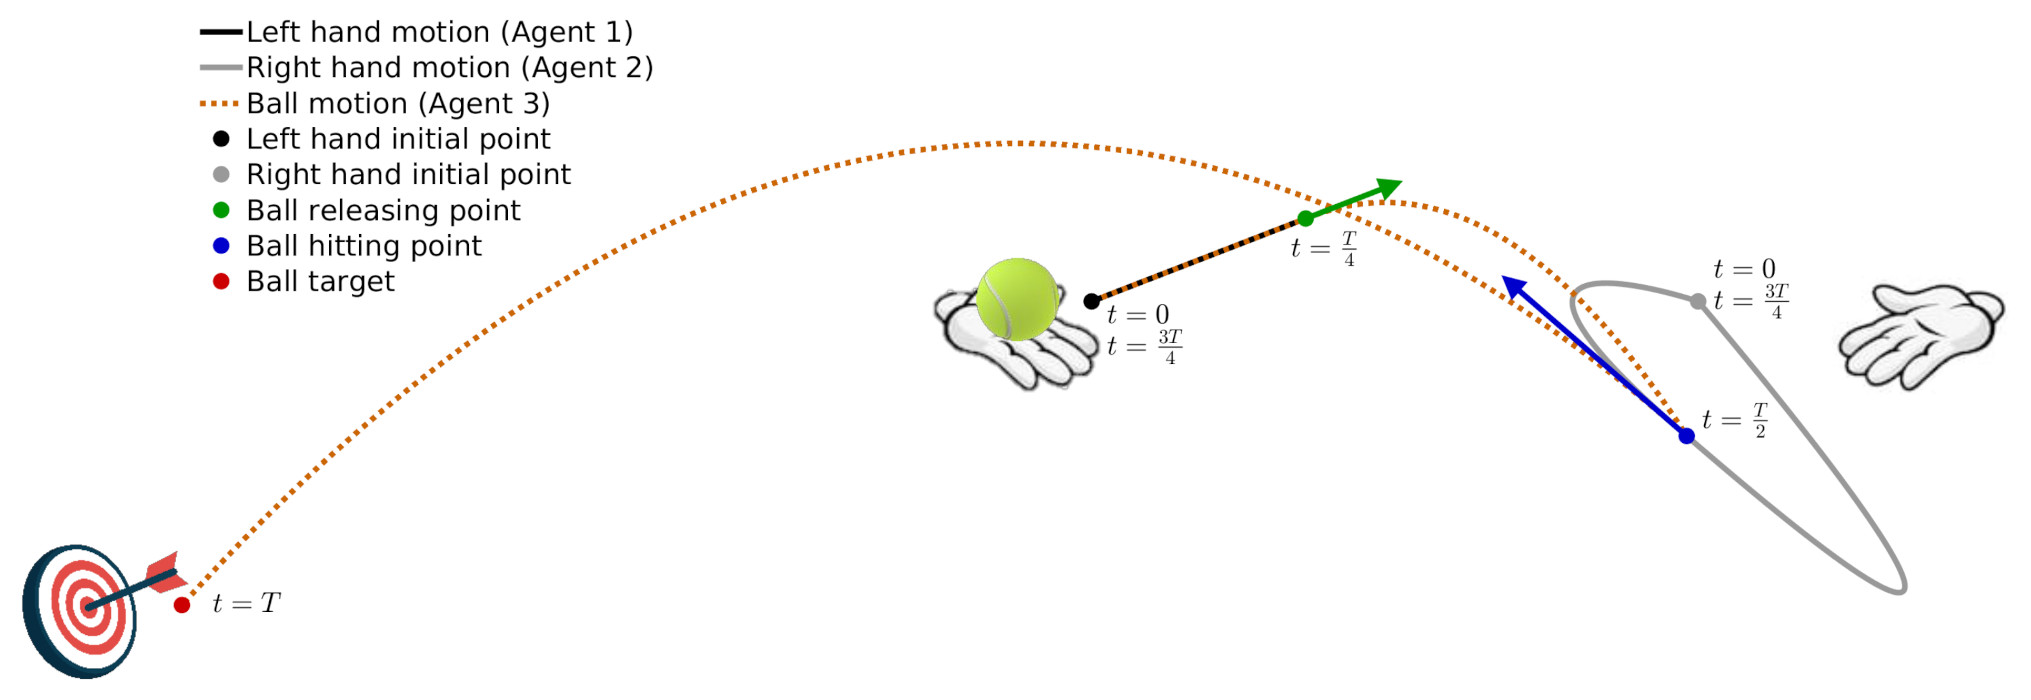
\includegraphics[width=.7\columnwidth]{images/LQT_tennisServe01.jpg}
\caption{\footnotesize
Tennis serve problem solved by linear quadratic tracking (LQT).
}
\label{fig:LQT_tennis}
\end{figure}

LQT can be used to solve a ballistic task mimicking a bimanual tennis serve problem. In this problem, a ball is thrown by one hand and then hit by the other, with the goal of bringing the ball to a desired target, see Fig.~\ref{fig:LQT_tennis}. 
The problem is formulated as in \eqref{eq:cBatch}, namely 
\begin{equation}
	\min_{\bm{u}} {(\bm{\mu}-\bm{x})}^{\!\trsp}
	\bm{Q} 
	(\bm{\mu}-\bm{x})
	\;+\;
	\bm{u}^{\!\trsp} \!\bm{R} \bm{u},
	\;\text{s.t.}\;
	\bm{x}=\bm{S}_{\bm{x}}\bm{x}_1+\bm{S}_{\bm{u}}\bm{u},
	\label{eq:cTennis}
\end{equation}
where $\bm{x}$ represents the state trajectory of the 3 agents (left hand, right hand and ball), where only the hands can be controlled by a series of acceleration commands $\bm{u}$ that can be estimated by LQT.

In the above problem, $\bm{Q}$ is a precision matrix and $\bm{\mu}$ is a reference vector describing at specific time steps the targets that the three agents must reach. The linear systems are described according to the different phases of the task, see Appendix \ref{app:tennis} for details. As shown above, the constrained objective in \eqref{eq:cTennis} can be solved by least squares, providing an analytical solution given by \eqref{eq:uLQT}, see also Fig.~\ref{fig:LQT_tennis} for the visualization of the result for a given target and for given initial poses of the hands.


%%%%%%%%%%%%%%%%%%%%%%%%%%%%%%%%%%%%%%%%%%%%%%%%%%%%%%%%%%%%%%%%%%%%%%%%%%%%%%%%%
\subsection{LQT with smoothness cost}
\begin{flushright}
\filename{LQT.*}
\end{flushright}

%\begin{figure}
%\centering
%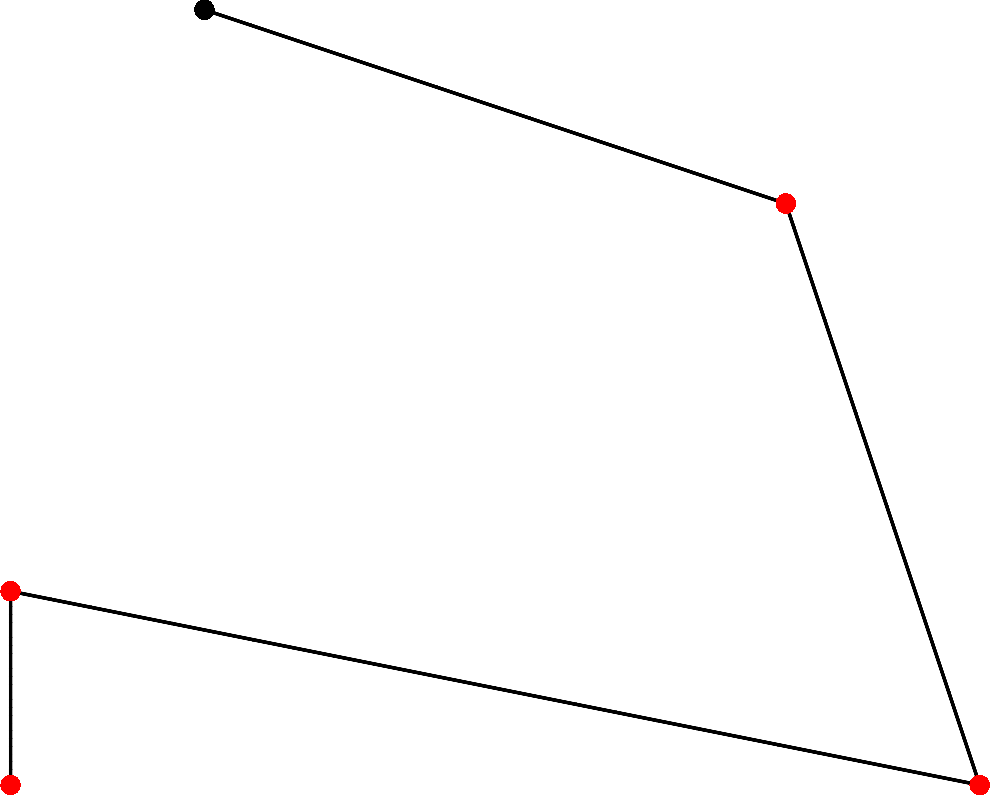
\includegraphics[width=.32\columnwidth]{images/LQT_smooth01.png}
%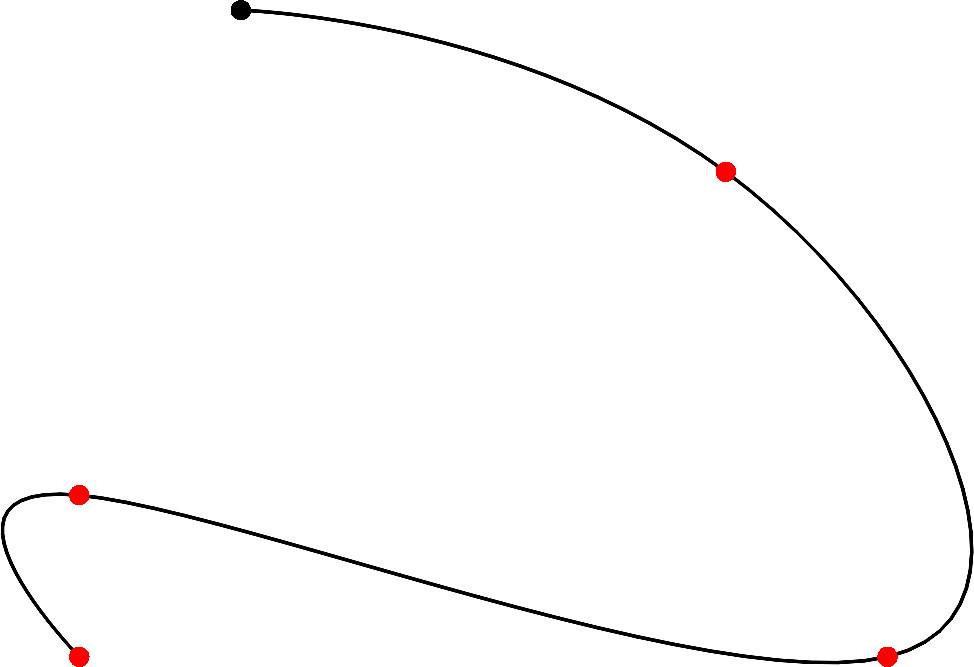
\includegraphics[width=.32\columnwidth]{images/LQT_smooth02.png}
%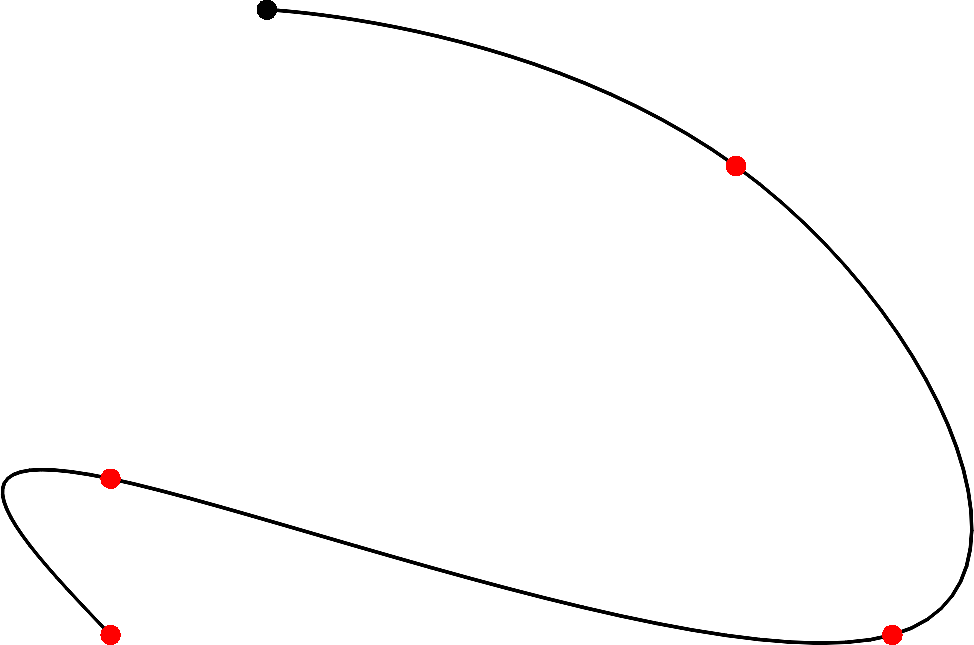
\includegraphics[width=.32\columnwidth]{images/LQT_smooth03.png}
%\caption{\footnotesize
%Examples of linear quadratic tracking (LQT) applied to the task of reaching a set of viapoints (red dots) by starting from an initial position (black dot). \emph{Left:} With velocity commands, with a system described as a single integrator and a standard control cost. \emph{Center:} With velocity commands, with a system described as a single integrator and a control cost ensuring smoothness. \emph{Right:} With acceleration commands, with a system described as a double integrator and a standard control cost.
%}
%\label{fig:LQT_smooth}
%\end{figure}

\begin{wrapfigure}{r}{.42\textwidth}
\vspace{-20pt}
\centering
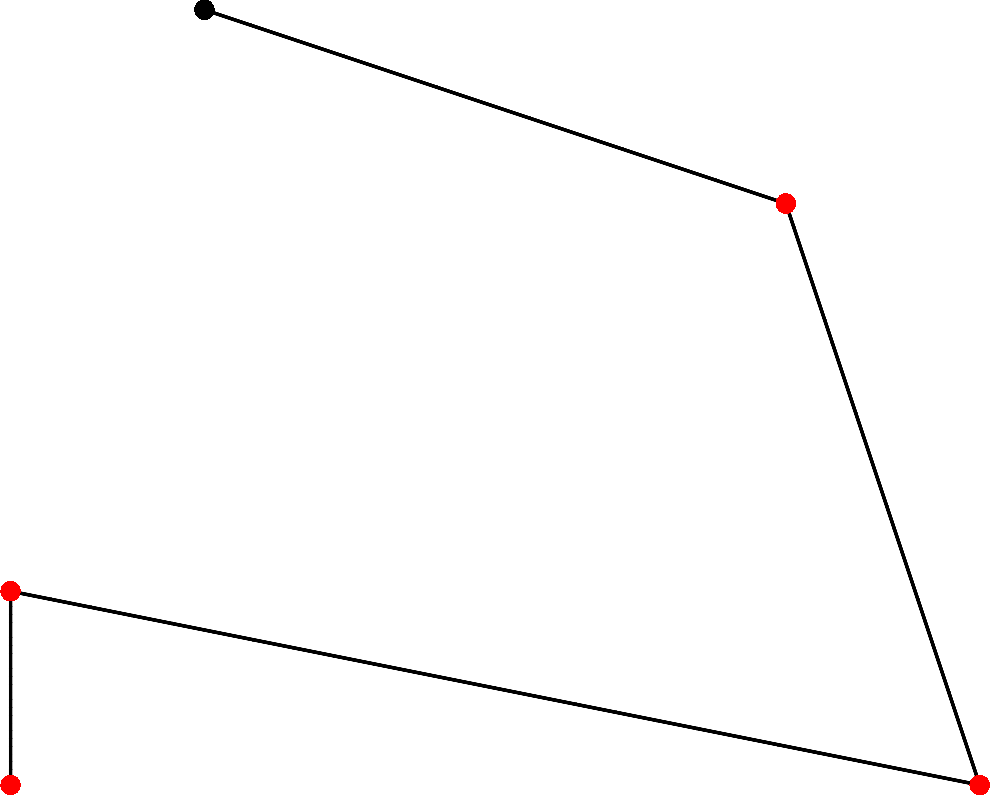
\includegraphics[width=.14\columnwidth]{images/LQT_smooth01.png}\hspace{8mm}
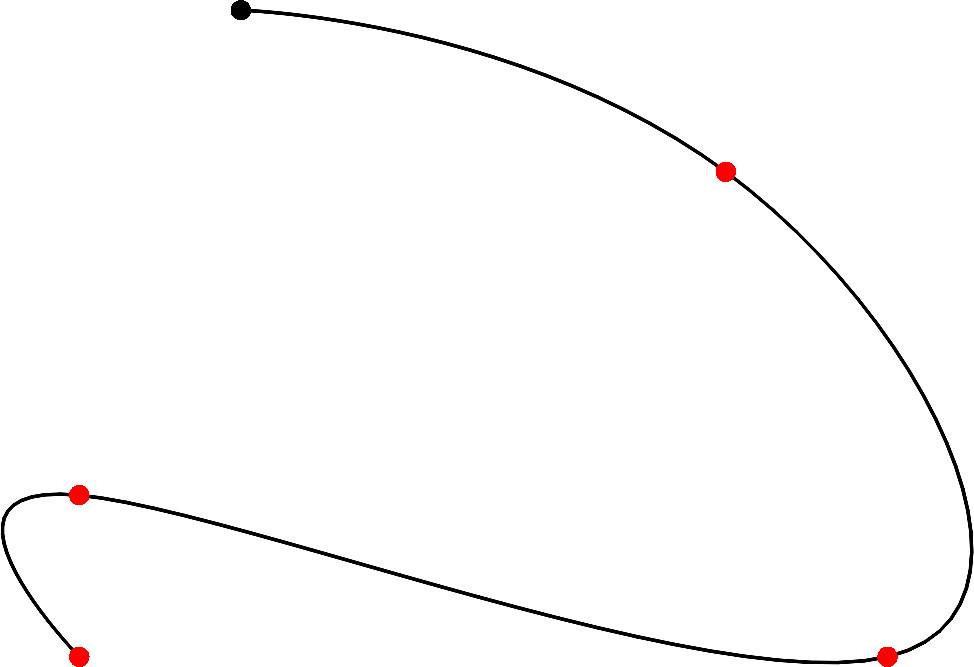
\includegraphics[width=.14\columnwidth]{images/LQT_smooth02.png}\\[8mm]
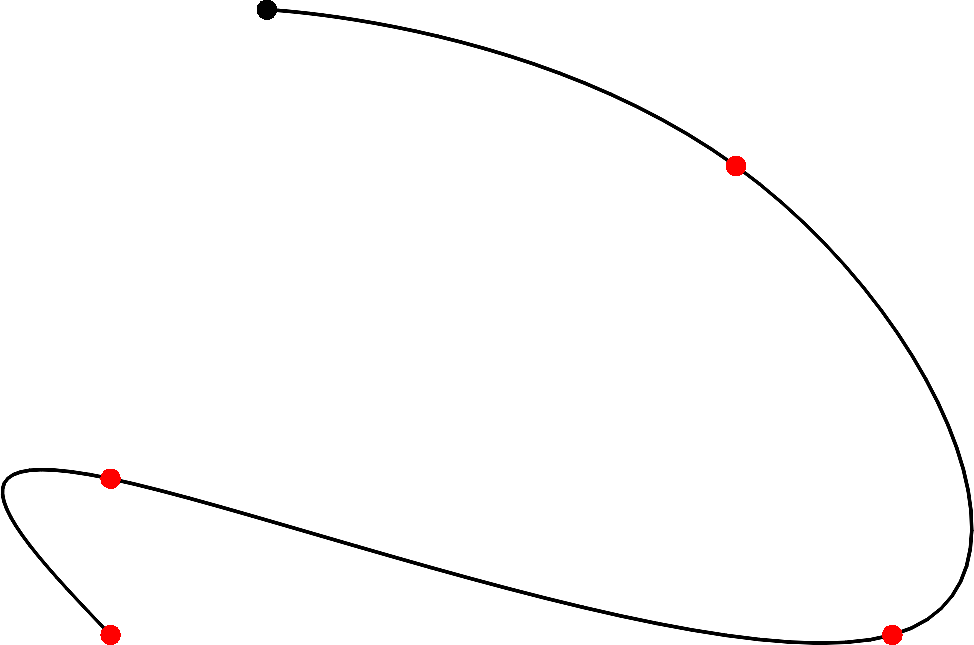
\includegraphics[width=.14\columnwidth]{images/LQT_smooth03.png}
\caption{\footnotesize
Examples of linear quadratic tracking (LQT) applied to the task of reaching a set of viapoints (red dots) by starting from an initial position (black dot). \emph{Top-left:} With velocity commands, with a system described as a single integrator and a standard control cost. \emph{Top-right:} With velocity commands, with a system described as a single integrator and a control cost ensuring smoothness. \emph{Bottom:} With acceleration commands, with a system described as a double integrator and a standard control cost.
}
\label{fig:LQT_smooth}
%\vspace{-40pt}
\end{wrapfigure}

Linear quadratic tracking (LQT) can be used with dynamical systems described as simple integrators. With single integrators, the states correspond to positions, with velocity control commands. With double integrators, the states correspond to positions and velocities, with acceleration control commands. With triple integrators, the states correspond to positions, velocities and accelerations, with jerk control commands, etc.

Figure \ref{fig:LQT_smooth} shows an example of LQT for a task that consist of passing through a set of viapoints. The left and right graphs show the result for single and double integrators, respectively. The graph in the center also considers a single integrator, by redefining the weight matrix $\bm{R}$ of the control cost to ensure smoothness. This can be done by replacing the standard diagonal $\bm{R}$ matrix in \eqref{eq:cBatch} with
\begin{equation*}
	\bm{R} = \left[\begin{matrix}
	 2 & -1 &  0 &  0 & \cdots & 0 & 0 \\
	-1 &  2 & -1 &  0 & \cdots & 0 & 0 \\
	 0 & -1 &  2 & -1 & \cdots & 0 & 0 \\
	\vdots & \vdots & \vdots & \vdots & \ddots & \vdots & \vdots \\
	 0 &  0 &  0 &  0 & \cdots &  2 & -1 \\
	 0 &  0 &  0 &  0 & \cdots & -1 &  2 
	\end{matrix}\right] 
	\otimes \bm{I}_D.
\end{equation*}
%e = ones(param.nbData-1,1) * param.r;
%R = kron(spdiags([-e 2*e -e], -1:1, param.nbData-1, param.nbData-1), speye(param.nbVarPos)); %Control weight matrix as transition matrix to encourage smoothness
\newline

\newpage
%%%%%%%%%%%%%%%%%%%%%%%%%%%%%%%%%%%%%%%%%%%%%%%%%%%%%%%%%%%%%%%%%%%%%%%%%%%%%%%%%
\subsection{LQT with control primitives}
\begin{flushright}
\filename{LQT\_CP.*}
\end{flushright}

If we assume that the control commands profile $\bm{u}$ is composed of \emph{control primitives} (CP) with $\bm{u}=\bm{\Psi}\bm{w}$, the objective becomes
\begin{equation*}
	\min_{\bm{w}} {(\bm{x}-\bm{\mu})}^{\!\trsp}
	\bm{Q} 
	(\bm{x}-\bm{\mu})
	\;+\;
	\bm{w}^{\!\trsp} \bm{\Psi}^{\!\trsp} \bm{R} \bm{\Psi} \bm{w},
	\quad\text{s.t.}\quad
	\bm{x}=\bm{S}_{\bm{x}}\bm{x}_1+\bm{S}_{\bm{u}} \bm{\Psi} \bm{w},
\end{equation*}
with a solution given by
\begin{equation*}
	\bm{\hat{w}} = {\big(\bm{\Psi}^{\!\trsp}  \bm{S}_{\bm{u}}^\trsp \bm{Q} \bm{S}_{\bm{u}} \bm{\Psi} + \bm{\Psi}^{\!\trsp} \bm{R} \bm{\Psi}  \big)}^{-1}
	\bm{\Psi}^{\!\trsp} \bm{S}_{\bm{u}}^\trsp \bm{Q} \big(\bm{\mu} - \bm{S}_{\bm{x}} \bm{x}_1 \big),
\end{equation*}
which is used to compute the trajectory $\bm{\hat{u}}=\bm{\Psi}\bm{\hat{w}}$ in control space, corresponding to the list of control commands organized in vector form. Similarly to \eqref{eq:uSigma}, the residuals of the least squares solution provides a probabilistic approach to LQT with control primitives. Note also that the trajectory in control space can be converted to a trajectory in state space with $\bm{\hat{x}}=\bm{S}_{\bm{x}}\bm{x}_1+\bm{S}_{\bm{u}}\bm{\hat{u}}$. Thus, since all operations are linear, a covariance matrix on $\bm{w}$ can be converted to a covariance on $\bm{u}$ and on $\bm{x}$. A similar linear transformation is used in the context of probabilistic movement primitives (ProMP) \cite{Paraschos13} to map a covariance matrix on $\bm{w}$ to a covariance on $\bm{x}$. LQT with control primitives provides a more general approach by considering both control and state spaces. It also has the advantage of reframing the method to the more general context of optimal control, thus providing various extension opportunities.

Several forms of basis functions can be considered, including stepwise control commands, radial basis functions (RBFs), Bernstein polynomials, Fourier series, or learned basis functions, which are organized as a dictionary matrix $\bm{\Psi}$. Dictionaries for multivariate control commands can be generated with a Kronecker product operator $\otimes$ as
\begin{equation} 
	\bm{\Psi} = \bm{\phi} \otimes \bm{C},
	\label{eq:Psi2}
\end{equation}
where the matrix $\bm{\phi}$ is a horizontal concatenation of univariate basis functions, and $\bm{C}$ is a coordination matrix, which can be set to an identity matrix $\bm{I}_D$ for the generic case of control variables with independent basis functions for each dimension $d\in\{1,\ldots,D\}$.

Note also that in some situations, $\bm{R}$ can be set to zero because the regularization role of $\bm{R}$ in the original problem formulation can sometimes be redundant with the use of sparse basis functions.


%%%%%%%%%%%%%%%%%%%%%%%%%%%%%%%%%%%%%%%%%%%%%%%%%%%%%%%%%%%%%%%%%%%%%%%%%%%%%%%%%
\subsection{LQR with a recursive formulation}\label{sec:LQRrecursive}
\begin{flushright}
\filename{LQT\_recursive.*}
\end{flushright}
%See also Borrelli's book (2015), or Boyd's lecture notes (https://stanford.edu/class/ee363/lectures/dlqr.pdf)

\begin{algorithm}
\caption{Recursive formulation of LQR}
\label{alg:LQRrecursive}
Define quadratic cost function with $\bm{Q}_t$, $\bm{R}_t$ \\ 
Define dynamics with $\bm{A}_t$, $\bm{B}_t$, and initial state $\bm{x}_1$ \\
\tcp{Backward pass} 
Set $\bm{V}_T=\bm{Q}_T$ \\
\For{$t \gets T-1$ to $1$}{
	Compute $\bm{V}_t$ with \eqref{eq:V} and \eqref{eq:ct1}
}
\tcp{Forward pass} 
\For{$t \gets 1$ to $T-1$}{
	Compute $\bm{K}_t$ and $\bm{\hat{u}}_t$ with \eqref{eq:uLQRrecursive} \\
	Compute $\bm{x}_{t+1}$ with \eqref{eq:linSys}
}
\end{algorithm}

The LQR problem is formulated as the minimization of the cost
\begin{equation}
	c(\bm{x}_1,\bm{u}) = c_T(\bm{x}_T) + \sum_{t=1}^{T-1} c_t(\bm{x}_t,\bm{u}_t) 
	\;= \bm{x}_T^\trsp \bm{Q}_T \bm{x}_T + 
	\sum_{t=1}^{T-1} \Big(\bm{x}_t^\trsp \bm{Q}_t \bm{x}_t +
	\bm{u}_t^\trsp \bm{R}_t \, \bm{u}_t \Big), 
	\quad\text{s.t.}\quad 
	\bm{x}_{t+1} = \bm{A}_t \bm{x}_{t} + \bm{B}_t \bm{u}_{t},
\label{eq:cLQR}
\end{equation}
where $c$ without index refers to the total cost (cumulative cost). 
We also define the partial cumulative cost 
\begin{equation}
	v_t(\bm{x}_t,\bm{u}_{t:T-1}) = c_T(\bm{x}_T) + \sum_{s=t}^{T-1} c_s(\bm{x}_t,\bm{u}_t),
	\label{eq:cumulativeCost}
\end{equation}
which depends on the states and control commands, except for $v_T$ that only depends on the state. 

We define the \emph{value function} as the value taken by $v_t$ when applying optimal control commands, namely
\begin{equation}
	\hat{v}_t(\bm{x}_t) = \min_{\bm{u}_{t:T-1}} v_t(\bm{x}_t,\bm{u}_{t:T-1}).
	\label{eq:valueFunction}
\end{equation}

We will use the dynamic programming principle to reduce the minimization in \eqref{eq:valueFunction} over the entire sequence of control commands $\bm{u}_{t:T-1}$ to a sequence of minimization problems over control commands at a single time step, by proceeding backwards in time. 

By inserting \eqref{eq:cumulativeCost} in \eqref{eq:valueFunction}, we observe that
\begin{align}
	\hat{v}_t(\bm{x}_t) &= \min_{\bm{u}_{t:T-1}} \Big( c_T(\bm{x}_T) + \sum_{s=t}^{T-1} c_s(\bm{x}_t,\bm{u}_t) \Big) \nonumber\\
	&= \min_{\bm{u}_t} c_t(\bm{x}_t,\bm{u}_t) \! + 
	\!\!\! \min_{\bm{u}_{t+1:T-1}} \!\!\! \Big( \! c_T(\bm{x}_T) \! + \!\! \sum_{s=t+1}^{T-1} \!\! c_s(\bm{x}_t,\bm{u}_t) \! \Big) \nonumber\\
	&= \min_{\bm{u}_t} \underbrace{c_t(\bm{x}_t,\bm{u}_t) + \hat{v}_{t+1}(\bm{x}_{t+1})}_{q_t(\bm{x}_t,\bm{u}_t)},
	\label{eq:qtLQR}
\end{align}
where $q_t$ is called the \emph{q-function}.

%Since $\hat{v}_T(\bm{x}_T) = c_T(\bm{x}_T)$ is independent of the control commands, we will show that we can compute $\hat{v}_t$ by backward recursion from $t=T-1$ to $t=1$.

By starting from the last time step $T$, and by relabeling $\bm{Q}_T$ as $\bm{V}_T$, we can see that $\hat{v}_T(\bm{x}_T) = c_T(\bm{x}_T)$ is independent of the control commands, taking the quadratic error form
\begin{equation}
	\hat{v}_{T} = \bm{x}_T^\trsp \bm{V}_T \bm{x}_T,
	\label{eq:vhatT}
\end{equation}
which only involves the final state $\bm{x}_T$. We will show that $\hat{v}_{T-1}$ has the same quadratic form as $\hat{v}_{T}$, enabling the backward recursive computation of $\hat{v}_{t}$ from $t=T-1$ to $t=1$.

With \eqref{eq:qtLQR}, the dynamic programming recursion takes the form 
\begin{equation}
	\hat{v}_t = \min_{\bm{u}_t} 
	\begin{bmatrix} \bm{x}_t \\ \bm{u}_t \end{bmatrix}^\trsp
	\begin{bmatrix} \bm{Q}_t & \bm{0} \\ \bm{0} & \bm{R}_t \end{bmatrix}
	\begin{bmatrix} \bm{x}_t \\ \bm{u}_t \end{bmatrix}
	+ 
	\bm{x}_{t+1}^\trsp \bm{V}_{t+1} \bm{x}_{t+1}.
	\label{eq:ct0}
\end{equation}

By substituting $\bm{x}_{{t+1}}=\bm{A}_t\bm{x}_t+\bm{B}_t\bm{u}_t$ into \eqref{eq:ct0}, $\hat{v}_t$ can be rewritten as
\begin{equation}
	\hat{v}_t = \min_{\bm{u}_t} 
	\begin{bmatrix} \bm{x}_t \\ \bm{u}_t \end{bmatrix}^\trsp
	\begin{bmatrix} \bm{Q}_{\bm{x}\bm{x},t} & \bm{Q}_{\bm{u}\bm{x},t}^\trsp \\ \bm{Q}_{\bm{u}\bm{x},t} & \bm{Q}_{\bm{u}\bm{u},t} \end{bmatrix}
	\begin{bmatrix} \bm{x}_t \\ \bm{u}_t \end{bmatrix},
	\quad\text{where}\quad
	\left\{
	\begin{aligned}
		\bm{Q}_{\bm{x}\bm{x},t} &= \bm{A}_t^\trsp \bm{V}_{t+1} \bm{A}_t + \bm{Q}_t, \\
		\bm{Q}_{\bm{u}\bm{u},t} &= \bm{B}_t^\trsp \bm{V}_{t+1} \bm{B}_t + \bm{R}_t, \\
		\bm{Q}_{\bm{u}\bm{x},t} &= \bm{B}_t^\trsp \bm{V}_{t+1} \bm{A}_t.
	\end{aligned}
	\right.
	\label{eq:ct1}
\end{equation}

An optimal control command $\bm{\hat{u}}_t$ can be computed by differentiating \eqref{eq:ct1} with respect to $\bm{u}_t$ and equating to zero, providing a feedback law
\begin{equation}
	\bm{\hat{u}}_t = -\bm{K}_t \, \bm{x}_t, 
	\quad\text{with}\quad
	\bm{K}_t = \bm{Q}_{\bm{u}\bm{u},t}^{-1} \, \bm{Q}_{\bm{u}\bm{x},t}. 
	\label{eq:uLQRrecursive}
\end{equation}

By introducing \eqref{eq:uLQRrecursive} back into \eqref{eq:ct1}, the resulting value function $\hat{v}_t$ has the quadratic form
\begin{equation}
	\hat{v}_t = \bm{x}_t^\trsp \bm{V}_t \bm{x}_t, 
	\quad\text{with}\quad
	\bm{V}_t = \bm{Q}_{\bm{x}\bm{x},t} - \bm{Q}_{\bm{u}\bm{x},t}^\trsp \, \bm{Q}_{\bm{u}\bm{u},t}^{-1} \, \bm{Q}_{\bm{u}\bm{x},t}.
	\label{eq:V}
\end{equation}

We observe that \eqref{eq:V} has the same quadratic form as \eqref{eq:vhatT}, so that \eqref{eq:qtLQR} can be solved recursively. We thus obtain a backward recursion procedure in which $\bm{V}_t$ is evaluated recursively from $t=T-1$ to $t=1$, starting from $\bm{V}_T=\bm{Q}_T$, which corresponds to a Riccati equation. 

After all feedback gain matrices $\bm{K}_t$ have been computed by backward recursion, a forward recursion can be used to compute the evolution of the state, starting from $\bm{x}_1$, by using the linear system $\bm{x}_{t+1}=\bm{A}_t\bm{x}_t+\bm{B}_t\bm{u}_t$ and the control policy $\bm{u}_t = -\bm{K}_t \bm{x}_t$, see Algorithm \ref{alg:LQRrecursive} for the summary of the overall procedure.


%%%%%%%%%%%%%%%%%%%%%%%%%%%%%%%%%%%%%%%%%%%%%%%%%%%%%%%%%%%%%%%%%%%%%%%%%%%%%%%%%
\subsection{LQT with a recursive formulation and an augmented state space}\label{sec:augmState}
\begin{flushright}
\filename{LQT\_recursive.*}
\end{flushright}

In order to extend the above development to linear quadratic tracking (LQT), the problem of tracking a reference signal $\{\bm{\mu}_t\}_{t=1}^T$ can be recast as a regulation problem by considering a dynamical system with an augmented state 
\begin{equation}
  \underbrace{\left[\begin{matrix} \bm{x}_{t+1} \\ 1 \end{matrix}\right]}_{\bm{\tilde{x}}_{t+1}}
  = 
  \underbrace{\left[\begin{matrix} \bm{A} & \bm{0} \\ \bm{0} & 1 \end{matrix}\right]}_{\bm{\tilde{A}}}
  \underbrace{\left[\begin{matrix} \bm{x}_t \\ 1 \end{matrix}\right]}_{\bm{\tilde{x}}_t}
  + 
  \underbrace{\left[\begin{matrix} \bm{B} \\ 0 \end{matrix}\right]}_{\bm{\tilde{B}}}
  \bm{u}_t,
  \label{eq:ABaugm}
\end{equation}
and an augmented tracking weight 
\begin{equation*}
	\bm{\tilde{Q}}_t = \begin{bmatrix} \bm{Q}_t^{-1}\!+\!\bm{\mu}_t\bm{\mu}_t^\trsp & \bm{\mu}_t \\ \bm{\mu}_t^\trsp & 1 \end{bmatrix}^{-1} 
	= \begin{bmatrix} \bm{I} & \bm{0} \\ -\bm{\mu}_t^\trsp & 1 \end{bmatrix}
	\begin{bmatrix} \bm{Q}_t & \bm{0} \\ \bm{0} & 1 \end{bmatrix}
	\begin{bmatrix} \bm{I} & -\bm{\mu}_t \\ \bm{0} & 1 \end{bmatrix},
\end{equation*}
which is used to define the cost 
\begin{align}
	c &= {\big(\bm{\mu}_T-\bm{x}_T\big)}^\trsp
	\bm{Q}_T 
	\big(\bm{\mu}_T-\bm{x}_T\big) +
	\sum_{t=1}^{T-1} \Big({\big(\bm{\mu}_t-\bm{x}_t\big)}^\trsp
	\bm{Q}_t  
	\big(\bm{\mu}_t-\bm{x}_t\big) 
	\;+\;
	\bm{u}_t^\trsp \bm{R}_t\; \bm{u}_t \Big)
	\nonumber\\
	&= \bm{\tilde{x}}_T^\trsp \bm{\tilde{Q}}_T \bm{\tilde{x}}_T 
	\;+\;
	\sum_{t=1}^{T-1} \Big(\bm{\tilde{x}}_t^\trsp \bm{\tilde{Q}}_t \bm{\tilde{x}}_t
	\;+\;
	\bm{u}_t^\trsp \bm{R}_t \bm{u}_t \Big),
	\label{eq:cBatchAugm}
\end{align}
where the augmented form in \eqref{eq:cBatchAugm} has the same form as the standard LQR cost in \eqref{eq:cLQR}, allowing the tracking problem to be solved in the same way by using this augmented state representation. Additional verification details can be found in Appendix \ref{app:LQTLQR}.
 
For a tracking problem, we can see that the resulting optimal control policy takes the form
\begin{equation}
	\bm{\hat{u}}_t = -\bm{\tilde{K}}_t \; \bm{\tilde{x}}_t 
	= \bm{K}_t \, (\bm{\mu}_t - \bm{x}_t) + \bm{u}^\text{ff}_t,
	\label{eq:uLQTrecursive}
\end{equation}
characterized by a feedback gain matrix $\bm{K}_t$ extracted from $\bm{\tilde{K}}_t = \big[\bm{K}_t, \bm{k}_t\big]$, and a feedforward term $\bm{u}^\text{ff}_t = -\bm{k}_t - \bm{K}_t \bm{\mu}_t$ depending on $\bm{\mu}_t$.
%K = Ka(:,1:model0.nbVar);
%uff = -Ka(:,end) - K * model0.Mu(:,qList(t));
%u = K * (model0.Mu(:,qList(t)) - x(1:end-1)) + uff; %Acceleration command with FB and FF terms computed explicitly from Ka


%%%%%%%%%%%%%%%%%%%%%%%%%%%%%%%%%%%%%%%%%%%%%%%%%%%%%%%%%%%%%%%%%%%%%%%%%%%%%%%%%
\subsection{Least squares formulation of recursive LQR}\label{sec:LQRLS}
\begin{flushright}
\filename{LQT\_recursive\_LS.*}
\end{flushright}

We have seen in Section \ref{sec:LQRrecursive} that a standard LQR problem is formulated as
\begin{equation*}
	\min_{\bm{u}} \; \bm{x}^{\!\trsp} \bm{Q} \bm{x}
	+
	\bm{u}^{\!\trsp} \!\bm{R} \bm{u},
	\quad\text{s.t.}\quad
	\bm{x}=\bm{S}_{\bm{x}}\bm{x}_1+\bm{S}_{\bm{u}}\bm{u},
\end{equation*}
whose solution is
\begin{equation*}
	\bm{\hat{u}} = -\big({\bm{S}_{\bm{u}}^\trsp \bm{Q} \bm{S}_{\bm{u}} + \bm{R}\big)}^{-1}
	\bm{S}_{\bm{u}}^\trsp \bm{Q} \bm{S}_{\bm{x}} \bm{x}_1,
\end{equation*}
corresponding to open loop control commands.

By introducing a matrix $\bm{F}$ to describe $\bm{u}=-\bm{F}\bm{x}_1$, we can alternatively define the optimization problem as
\begin{equation*}
	\min_{\bm{F}} \;\; \bm{x}^{\!\trsp} \bm{Q} \bm{x}
	+
	(-\bm{F}\bm{x}_1)^{\!\trsp} \,\bm{R}\, (-\bm{F}\bm{x}_1), 
	\quad\text{s.t.}\quad
	\bm{x}=(\bm{S}_{\bm{x}}-\bm{S}_{\bm{u}}\bm{F})\bm{x}_1,
\end{equation*}
whose least squares solution is
\begin{equation}
	\bm{F} = {\big(\bm{S}_{\bm{u}}^\trsp \bm{Q} \bm{S}_{\bm{u}} + \bm{R}\big)}^{-1}
	\bm{S}_{\bm{u}}^\trsp \bm{Q} \bm{S}_{\bm{x}}.
	\label{eq:LQR_LS_F}
\end{equation}

We decompose $\bm{F}$ as block matrices $\bm{F}_t$ with $t\in\{1,\ldots,T-1\}$. $\bm{F}$ can then be used to iteratively reconstruct regulation gains $\bm{K}_t$, by starting from $\bm{K}_1=\bm{F}_1$, $\bm{P}_1=\bm{I}$, and by computing recursively
\begin{equation}
	\bm{P}_t = \bm{P}_{t-1} {(\bm{A}_{t-1} - \bm{B}_{t-1} \bm{K}_{t-1})}^{-1}, \quad
	\bm{K}_t = \bm{F}_t \; \bm{P}_t,
\label{eq:K_from_F}
\end{equation}
which can then be used in a feedback controller as in \eqref{eq:uLQRrecursive}. 

It is straightforward to extend this least squares formulation of recursive LQR to linear quadratic tracking and use \eqref{eq:uLQTrecursive} as feedback controller on an augmented state space, since the recursive LQT problem can be transformed to a recursive LQR problem with an augmented state space representation (see Section \ref{sec:augmState}). 

This least squares formulation of LQT (LQT-LS) yields the same controller as with the standard recursive computation presented in Section \ref{sec:augmState}. However, the linear form in \eqref{eq:LQR_LS_F} used by LQT-LS has several advantages. First, it allows the use of full precision matrices $\bm{Q}$, which will be demonstrated in the example below. It also allows to extend LQT-LS to the use of control primitives, which will be further discussed in Section \ref{sec:DMPLQT}. Moreover, it provides a nullspace structure that can be exploited in recursive LQR/LQT problems.


%%%%%%%%%%%%%%%%%%%%%%%%%%%%%%%%%%%%%%%%%%%%%%%%%%%%%%%%%%%%%%%%%%%%%%%%%%%%%%%%%
\subsubsection*{Example with the control of multiple agents}
\begin{flushright}
\filename{LQT\_recursive\_LS\_multiAgents.*}
\end{flushright}

\begin{SCfigure}[50]
\centering
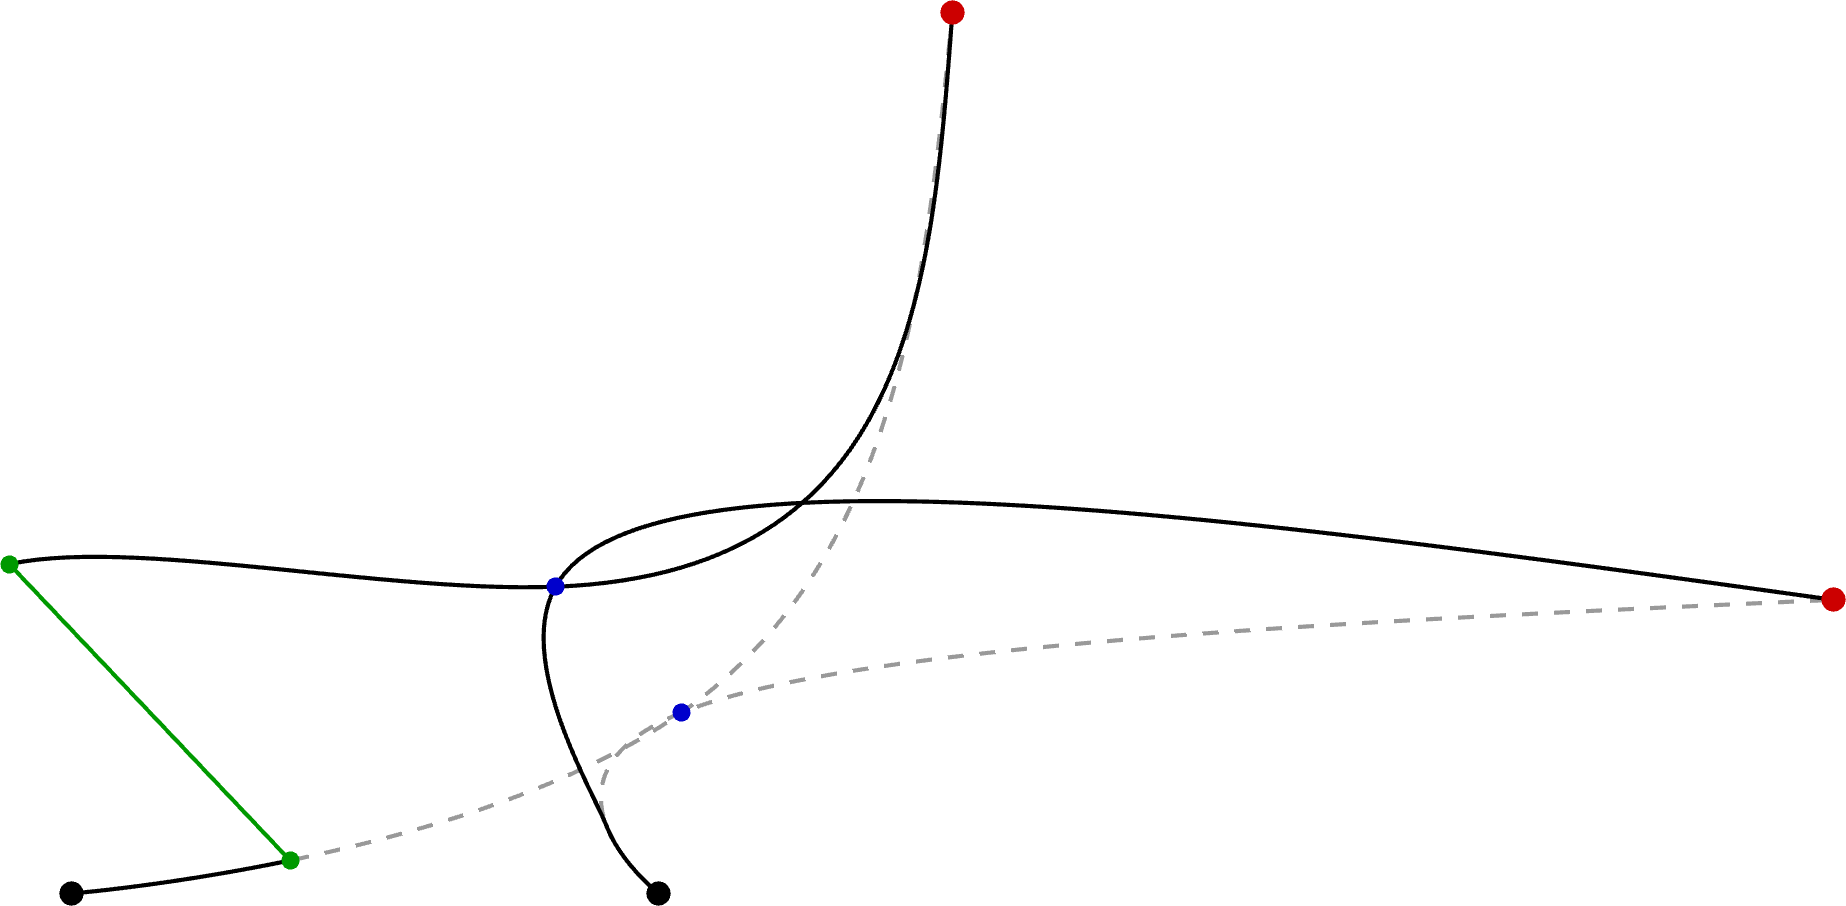
\includegraphics[width=.6\textwidth]{images/LQT_recursive_LS_multiAgents01.png}
\caption{\footnotesize
Least squares formulation of recursive LQR to control multiple agents (as point mass systems), where the task of each agent is to reach a desired target at the end of the motion, and to meet the other agent in the middle of the motion (e.g., for a handover task, see main text for the alternative option of nonzero offdiagonal elements at different time steps). We then test the adaptation capability of the agents by simulating a perturbation at 1/4 of the movement. The original and adapted movements are depicted in dashed and solid lines, respectively. The initial positions are represented with black points, the targets are in red, the optimized meeting points are in blue, and the perturbation is in green.
}
\label{fig:LQT_recursive_LS_multiAgents}
\end{SCfigure}

Figure \ref{fig:LQT_recursive_LS_multiAgents} presents an example with the control of multiple agents, with a precision matrix involving nonzero offdiagonal elements. The corresponding example code presents two options: it either requests the two agents to meet in the middle of the motion (e.g., for a handover task), or it requests the two agents to find a location to reach at different time steps (e.g., to drop and pick-up an object), involving nonzero offdiagonal elements at different time steps.


%The formulation can be used in the context of control primitives by first transforming each element of a dictionary $\bm{K}^\ty{D}_{i,t}$ to $\bm{\tilde{K}}^\ty{D}_{i,t}$ iteratively by starting from $\bm{\tilde{K}}_1=\bm{K}_1$, $\bm{U}_1=\bm{I}$, and by computing recursively
%\begin{align}
%	\bm{U}_t &= (\bm{A}_{t-1} + \bm{B}_{t-1} \bm{K}_{t-1}) \bm{U}_{t-1},\\
%	\bm{\tilde{K}}_t &= \bm{K}_t \bm{U}_t.
%\end{align}

%We can then redefine the above problem formulation as
%\begin{multline}
%	\min_{\bm{w}} \bm{x}^{\!\trsp} \bm{Q} \bm{x}
%	+
%	\big( \bm{\tilde{K}}^\ty{D} (\bm{w}\otimes\bm{I}) \bm{x}_1 \big)^{\!\trsp} \,\bm{R}\, \bm{\tilde{K}}^\ty{D} (\bm{w}\otimes\bm{I}) \bm{x}_1,\\
%	\text{s.t.}\;\;
%	\bm{x} = \big( \bm{S}_{\bm{x}}+\bm{S}_{\bm{u}} \bm{\tilde{K}}^\ty{D} (\bm{w}\otimes\bm{I}) \big) \bm{x}_1,
%\end{multline}
%where $\bm{w}$ is a vector of superposition weights and $\otimes$ is the Kronecker operator. The above problem can be solved in a similar way by noting that $\frac{\partial(\bm{w}\otimes\bm{I})}{\partial\bm{w}}=\bm{1}\otimes\bm{I}$. %Matrix cookbook (39) in Section 2

%In the LQT case, the elements of the dictionary $\bm{K}^\ty{D}_{i,t}$ can be formulated as both feedforward and feedback controllers.


%%%%%%%%%%%%%%%%%%%%%%%%%%%%%%%%%%%%%%%%%%%%%%%%%%%%%%%%%%%%%%%%%%%%%%%%%%%%%%%%%
\subsection{Dynamical movement primitives (DMP) reformulated as LQT with control primitives}\label{sec:DMPLQT}
\begin{flushright}
\filename{LQT\_CP\_DMP.*}
\end{flushright}

\begin{figure}
\centering
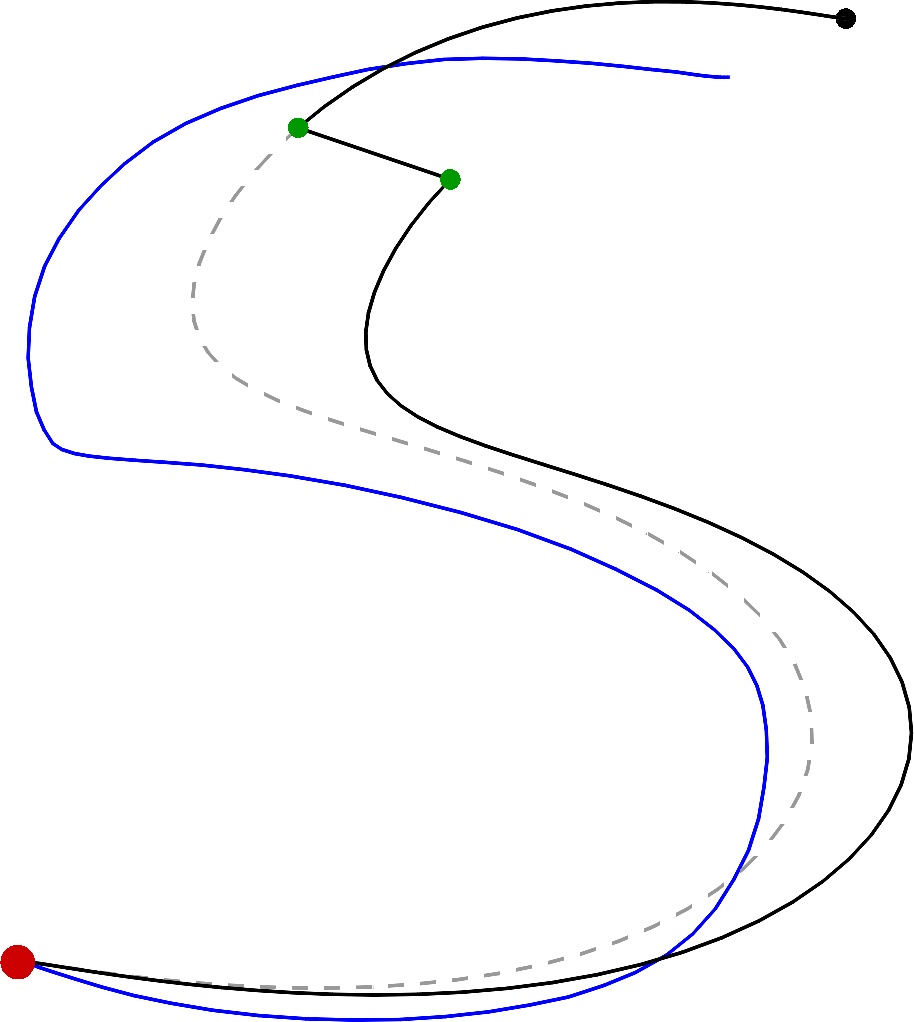
\includegraphics[width=.35\textwidth]{images/LQT_CP_DMP01.png}\hspace{6mm}
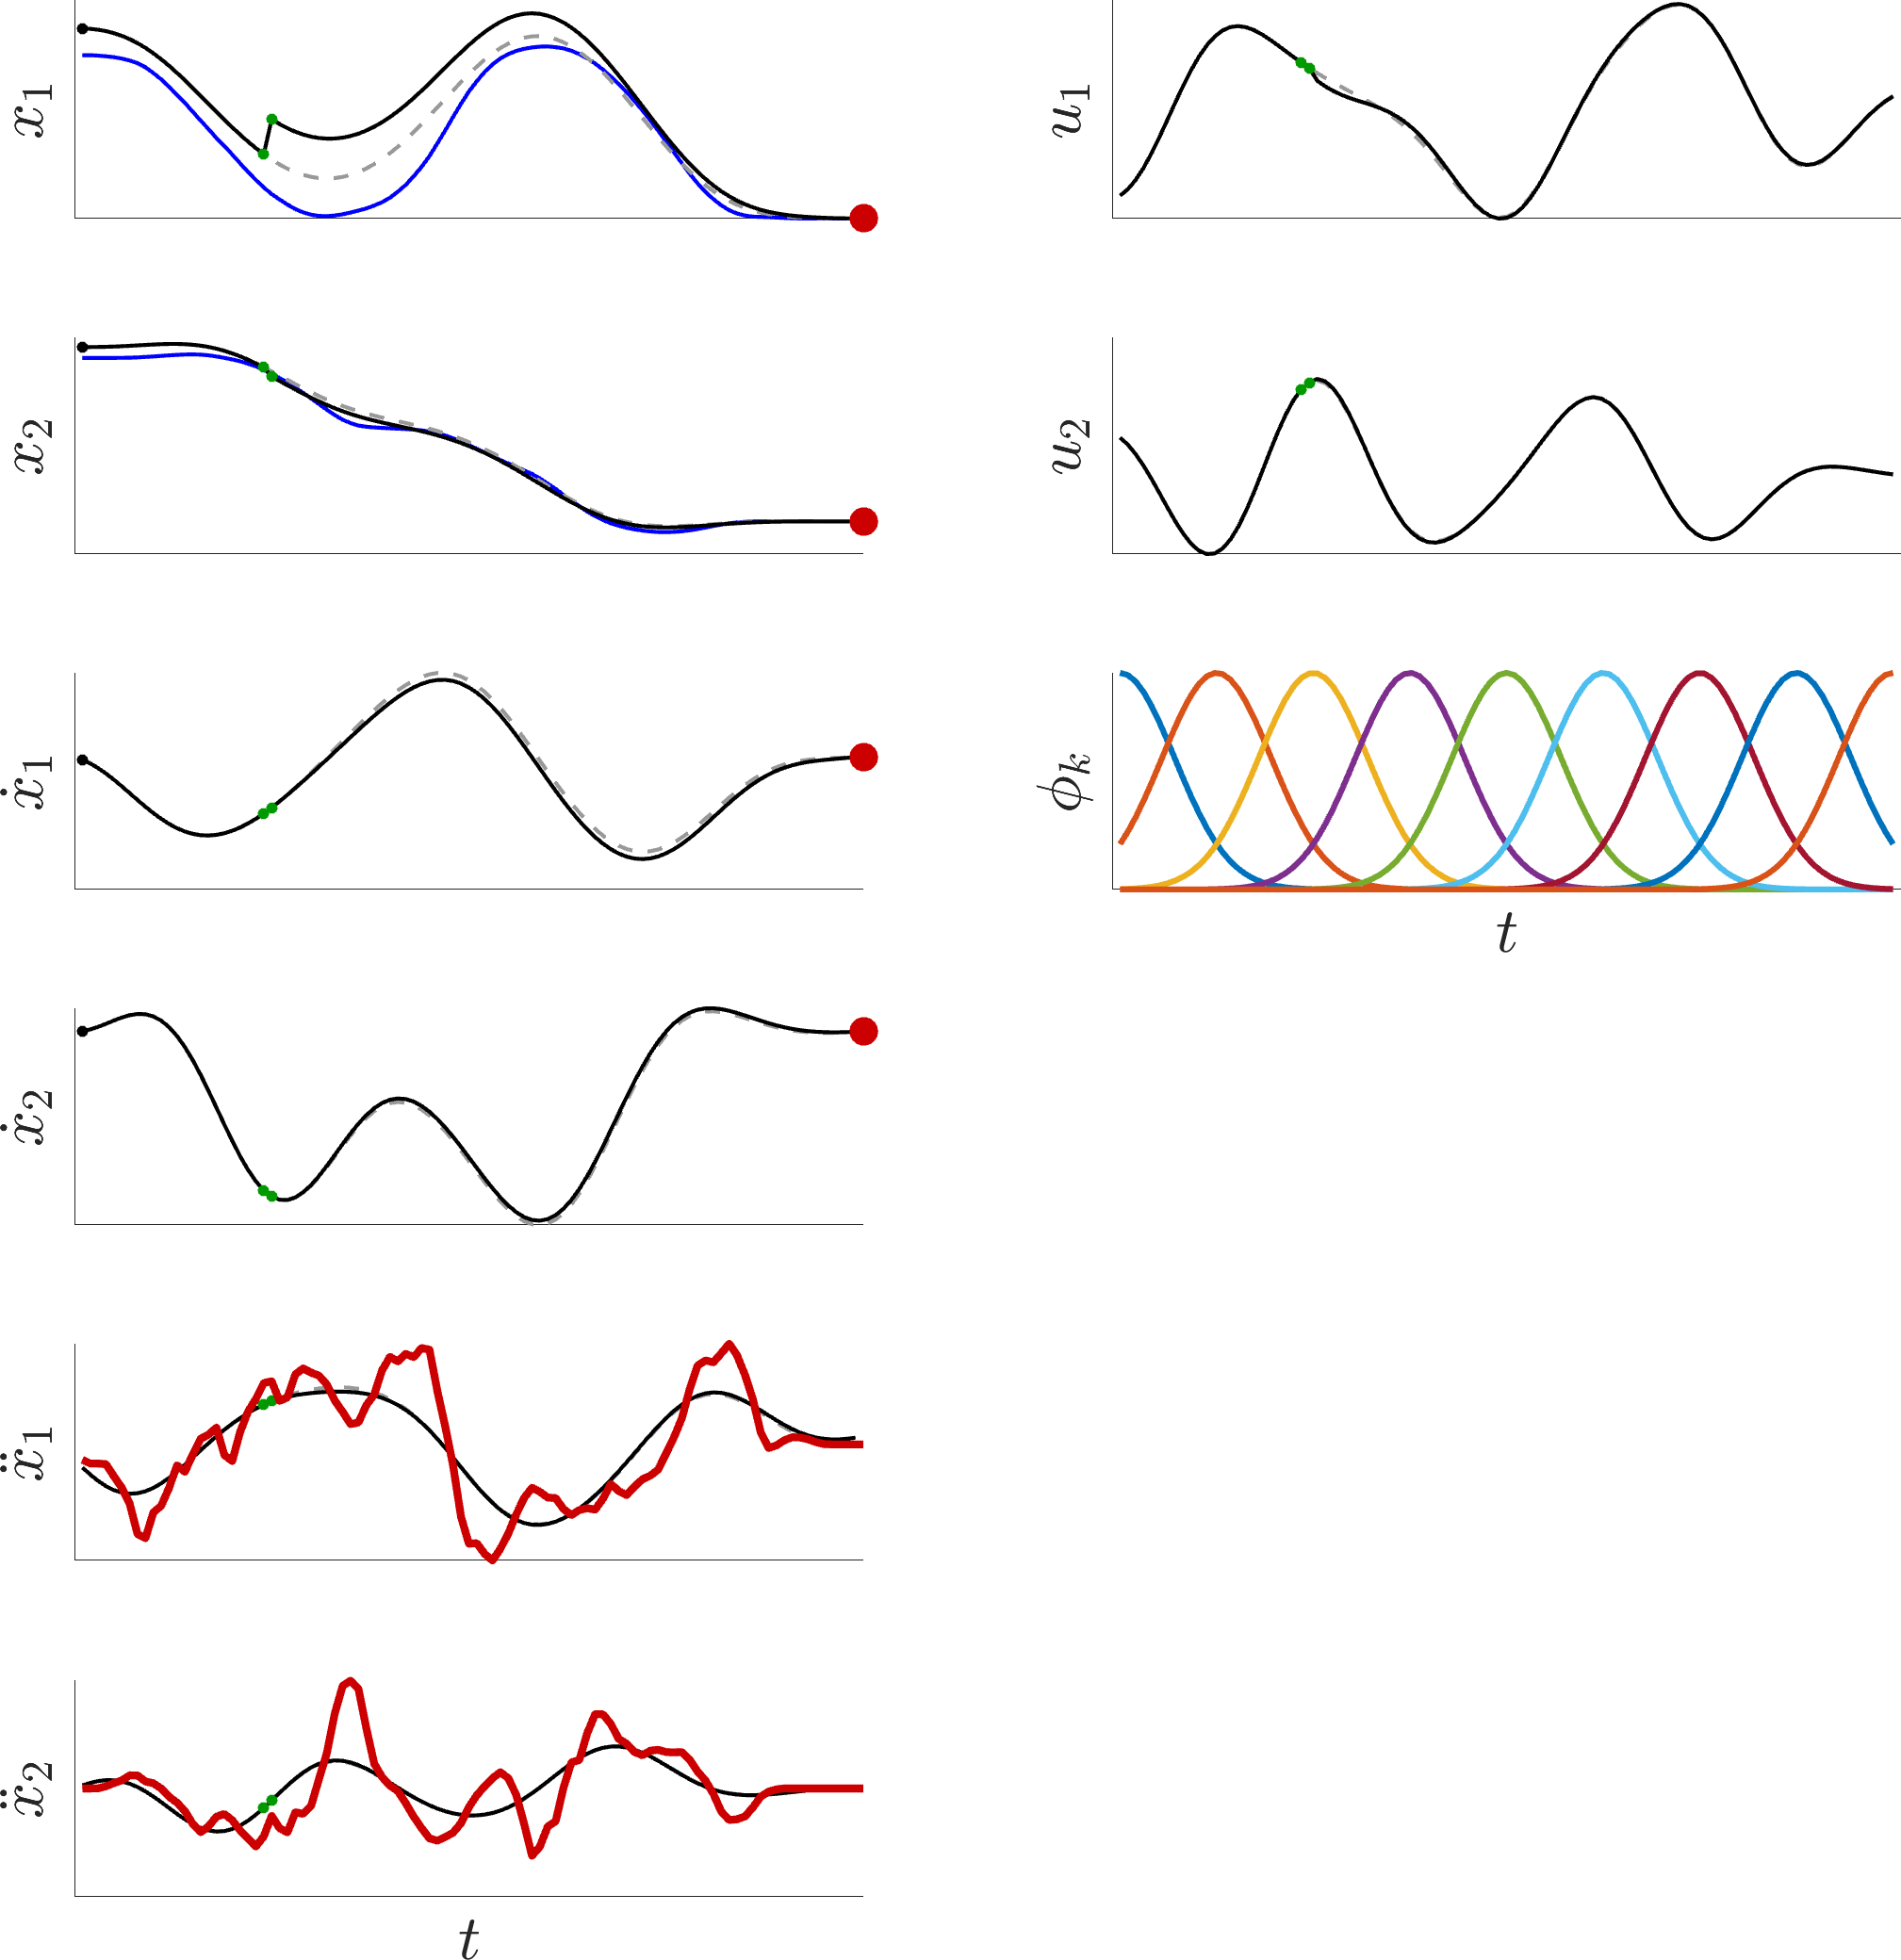
\includegraphics[width=.4\textwidth]{images/LQT_CP_DMP02.png}
\caption{\footnotesize
Linear quadratic tracking (LQT) with control primitives applied to a trajectory tracking task, with a formulation similar to dynamical movement primitives (DMP).
\emph{Left:} The observed ``S'' shape (in blue) is reproduced by starting from a different initial position (black point), with a perturbation simulated at 1/4 of the movement (green points) to show the capability of the approach to recover from perturbations. The trajectory in dashed line shows the result without perturbation and trajectory in solid line shows the result with perturbation.
\emph{Right:} The corresponding LQT problem formulation consists of requesting an end-point to be reached (red points) and an acceleration profile to be tracked (red lines), where the control commands $\bm{u}$ are represented as a superposition of radial basis functions $\bm{\phi}_k$.
}
\label{fig:LQT_CP_DMP}
\end{figure}

The dynamical movement primitives (DMP) \cite{Ijspeert13} approach proposes to reproduce an observed movement by crafting a controller composed of two parts: a closed-loop spring-damper system reaching the final point of the observed movement, and an open-loop system reproducing the acceleration profile of the observed movement. These two controllers are weighted so that the spring-damper system part is progressively increased until it becomes the only active controller. In DMP, the acceleration profile (also called forcing terms) is encoded with radial basis functions \cite{Broomhead88}, and the spring-damper system parameters are defined heuristically, usually as a critically damped system.

Linear quadratic tracking (LQT) with control primitives can be used in a similar fashion as in DMP, by requesting a target to be reached at the end of the movement and by requesting the observed acceleration profile to be tracked, while encoding the control commands as radial basis functions. The controller can be estimated either as the open-loop control commands \eqref{eq:uLQT}, or as the closed-loop controller \eqref{eq:uLQTrecursive}. 

In the latter case, the matrix $\bm{F}$ in \eqref{eq:LQR_LS_F} is estimated by using control primitives and an augmented state space formulation, namely
\begin{equation*}
	\bm{\hat{W}} = {\big(\bm{\Psi}^{\!\trsp} \bm{S}_{\bm{u}}^\trsp \bm{\tilde{Q}} \bm{S}_{\bm{u}} \bm{\Psi} + 
	\bm{\Psi}^{\!\trsp} \bm{R} \bm{\Psi}\big)}^{-1} \bm{\Psi}^{\!\trsp} \bm{S}_{\bm{u}}^\trsp \bm{\tilde{Q}} \bm{S}_{\bm{x}}, \quad
	\bm{F} = \bm{\Psi}\bm{\hat{W}},
	%\label{eq:LQR_LS_CP_F}
\end{equation*}
which is used to compute feedback gains $\bm{\tilde{K}}_t$ on the augmented state with \eqref{eq:K_from_F}.

The resulting controller $\bm{\hat{u}}_t = -\bm{\tilde{K}}_t \bm{\tilde{x}}_t$ tracks the acceleration profile while smoothly reaching the desired goal at the end of the movement, with a smooth transition between the two. The main difference with DMP is that the smooth transition between the two behaviors is directly optimized by the system, and the parameters of the feedback controller are automatically optimized (in DMP, stiffness and damping ratio). 

Figure \ref{fig:LQT_CP_DMP} presents an example of reproducing an ``S'' trajectory with simulation perturbations.

In addition, the LQT formulation allows the resulting controller to be formalized in the form of a cost function, which allows the approach to be combined more fluently with other optimal control strategies. Notably, the approach can be extended to multiple viapoints without any modification. It allows multiple demonstrations of a movement to be used to estimate a feedback controller that will exploit the (co)variations in the demonstrations to provide a minimal intervention control strategy that will selectively reject perturbations based on the impact they can have on the task to achieve. This is effectively attained by automatically regulating the gains in accordance to the variations in the demonstrations, with low gains in parts of the movement allowing variations, and higher gains for parts of the movement that are invariant in the demonstrations. It is also important to highlight that the solution of the LQT problem formulated as in the above is analytical, corresponding to a simple least squares problem.

Moreover, the above problem formulation can be extended to iterative LQR, providing an opportunity to consider obstacle avoidance and constraints within the DMP formulation, as well as to describe costs in task space with a DMP acting in joint angle space. 

\newpage

%%%%%%%%%%%%%%%%%%%%%%%%%%%%%%%%%%%%%%%%%%%%%%%%%%%%%%%%%%%%%%%%%%%%%%%%%%%%%%%%%
\section{iLQR optimization}

Optimal control problems are defined by a cost function $\sum_{t=1}^T c(\bm{x}_t,\bm{u}_t)$ to minimize and a dynamical system $\bm{x}_{t+1} = \bm{d}(\bm{x}_t,\bm{u}_t)$ describing the evolution of a state $\bm{x}_t$ driven by control commands $\bm{u}_t$ during a time window of length $T$.

Iterative LQR (iLQR) \cite{Li04} solves such constrained nonlinear models by carrying out Taylor expansions on the cost and on the dynamical system so that a solution can be found iteratively by solving a LQR problem at each iteration, similarly to differential dynamic programming approaches \cite{Mayne66,Rosenbrock72}.

iLQR employs a first order Taylor expansion of the dynamical system $\bm{x}_{t+1} = \bm{d}(\bm{x}_t,\bm{u}_t)$ around the point $(\bm{\hat{x}}_t, \bm{\hat{u}}_t)$, namely
\begin{align}
	\bm{x}_{t+1} &\approx \bm{d}(\bm{\hat{x}}_t,\bm{\hat{u}}_t) + \frac{\partial\bm{d}}{\partial\bm{x}_t} (\bm{x}_t-\bm{\hat{x}}_t) + \frac{\partial\bm{d}}{\partial\bm{u}_t} (\bm{u}_t-\bm{\hat{u}}_t) \nonumber\\
	\iff \Delta\bm{x}_{t+1} &\approx \bm{A}_t \Delta\bm{x}_t + \bm{B}_t \Delta\bm{u}_t,
	\label{eq:DS}
\end{align}
with residual vectors 
\begin{equation*}
	\Delta\bm{x}_t \!=\! \bm{x}_t \!-\! \bm{\hat{x}}_t, \quad
	\Delta\bm{u}_t \!=\! \bm{u}_t \!-\! \bm{\hat{u}}_t, 
\end{equation*}
and Jacobian matrices 
\begin{equation*}
\bm{A}_t = \frac{\partial\bm{d}}{\partial\bm{x}_t}\Big|_{\bm{\hat{x}}_t,\bm{\hat{u}}_t}, \quad 
\bm{B}_t = \frac{\partial\bm{d}}{\partial\bm{u}_t}\Big|_{\bm{\hat{x}}_t,\bm{\hat{u}}_t}.
\end{equation*}

The cost function $c(\bm{x}_t,\bm{u}_t)$ for time step $t$ can similarly be approximated by a second order Taylor expansion around the point $(\bm{\hat{x}}_t, \bm{\hat{u}}_t)$, namely
\begin{equation}
\begin{aligned}
	c(\bm{x}_t,\bm{u}_t) &\approx c(\bm{\hat{x}}_t,\bm{\hat{u}}_t) + \Delta\bm{x}_t^\trsp \frac{\partial c}{\partial\bm{x}_t} + 
	\Delta\bm{u}_t^\trsp \frac{\partial c}{\partial\bm{u}_t} +
	\frac{1}{2}\Delta\bm{x}_t^\trsp \frac{\partial^2c}{\partial\bm{x}_t^2} \Delta\bm{x}_t + 
	\Delta\bm{x}_t^\trsp \frac{\partial^2c}{\partial\bm{x}_t\bm{u}_t} \Delta\bm{u}_t +
	\frac{1}{2}\Delta\bm{u}_t^\trsp \frac{\partial^2c}{\partial\bm{u}_t^2} \Delta\bm{u}_t,
	\\
	\iff c(\bm{x}_t,\bm{u}_t) &\approx c(\bm{\hat{x}}_t,\bm{\hat{u}}_t) + 
	\frac{1}{2}
	\begin{bmatrix}
	1 \\ \Delta\bm{x}_t \\ \Delta\bm{u}_t
	\end{bmatrix}^{\!\trsp}
	\begin{bmatrix}
	0 & \bm{g}_{\bm{x},t}^\trsp & \bm{g}_{\bm{u},t}^\trsp \\
	\bm{g}_{\bm{x},t} & \bm{H}_{\bm{x}\bm{x},t} & \bm{H}_{\bm{u}\bm{x},t}^\trsp \\
	\bm{g}_{\bm{u},t} & \bm{H}_{\bm{u}\bm{x},t} & \bm{H}_{\bm{u}\bm{u},t} \\
	\end{bmatrix}
	\begin{bmatrix}
	1 \\ \Delta\bm{x}_t \\ \Delta\bm{u}_t
	\end{bmatrix},
\end{aligned}
\label{eq:dc}
\end{equation}
with gradients 
\begin{equation*}
	\bm{g}_{\bm{x},t}=\frac{\partial c}{\partial\bm{x}_t}\Big|_{\bm{\hat{x}}_t,\bm{\hat{u}}_t}, \quad  
	\bm{g}_{\bm{u},t}=\frac{\partial c}{\partial\bm{u}_t}\Big|_{\bm{\hat{x}}_t,\bm{\hat{u}}_t}, 
\end{equation*}
and Hessian matrices 
\begin{equation*}
	\bm{H}_{\bm{x}\bm{x},t}=\frac{\partial^2c}{\partial\bm{x}_t^2}\Big|_{\bm{\hat{x}}_t,\bm{\hat{u}}_t}, \quad  
	\bm{H}_{\bm{u}\bm{u},t}=\frac{\partial^2c}{\partial\bm{u}_t^2}\Big|_{\bm{\hat{x}}_t,\bm{\hat{u}}_t}, \quad
	\bm{H}_{\bm{u}\bm{x},t}=\frac{\partial^2c}{\partial\bm{u}_t\partial\bm{x}_t}\Big|_{\bm{\hat{x}}_t,\bm{\hat{u}}_t}.
\end{equation*}

%with gradients $\{\frac{\partial c}{\partial\bm{x}_t}, \frac{\partial c}{\partial\bm{u}_t}\}$, and Hessian matrices $\{\frac{\partial^2 c}{\partial\bm{x}_t^2}, \frac{\partial^2 c}{\partial\bm{x}_t\bm{u}_t}, \frac{\partial^2c}{\partial\bm{u}_t^2}\}$.


%%%%%%%%%%%%%%%%%%%%%%%%%%%%%%%%%%%%%%%%%%%%%%%%%%%%%%%%%%%%%%%%%%%%%%%%%%%%%%%%%
\subsection{Batch formulation of iLQR}\label{sec:iLQRbatch}
\begin{flushright}
\filename{iLQR\_manipulator.*}
\end{flushright}

A solution in batch form can be computed by minimizing over $\bm{u}\!=\!{\begin{bmatrix}\bm{u}_1^\trsp, \bm{u}_2^\trsp, \ldots, \bm{u}_{T-1}^\trsp \end{bmatrix}}^\trsp$, yielding a series of open loop control commands $\bm{u}_t$, corresponding to a Gauss--Newton iteration scheme, see Section \ref{sec:GaussNewton}. 

At a trajectory level, we denote $\bm{x}\!=\!{\begin{bmatrix}\bm{x}_1^\trsp, \bm{x}_2^\trsp, \ldots, \bm{x}_T^\trsp \end{bmatrix}}^\trsp$ %\!\in\!\mathbb{R}^{DCT}
the evolution of the state and $\bm{u}\!=\!{\begin{bmatrix}\bm{u}_1^\trsp, \bm{u}_2^\trsp, \ldots, \bm{u}_{T-1}^\trsp \end{bmatrix}}^\trsp$ %\!\in\!\mathbb{R}^{d(T-1)} 
the evolution of the control commands. 
The evolution of the state in \eqref{eq:DS} becomes $\Delta\bm{x} = \bm{S}_{\bm{u}} \Delta\bm{u}$, see Appendix \ref{app:Su} for details.\footnote{Note that $\bm{S}_{\bm{x}} \Delta\bm{x}_1\!=\!\bm{0}$ because $\Delta\bm{x}_1\!=\!\bm{0}$ (as we want our motion to start from $\bm{x}_1$).}

The minimization problem can then be rewritten in batch form as 
\begin{equation}
	\min_{\Delta\bm{u}} \Delta c(\Delta\bm{x},\Delta\bm{u}), \quad\text{s.t.}\quad \Delta\bm{x} = \bm{S}_{\bm{u}} \Delta\bm{u}, 
	\quad\text{where}\quad
	\Delta c(\Delta\bm{x},\Delta\bm{u}) = 
	\frac{1}{2}
	\begin{bmatrix}
	1 \\ \Delta\bm{x} \\ \Delta\bm{u}
	\end{bmatrix}^{\!\trsp}
	\begin{bmatrix}
	0 & \bm{g}_{\bm{x}}^\trsp & \bm{g}_{\bm{u}}^\trsp \\
	\bm{g}_{\bm{x}} & \bm{H}_{\bm{x}\bm{x}} & \bm{H}_{\bm{u}\bm{x}}^\trsp \\
	\bm{g}_{\bm{u}} & \bm{H}_{\bm{u}\bm{x}} & \bm{H}_{\bm{u}\bm{u}} \\
	\end{bmatrix}
	\begin{bmatrix}
	1 \\ \Delta\bm{x} \\ \Delta\bm{u}
	\end{bmatrix}.
	%\Delta\bm{x}^\trsp \bm{g}_{\bm{x}} + \Delta\bm{u}^\trsp \bm{g}_{\bm{u}} +\\
	%\frac{1}{2} \Delta\bm{x}^\trsp \bm{H}_{\bm{x}\bm{x}} \Delta\bm{x} + 
	%\Delta\bm{x}^\trsp \bm{H}_{\bm{x}\bm{u}} \Delta\bm{u} +
	%\frac{1}{2} \Delta\bm{u}^\trsp \bm{H}_{\bm{u}\bm{u}} \Delta\bm{u}.
	\label{eq:dc_batch}
\end{equation} 

By inserting the constraint into the cost, we obtain the optimization problem
\begin{equation}
	\min_{\Delta\bm{u}} \quad
	\Delta\bm{u}^\trsp \bm{S}_{\bm{u}}^\trsp \bm{g}_{\bm{x}} + \Delta\bm{u}^\trsp \bm{g}_{\bm{u}} +
	\frac{1}{2} \Delta\bm{u}^\trsp \bm{S}_{\bm{u}}^\trsp \bm{H}_{\bm{x}\bm{x}} \bm{S}_{\bm{u}} \Delta\bm{u} +
	\Delta\bm{u}^\trsp \bm{S}_{\bm{u}}^\trsp \bm{H}_{\bm{u}\bm{x}}^\trsp \Delta\bm{u} +
	\frac{1}{2} \Delta\bm{u}^\trsp \bm{H}_{\bm{u}\bm{u}} \Delta\bm{u},
	\label{eq:minu}
\end{equation}
which can be solved analytically by differentiating with respect to $\Delta\bm{u}$ and equating to zero, namely,
\begin{equation}
	\bm{S}_{\bm{u}}^\trsp \bm{g}_{\bm{x}} + \bm{g}_{\bm{u}} +\\
	\bm{S}_{\bm{u}}^\trsp \bm{H}_{\bm{x}\bm{x}} \bm{S}_{\bm{u}} \Delta\bm{u} + 
	2 \bm{S}_{\bm{u}}^\trsp \bm{H}_{\bm{u}\bm{x}}^\trsp \Delta\bm{u} +
	\bm{H}_{\bm{u}\bm{u}} \Delta\bm{u} = 0,
\end{equation}
providing the least squares solution
\begin{equation}
	\Delta\bm{\hat{u}} =
	{\left( \bm{S}_{\bm{u}}^\trsp \bm{H}_{\bm{x}\bm{x}} \bm{S}_{\bm{u}} + 2 \bm{S}_{\bm{u}}^\trsp \bm{H}_{\bm{u}\bm{x}}^\trsp + \bm{H}_{\bm{u}\bm{u}} \right)}^{-1}
	\left(-\bm{S}_{\bm{u}}^\trsp \bm{g}_{\bm{x}} - \bm{g}_{\bm{u}}\right),
	\label{eq:du_general}
\end{equation}
which can be used to update the control commands estimate at each iteration step of the iLQR algorithm.

\begin{figure}
\centering
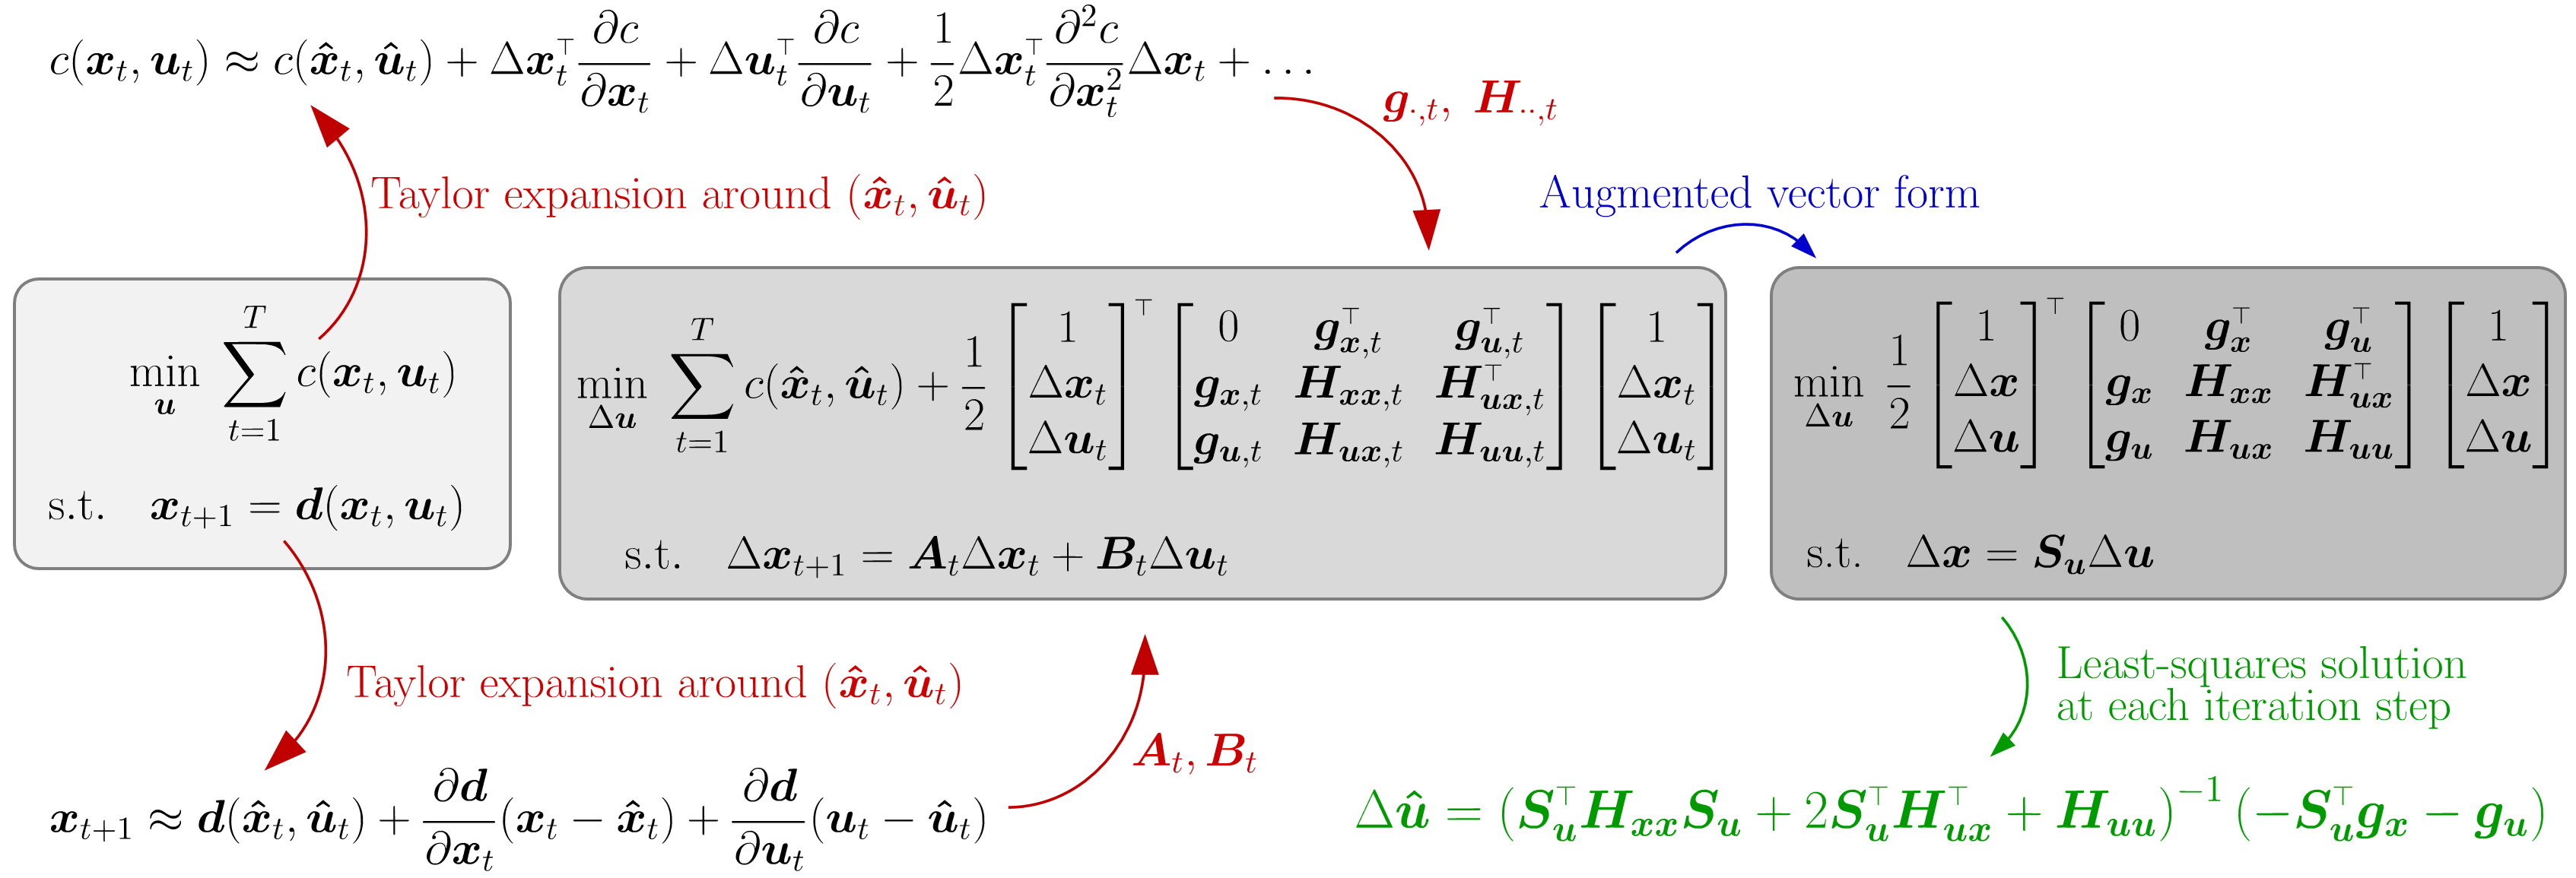
\includegraphics[width=.9\columnwidth]{images/iLQR-eqs-overview01.png}
\caption{\footnotesize
Summary of the iLQR optimization procedure in batch form.
}
\label{fig:iLQR_summary}
\end{figure}

The complete iLQR procedure is described in Algorithm \ref{alg:iLQRbatch} (including backtracking line search). Figure \ref{fig:iLQR_summary} also presents an illustrative summary of the iLQR optimization procedure in batch form.



%%%%%%%%%%%%%%%%%%%%%%%%%%%%%%%%%%%%%%%%%%%%%%%%%%%%%%%%%%%%%%%%%%%%%%%%%%%%%%%%%
\subsection{Recursive formulation of iLQR}\label{sec:iLQRrecursive}
\begin{flushright}
\filename{iLQR\_manipulator\_recursive.*}
\end{flushright}
%See also https://homes.cs.washington.edu/~todorov/papers/TassaIROS12.pdf

A solution can alternatively be computed in a recursive form to provide a controller with feedback gains. Section \ref{sec:LQRrecursive} presented the dynamic programming principle in the context of linear quadratic regulation problems, which allowed us to reduce the minimization over an entire sequence of control commands to a sequence of minimization problems over control commands at a single time step, by proceeding backwards in time. In this section, the approach is extended to iLQR. 

Similarly to \eqref{eq:qtLQR}, we have here
\begin{align}
	\hat{v}_t(\Delta\bm{x}_t) &= \min_{\Delta\bm{u}_t} \, \underbrace{c_t(\Delta\bm{x}_t,\Delta\bm{u}_t) + \hat{v}_{t+1}(\Delta\bm{x}_{t+1})}_{q_t(\Delta\bm{x}_t,\Delta\bm{u}_t)},
	\label{eq:qtiLQR}
\end{align}

Similarly to LQR, by starting from the last time step $T$, $\hat{v}_T(\Delta\bm{x}_T)$ is independent of the control commands. By relabeling $\bm{g}_{\bm{x},T}$ and $\bm{H}_{\bm{x}\bm{x},T}$ as $\bm{v}_{\bm{x},T}$ and $\bm{V}_{\bm{x}\bm{x},T}$, we can show that $\hat{v}_{T-1}$ has the same quadratic form as $\hat{v}_{T}$, enabling the backward recursive computation of $\hat{v}_{t}$ from $t=T-1$ to $t=1$.

This dynamic programming recursion takes the form 
\begin{equation}
	\hat{v}_{t+1} =
	\begin{bmatrix}
	1 \\ \Delta\bm{x}_{t+1}
	\end{bmatrix}^{\!\trsp}
	\begin{bmatrix}
	0 & \bm{v}_{\bm{x},{t+1}}^\trsp \\
	\bm{v}_{\bm{x},{t+1}} & \bm{V}_{\bm{x}\bm{x},{t+1}} 
	\end{bmatrix}
	\begin{bmatrix}
	1 \\ \Delta\bm{x}_{t+1}
	\end{bmatrix},
	\label{eq:vhatTiLQR}
\end{equation}
and we then have with \eqref{eq:qtiLQR} that
\begin{equation}
	\hat{v}_{t} = \min_{\Delta\bm{u}_{t}} 
	\begin{bmatrix}
	1 \\ \Delta\bm{x}_{t} \\ \Delta\bm{u}_{t}
	\end{bmatrix}^{\!\trsp}
	\begin{bmatrix}
	0 & \bm{g}_{\bm{x},{t}}^\trsp & \bm{g}_{\bm{u},{t}}^\trsp \\
	\bm{g}_{\bm{x},{t}} & \bm{H}_{\bm{x}\bm{x},{t}} & \bm{H}_{\bm{u}\bm{x},{t}}^\trsp \\
	\bm{g}_{\bm{u},{t}} & \bm{H}_{\bm{u}\bm{x},{t}} & \bm{H}_{\bm{u}\bm{u},{t}} \\
	\end{bmatrix}
	\begin{bmatrix}
	1 \\ \Delta\bm{x}_{t} \\ \Delta\bm{u}_{t}
	\end{bmatrix}
	+ 
	\begin{bmatrix}
	1 \\ \Delta\bm{x}_{t+1}
	\end{bmatrix}^{\!\trsp}
	\begin{bmatrix}
	0 & \bm{v}_{\bm{x},{t+1}}^\trsp \\
	\bm{v}_{\bm{x},{t+1}} & \bm{V}_{\bm{x}\bm{x},{t+1}} 
	\end{bmatrix}
	\begin{bmatrix}
	1 \\ \Delta\bm{x}_{t+1}
	\end{bmatrix}.
	\label{eq:ct0iLQR}
\end{equation}

By substituting $\Delta\bm{x}_{t+1} = \bm{A}_{t} \Delta\bm{x}_{t} + \bm{B}_{t} \Delta\bm{u}_{t}$ into \eqref{eq:ct0iLQR}, $\hat{v}_{t}$ can be rewritten as
\begin{equation}
	\hat{v}_{t} = \min_{\Delta\bm{u}_{t}}
	\begin{bmatrix}
	1 \\ \Delta\bm{x}_t \\ \Delta\bm{u}_t
	\end{bmatrix}^{\!\!\trsp} \!\!
	\begin{bmatrix}
	0 & \bm{q}_{\bm{x},t}^\trsp & \bm{q}_{\bm{u},t}^\trsp \\
	\bm{q}_{\bm{x},t} & \bm{Q}_{\bm{x}\bm{x},t} & \bm{Q}_{\bm{u}\bm{x},t}^\trsp \\
	\bm{q}_{\bm{u},t} & \bm{Q}_{\bm{u}\bm{x},t} & \bm{Q}_{\bm{u}\bm{u},t} \\
	\end{bmatrix} \!\!
	\begin{bmatrix}
	1 \\ \Delta\bm{x}_t \\ \Delta\bm{u}_t
	\end{bmatrix},
	\quad\text{where}\quad 
	\left\{
	\begin{aligned}
		\bm{q}_{\bm{x},t} &= \bm{g}_{\bm{x},t} + \bm{A}_t^\trsp \bm{v}_{\bm{x},t+1}, \\
		\bm{q}_{\bm{u},t} &= \bm{g}_{\bm{u},t} + \bm{B}_t^\trsp \, \bm{v}_{\bm{x},t+1}, \\
		\bm{Q}_{\bm{x}\bm{x},t} &\approx \bm{H}_{\bm{x}\bm{x},t} + \bm{A}_t^\trsp \, \bm{V}_{\bm{x}\bm{x},t+1} \, \bm{A}_t, \\
		\bm{Q}_{\bm{u}\bm{u},t} &\approx \bm{H}_{\bm{u}\bm{u},t} + \bm{B}_t^\trsp \, \bm{V}_{\bm{x}\bm{x},t+1} \, \bm{B}_t, \\
		\bm{Q}_{\bm{u}\bm{x},t} &\approx \bm{H}_{\bm{u}\bm{x},t} + \bm{B}_t^\trsp \, \bm{V}_{\bm{x}\bm{x},t+1} \, \bm{A}_t, 
	\end{aligned}
	\right.
	\label{eq:qt} %{eq:ct1iLQR}
\end{equation}
with gradients 
\begin{equation*}
	\bm{g}_{\bm{x},t} = \frac{\partial c}{\partial\bm{x}_t}\Big|_{\bm{\hat{x}}_t,\bm{\hat{u}}_t}, \quad
	\bm{g}_{\bm{u},t} = \frac{\partial c}{\partial\bm{u}_t}\Big|_{\bm{\hat{x}}_t,\bm{\hat{u}}_t}, \quad
	\bm{v}_{\bm{x},t} = \frac{\partial \hat{v}}{\partial\bm{x}_t}\Big|_{\bm{\hat{x}}_t,\bm{\hat{u}}_t}, \quad 
	\bm{q}_{\bm{x},t} = \frac{\partial q}{\partial\bm{x}_t}\Big|_{\bm{\hat{x}}_t,\bm{\hat{u}}_t}, \quad 
	\bm{q}_{\bm{u},t} = \frac{\partial q}{\partial\bm{u}_t}\Big|_{\bm{\hat{x}}_t,\bm{\hat{u}}_t},
\end{equation*}
Jacobian matrices 
\begin{equation*}
	\bm{A}_t = \frac{\partial\bm{d}}{\partial\bm{x}_t}\Big|_{\bm{\hat{x}}_t,\bm{\hat{u}}_t}, \quad
	\bm{B}_t = \frac{\partial\bm{d}}{\partial\bm{u}_t}\Big|_{\bm{\hat{x}}_t,\bm{\hat{u}}_t},
\end{equation*}
and Hessian matrices 
\begin{equation*}
	\bm{H}_{\bm{x}\bm{x},t} \!=\! \frac{\partial^2 c}{\partial\bm{x}_t^2}\Big|_{\bm{\hat{x}}_t,\bm{\hat{u}}_t}, \quad 
	\bm{H}_{\bm{u}\bm{u},t} \!=\! \frac{\partial^2 c}{\partial\bm{u}_t^2}\Big|_{\bm{\hat{x}}_t,\bm{\hat{u}}_t}, \quad 
	\bm{H}_{\bm{u}\bm{x},t} \!=\! \frac{\partial^2 c}{\partial\bm{u}_t\partial\bm{x}_t}\Big|_{\bm{\hat{x}}_t,\bm{\hat{u}}_t}, \quad 
	\bm{V}_{\bm{x}\bm{x},t} \!=\! \frac{\partial^2 \hat{v}}{\partial\bm{x}_t^2}\Big|_{\bm{\hat{x}}_t,\bm{\hat{u}}_t},
\end{equation*}
\begin{equation*}	
	\bm{Q}_{\bm{x}\bm{x},t} = \frac{\partial^2 q}{\partial\bm{x}_t^2}\Big|_{\bm{\hat{x}}_t,\bm{\hat{u}}_t}, \quad
	\bm{Q}_{\bm{u}\bm{u},t} = \frac{\partial^2 q}{\partial\bm{u}_t^2}\Big|_{\bm{\hat{x}}_t,\bm{\hat{u}}_t}, \quad 
	\bm{Q}_{\bm{u}\bm{x},t} = \frac{\partial^2 q}{\partial\bm{u}_t\partial\bm{x}_t}\Big|_{\bm{\hat{x}}_t,\bm{\hat{u}}_t}.
\end{equation*}
%Bold lower case letter refer to gradient vectors and bold upper case letter refer to Hessian matrices.
%, with the alphabet letter corresponding to the function they refer to.

Minimizing \eqref{eq:qt} w.r.t.~$\Delta\bm{u}_t$ can be achieved by differentiating the equation and equating to zero, yielding the controller
\begin{equation}
	\Delta\bm{\hat{u}}_t = \bm{k}_t + \bm{K}_t \, \Delta\bm{x}_t,
	\;\text{with}\quad
	\left\{
	\begin{aligned}
	\bm{k}_t &= - \bm{Q}_{\bm{u}\bm{u},t}^{-1} \, \bm{q}_{\bm{u},t}, \\
	\bm{K}_t &= - \bm{Q}_{\bm{u}\bm{u},t}^{-1} \, \bm{Q}_{\bm{u}\bm{x},t}, 
	\end{aligned}
	\right.
	\label{eq:duhat}
\end{equation}
where $\bm{k}_t$ is a feedforward command and $\bm{K}_t$ is a feedback gain matrix.

By inserting \eqref{eq:duhat} into \eqref{eq:qt}, we get the recursive updates
\begin{equation}
\begin{aligned}
	\bm{v}_{\bm{x},t} &= \bm{q}_{\bm{x},t} - \bm{Q}_{\bm{u}\bm{x},t}^\trsp \, \bm{Q}_{\bm{u}\bm{u},t}^{-1} \, \bm{q}_{\bm{u},t}, \\
	\bm{V}_{\bm{x}\bm{x},t} &= \bm{Q}_{\bm{x}\bm{x},t} - \bm{Q}_{\bm{u}\bm{x},t}^\trsp \, \bm{Q}_{\bm{u}\bm{u},t}^{-1} \, \bm{Q}_{\bm{u}\bm{x},t}.
\end{aligned}
\label{eq:vV} 
\end{equation}

In this recursive iLQR formulation, at each iteration step of the optimization algorithm, the nominal trajectories $(\bm{\hat{x}}_t, \bm{\hat{u}}_t)$ are refined, together with feedback matrices $\bm{K}_t$. Thus, at each iteration step of the optimization algorithm, a backward and forward recursion is performed to evaluate these vectors and matrices. There is thus two types of iterations: one for the optimization algorithm, and one for the dynamic programming recursion performed at each given iteration.

After convergence, by using \eqref{eq:duhat} and the nominal trajectories in the state and control spaces $(\bm{\hat{x}}_t, \bm{\hat{u}}_t)$, the resulting controller at each time step $t$ is
\begin{equation}
	\bm{u}_t = \bm{\hat{u}}_t + \bm{K}_t \, (\bm{\hat{x}}_t - \bm{x}_t),
	\label{eq:iLQRrecursiveController}
\end{equation}
where the evolution of the state is described by $\bm{x}_{t+1}=\bm{d}(\bm{x}_{t},\bm{u}_{t})$.

The complete iLQR procedure is described in Algorithm \ref{alg:iLQRrecursive} (including backtracking line search).

%As in Section \ref{sec:LQRrecursive}, we start from the minimization with respect to $\bm{u}_t$ of a cumulative partial cost function $v(\bm{x}_t,\bm{u}_t)$ as in \eqref{eq:cumulativeCost}. 

%With the dynamic programming principle, the minimization over a sequence of control commands is reduced to a sequence of minimization problems over a single control command. This is achieved by proceeding backwards in time with the same recursive form as in Section \ref{sec:LQRrecursive}.
%, by considering the cost
%\begin{equation}
%	q(\bm{x}_{t:T},\bm{u}_t) = c(\bm{x}_t,\bm{u}_t) + \hat{v}(\bm{x}_{t+1:T}).
%	\label{eq:iLRQct}
%\end{equation}

%Similarly to \eqref{eq:dc}, $v(\bm{x}_t,\bm{u}_t)$ can be approximated by a second order Taylor expansion around the point $(\bm{\hat{x}}_t, \bm{\hat{u}}_t)$, yielding 
%\begin{equation*}
%	\Delta q(\Delta\bm{x}_t,\Delta\bm{u}_t) \approx 
%	\begin{bmatrix}
%	1 \\ \Delta\bm{x}_t \\ \Delta\bm{u}_t
%	\end{bmatrix}^{\!\!\trsp} \!\!
%	\begin{bmatrix}
%	0 & \bm{q}_{\bm{x},t}^\trsp & \bm{q}_{\bm{u},t}^\trsp \\
%	\bm{q}_{\bm{x},t} & \bm{Q}_{\bm{x}\bm{x},t} & \bm{Q}_{\bm{u}\bm{x},t}^\trsp \\
%	\bm{q}_{\bm{u},t} & \bm{Q}_{\bm{u}\bm{x},t} & \bm{Q}_{\bm{u}\bm{u},t} \\
%	\end{bmatrix} \!\!
%	\begin{bmatrix}
%	1 \\ \Delta\bm{x}_t \\ \Delta\bm{u}_t
%	\end{bmatrix},
%\end{equation*}
%\begin{equation}
%\begin{aligned}
%	\text{where} \hspace{5mm} \bm{q}_{\bm{x},t} &= \bm{g}_{\bm{x},t} + \bm{A}_t^\trsp \bm{v}_{\bm{x},t+1}, \\
%	\bm{q}_{\bm{u},t} &= \bm{g}_{\bm{u},t} + \bm{B}_t^\trsp \, \bm{v}_{\bm{x},t+1}, \\
%	\bm{Q}_{\bm{x}\bm{x},t} &\approx \bm{H}_{\bm{x}\bm{x},t} + \bm{A}_t^\trsp \, \bm{V}_{\bm{x}\bm{x},t+1} \, \bm{A}_t, \\
%	\bm{Q}_{\bm{u}\bm{u},t} &\approx \bm{H}_{\bm{u}\bm{u},t} + \bm{B}_t^\trsp \, \bm{V}_{\bm{x}\bm{x},t+1} \, \bm{B}_t, \\
%	\bm{Q}_{\bm{u}\bm{x},t} &\approx \bm{H}_{\bm{u}\bm{x},t} + \bm{B}_t^\trsp \, \bm{V}_{\bm{x}\bm{x},t+1} \, \bm{A}_t, 
%\end{aligned}
%\label{eq:qt}
%\end{equation}

%%%%%%%%%%%%%%%%%%%%%%%%%%%%%%%%%%%%%%%%%%%%%%%%%%%%%%%%%%%%%%%%%%%%%%%%%%%%%%%%%
\subsection{Least squares formulation of recursive iLQR}\label{sec:iLQRLS}

First, note that \eqref{eq:duhat} can be rewritten as
\begin{equation}
	\Delta\bm{\hat{u}}_t = \bm{\tilde{K}}_t \, \begin{bmatrix} \Delta\bm{x}_t \\ 1 \end{bmatrix},
	\;\text{with}\quad
	\bm{\tilde{K}}_t = - \bm{Q}_{\bm{u}\bm{u},t}^{-1} \Big[ \bm{Q}_{\bm{u}\bm{x},t}, \; \bm{q}_{\bm{u},t} \Big]. 
\label{eq:duhat2}
\end{equation}

Also, \eqref{eq:minu} can be rewritten as
\begin{equation*}
	\min_{\Delta\bm{u}} \quad \underbrace{\frac{1}{2}
	\begin{bmatrix} \Delta\bm{u} \\ 1 \end{bmatrix}^\trsp
	\begin{bmatrix} \bm{C} & \bm{c} \\ \bm{c}^\trsp & 0 \end{bmatrix}
	\begin{bmatrix} \Delta\bm{u} \\ 1 \end{bmatrix}}_{\frac{1}{2} \Delta\bm{u}^\trsp \bm{C} \Delta\bm{u} + \Delta\bm{u}^\trsp \bm{c}},
	\quad\text{where}\quad
	\left\{
	\begin{aligned}
	\bm{c} &= \bm{S}_{\bm{u}}^\trsp \bm{g}_{\bm{x}} + \bm{g}_{\bm{u}}, \\
	\bm{C} &= \bm{S}_{\bm{u}}^\trsp \bm{H}_{\bm{x}\bm{x}} \bm{S}_{\bm{u}} 
	+ 2 \bm{S}_{\bm{u}}^\trsp \bm{H}_{\bm{u}\bm{x}}^\trsp
	+ \bm{H}_{\bm{u}\bm{u}}.
	\end{aligned}
	\right.
\end{equation*}

Similarly to Section \ref{sec:LQRLS}, we set 
\begin{equation}
	\Delta\bm{u} = -\bm{F} \begin{bmatrix} \Delta\bm{x}_1 \\ 1 \end{bmatrix} 
	= -\bm{F} \begin{bmatrix} \bm{0} \\ 1 \end{bmatrix}
	= -\bm{F} \Delta\bm{\tilde{x}}_1, 
\end{equation}
and redefine the optimization problem as
\begin{equation}
	\min_{\bm{F}} \quad \frac{1}{2} \Delta\bm{\tilde{x}}_1^\trsp \bm{F}^\trsp \bm{C} \bm{F} \Delta\bm{\tilde{x}}_1 
	- \Delta\bm{\tilde{x}}_1^\trsp \bm{F}^\trsp \bm{c}.
\end{equation}

By differentiating w.r.t.\ $\bm{F}$ and equating to zero, we get
\begin{equation}
	\bm{F} \Delta\bm{\tilde{x}}_1 = \bm{C}^{-1} \bm{c}.
\end{equation}

Similarly to Section \ref{sec:LQRLS}, we decompose $\bm{F}$ as block matrices $\bm{F}_t$ with $t\in\{1,\ldots,T-1\}$. $\bm{F}$ can then be used to iteratively reconstruct regulation gains $\bm{K}_t$, by starting from $\bm{K}_1=\bm{F}_1$, $\bm{P}_1=\bm{I}$, and by computing with forward recursion
\begin{equation}
	\bm{P}_t = \bm{P}_{t-1} {(\bm{A}_{t-1} - \bm{B}_{t-1} \bm{K}_{t-1})}^{-1}, \quad
	\bm{K}_t = \bm{F}_t \; \bm{P}_t,
\end{equation}
from $t=2$ to $t=T-1$.


%%%%%%%%%%%%%%%%%%%%%%%%%%%%%%%%%%%%%%%%%%%%%%%%%%%%%%%%%%%%%%%%%%%%%%%%%%%%%%%%%
\subsection{Updates by considering step sizes}
\begin{flushright}
\filename{iLQR\_manipulator.*}
\end{flushright}

\begin{algorithm}
\caption{Backtracking line search method with parameter $\alpha_{\min}$}
\label{alg:linesearch}
$\alpha \gets 1$ \\
\While{$c(\bm{\hat{u}}+\alpha\;\Delta\bm{\hat{u}}) > c(\bm{\hat{u}}) \;\textbf{and}\;\; \alpha > \alpha_{\min}$}{
	$\alpha \gets \frac{\alpha}{2}$
}
\end{algorithm}

\begin{algorithm}
\caption{Batch formulation of iLQR}
\label{alg:iLQRbatch}
Define cost $c(\cdot)$, dynamics $\bm{d}(\cdot)$, $\bm{x}_1$, $\alpha_{\min}$, $\Delta_{\min}$ \\
Initialize $\bm{\hat{u}}$ \\
\Repeat{$\|\Delta\bm{\hat{u}}\| < \Delta_{\min}$}{
	Compute $\bm{\hat{x}}$ using $\bm{\hat{u}}$, $\bm{d}(\cdot)$, and $\bm{x}_1$ \\
	Compute $\bm{A}_t, \bm{B}_t$ in \eqref{eq:DS} \\
	Compute $\bm{S}_{\bm{u}}$ with \eqref{eq:SxSu} \\ 
	Compute $\bm{g}_{\bm{\cdot}}$ and $\bm{H}_{\bm{\cdot}}$ in \eqref{eq:dc_batch}, using \eqref{eq:dc} \\
	Compute $\Delta\bm{\hat{u}}$ with \eqref{eq:du_general} \\
	Compute $\alpha$ with Algorithm \ref{alg:linesearch} \\
	Update $\bm{\hat{u}}$ with \eqref{eq:alpha} 
} 
\end{algorithm}

\begin{algorithm}
\caption{Recursive formulation of iLQR}
\label{alg:iLQRrecursive}
Define cost $c(\cdot)$, dynamics $\bm{d}(\cdot)$, $\bm{x}_1$, $\alpha_{\min}$, $\Delta_{\min}$ \\
Initialize all $\bm{\hat{u}}_t$ \\
\Repeat{$\|\Delta\bm{\hat{u}}\| < \Delta_{\min}$}{
	Compute $\bm{\hat{x}}$ using $\bm{\hat{u}}$, $\bm{d}(\cdot)$, and $\bm{x}_1$ \\
	\tcp{Evaluating derivatives} 
	Compute all $\bm{A}_t, \bm{B}_t$ in \eqref{eq:DS} \\
	Compute all $\bm{g}_{\bm{\cdot},t}$ and $\bm{H}_{\bm{\cdot},t}$ in \eqref{eq:dc} \\
	\tcp{Backward pass} 
	Set $\bm{v}_{\bm{x},T}=\bm{g}_{\bm{x},T}$ and $\bm{V}_{\bm{x}\bm{x},T}=\bm{H}_{\bm{x}\bm{x},T}$ \\
	\For{$t \gets T-1$ to $1$}{
		Compute $\bm{q}_{\bm{\cdot},t}$ and $\bm{Q}_{\bm{\cdot},t}$ with \eqref{eq:qt} \\
		Compute $\bm{k}_t$ and $\bm{K}_t$ with \eqref{eq:duhat} \\
		Compute $\bm{v}_{\bm{x},t}$ and $\bm{V}_{\bm{x}\bm{x},t}$ with \eqref{eq:vV}
	}
	\tcp{Forward pass} 
	$\alpha \gets 2$\\
	\While{$c(\bm{\hat{u}}+\alpha\;\Delta\bm{\hat{u}}) > c(\bm{\hat{u}}) \;\textbf{and}\;\; \alpha > \alpha_{\min}$}{
		$\alpha \gets \frac{\alpha}{2}$ \\
		\For{$t \gets 1$ to $T-1$}{
			Update $\bm{\hat{u}}_t$ with \eqref{eq:alpha2} \\
			Compute $\bm{\hat{x}}_{t+1}$ with $\bm{d}(\cdot)$
		}
	}
}
Use \eqref{eq:iLQRrecursiveController} and $\bm{d}(\cdot)$ for reproduction \\
\end{algorithm}

To be more efficient, iLQR most often requires at each iteration to estimate a step size $\alpha$ to scale the control command updates.
For the batch formulation in Section \ref{sec:iLQRbatch}, this can be achieved by setting the update \eqref{eq:du_general} as
\begin{equation}
	\bm{\hat{u}} \leftarrow \bm{\hat{u}} + \alpha \; \Delta\bm{\hat{u}},
	\label{eq:alpha}
\end{equation}
where the resulting procedure consists of estimating a descent direction with \eqref{eq:du_general} along which the objective function will be reduced, and then estimating with \eqref{eq:alpha} a step size that determines how far one can move along this direction.

For the recursive formulation in Section \ref{sec:iLQRrecursive}, this can be achieved by setting the update \eqref{eq:duhat} as
\begin{equation}
	\bm{\hat{u}}_t \leftarrow \bm{\hat{u}}_t + \alpha \; \bm{k}_t + \bm{K}_t \, \Delta\bm{x}_t.
	\label{eq:alpha2}
\end{equation}

In practice, a simple backtracking line search procedure can be considered with Algorithm \ref{alg:linesearch}, by considering a small value for $\alpha_{\min}$. For more elaborated methods, see Ch.~3 of \cite{Nocedal06}. 

The complete iLQR procedures are described in Algorithms \ref{alg:iLQRbatch} and \ref{alg:iLQRrecursive} for the batch and recursive formulations, respectively.


%%%%%%%%%%%%%%%%%%%%%%%%%%%%%%%%%%%%%%%%%%%%%%%%%%%%%%%%%%%%%%%%%%%%%%%%%%%%%%%%%
%\bm in titles and hyperref are incompatible: https://tex.stackexchange.com/questions/174840/bmp-in-the-section-title-or-subsection-title-produces-error
\subsection{iLQR with quadratic cost on {\boldmath$f(x_t)$}} 
\begin{flushright}
\filename{iLQR\_manipulator.*}
\end{flushright}

We consider a cost defined by
\begin{equation}
	c(\bm{x}_t,\bm{u}_t) = \bm{f}(\bm{x}_t)^{\!\trsp} \bm{Q}_t \bm{f}(\bm{x}_t) + \bm{u}_t^\trsp \bm{R}_t \, \bm{u}_t, 
\end{equation}
where $\bm{Q}_t$ and $\bm{R}_t$ are weight matrices trading off task and control costs. Such cost is quadratic on $\bm{f}(\bm{x}_t)$ but non-quadratic on $\bm{x}_t$.

For the batch formulation of iLQR, the cost in \eqref{eq:dc} then becomes
\begin{equation}
	\Delta c(\Delta\bm{x}_t,\Delta\bm{u}_t) \approx 
	2 \Delta\bm{x}_t^\trsp \bm{J}(\bm{x}_t)^\trsp \bm{Q}_t \bm{f}(\bm{x}_t) + 2 \Delta\bm{u}_t^\trsp \bm{R}_t \, \bm{u}_t +
	\Delta\bm{x}_t^\trsp \bm{J}(\bm{x}_t)^\trsp \bm{Q}_t \bm{J}(\bm{x}_t) \Delta\bm{x}_t + \Delta\bm{u}_t^\trsp \bm{R}_t \Delta\bm{u}_t,
\end{equation}
which used gradients
\begin{equation}
	\bm{g}_{\bm{x},t} = 2 \bm{J}(\bm{x}_t)^\trsp \bm{Q}_t \bm{f}(\bm{x}_t)
	,\quad
	\bm{g}_{\bm{u},t} = 2 \bm{R}_t \bm{u}_t,
	\label{eq:dcdx}
\end{equation}
and Hessian matrices
\begin{equation}
	\bm{H}_{\bm{x}\bm{x},t} \approx 2 \bm{J}(\bm{x}_t)^\trsp \bm{Q}_t \bm{J}(\bm{x}_t)
	,\quad
	\bm{H}_{\bm{u}\bm{x},t} = \bm{0}
	,\quad
	\bm{H}_{\bm{u}\bm{u},t} = 2 \bm{R}_t.
\end{equation}
with $\bm{J}(\bm{x}_t)=\frac{\partial\bm{f}(\bm{x}_t)}{\partial\bm{x}_t}$ a Jacobian matrix. The same results can be used in the recursive formulation in \eqref{eq:qt}.

At a trajectory level, the evolution of the tracking and control weights is represented by $\bm{Q}\!=\!\mathrm{blockdiag}(\bm{Q}_1,\bm{Q}_2,\ldots,\bm{Q}_T)$ and $\bm{R}\!=\!\mathrm{blockdiag}(\bm{R}_{1},\bm{R}_{2},\ldots,\bm{R}_{T-1})$, respectively.  %\in\mathbb{R}^{DCT\times DCT} 

With a slight abuse of notation, we define $\bm{f}(\bm{x})$ as a vector concatenating the vectors $\bm{f}(\bm{x}_t)$, and $\bm{J}(\bm{x})$ as a block-diagonal concatenation of the Jacobian matrices $\bm{J}(\bm{x}_t)$. The minimization problem \eqref{eq:minu} then becomes
\begin{equation}
	\min_{\Delta\bm{u}} \quad 2 \Delta\bm{x}^{\!\trsp} \bm{J}(\bm{x})^\trsp \bm{Q} \bm{f}(\bm{x}) + 2 \Delta\bm{u}^{\!\trsp} \bm{R} \, \bm{u} \; + 
	\Delta\bm{x}^{\!\trsp} \bm{J}(\bm{x})^\trsp \bm{Q} \bm{J}(\bm{x}) \Delta\bm{x} + \Delta\bm{u}^{\!\trsp} \bm{R} \Delta\bm{u}, 
	\quad \text{s.t.} \quad \Delta\bm{x} = \bm{S}_{\bm{u}} \Delta\bm{u},
\end{equation}
whose least squares solution is given by
\begin{equation}
	\Delta\bm{\hat{u}} \!=\! {\Big(\bm{S}_{\bm{u}}^\trsp \bm{J}(\bm{x})^\trsp \bm{Q} \bm{J}(\bm{x}) \bm{S}_{\bm{u}} \!+\! \bm{R}\Big)}^{\!\!-1} 
	\Big(- \bm{S}_{\bm{u}}^\trsp \bm{J}(\bm{x})^\trsp \bm{Q} \bm{f}(\bm{x}) - \bm{R} \, \bm{u} \Big),
	\label{eq:du}
\end{equation}
which can be used to update the control commands estimates at each iteration step of the iLQR algorithm.

In the next sections, we show examples of functions $\bm{f}(\bm{x})$ that can rely on this formulation.

%In summary, we have seen in this section that iLQR can be used to solve a reaching task
%\begin{equation*}
%	\min_{\bm{u}} \; \bm{f}(\bm{x})^{\!\trsp} \bm{Q} \bm{f}(\bm{x}) + \bm{u}^\trsp \bm{R} \, \bm{u}, 
%	\quad\text{s.t.}\quad \bm{x} = \bm{g}(\bm{x}_0,\bm{u}),
%\end{equation*}
%by computing at each iteration
%\begin{equation*}
%	\Delta\bm{\hat{u}} \!=\! {\big(\bm{S}_{\bm{u}}^\trsp \bm{J}(\bm{x})^\trsp \bm{Q} \bm{J}(\bm{x}) \bm{S}_{\bm{u}} \!+\! \bm{R}\big)}^{\!\!-1} 
%	\!\big(- \bm{S}_{\bm{u}}^\trsp \bm{J}(\bm{x})^\trsp \bm{Q} \bm{f}(\bm{x}) - \bm{R} \, \bm{u} \big),
%\end{equation*}
%where $\bm{f}(\bm{x})$ defined the error between the robot end-effector and a reference (at trajectory level).


%%%%%%%%%%%%%%%%%%%%%%%%%%%%%%%%%%%%%%%%%%%%%%%%%%%%%%%%%%%%%%%%%%%%%%%%%%%%%%%%%
\subsubsection{Robot manipulator}
\begin{flushright}
\filename{iLQR\_manipulator.*}
\end{flushright}

\begin{figure}
\centering
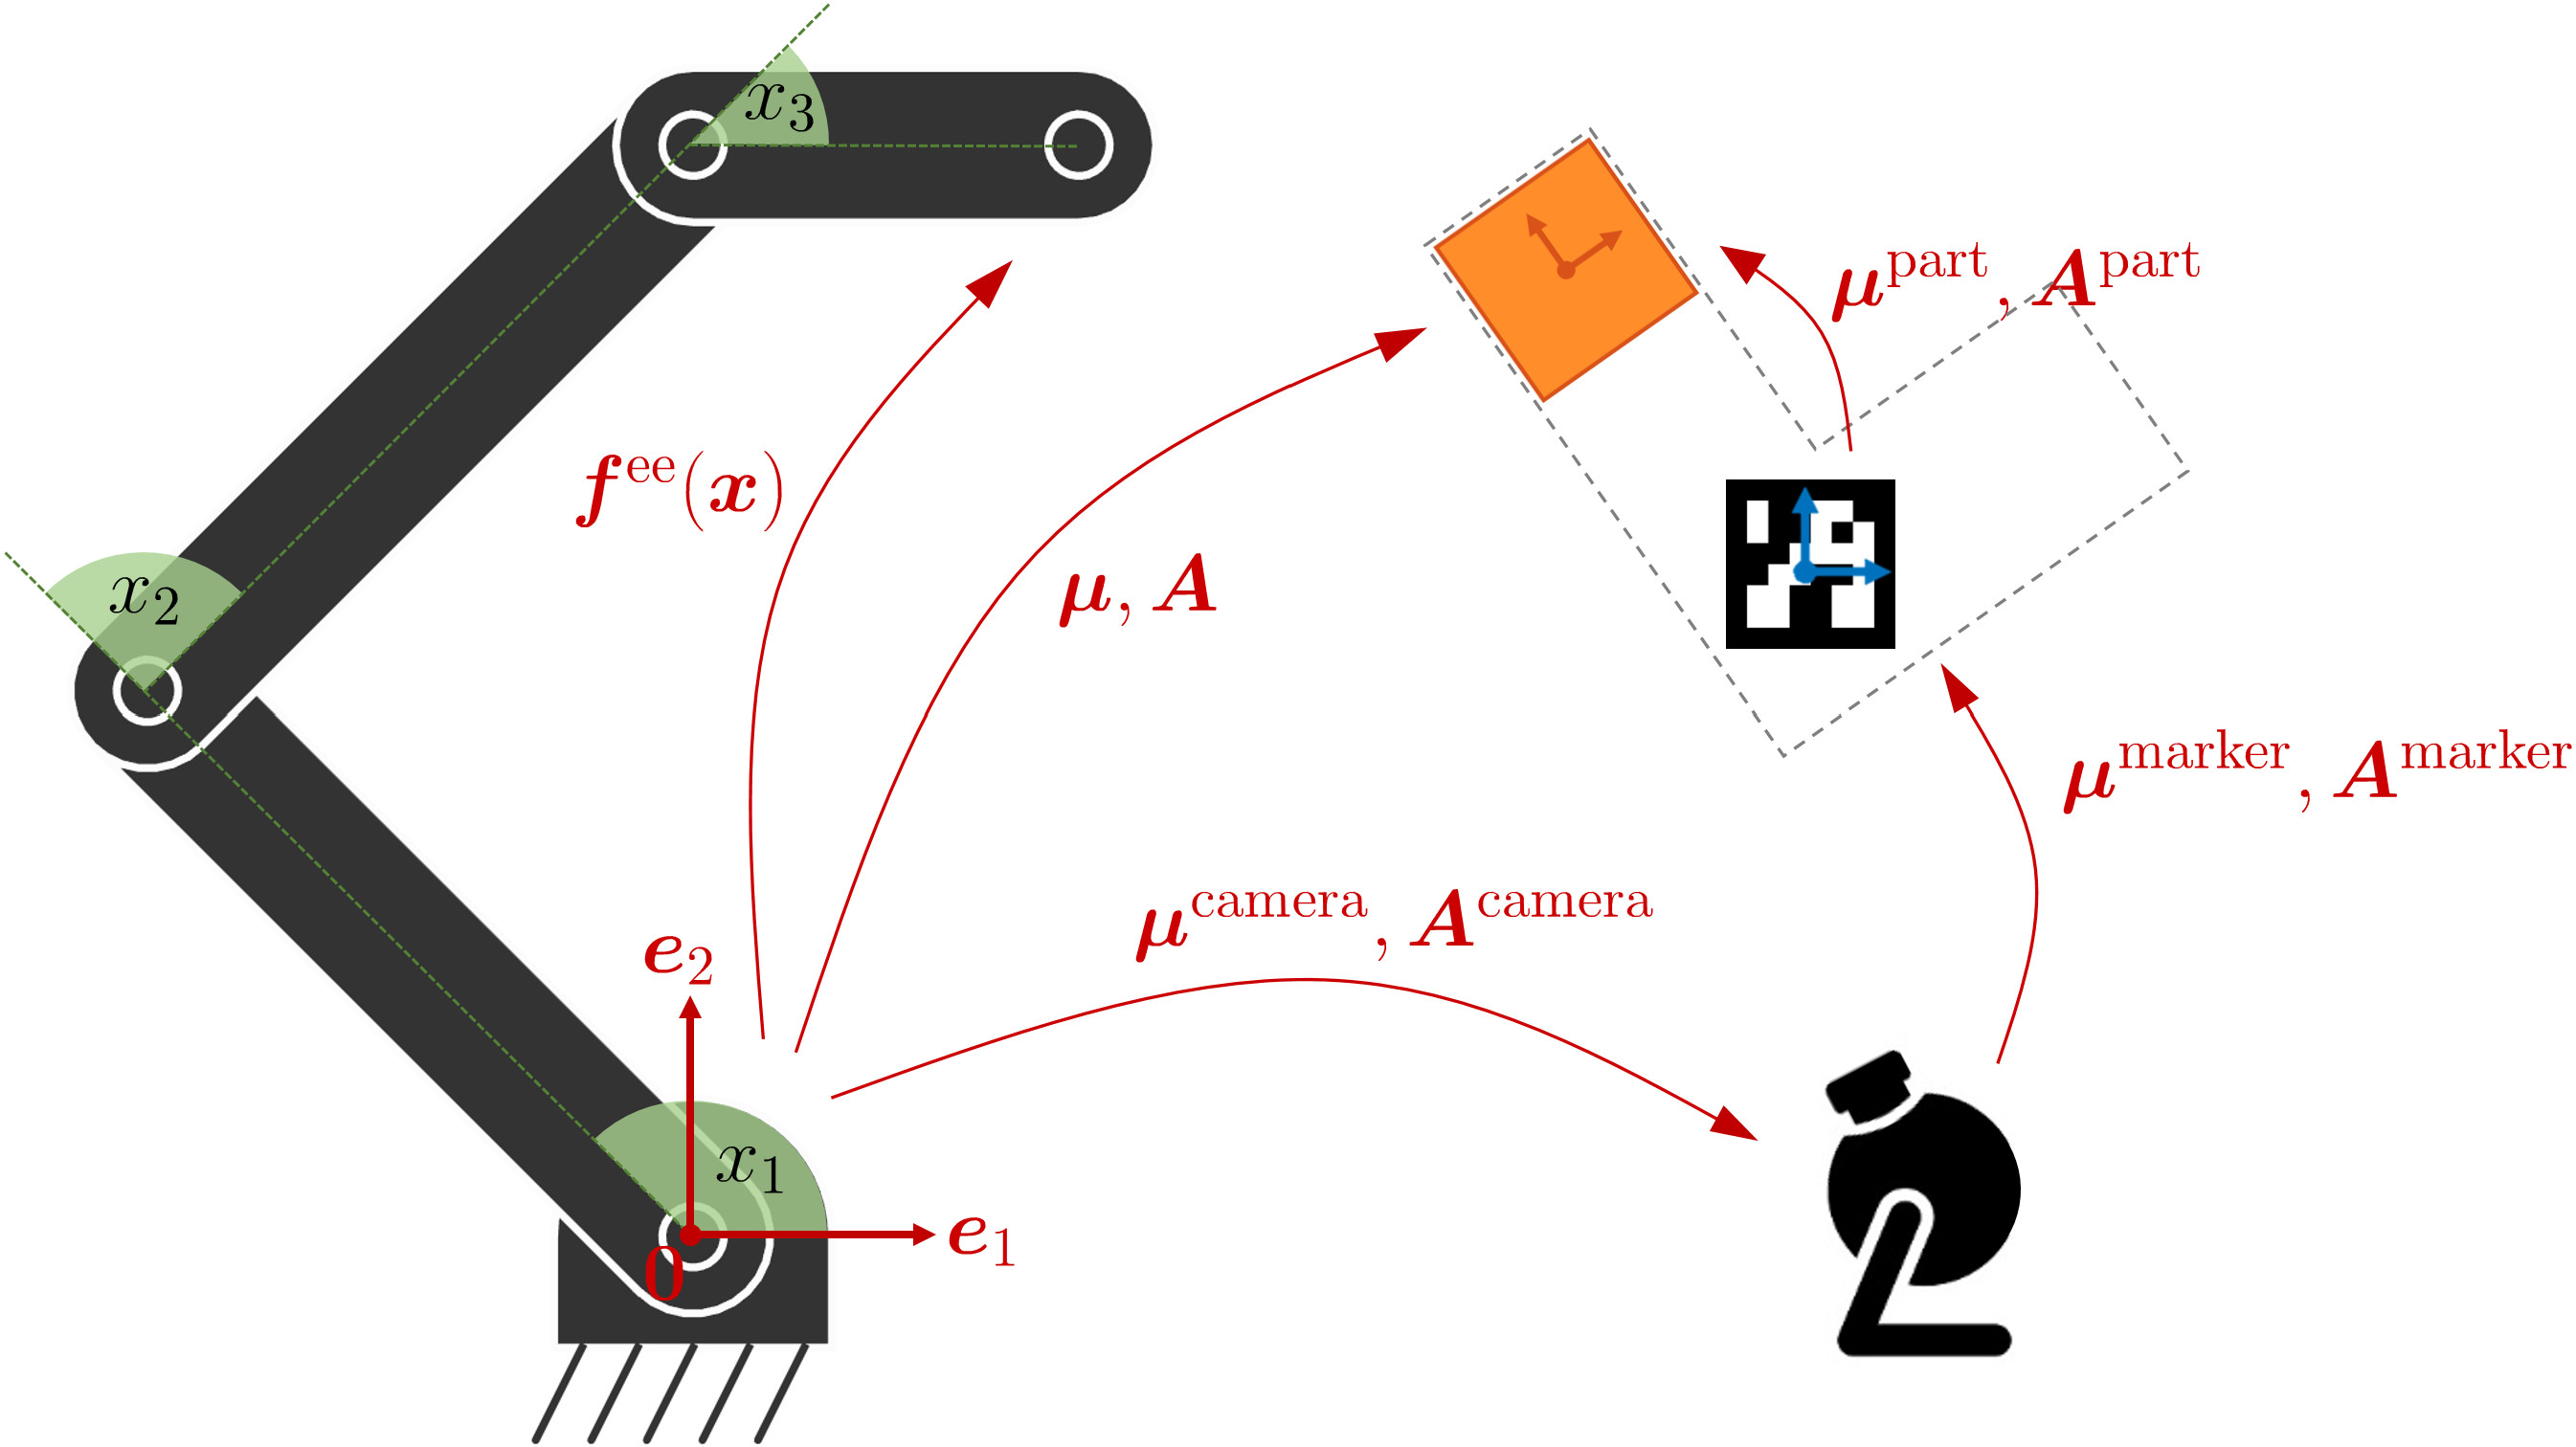
\includegraphics[width=.7\columnwidth]{images/transformations01.jpg}
\caption{\footnotesize
Typical transformations involved in a manipulation task involving a robot, a vision system, a visual marker on the object, and a desired grasping location on the object.  
}
\label{fig:transformations}
\end{figure}

We define a manipulation task involving a set of transformations as in Fig.~\ref{fig:transformations}. By relying on these transformation operators, we will next describe all variables in the robot frame of reference (defined by $\bm{0}$, $\bm{e}_1$ and $\bm{e}_2$ in the figure). 

For a manipulator controlled by joint angle velocity commands $\bm{u}=\bm{\dot{x}}$, the evolution of the system is described by $\bm{x}_{t+1} = \bm{x}_t + \bm{u}_t \Delta t$, with the Taylor expansion \eqref{eq:DS} simplifying to $\bm{A}_t=\frac{\partial\bm{g}}{\partial\bm{x}_t}=\bm{I}$ and $\bm{B}_t=\frac{\partial\bm{g}}{\partial\bm{u}_t}=\bm{I}\Delta t$. Similarly, a double integrator can alternatively be considered, with acceleration commands $\bm{u}=\bm{\ddot{x}}$ and states composed of both positions and velocities.

For a robot manipulator, $\bm{f}(\bm{x}_t)$ in \eqref{eq:du} typically represents the error between a reference $\bm{\mu}_t$ and the end-effector position computed by the forward kinematics function $\bm{f}^\tp{ee}(\bm{x}_t)$. We then have
\begin{align*}
	\bm{f}(\bm{x}_t) &= \bm{f}^\tp{ee}(\bm{x}_t) - \bm{\mu}_t, \\
	\bm{J}(\bm{x}_t) &= \bm{J}^\tp{ee}(\bm{x}_t).
\end{align*}

For the orientation part of the data (if considered), the Euclidean distance vector $\bm{f}^\tp{ee}(\bm{x}_t) - \bm{\mu}_t$ is replaced by a geodesic distance measure computed with the logarithmic map $\log_{\bm{\mu}_t}\!\big(\bm{f}^\tp{ee}(\bm{x}_t)\big)$, see \cite{Calinon20RAM} for details.

The approach can similarly be extended to target objects/landmarks with positions $\bm{\mu}_t$ and orientation matrices $\bm{U}_t$, whose columns are basis vectors forming a coordinate system, see Fig.~\ref{fig:iLQR_manipulator}. We can then define an error between the robot end-effector and an object/landmark expressed in the object/landmark coordinate system as 
\begin{equation}
\begin{aligned}
	\bm{f}(\bm{x}_t) &= \bm{U}_t^\trsp \big(\bm{f}^\tp{ee}(\bm{x}_t) - \bm{\mu}_t\big), \\
	\bm{J}(\bm{x}_t) &= \bm{U}_t^\trsp \bm{J}^\tp{ee}(\bm{x}_t). 
\end{aligned}
\label{eq:fJU}
\end{equation}


%%%%%%%%%%%%%%%%%%%%%%%%%%%%%%%%%%%%%%%%%%%%%%%%%%%%%%%%%%%%%%%%%%%%%%%%%%%%%%%%%
%\subsubsection{Bounded joint space}

%\begin{figure}
%\centering
%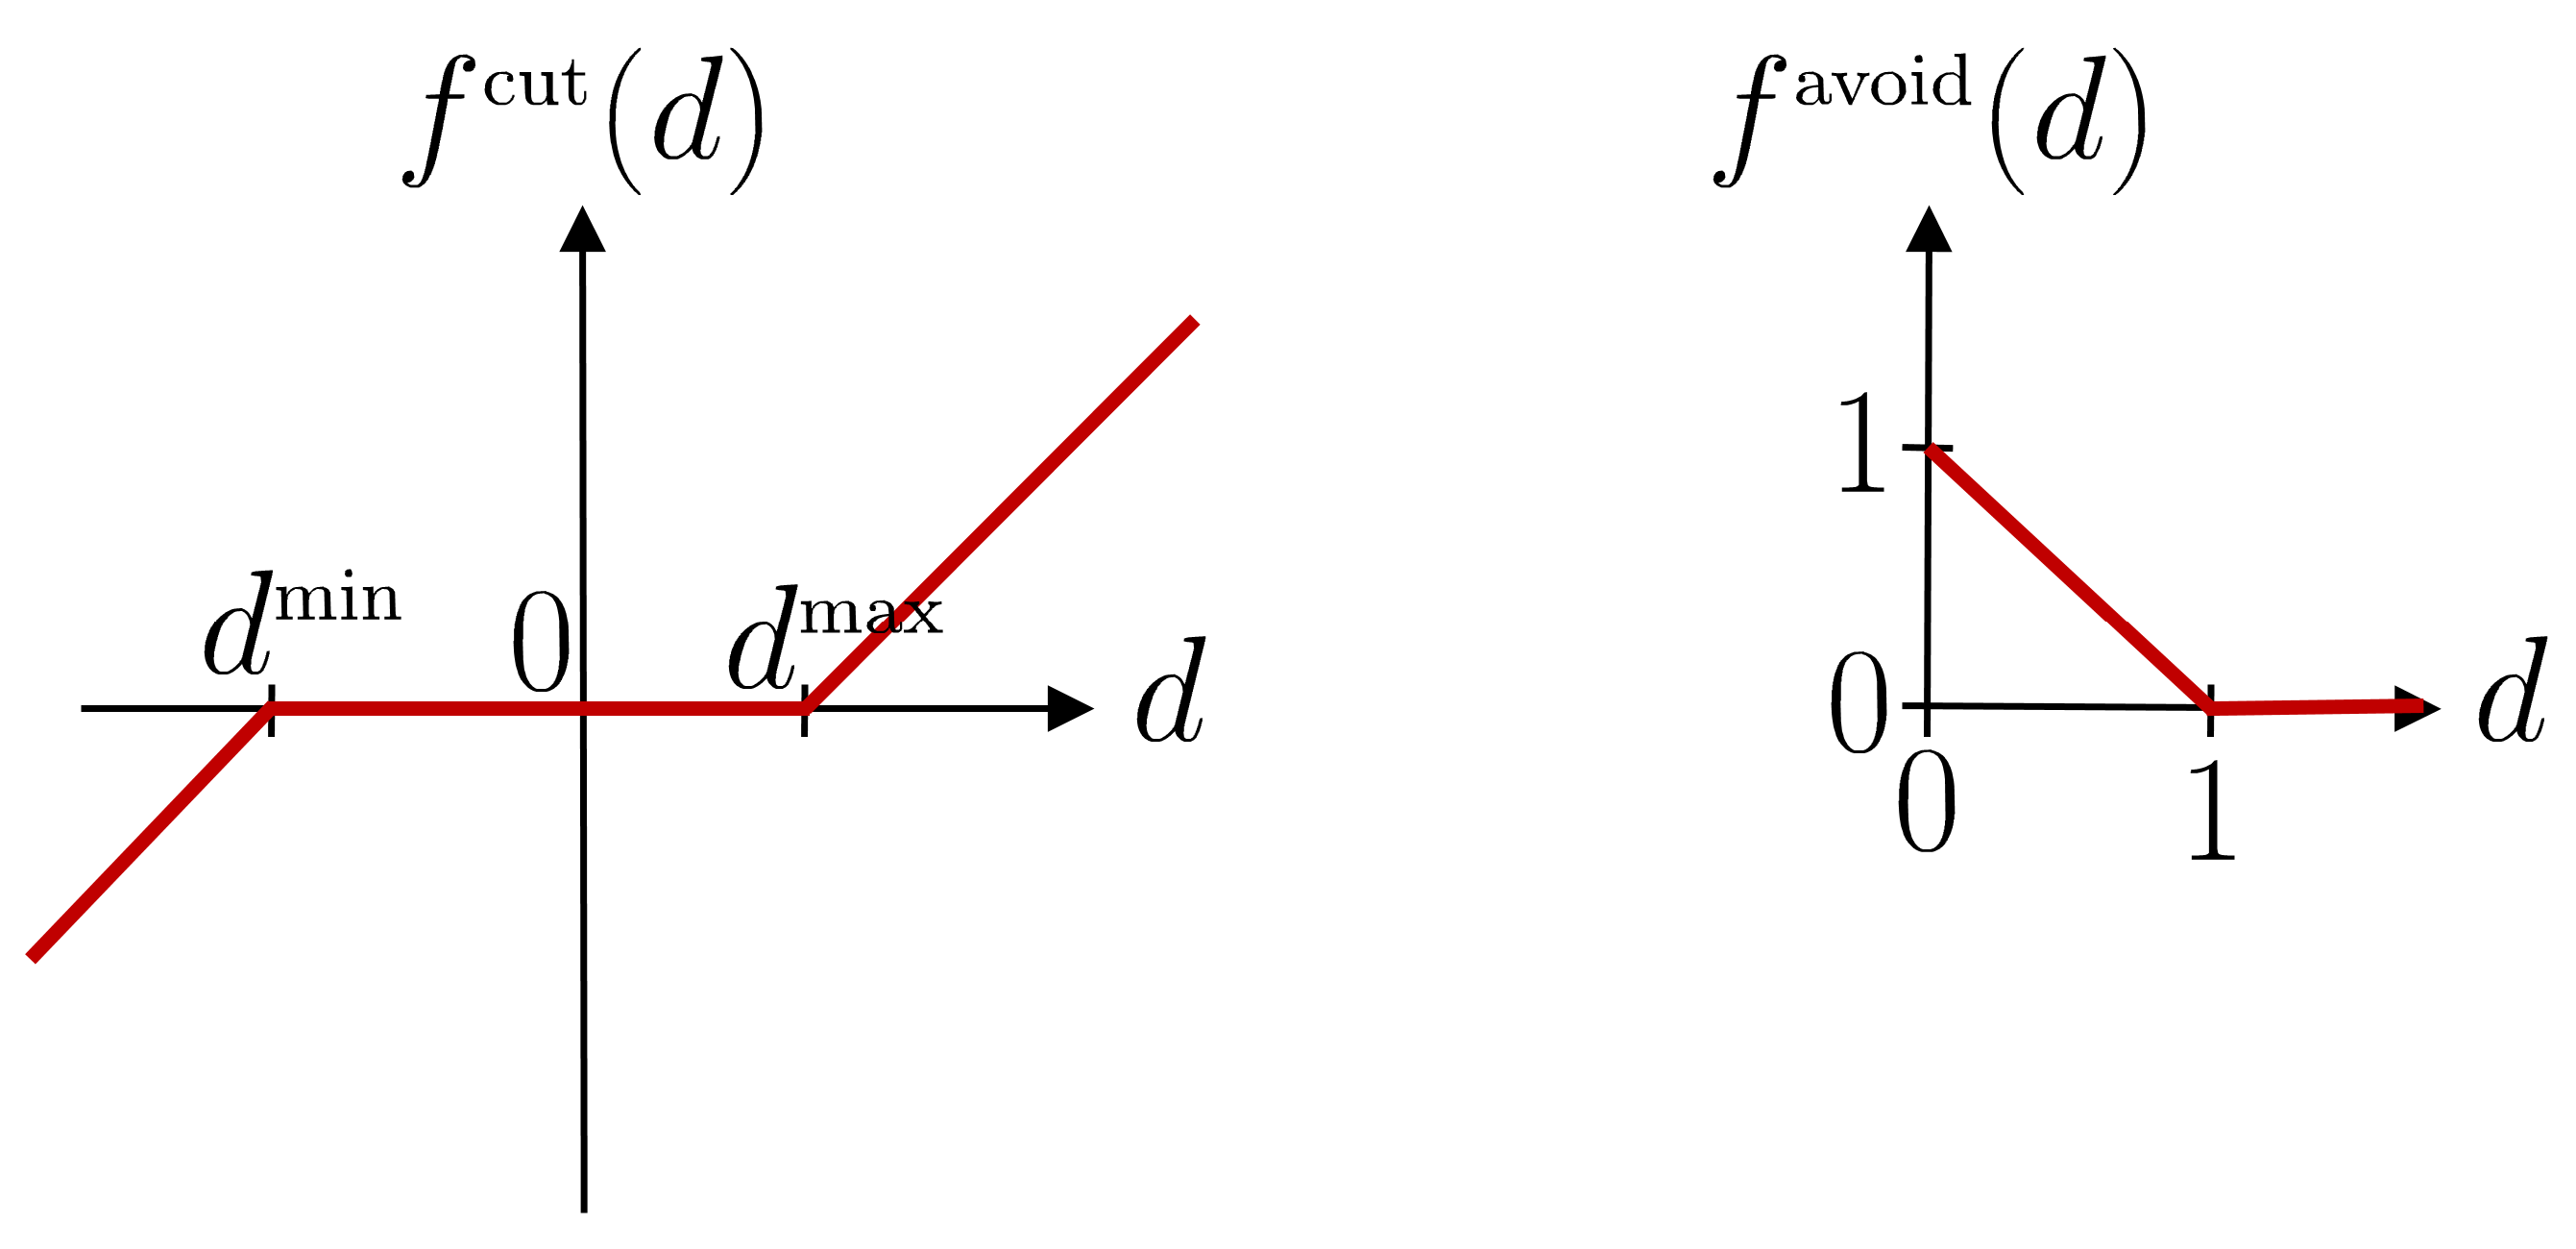
\includegraphics[width=.7\columnwidth]{images/fcut01.png}
%\caption{\footnotesize
%ReLU-like functions used in optimization costs. The derivatives of these functions are simple, providing Jacobians whose entries are either $0$ or $\pm 1$.  
%}
%\label{fig:fcut}
%\end{figure}

%The iLQR solution in \eqref{eq:du} can be used to keep the state within a boundary (e.g., joint angle limits). By using $\bm{f}(\bm{x})=\bm{f}^\tp{cut}(\bm{x})$ as the vertical concatenation of $\bm{f}^\tp{cut}(x_{t,i})$ and $\bm{J}(\bm{x})=\bm{J}^\tp{cut}(\bm{x})$ a diagonal Jacobian matrix with a diagonal concatenation of elements $\bm{J}^\tp{cut}_{t,i,i}$, we define
%\begin{align*}
%	\bm{f}^\tp{cut}(x_{t,i}) &= \begin{cases} 0, & \text{if}\ |x_{t,i}|<x_i^\tmax \\ x_{t,i} - \text{sgn}(x_{t,i}) x_i^\tmax, & \text{otherwise} \end{cases},\\
%	\bm{J}^\tp{cut}_{t,i,i} &= \begin{cases} 0,\hspace{27mm} & \text{if}\ |x_{t,i}|<x_i^\tmax \\ 1, & \text{otherwise} \end{cases},
%\end{align*}
%where $\bm{f}^\tp{cut}(x_{t,i})$ describe continuous ReLU-like functions for each dimension. $\bm{f}^\tp{cut}(x_{t,i})$ is $0$ inside the bounded domain and takes the signed distance value outside the boundary, see Fig.~\ref{fig:fcut}-\emph{left}.

%We can see with \eqref{eq:dcdx} that for $\bm{Q}=\frac{1}{2}\bm{I}$, if $\bm{x}$ is outside the domain during some time steps $t$ and for some dimension $i$, $\bm{g}_{\bm{x}} = \frac{\partial c}{\partial\bm{x}} = 2 {\bm{J}}^\trsp \bm{Q} \bm{f}$ generates a vector bringing it back to the boundary of the domain.


%%%%%%%%%%%%%%%%%%%%%%%%%%%%%%%%%%%%%%%%%%%%%%%%%%%%%%%%%%%%%%%%%%%%%%%%%%%%%%%%%
\subsubsection{Bounded joint space}

%\begin{figure}
%\centering
%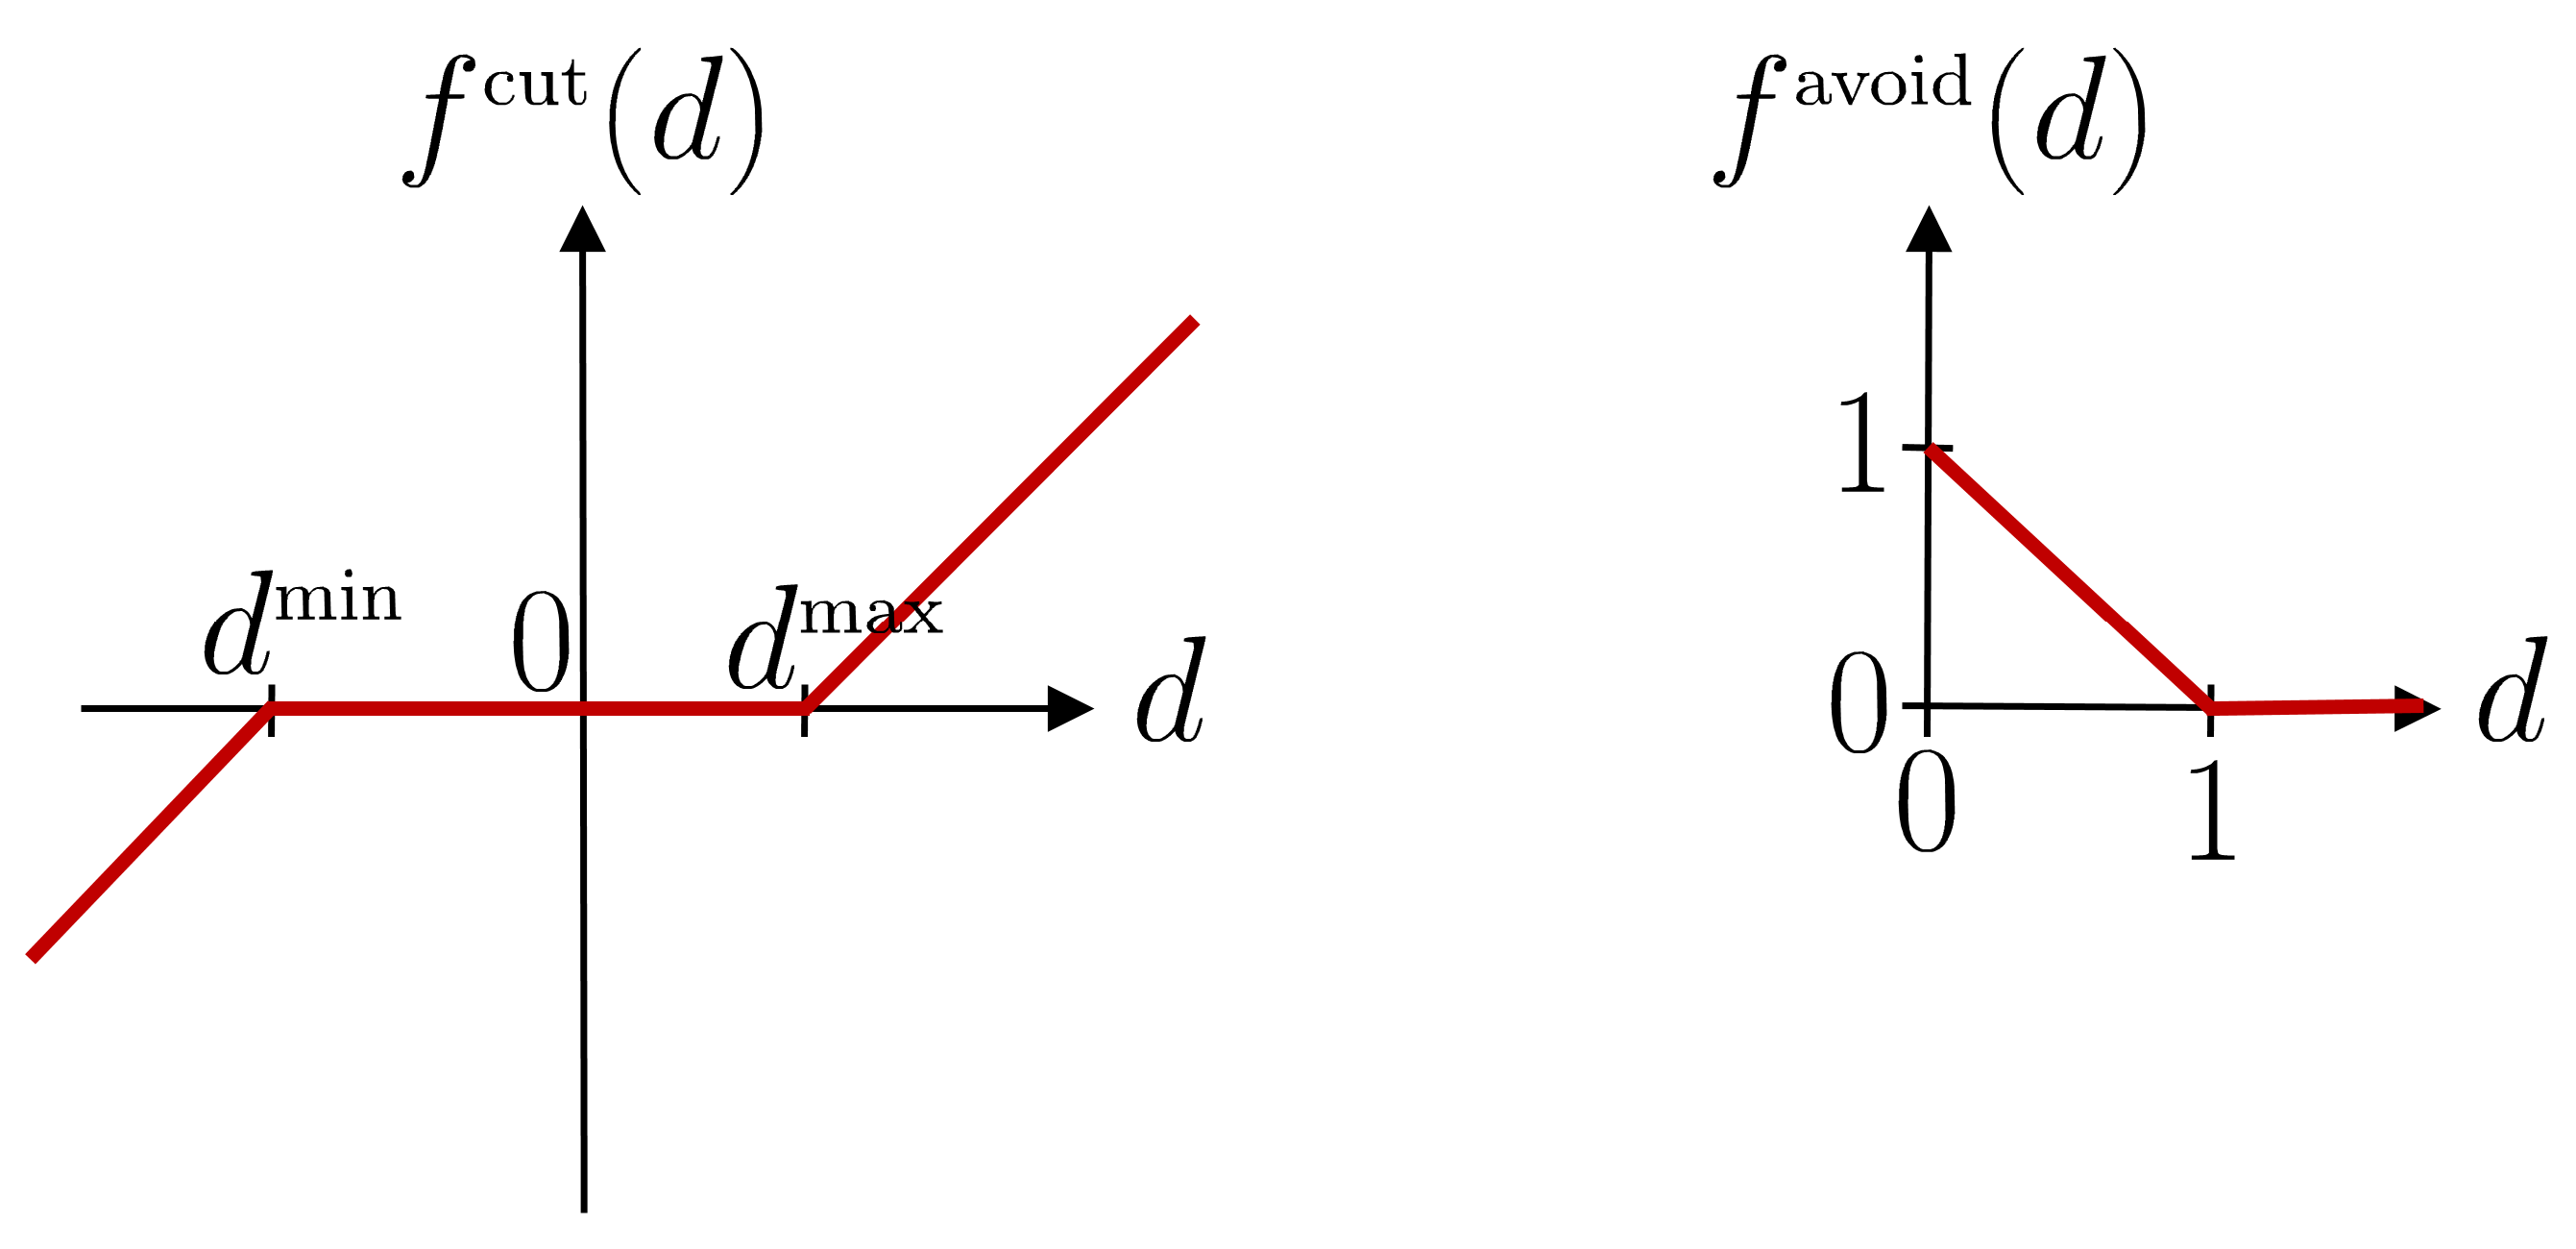
\includegraphics[width=.7\columnwidth]{images/fcut01.png}
%\caption{\footnotesize
%ReLU-like functions used in optimization costs. The derivatives of these functions are simple, providing Jacobians whose entries are either $0$ or $\pm 1$.  
%}
%\label{fig:fcut}
%\end{figure}

\begin{wrapfigure}{r}{.36\textwidth}
\vspace{-20pt}
\centering
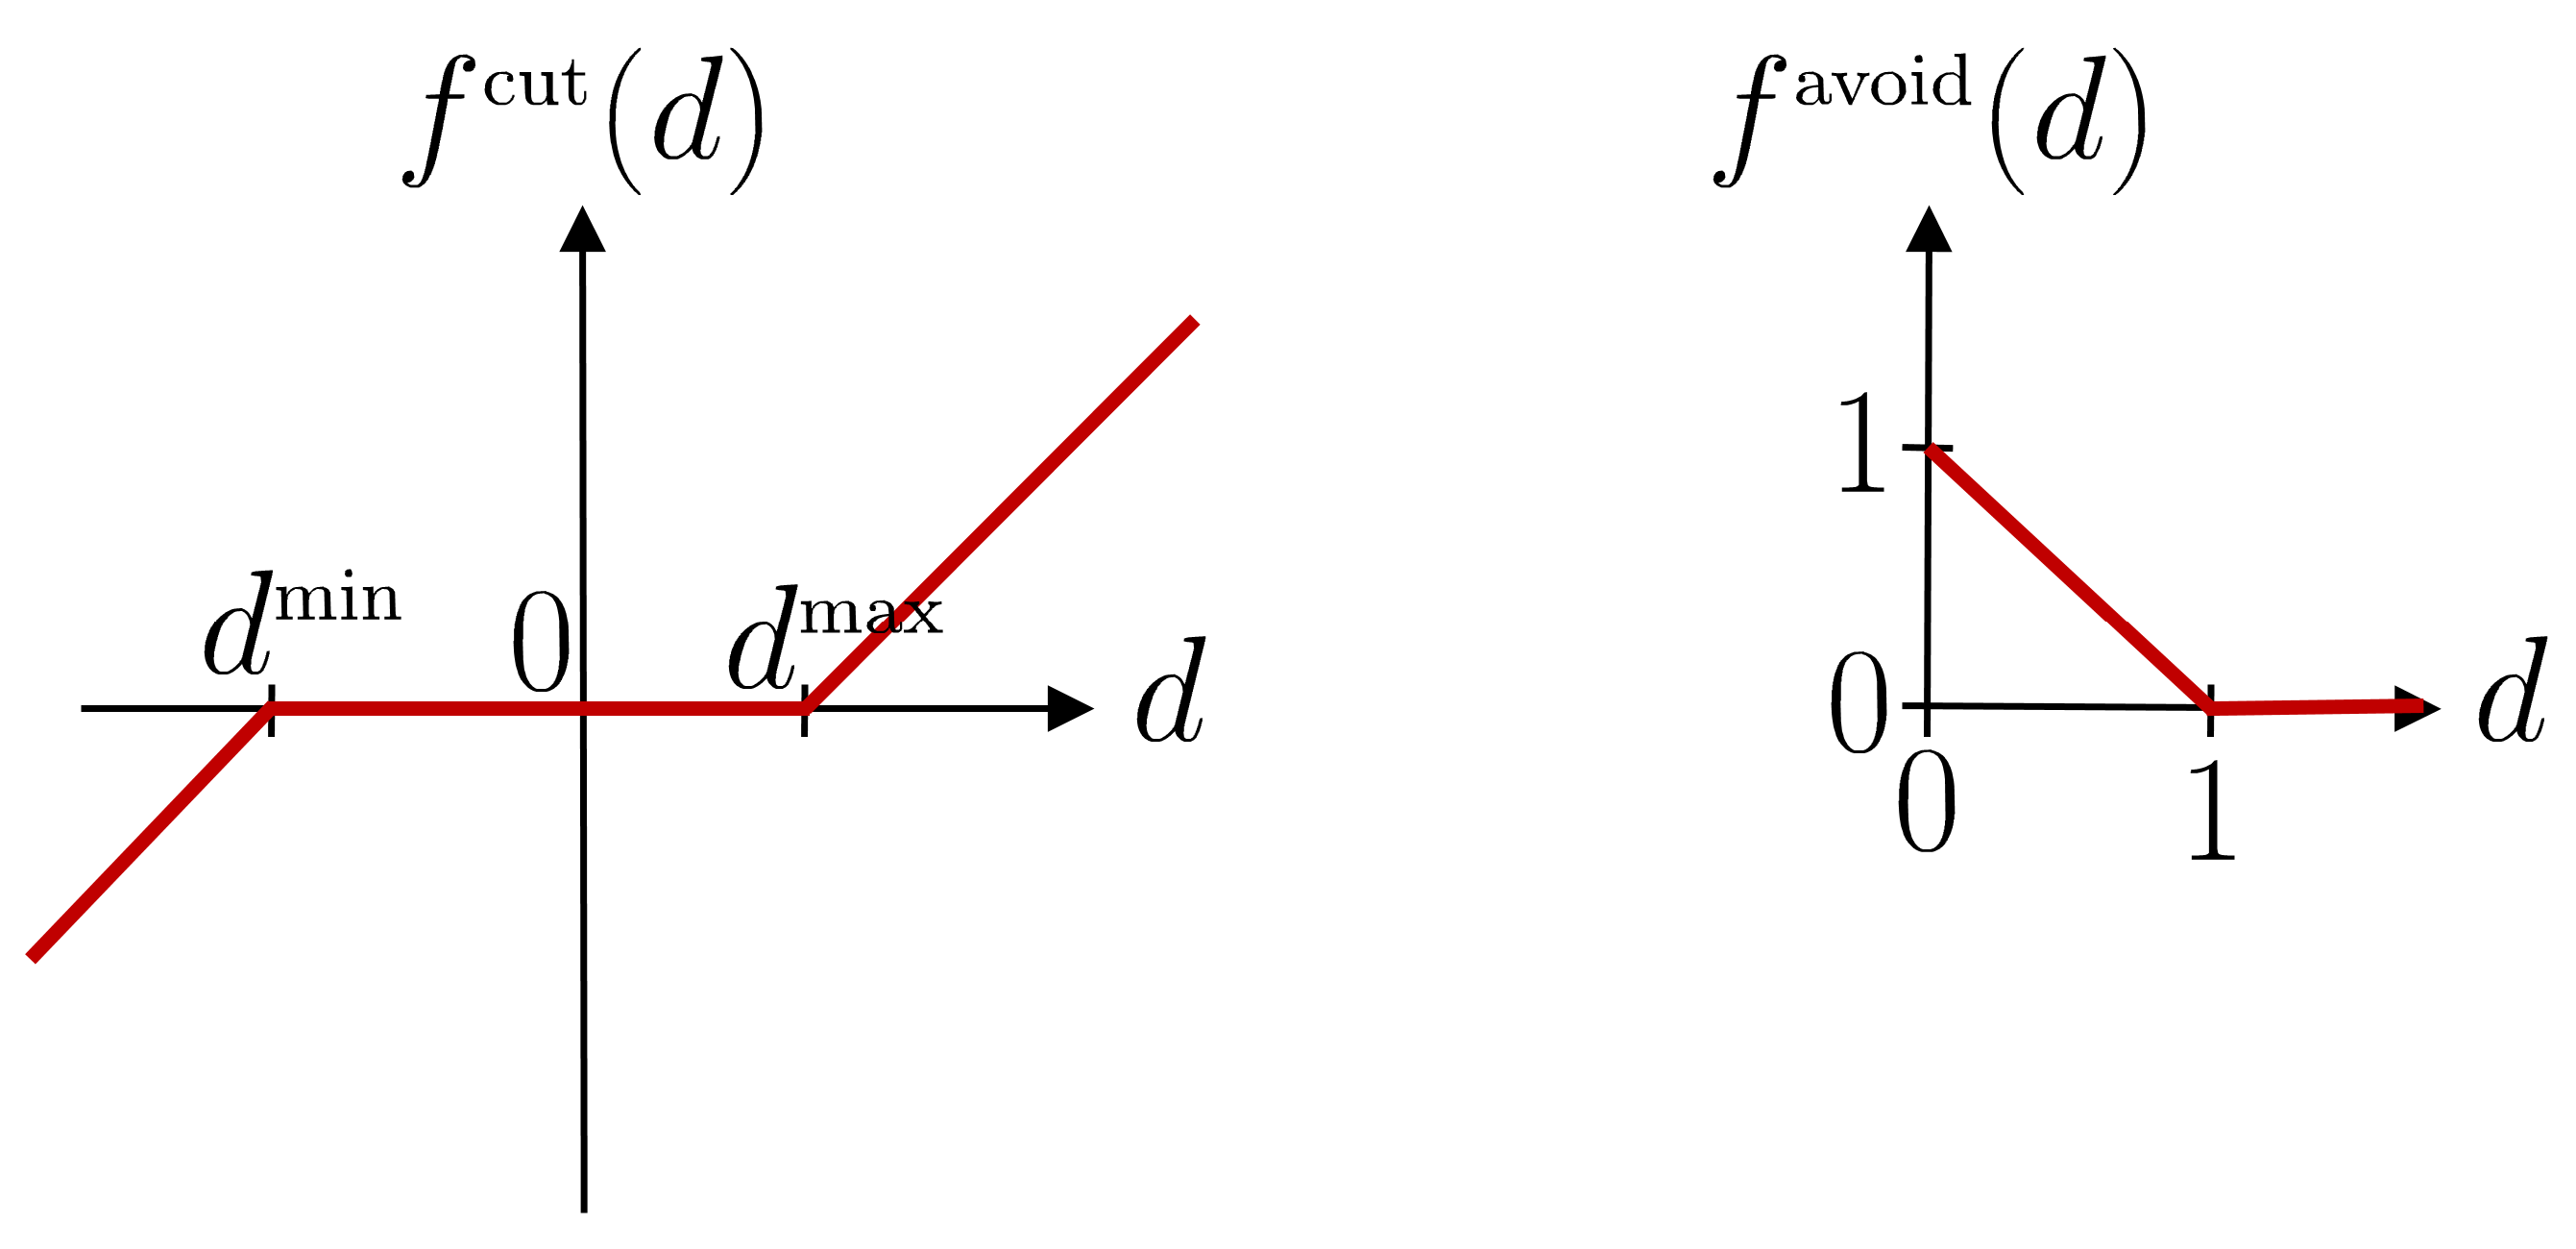
\includegraphics[width=.34\textwidth]{images/fcut01.png}
\caption{\footnotesize
ReLU-like functions used in optimization costs. The derivatives of these functions are simple, providing Jacobians whose entries are either $0$ or $\pm 1$.
}
\label{fig:fcut}
\vspace{-60pt}
\end{wrapfigure}

The iLQR solution in \eqref{eq:du} can be used to keep the state within a boundary (e.g., joint angle limits). We denote $\bm{f}(\bm{x})=\bm{f}^\tp{cut}(\bm{x})$ as the vertical concatenation of $\bm{f}^\tp{cut}(\bm{x}_t)$ and $\bm{J}(\bm{x})=\bm{J}^\tp{cut}(\bm{x})$ as a diagonal concatenation of diagonal Jacobian matrices $\bm{J}^\tp{cut}(\bm{x}_t)$. Each element $i$ of $\bm{f}^\tp{cut}(\bm{x}_t)$ and $\bm{J}^\tp{cut}(\bm{x}_t)$ is defined as 
\begin{align*}
	f^\tp{cut}_i(x_{t,i}) &= 
	\begin{cases} 
	x_{t,i} - x_i^\tmin, & \text{if}\ x_{t,i} < x_i^\tmin \\
	x_{t,i} - x_i^\tmax, & \text{if}\ x_{t,i} > x_i^\tmax \\
	0, & \text{otherwise} 
	\end{cases},\\
	J^\tp{cut}_{i,i}(x_{t,i}) &= 
	\begin{cases} 
	1,\hspace{14mm} & \text{if}\ x_{t,i} < x_i^\tmin \\
	1, & \text{if}\ x_{t,i} > x_i^\tmax \\
	0, & \text{otherwise} 
	\end{cases},
\end{align*}
where $f^\tp{cut}_i(x_{t,i})$ describes continuous ReLU-like functions for each dimension. $f^\tp{cut}_i(x_{t,i})$ is $0$ inside the bounded domain and takes the signed distance value outside the boundary, see Fig.~\ref{fig:fcut}-\emph{left}.

We can see with \eqref{eq:dcdx} that for $\bm{Q}=\frac{1}{2}\bm{I}$, if $\bm{x}$ is outside the domain during some time steps $t$, $\bm{g}_{\bm{x}} = \frac{\partial c}{\partial\bm{x}} = 2 {\bm{J}}^\trsp \bm{Q} \bm{f}$ generates a vector bringing it back to the boundary of the domain.


%%%%%%%%%%%%%%%%%%%%%%%%%%%%%%%%%%%%%%%%%%%%%%%%%%%%%%%%%%%%%%%%%%%%%%%%%%%%%%%%%
\subsubsection{Bounded task space}

The iLQR solution in \eqref{eq:du} can be used to keep the end-effector within a boundary (e.g., end-effector position limits).
Based on the above definitions, $\bm{f}(\bm{x})$ and $\bm{J}(\bm{x})$ are in this case defined as
\begin{align*}
	\bm{f}(\bm{x}_t) &= \bm{f}^\tp{cut}\Big(\bm{e}(\bm{x}_t)\Big), \\
	\bm{J}(\bm{x}_t) &= \bm{J}^\tp{cut}\Big(\bm{e}(\bm{x}_t)\Big) \; \bm{J}^\tp{ee}(\bm{x}_t), \\
	\text{with}\quad \bm{e}(\bm{x}_t) &= \bm{f}^\tp{ee}(\bm{x}_t).
\end{align*}
%\bm{y}

\begin{SCfigure}
\centering
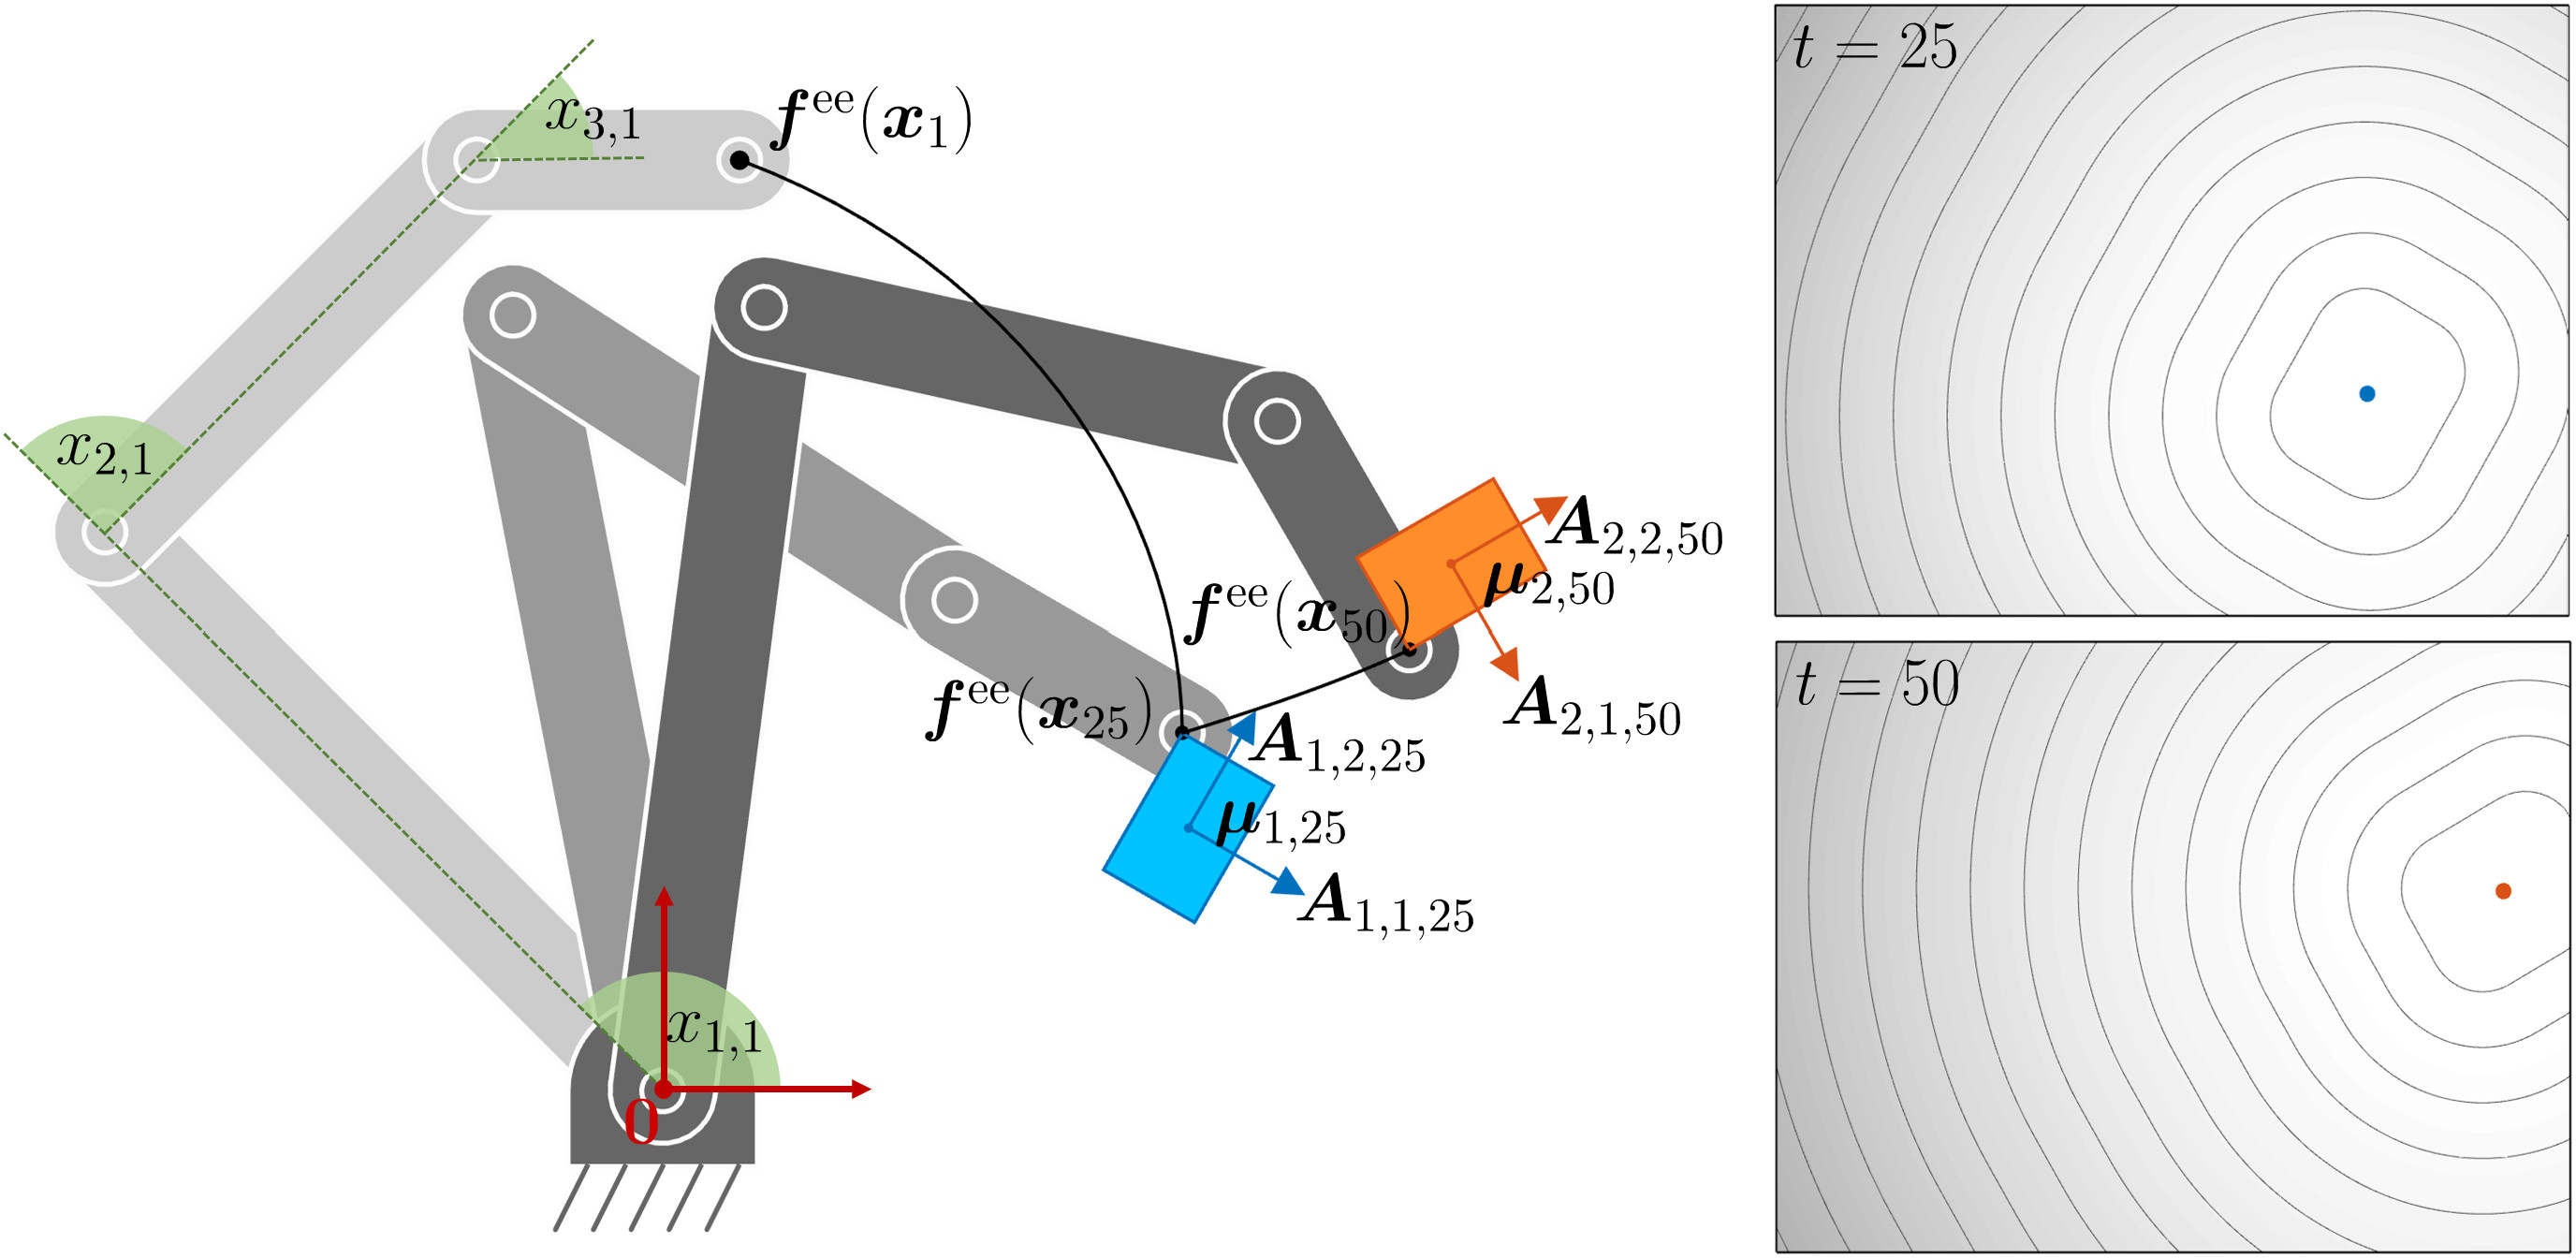
\includegraphics[width=.6\textwidth]{images/iLQR_objectBoundaries01.jpg}
\caption{\footnotesize
Example of a viapoints task in which a planar robot with 3 joints needs to sequentially reach 2 objects, with object boundaries defining the allowed reaching points on the objects surfaces. \emph{Left:} Reaching task with two viapoints at $t=25$ and $t=50$. \emph{Right:} Corresponding values of the cost function for the end-effector space at $t=25$ and $t=50$.
}
\label{fig:iLQR_manipulator}
\end{SCfigure}


%%%%%%%%%%%%%%%%%%%%%%%%%%%%%%%%%%%%%%%%%%%%%%%%%%%%%%%%%%%%%%%%%%%%%%%%%%%%%%%%%
\subsubsection{Reaching task with robot manipulator and prismatic object boundaries}\label{sec:reaching}
\begin{flushright}
\filename{iLQR\_manipulator.*}
\end{flushright}

The definition of $\bm{f}(\bm{x}_t)$ and $\bm{J}(\bm{x}_t)$ in \eqref{eq:fJU} can also be extended to objects/landmarks with boundaries by defining
\begin{align*}
	\bm{f}(\bm{x}_t) &= \bm{f}^\tp{cut}\Big( \bm{e}(\bm{x}_t) \Big), \\
	\bm{J}(\bm{x}_t) &= \bm{J}^\tp{cut}\Big( \bm{e}(\bm{x}_t) \Big) \; \bm{U}_t^\trsp \; \bm{J}^\tp{ee}(\bm{x}_t), \\
	\text{with}\quad \bm{e}(\bm{x}_t) &= \bm{U}_t^\trsp \big(\bm{f}^\tp{ee}(\bm{x}_t) - \bm{\mu}_t\big),
\end{align*}
see also Fig.~\ref{fig:iLQR_manipulator}.

%% Can a similar approach be used for prismatic object avoidance?


%%%%%%%%%%%%%%%%%%%%%%%%%%%%%%%%%%%%%%%%%%%%%%%%%%%%%%%%%%%%%%%%%%%%%%%%%%%%%%%%%%
%\subsubsection{Initial pose estimation}\label{sec:initialPose}
%\begin{flushright}
%\filename{iLQR\_manipulator.*}
%\end{flushright}



%%%%%%%%%%%%%%%%%%%%%%%%%%%%%%%%%%%%%%%%%%%%%%%%%%%%%%%%%%%%%%%%%%%%%%%%%%%%%%%%%
\subsubsection{Center of mass}
\begin{flushright}
\filename{iLQR\_manipulator\_CoM.*}
\end{flushright}

%\begin{figure}
%\centering
%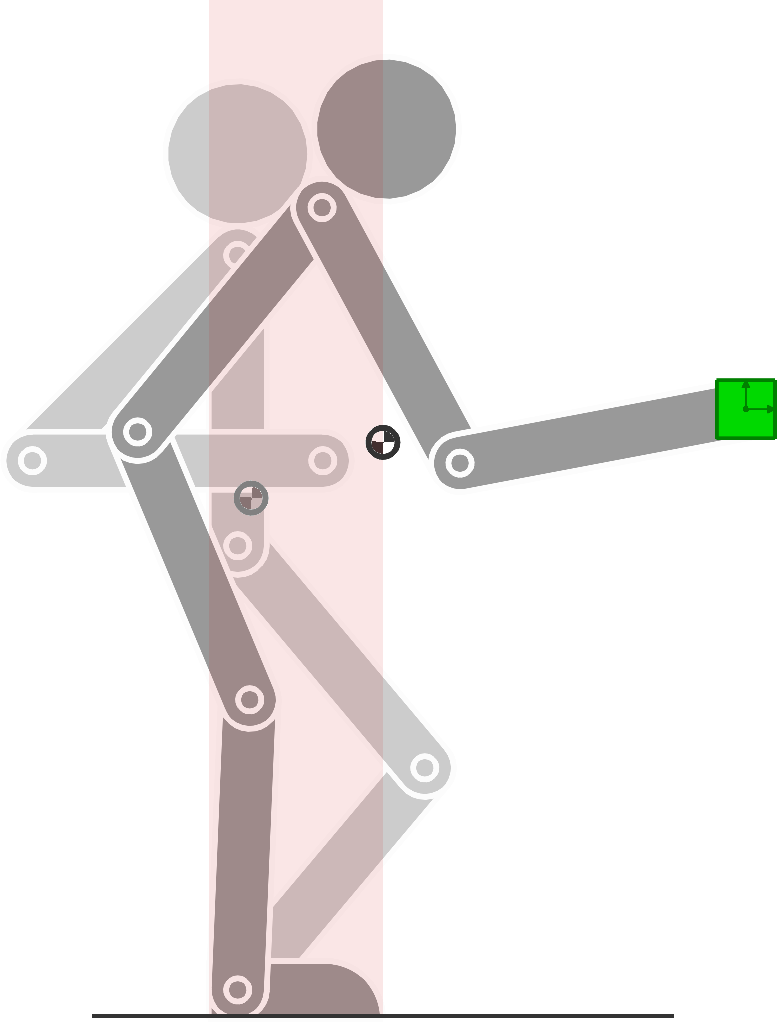
\includegraphics[width=.3\textwidth]{images/iLQR_CoM01.png}
%\caption{\footnotesize
%Reaching task with a humanoid (side view) by keeping the center of mass in an area defined by the feet location. The starting and ending poses are depicted in different grayscale levels. The corresponding center of mass is depicted by a darker semi-filled disc. The area allowed for the center of mass is depicted as a transparent red rectangle. The task consists of reaching the green object with the end-effector at the end of the movement, while always keeping the center of mass within the desired bounding box during the movement.
%}
%\label{fig:iLQR_CoM}
%\end{figure}

%\begin{SCfigure}[50]
%\centering
%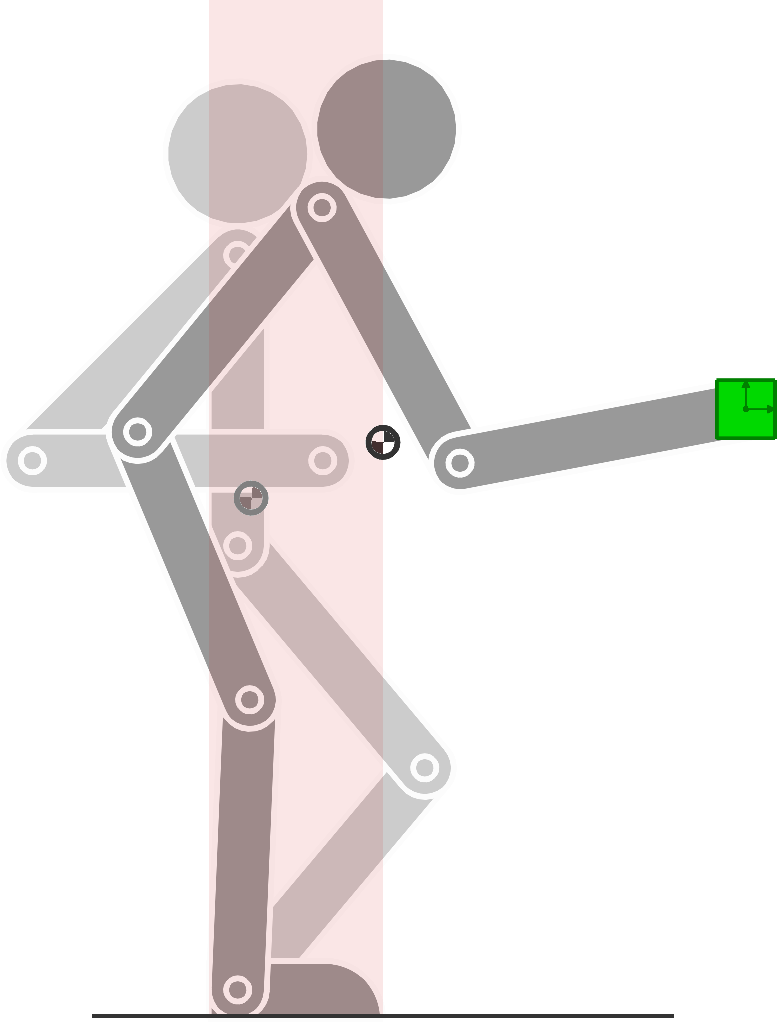
\includegraphics[width=.25\textwidth]{images/iLQR_CoM01.png}
%\caption{\footnotesize
%Reaching task with a humanoid (side view) by keeping the center of mass in an area defined by the feet location. The starting and ending poses are depicted in different grayscale levels. The corresponding center of mass is depicted by a darker semi-filled disc. The area allowed for the center of mass is depicted as a transparent red rectangle. The task consists of reaching the green object with the end-effector at the end of the movement, while always keeping the center of mass within the desired bounding box during the movement.
%}
%\label{fig:iLQR_CoM}
%\end{SCfigure}

\begin{wrapfigure}{r}{.30\textwidth}
%\vspace{-20pt}
\centering
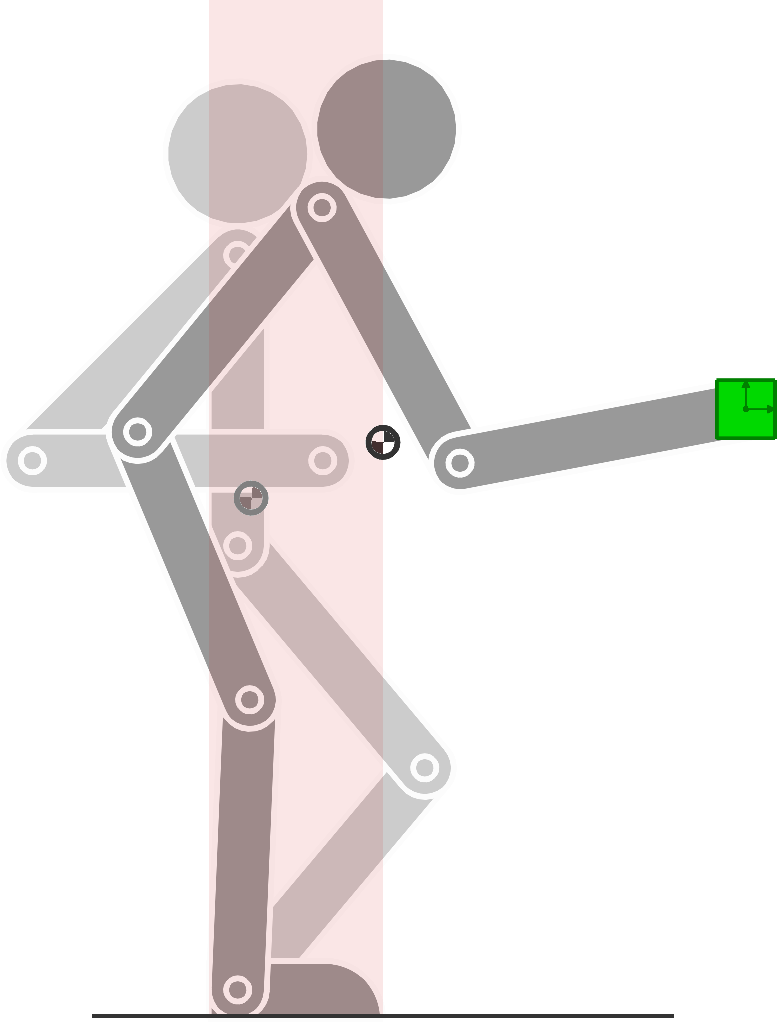
\includegraphics[width=.28\textwidth]{images/iLQR_CoM01.png}
\caption{\footnotesize
Reaching task with a humanoid (side view) by keeping the center of mass in an area defined by the feet location. 
}
\label{fig:iLQR_CoM}
\vspace{-20pt}
\end{wrapfigure}

If we assume an equal mass for each link concentrated at the joint (i.e., assuming that the motors and gripper are heavier than the link structures), the forward kinematics function to determine the center of a mass of an articulated chain can simply be computed with
\begin{equation*}
	\bm{f}^\tp{CoM} = \frac{1}{D}\begin{bmatrix} \bm{\ell}^\trsp \bm{L} \cos(\bm{L}\bm{x}) \\ \bm{\ell}^\trsp \bm{L} \sin(\bm{L}\bm{x}) \end{bmatrix},
\end{equation*}
which corresponds to the row average of $\tilde{f}$ in \eqref{eq:FKall} for the first two columns (position).	
%	f = [model.l' * L * cos(L * x); ...
%		 model.l' * L * sin(L * x)] / model.nbVarX;
The corresponding Jacobian matrix is
\begin{equation*}
	\bm{J}^\tp{CoM} = \frac{1}{D}\begin{bmatrix} 
	-\sin(\bm{L}\bm{x})^\trsp \bm{L} \; \diag(\bm{\ell}^\trsp \bm{L}) \\ 
	\cos(\bm{L}\bm{x})^\trsp \bm{L} \; \diag(\bm{\ell}^\trsp \bm{L})
	\end{bmatrix}.
\end{equation*}
%	Jtmp = [-sin(L * x(:,t))' * L * diag(model.l' * L); ...
%			 cos(L * x(:,t))' * L * diag(model.l' * L)] / model.nbVarX;

The forward kinematics function $\bm{f}^\tp{CoM}$ can be used in tracking tasks similar to the ones considering the end-effector, as in Section \ref{sec:reaching}. Fig.~\ref{fig:iLQR_CoM} shows an example in which the starting and ending poses are depicted in different grayscale levels. The corresponding center of mass is depicted by a darker semi-filled disc. The area allowed for the center of mass is depicted as a transparent red rectangle. The task consists of reaching the green object with the end-effector at the end of the movement, while always keeping the center of mass within the desired bounding box during the movement.



%%%%%%%%%%%%%%%%%%%%%%%%%%%%%%%%%%%%%%%%%%%%%%%%%%%%%%%%%%%%%%%%%%%%%%%%%%%%%%%%%
\subsubsection{Bimanual robot}
\begin{flushright}
\filename{iLQR\_bimanual.*}
\end{flushright}

\begin{SCfigure}%[40]
\centering
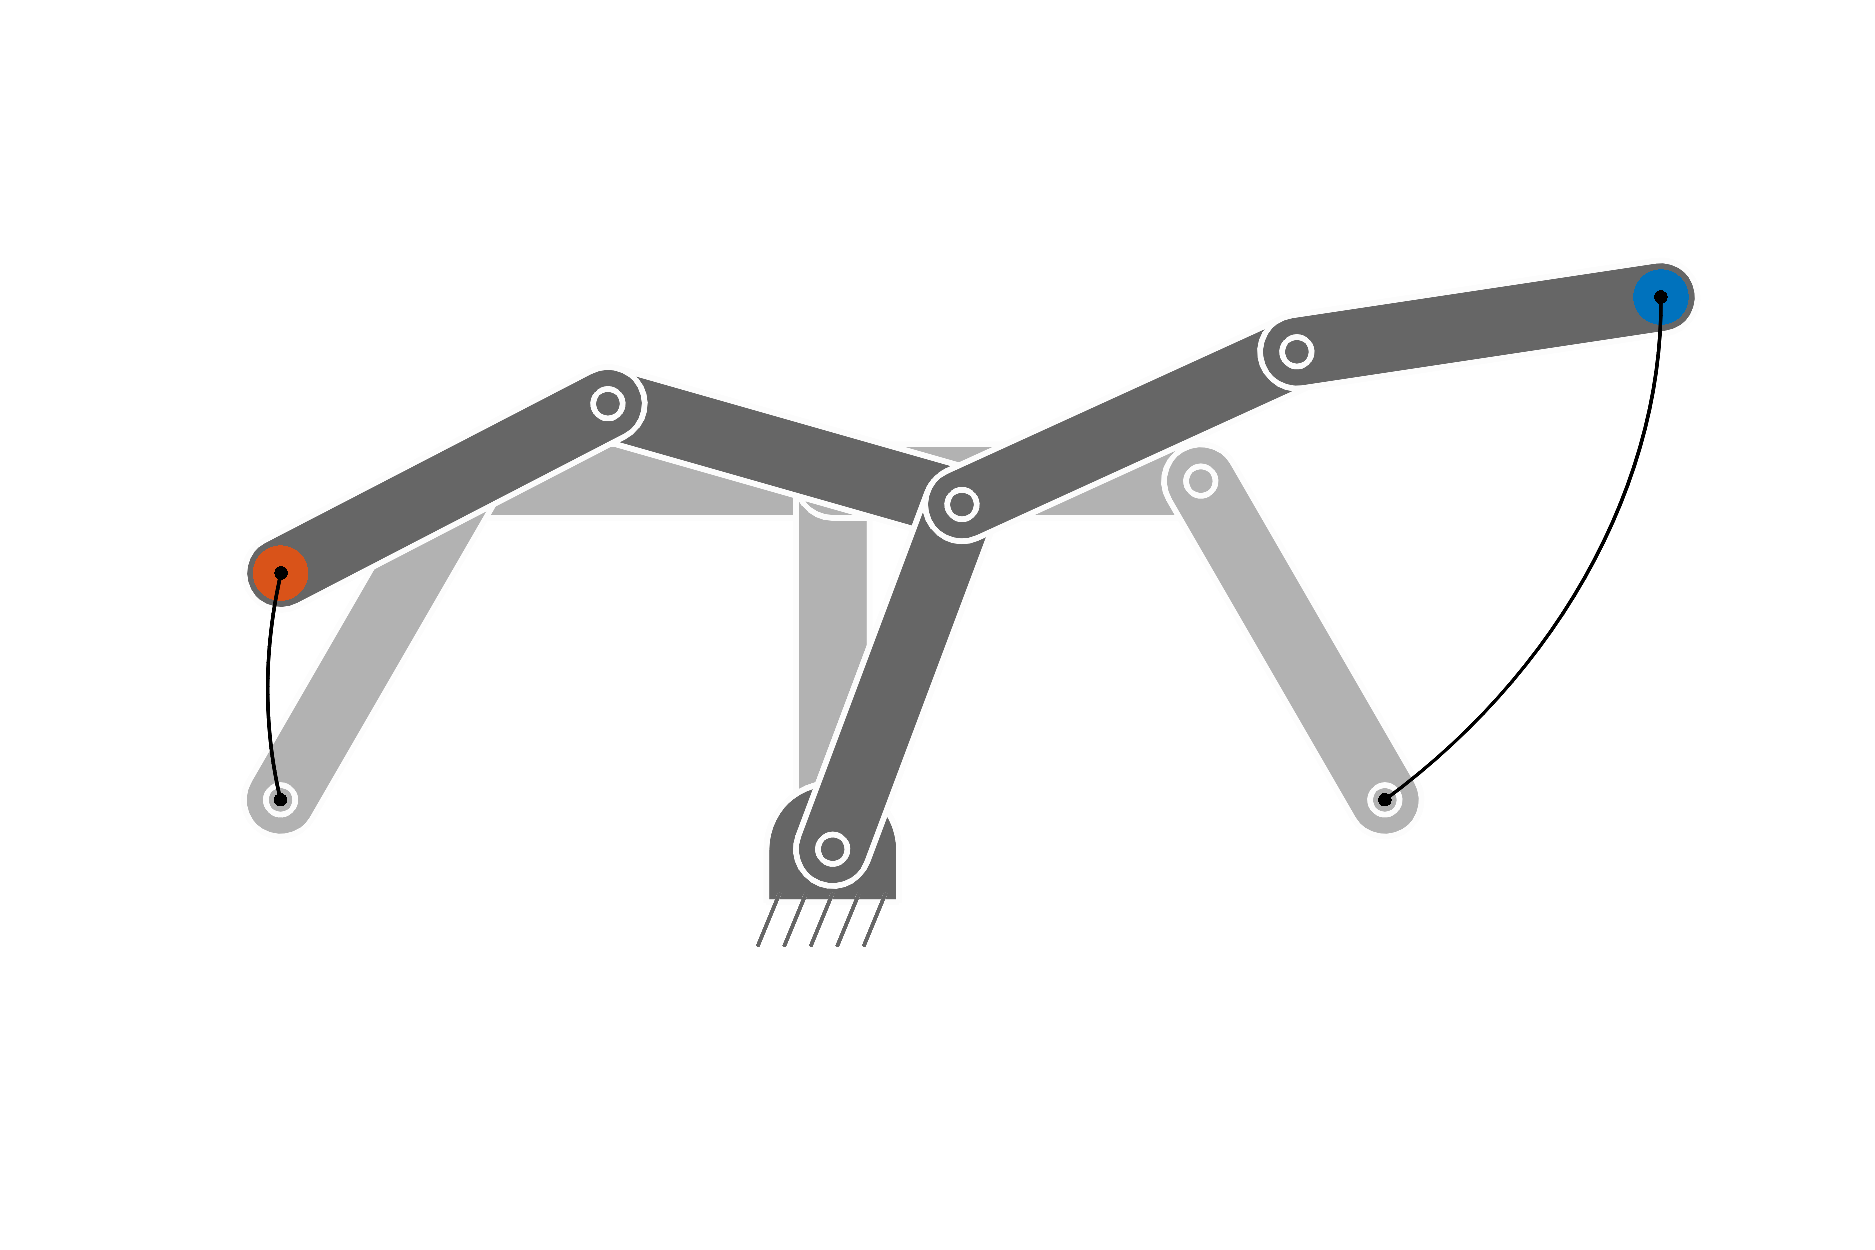
\includegraphics[width=.38\columnwidth]{images/iLQR_bimanual02.png}
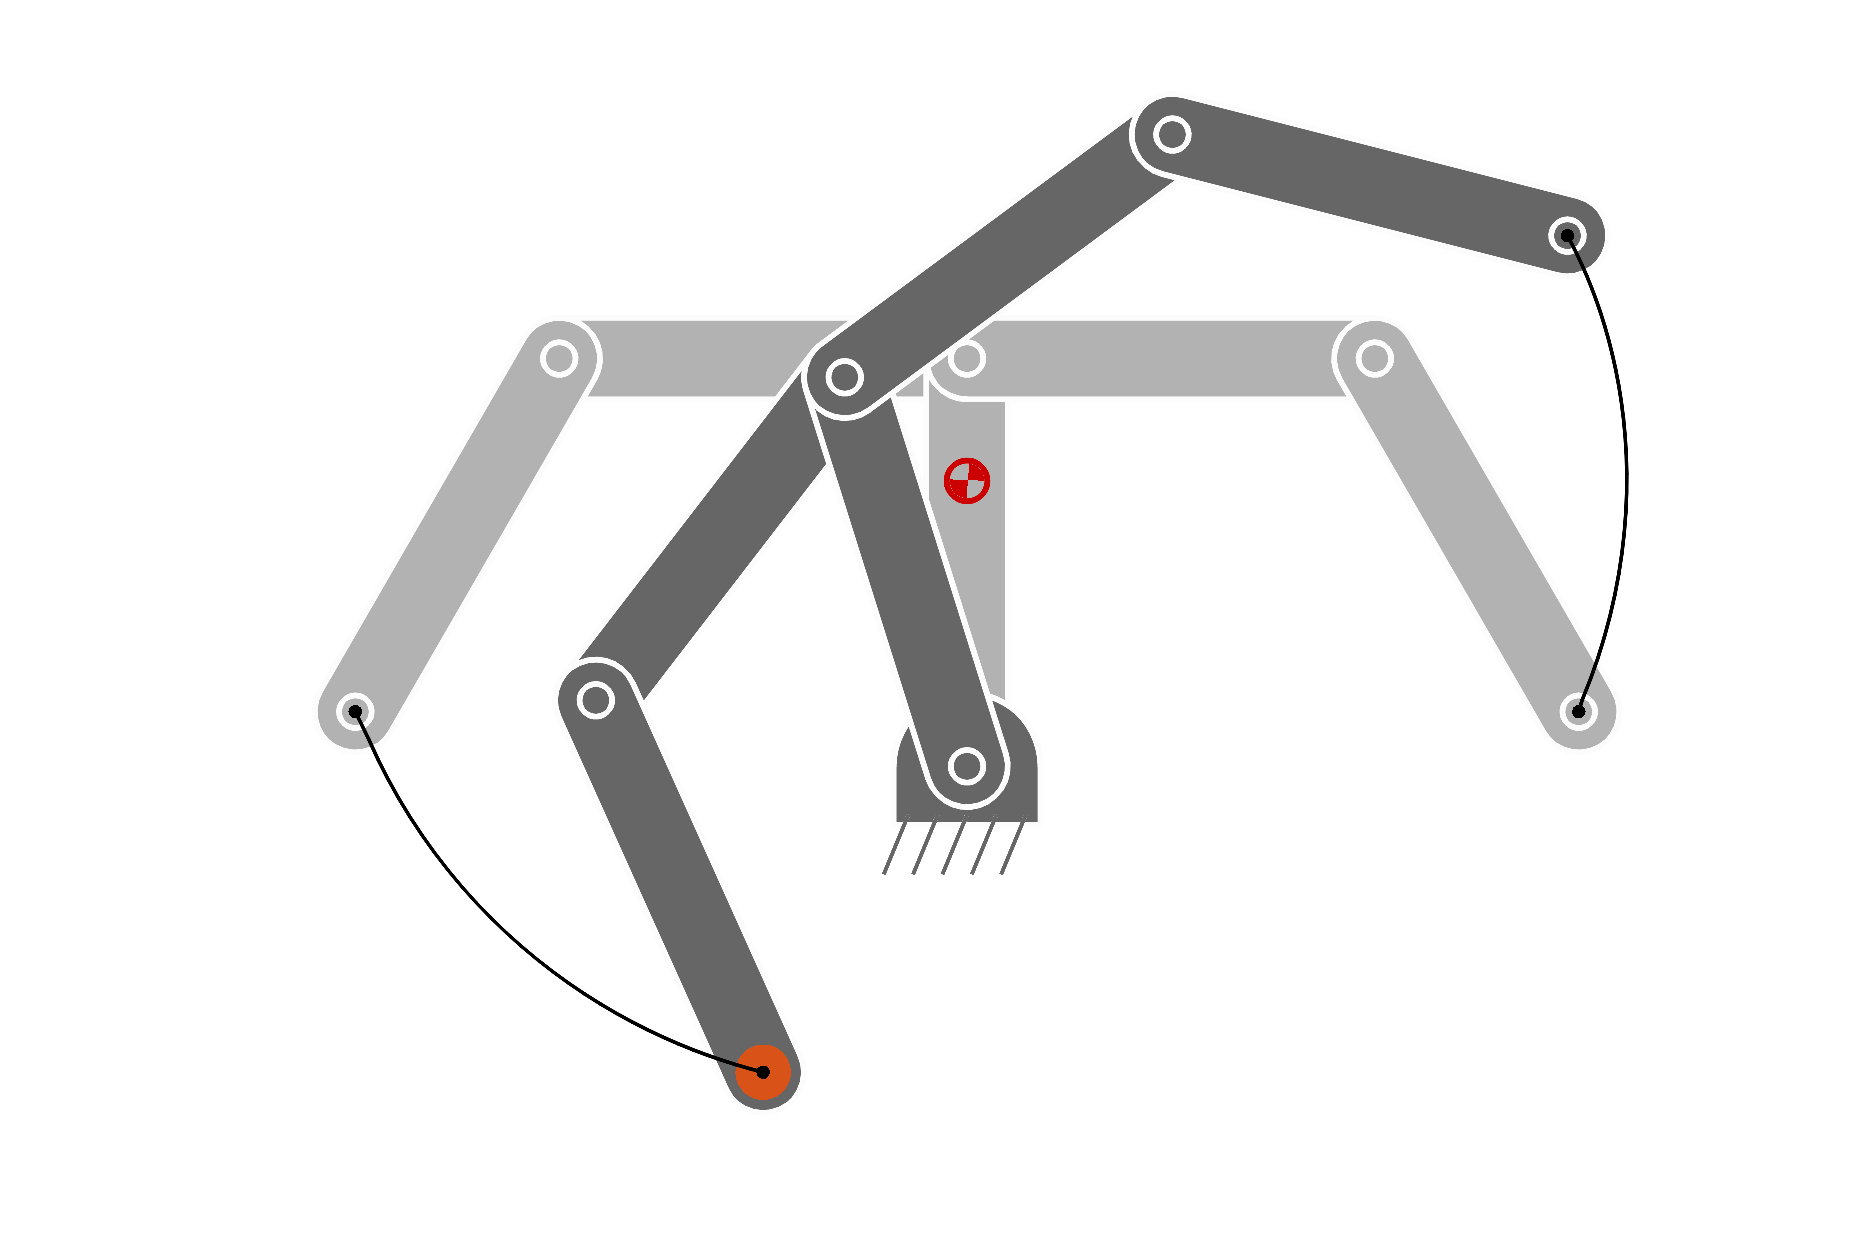
\includegraphics[width=.38\columnwidth]{images/iLQR_bimanual01.png}
\caption{\footnotesize
Reaching tasks with a bimanual robot (frontal view). \emph{Left:} with a target for each hand. \emph{Right:} with a target for the hand on the left, while keeping the center of mass at the same location during the whole movement.
}
\label{fig:iLQR_bimanual}
\end{SCfigure}

%\begin{wrapfigure}{r}{.36\textwidth}
%\vspace{-20pt}
%\centering
%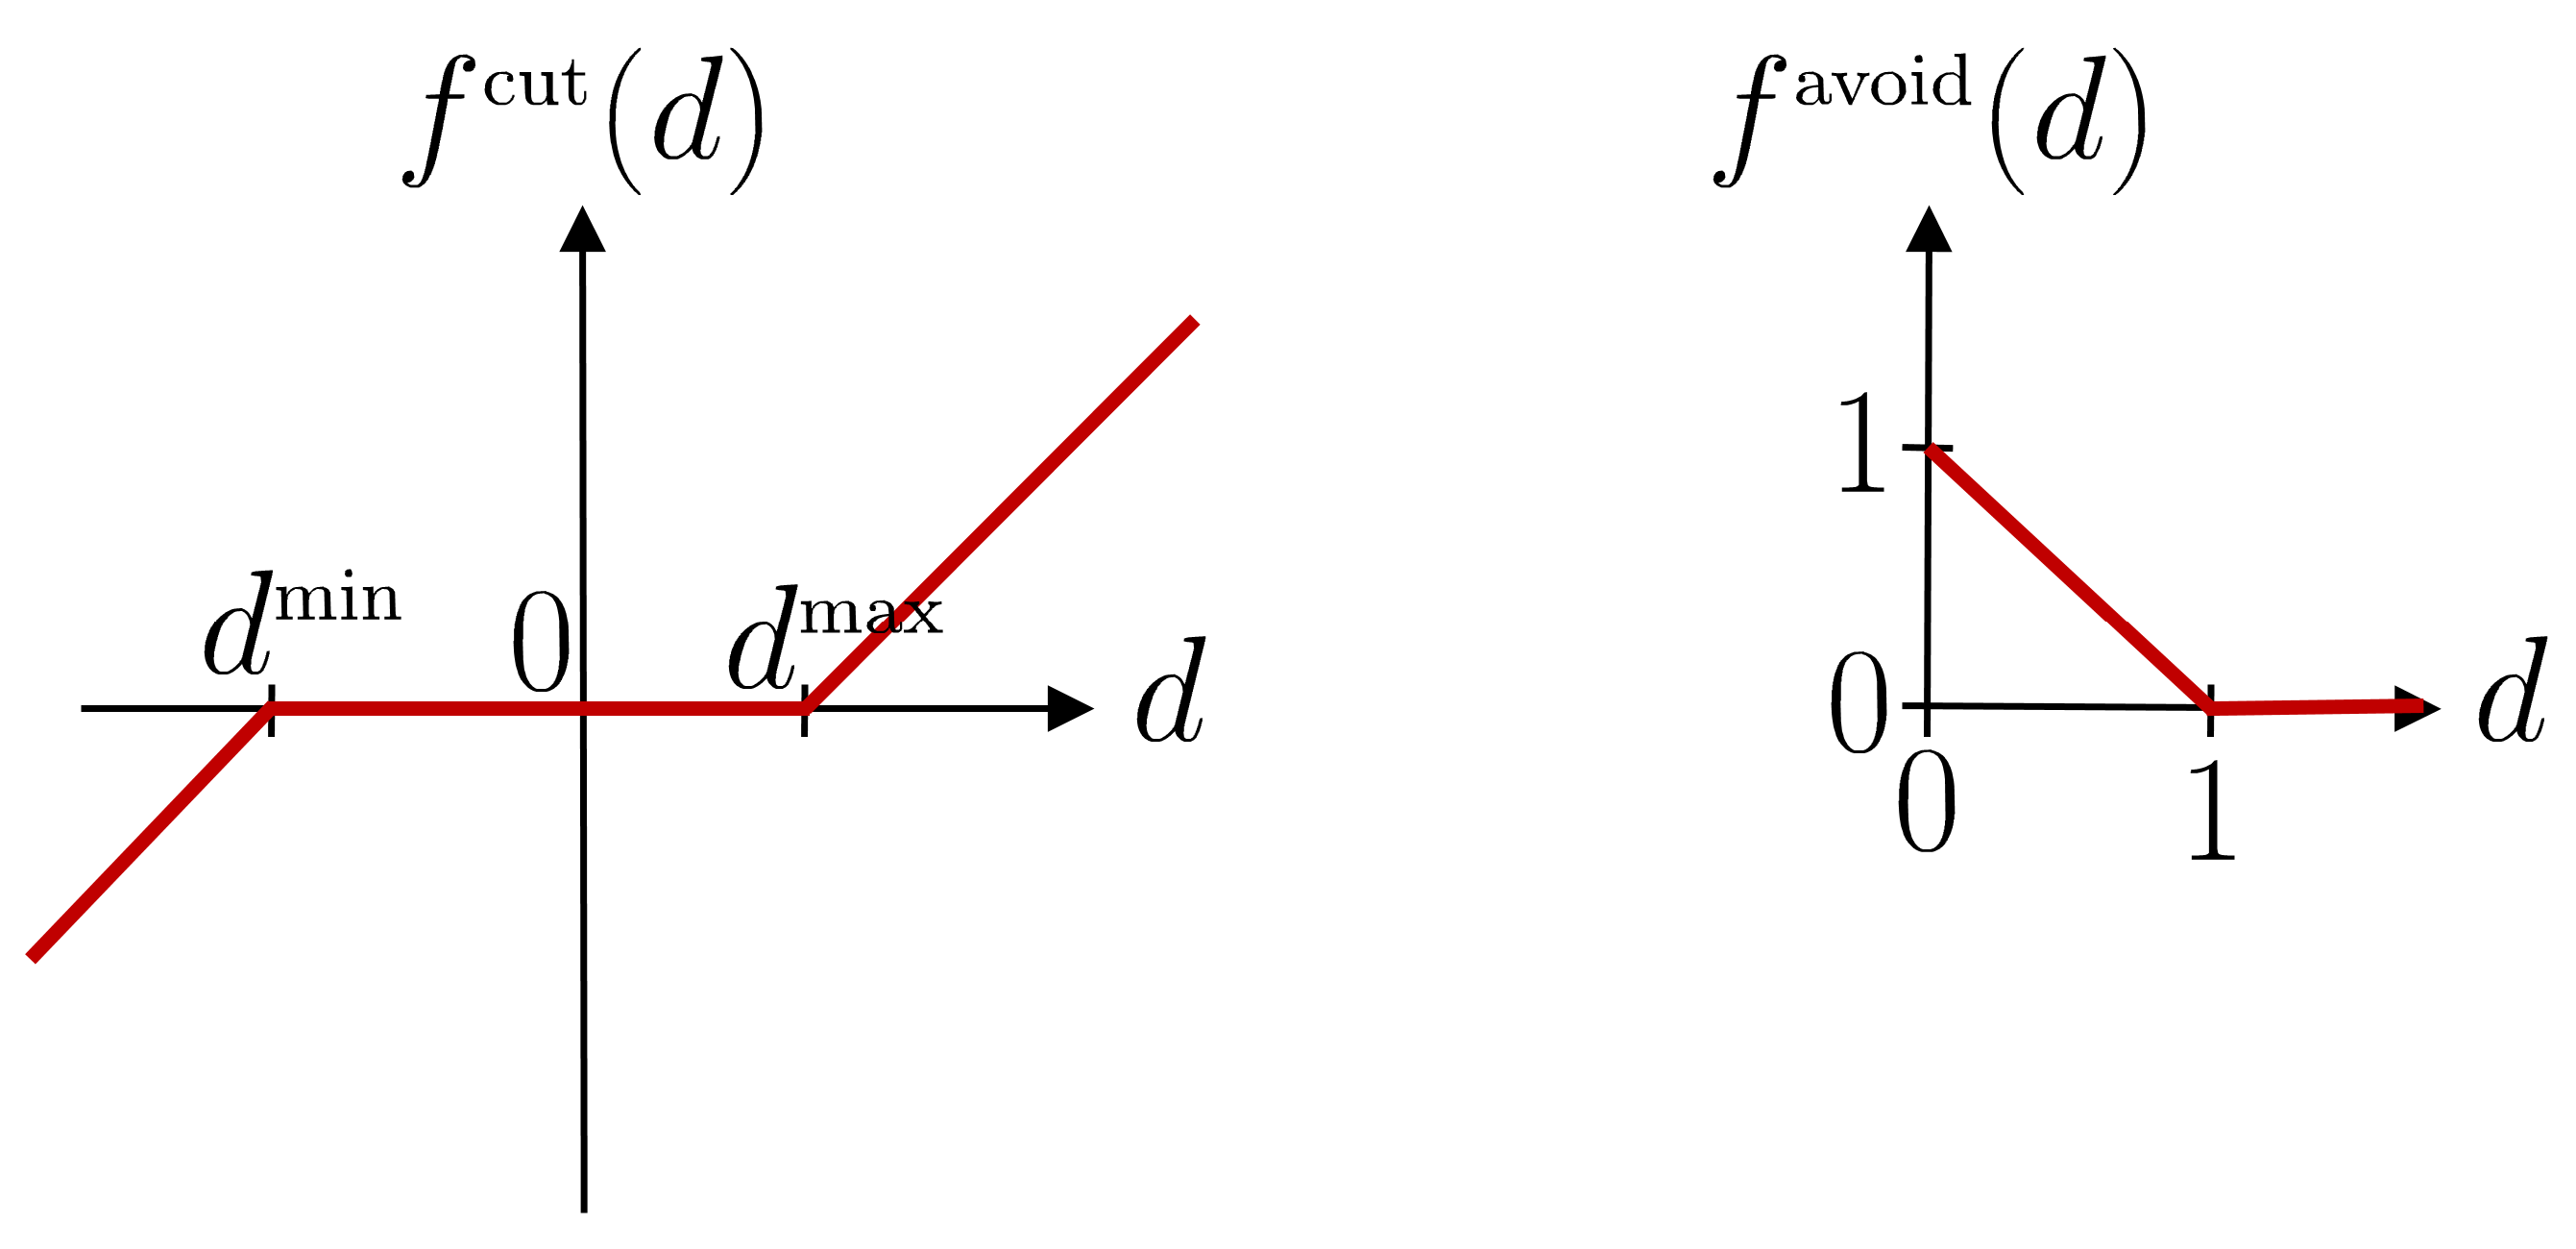
\includegraphics[width=.34\textwidth]{images/fcut01.png}
%\caption{\footnotesize
%Reaching tasks with a bimanual robot (frontal view). \emph{Left:} with a target for each hand. \emph{Right:} with a target for the hand on the left, while keeping the center of mass at the same location during the whole movement.
%}
%\label{fig:iLQR_bimanual}
%\vspace{-20pt}
%\end{wrapfigure}

We consider a 5-link planar bimanual robot with a torso link shared by the two arms, see Fig.~\ref{fig:iLQR_bimanual}. We define the forward kinematics function as
\begin{equation*}
	\bm{f} = \begin{bmatrix} 
	\bm{\ell}_\ty{[1,2,3]}^\trsp \cos(\bm{L}\bm{x}_\ty{[1,2,3]}) \\ 
	\bm{\ell}_\ty{[1,2,3]}^\trsp \sin(\bm{L}\bm{x}_\ty{[1,2,3]}) \\
	\bm{\ell}_\ty{[1,4,5]}^\trsp \cos(\bm{L}\bm{x}_\ty{[1,4,5]}) \\ 
	\bm{\ell}_\ty{[1,4,5]}^\trsp \sin(\bm{L}\bm{x}_\ty{[1,4,5]}) \\
	\end{bmatrix} \!\!,
\end{equation*}
%fee = [fkin(x(1:3,:), param.l(1:3)); fkin(x([1,4:5],:), param.l([1,4:5]))]
where the first two and last two dimensions of $\bm{f}$ correspond to the position of the left and right end-effectors, respectively. The corresponding Jacobian matrix $\bm{J}\in\mathbb{R}^{4\times 5}$ has entries
\begin{equation*}
	\bm{J}_\ty{[1,2],[1,2,3]} = \begin{bmatrix} 
	-\sin(\bm{L}\bm{x}_\ty{[1,2,3]})^\trsp \diag(\bm{\ell}_\ty{[1,2,3]}) \bm{L} \\ 
	 \cos(\bm{L}\bm{x}_\ty{[1,2,3]})^\trsp \diag(\bm{\ell}_\ty{[1,2,3]}) \bm{L} 
	\end{bmatrix},\quad
	\bm{J}_\ty{[3,4],[1,4,5]} = \begin{bmatrix} 
	-\sin(\bm{L}\bm{x}_\ty{[1,4,5]})^\trsp \diag(\bm{\ell}_\ty{[1,4,5]}) \bm{L} \\ 
	 \cos(\bm{L}\bm{x}_\ty{[1,4,5]})^\trsp \diag(\bm{\ell}_\ty{[1,4,5]}) \bm{L} 
	\end{bmatrix},\\
\end{equation*}
where the remaining entries are zeros.
%J = [-sin(L * x([1,2,3],t))' * diag(param.l([1,2,3])) * L; ...
%      cos(L * x([1,2,3],t))' * diag(param.l([1,2,3])) * L];
%J(3:4,[1,4:5]) = [-sin(L * x([1,4,5],t))' * diag(param.l([1,4,5])) * L; ...
%                   cos(L * x([1,4,5],t))' * diag(param.l([1,4,5])) * L];		                    

If we assume a unit mass for each arm link concentrated at the joint and a mass of two units at the tip of the first link (i.e., assuming that the motors and gripper are heavier than the link structures, and that two motors are located at the tip of the first link to control the left and right arms), the forward kinematics function to determine the center of a mass of the bimanual articulated chain in Fig.~\ref{fig:iLQR_bimanual} can be computed with
\begin{equation*}
	\bm{f}^\tp{CoM} = \frac{1}{6}\begin{bmatrix} 
	\bm{\ell}_\ty{[1,2,3]}^\trsp \bm{L} \cos(\bm{L}\bm{x}_\ty{[1,2,3]}) + 
	\bm{\ell}_\ty{[1,4,5]}^\trsp \bm{L} \cos(\bm{L}\bm{x}_\ty{[1,4,5]}) \\ 
	\bm{\ell}_\ty{[1,2,3]}^\trsp \bm{L} \sin(\bm{L}\bm{x}_\ty{[1,2,3]}) +
	\bm{\ell}_\ty{[1,4,5]}^\trsp \bm{L} \sin(\bm{L}\bm{x}_\ty{[1,4,5]})
	\end{bmatrix},
\end{equation*}
%fc = [param.l(1:3)' * L * cos(L * x(1:3,:)) + param.l([1,4:5])' * L * cos(L * x([1,4:5],:)); ...
%      param.l(1:3)' * L * sin(L * x(1:3,:)) + param.l([1,4:5])' * L * sin(L * x([1,4:5],:))] / 6;	      
with the corresponding Jacobian matrix $\bm{J}^\tp{CoM}\in\mathbb{R}^{2\times 5}$ computed as
\begin{equation*}
	\bm{J}^\tp{CoM} = \begin{bmatrix} 
	\bm{J}^\tp{CoM-L}_{[1,2],1} + \bm{J}^\tp{CoM-R}_{[1,2],1}, & \bm{J}^\tp{CoM-L}_{[1,2],[2,3]}, & \bm{J}^\tp{CoM-R}_{[1,2],[2,3]}
	\end{bmatrix},
\end{equation*}
\begin{equation*}	
	\text{with}\quad 
	\bm{J}^\tp{CoM-L} = \frac{1}{6}\begin{bmatrix} 
	-\sin(\bm{L}\bm{x}_\ty{[1,2,3]})^\trsp \bm{L} \; \diag(\bm{\ell}_\ty{[1,2,3]}^\trsp \bm{L}) \\ 
	\cos(\bm{L}\bm{x}_\ty{[1,2,3]})^\trsp \bm{L} \; \diag(\bm{\ell}_\ty{[1,2,3]}^\trsp \bm{L})
	\end{bmatrix},\quad
	\bm{J}^\tp{CoM-R} = \frac{1}{6}\begin{bmatrix} 
	-\sin(\bm{L}\bm{x}_\ty{[1,4,5]})^\trsp \bm{L} \; \diag(\bm{\ell}_\ty{[1,4,5]}^\trsp \bm{L}) \\ 
	\cos(\bm{L}\bm{x}_\ty{[1,4,5]})^\trsp \bm{L} \; \diag(\bm{\ell}_\ty{[1,4,5]}^\trsp \bm{L})
	\end{bmatrix}.
\end{equation*}
%J0l = [-sin(L * x(1:3,t))' * L * diag(param.l(1:3)' * L); ...
%        cos(L * x(1:3,t))' * L * diag(param.l(1:3)' * L)] / 6;
%J0r = [-sin(L * x([1,4:5],t))' * L * diag(param.l([1,4:5])' * L); ...
%        cos(L * x([1,4:5],t))' * L * diag(param.l([1,4:5])' * L)] / 6;
%J0 = [(J0l(:,1) + J0r(:,1)), J0l(:,2:end), J0r(:,2:end)];


%%%%%%%%%%%%%%%%%%%%%%%%%%%%%%%%%%%%%%%%%%%%%%%%%%%%%%%%%%%%%%%%%%%%%%%%%%%%%%%%%
\subsubsection{Obstacle avoidance with ellipsoid shapes} %(1-e'*e)'*(1-e'*e) version, where 1-e'*e is a scalar
\begin{flushright}
\filename{iLQR\_obstacle.*}
\end{flushright}

%\begin{figure}
%\centering
%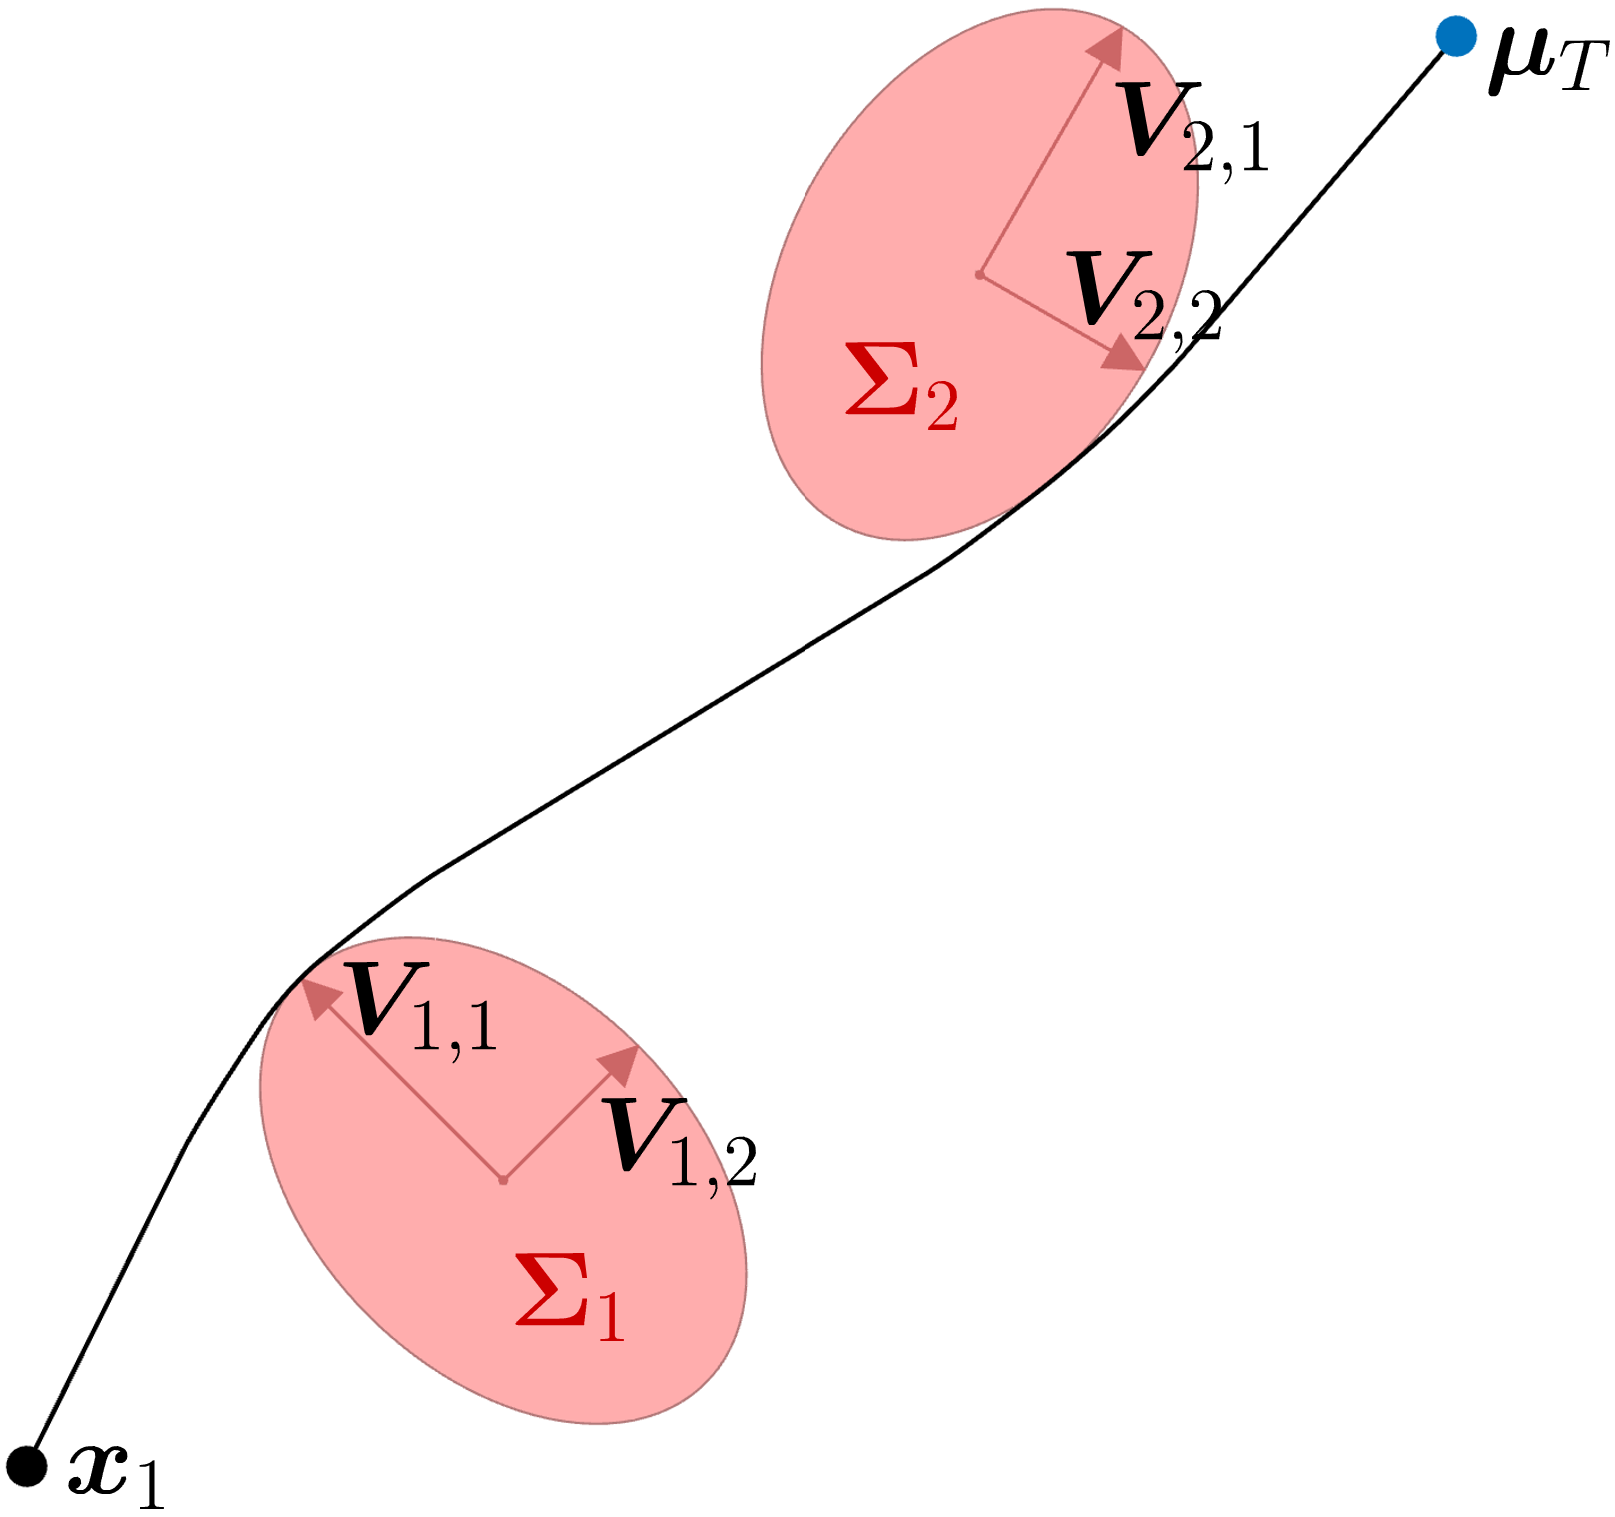
\includegraphics[width=.5\columnwidth]{images/iLQR_ellipsoidObstacle01.png}
%\caption{\footnotesize
%Reaching task with obstacle avoidance.
%}
%\label{fig:iLQR_obstacle}
%\end{figure}

\begin{wrapfigure}{r}{.32\textwidth}
%\vspace{-20pt}
\centering
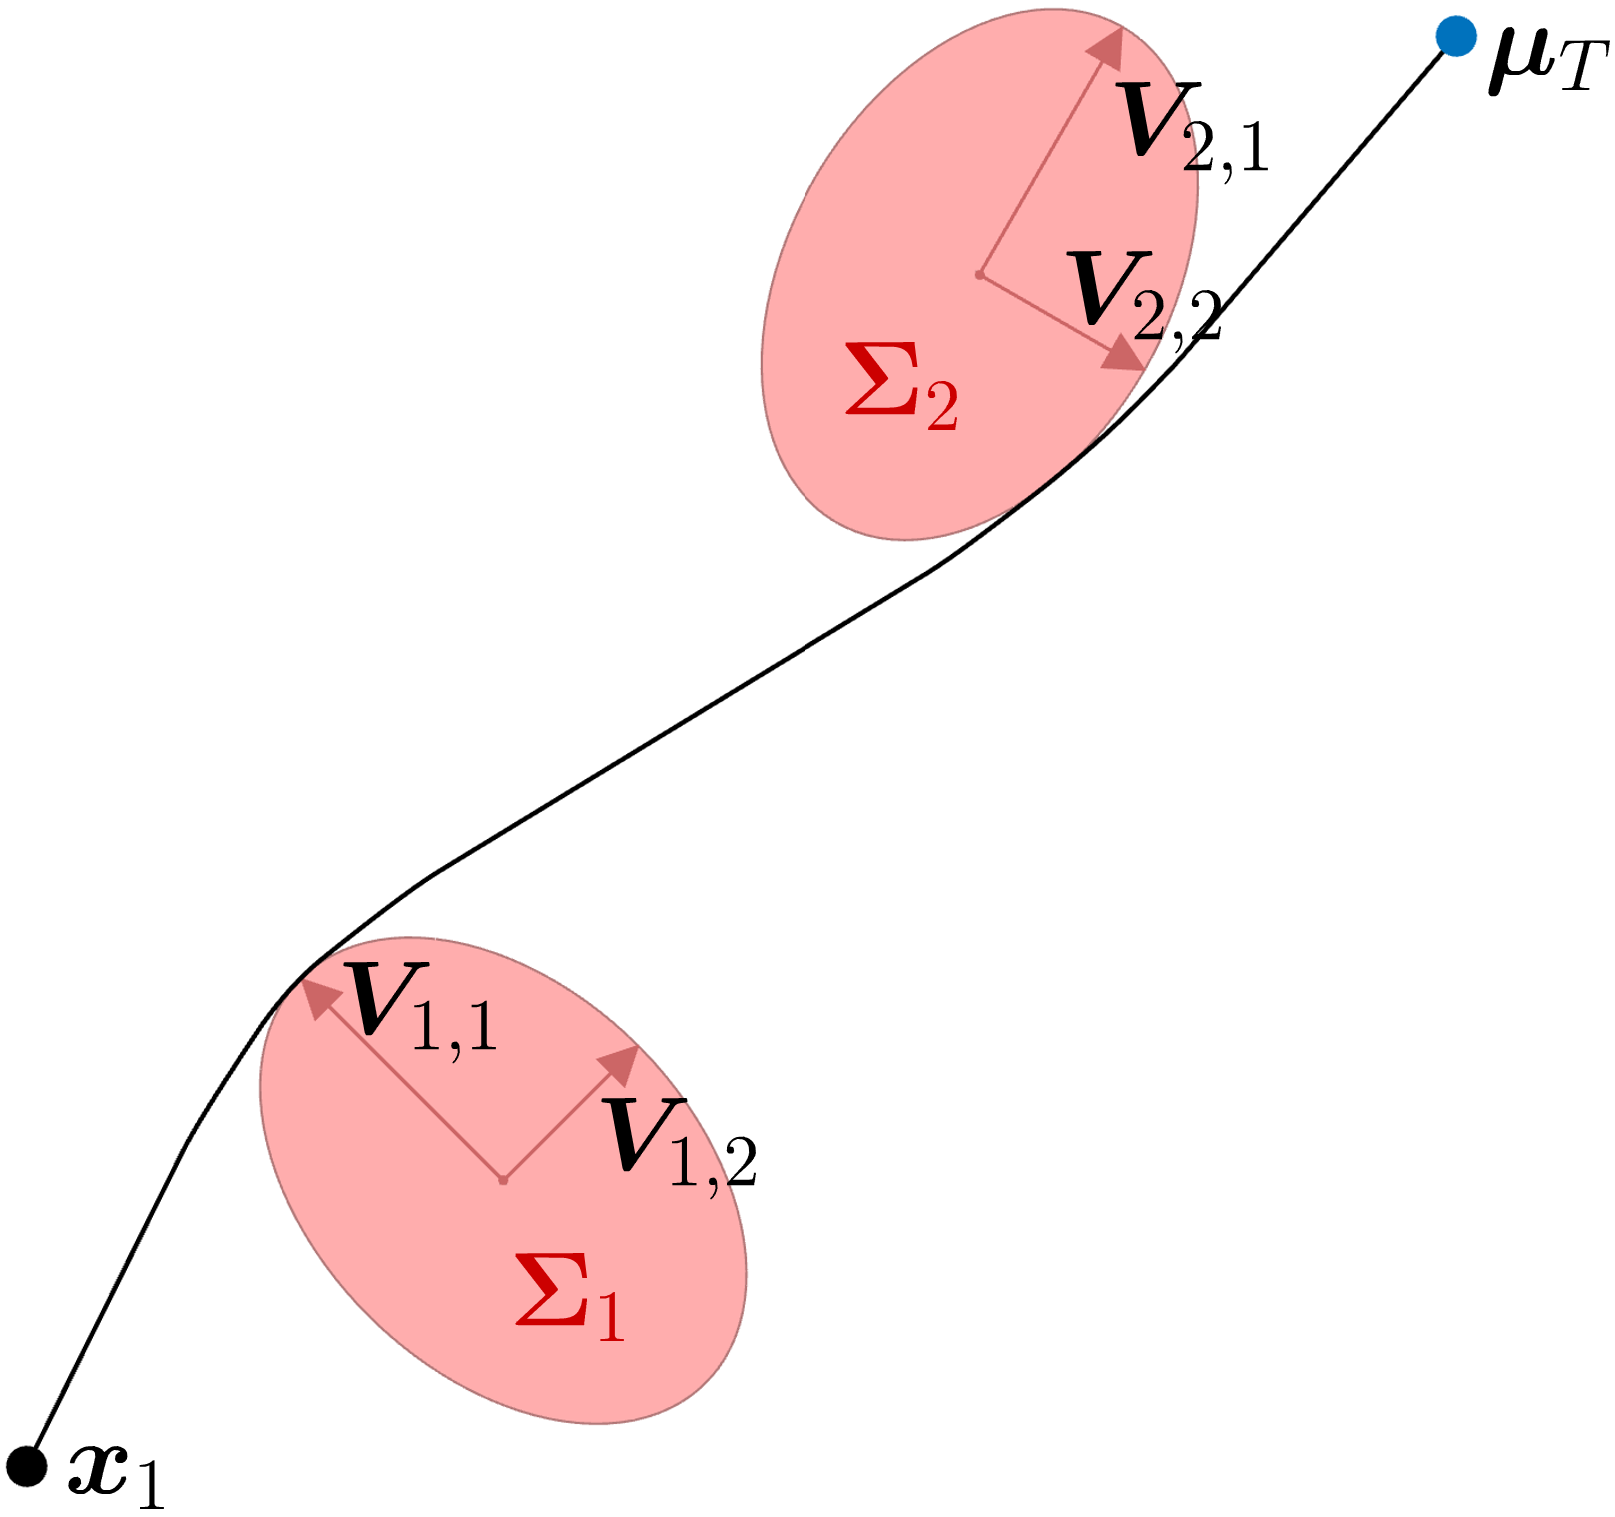
\includegraphics[width=.30\textwidth]{images/iLQR_ellipsoidObstacle01.png}
\caption{\footnotesize
Reaching task with obstacle avoidance, by starting from $\bm{x}_1$ and reaching $\bm{\mu}_T$ while avoiding the two obstacles in red.
}
\label{fig:iLQR_obstacle}
\vspace{-20pt}
\end{wrapfigure}

By taking as example a point-mass system, iLQR can be used to solve an ellipsoidal obstacle avoidance problem with the cost (typically used with other costs, see Fig.~\ref{fig:iLQR_obstacle} for an example). We first define a ReLU-like function and its gradient as (see also Fig.~\ref{fig:fcut}-\emph{right})
\begin{equation*} 
	f^\tp{avoid}(d) = \begin{cases} 0, & \text{if}\ d>1 \\ 1-d, & \text{otherwise} \end{cases}, \quad\quad
	g^\tp{avoid}(d) = \begin{cases} 0, \hspace{6mm} & \text{if}\ d>1 \\ -1, & \text{otherwise} \end{cases}, 
\end{equation*}
that we exploit to define $\bm{f}(\bm{x}_t)$ and $\bm{J}(\bm{x}_t)$ in \eqref{eq:du} as
\begin{align*}
	\bm{f}(\bm{x}_t) &= f^\tp{avoid}\Big( e(\bm{x}_t) \Big), \quad\quad
	\bm{J}(\bm{x}_t) = 2 \; g^\tp{avoid}\Big( e(\bm{x}_t) \Big) \; {(\bm{x}_t-\bm{\mu})}^\trsp \; \bm{\Sigma}^{-1} ,\\
	\text{with}\quad e(\bm{x}_t) &= {(\bm{x}_t-\bm{\mu})}^\trsp \bm{\Sigma}^{-1} (\bm{x}_t-\bm{\mu}).
\end{align*}

In the above, $\bm{f}(\bm{x})$ defines a continuous function that is $0$ outside the obstacle boundaries and $1$ at the center of the obstacle. The ellipsoid is defined by a center $\bm{\mu}$ and a shape $\bm{\Sigma}=\bm{V}\bm{V}^\trsp$, where $\bm{V}$ is a horizontal concatenation of vectors $\bm{V}_i$ describing the principal axes of the ellipsoid, see Fig.~\ref{fig:iLQR_obstacle}. 
%A similar decomposition on the corresponding precision matrix is expressed as $\bm{\Sigma}^{-1}=\bm{U}\bm{U}^\trsp$. 

A similar principle can be applied to robot manipulators by composing forward kinematics and obstacle avoidance functions.  

% By considering e(x) = U'*(mu-x) with Sigma=U*U', and f(x) = f^cut(e(x)'*e(x)) a ReLU-like function, we can define an avoidance cost in the form 
% c = f' * Q * f, which is a correct Gauss--Newton assumption.
%
% Alternatively, an avoidance cost c = (1 - f'*f) * wQ (with wQ a scalar weigh) can be used in practice because 0<=(1 - f'*f)<=1


%%%%%%%%%%%%%%%%%%%%%%%%%%%%%%%%%%%%%%%%%%%%%%%%%%%%%%%%%%%%%%%%%%%%%%%%%%%%%%%%%
\subsubsection{Maintaining a desired distance to an object} %(1-e'*e)'*(1-e'*e) version, where 1-e'*e is a scalar
\begin{flushright}
\filename{iLQR\_distMaintenance.*}
\end{flushright}

The obstacle example above can easily be extended to the problem of maintaining a desired distance to an object, which can also typically used with other objectives. We first define a function and a gradient
\begin{equation*} 
	f^\tp{dist}(d) = 1-d, \quad\quad
	g^\tp{dist}(d) = -1,
\end{equation*}
that we exploit to define $\bm{f}(\bm{x}_t)$ and $\bm{J}(\bm{x}_t)$ in \eqref{eq:du} as
\begin{align*}
	\bm{f}(\bm{x}_t) &= f^\tp{dist}\Big( e(\bm{x}_t) \Big), \quad\quad
	\bm{J}(\bm{x}_t) = -\frac{2}{r^2} {(\bm{x}_t-\bm{\mu})}^\trsp ,\\ %\; g^\tp{dist}\Big( e(\bm{x}_t) \Big)
	\text{with}\quad e(\bm{x}_t) &= \frac{1}{r^2} {(\bm{x}_t-\bm{\mu})}^\trsp (\bm{x}_t-\bm{\mu}).
\end{align*}

In the above, $\bm{f}(\bm{x})$ defines a continuous function that is $0$ on a sphere of radius $r$ centered on the object (defined by a center $\bm{\mu}$), and increasing/decreasing when moving away from this surface in one direction or the other. 


%%%%%%%%%%%%%%%%%%%%%%%%%%%%%%%%%%%%%%%%%%%%%%%%%%%%%%%%%%%%%%%%%%%%%%%%%%%%%%%%%
\subsubsection{Manipulability tracking}
\begin{flushright}
\filename{iLQR\_bimanual\_manipulability.*}
\end{flushright}

\begin{SCfigure}[50]
\centering
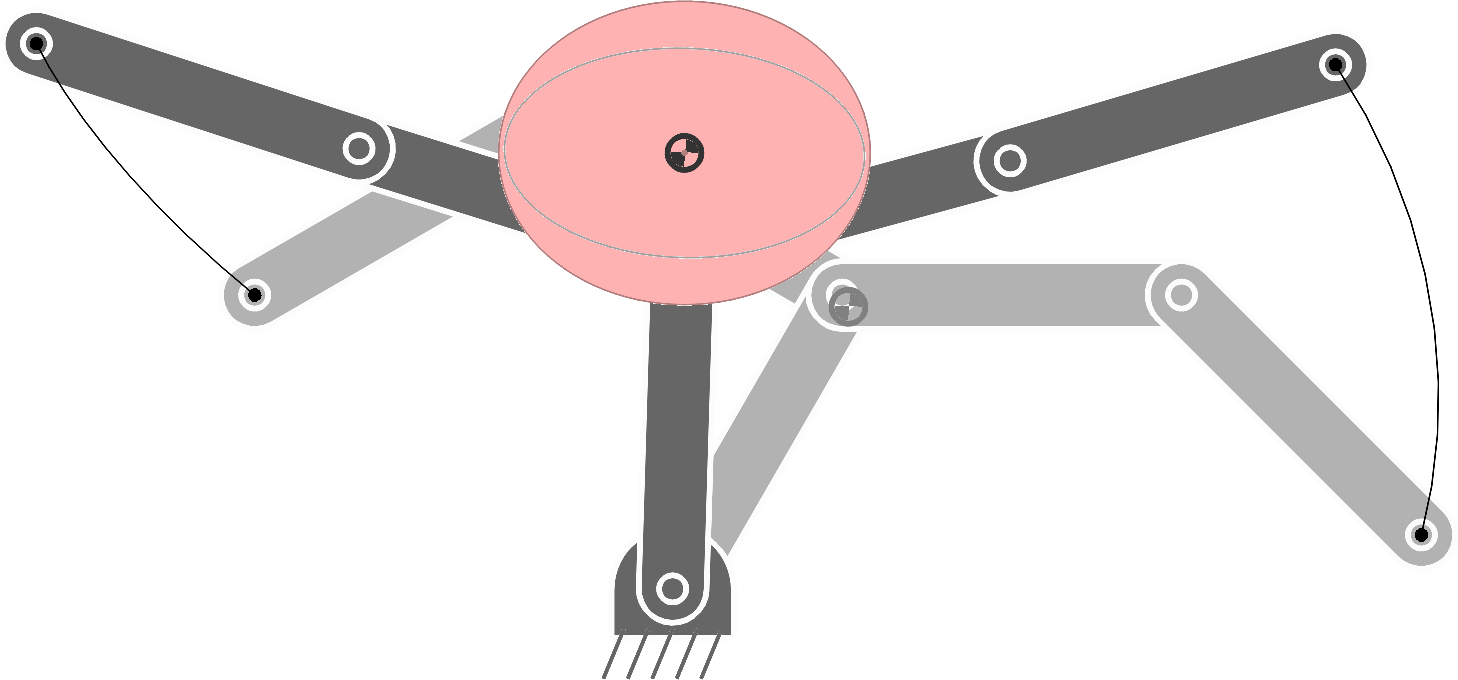
\includegraphics[width=.4\columnwidth]{images/iLQR_manipulability01.png}
\caption{\footnotesize
Example of iLQR optimization with a cost on manipulability, where the goal is to reach, at the end of the motion, a desired manipulability defined at the center of mass (CoM) of a bimanual planar robot. The initial pose of the bimanual robot is displayed in light gray and the final pose of the robot is displayed in dark gray. The desired manipulability is represented by the red ellipse. The achieved manipulability at the end of the motion is represented by the gray ellipse. Both manipulability ellipses are displayed at the CoM reached at the end of the motion, displayed as a semi-filled dark gray disc (the CoM at the beginning of the motion is displayed in lighter gray color). We can see that the posture adopted by the robot to approach the desired manipulability is to extend both arms, which is the pose allowing the robot to swiftly move its center of mass in case of unexpected perturbations.
}
\label{fig:iLQR_manipulability}
\end{SCfigure}

Skills transfer can exploit manipulability ellipsoids in the form of geometric descriptors representing the skills to be transferred to the robot. As these ellipsoids lie on symmetric positive definite (SPD) manifolds, Riemannian geometry can be used to learn and reproduce these descriptors in a probabilistic manner \cite{Calinon20RAM}.

Manipulability ellipsoids come in different flavors. They can be defined for either positions or forces (including the orientation/rotational part). Manipulability can be described at either kinematic or dynamic levels, for either open or closed linkages (e.g., for bimanual manipulation or in-hand manipulation), and for either actuated or non-actuated joints \cite{Park98}. This large set of manipulability ellipsoids provide rich descriptors to characterize robot skills for robots with legs and arms. 

Manipulability ellipsoids are helpful descriptors to handle skill transfer problems involving dissimilar kinematic chains, such as transferring manipulation skills between humans and robots, or between two robots with different kinematic chains or capabilities. In such transfer problems, imitation at joint angles level is not possible due to the different structures, and imitation at end-effector(s) level is limited, because it does not encapsulate postural information, which is often an essential aspect of the skill that we would like to transfer. Manipulability ellipsoids provide intermediate descriptors that allows postural information to be transferred indirectly, with the advantage that it allows different embodiments and capabilities to be considered in the skill transfer process.

The manipulability ellipsoid $\bm{M}(\bm{x}) = \bm{J}(\bm{x}) {\bm{J}(\bm{x})}^\trsp$ is a symmetric positive definite matrix representing the manipulability at a given point on the kinematic chain defined by a forward kinematics function $\bm{f}(\bm{x})$, given the joint angle posture $\bm{x}$, where $\bm{J}(\bm{x})$ is the Jacobian of $\bm{f}(\bm{x})$. The determinant of $\bm{M}(\bm{x})$ is often used as a scalar manipulability index indicating the volume of the ellipsoid \cite{Yoshikawa85}, with the drawback of ignoring the specific shape of this ellipsoid. 

In \cite{Jaquier21IJRR}, we showed that a geometric cost on manipulability can alternatively be defined with the geodesic distance
\begin{align}
	c &= \|\bm{A}\|^2_\text{F}, \quad\text{with}\quad \bm{A} = \log\!\big( \bm{S}^\frac{1}{2} \bm{M}(\bm{x}) \bm{S}^\frac{1}{2} \big), \nonumber\\
	\iff\; 
	c &= \text{trace}(\bm{A}\bm{A}^\trsp)=\sum_i\text{trace}(\bm{A}_i\bm{A}_i^\trsp) = \sum_i\bm{A}_i^\trsp\bm{A}_i 
	= {\text{vec}(\bm{A})}^\trsp \text{vec}(\bm{A}),
	\label{eq:cManipulability}
\end{align}
where $\bm{S}$ is the desired manipulability matrix to reach, $\log(\cdot)$ is the logarithm matrix function, and $\| \cdot \|_\text{F}$ is a Frobenius norm. By exploiting the trace properties, we can see that \eqref{eq:cManipulability} can be expressed in a quadratic form, where the vectorization operation $\text{vec}(\bm{A})$ can be computed efficiently by exploiting the symmetry of the matrix $\bm{A}$. This is implemented by keeping only the lower half of the matrix, with the elements below the diagonal multiplied by a factor $\sqrt{2}$.
%A=rand(3,2)-.5; trace(A*A') = trace(A'*A) = A(:,1)'*A(:,1)+A(:,2)'*A(:,2) = A(:)'*A(:)

The derivatives of \eqref{eq:cManipulability} with respect to the state $\bm{x}$ and control commands $\bm{u}$ can be computed numerically (as in the provided example), analytically (by following an approach similar to the one presented in \cite{Jaquier21IJRR}), or by automatic differentiation. The quadratic form of \eqref{eq:cManipulability} can be exploited to solve the problem with Gauss--Newton optimization, by using Jacobians (see description in Section \ref{sec:IKnum} within the context of inverse kinematics). Mari\'c \emph{et al.} demonstrated the advantages of a geometric cost as in \eqref{eq:cManipulability} for planning problems, by comparing it to alternative widely used metrics such as the manipulability index and the dexterity index \cite{Maric21}.

Note here that manipulability can be defined at several points of interest, including endeffectors and centers of mass. Figure \ref{fig:iLQR_manipulability} presents a simple example with a bimanual robot. Manipulability ellipsoids can also be exploited as descriptors for object affordances, by defining manipulability at the level of specific points on objects or tools held by the robot. For example, we can consider a manipulability ellipsoid at the level of the head of a hammer. When the robot grasps the hammer, its endeffector is extended so that the head of the hammer becomes the extremity of the kinematic chain. In this situation, the different options that the robot has to grasp the hammer will have an impact on the resulting manipulability at the head of the hammer. Thus, grabbing the hammer at the extremity of the handle will improve the resulting manipulability. Such descriptors offer promises for learning and optimization in manufacturing environments, in order to let robots automatically determine the correct ways to employ tools, including grasping points and body postures. 

The above iLQR approach, with a geodesic cost on SPD manifolds, has been presented for manipulability ellipsoids, but it can be extended to other descriptors represented as ellipsoids. In particular, stiffness, feedback gains, inertia, and centroidal momentum have similar structures. For the latter, the centroidal momentum ellipsoid quantifies the momentum generation ability of the robot \cite{Orin08}, which is another useful descriptor for robotics skills. Similarly to manipulability ellipsoids, it is constructed from Jacobians, which are in this case the centroidal momentum matrices mapping the joint angle velocities to the centroidal momentum, which sums over the individual link momenta after projecting each to the robot's center of mass.

The approach can also be extended to other forms of symmetric positive definite matrices, such as kernel matrices used in machine learning algorithms to compute similarities, or graph graph Laplacians (a matrix representation of a graph that can for example be used to construct a low dimensional embedding of a graph).

%%%%%%%%%%%%%%%%%%%%%%%%%%%%%%%%%%%%%%%%%%%%%%%%%%%%%%%%%%%%%%%%%%%%%%%%%%%%%%%%%
\subsubsection{Decoupling of control commands}

\begin{wrapfigure}{r}{.22\textwidth}
%\vspace{-20pt}
\centering
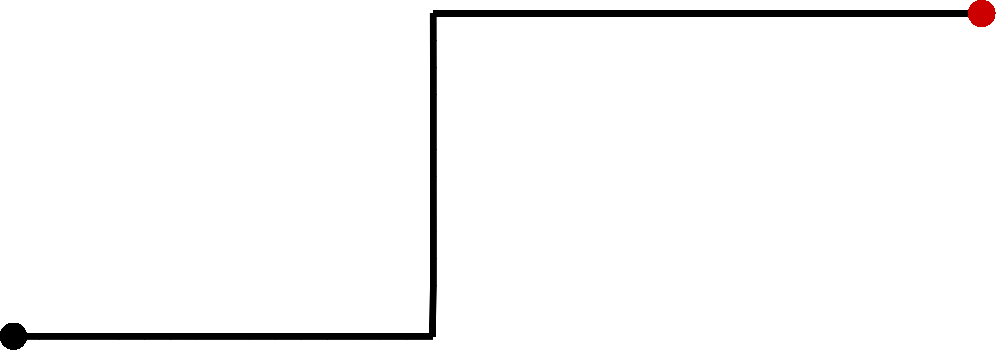
\includegraphics[width=.20\textwidth]{images/iLQR_decoupling01.png}
\caption{\footnotesize
2D reaching task problem (initial point in black and target point in red), with an additional cost to favor the decoupling of the control commands.
}
\label{fig:iLQR_decoupling}
\end{wrapfigure}

In some situations, we would like to control a robot by avoiding that all degrees of freedom are controlled at the same time. For example, we might in some cases  prefer that a mobile manipulator stops moving the arm while the platform is moving and vice versa.

For a 2 DOFs robot controlled at each time step $t$ with two control command $u_{1,t}$ and $u_{2,t}$, the corresponding cost to find the full sequence of control commands for a duration $T$ (gathered in a concatenated vector $\bm{u}$) is
\begin{equation*}
	\min_{\bm{u}} \; \sum_{t=1}^T \, {(u_{1,t} \, u_{2,t})}^2,
\end{equation*}
with corresponding residuals and Jacobian given by 
\begin{equation*}
	r_t = u_{1,t} \, u_{2,t},
	\quad
	\bm{J}_t = \big[ u_{2,t}, \, u_{1,t} \big], 
	\quad 
	\forall t\in\{1,\ldots,T\}.
\end{equation*}

The Gauss--Newton update rule in concatenated vector form is given by
\begin{equation*}
	\bm{u}_{k+1} \;\leftarrow\; 
	\bm{u}_k - \alpha \, {\big( \bm{J}^\trsp \bm{J} \big)}^{\!-1} \, \bm{J}^\trsp \, \bm{r},
\end{equation*}
where $\alpha$ is a line search parameter, $\bm{r}$ is a vector concatenating vertically all residuals $r_t$, and $\bm{J}$ is a Jacobian matrix with $\bm{J}_t$ as block diagonal elements. With some linear algebra machinery, this can also be computed in batch form using $\bm{r} = \bm{u}_1 \odot \bm{u}_2$, and $\bm{J} = (\bm{I}_{T-1} \otimes \bm{1}_{1\times 2}) \; \text{diag}\Big(\big(\bm{I}_{T-1} \otimes (\bm{1}_{2\times 2}-\bm{I}_2)\big)\bm{u} \Big)$, with $\odot$ and $\otimes$ the elementwise product and Kronecker product operators, respectively. 

Figure \ref{fig:iLQR_decoupling} presents a simple example within a 2D reaching problem with a point mass agent and velocity commands.

\newpage

%%%%%%%%%%%%%%%%%%%%%%%%%%%%%%%%%%%%%%%%%%%%%%%%%%%%%%%%%%%%%%%%%%%%%%%%%%%%%%%%%
\subsection{iLQR with control primitives}
\begin{flushright}
\filename{iLQR\_CP.*}
\end{flushright}

\begin{figure}
\centering
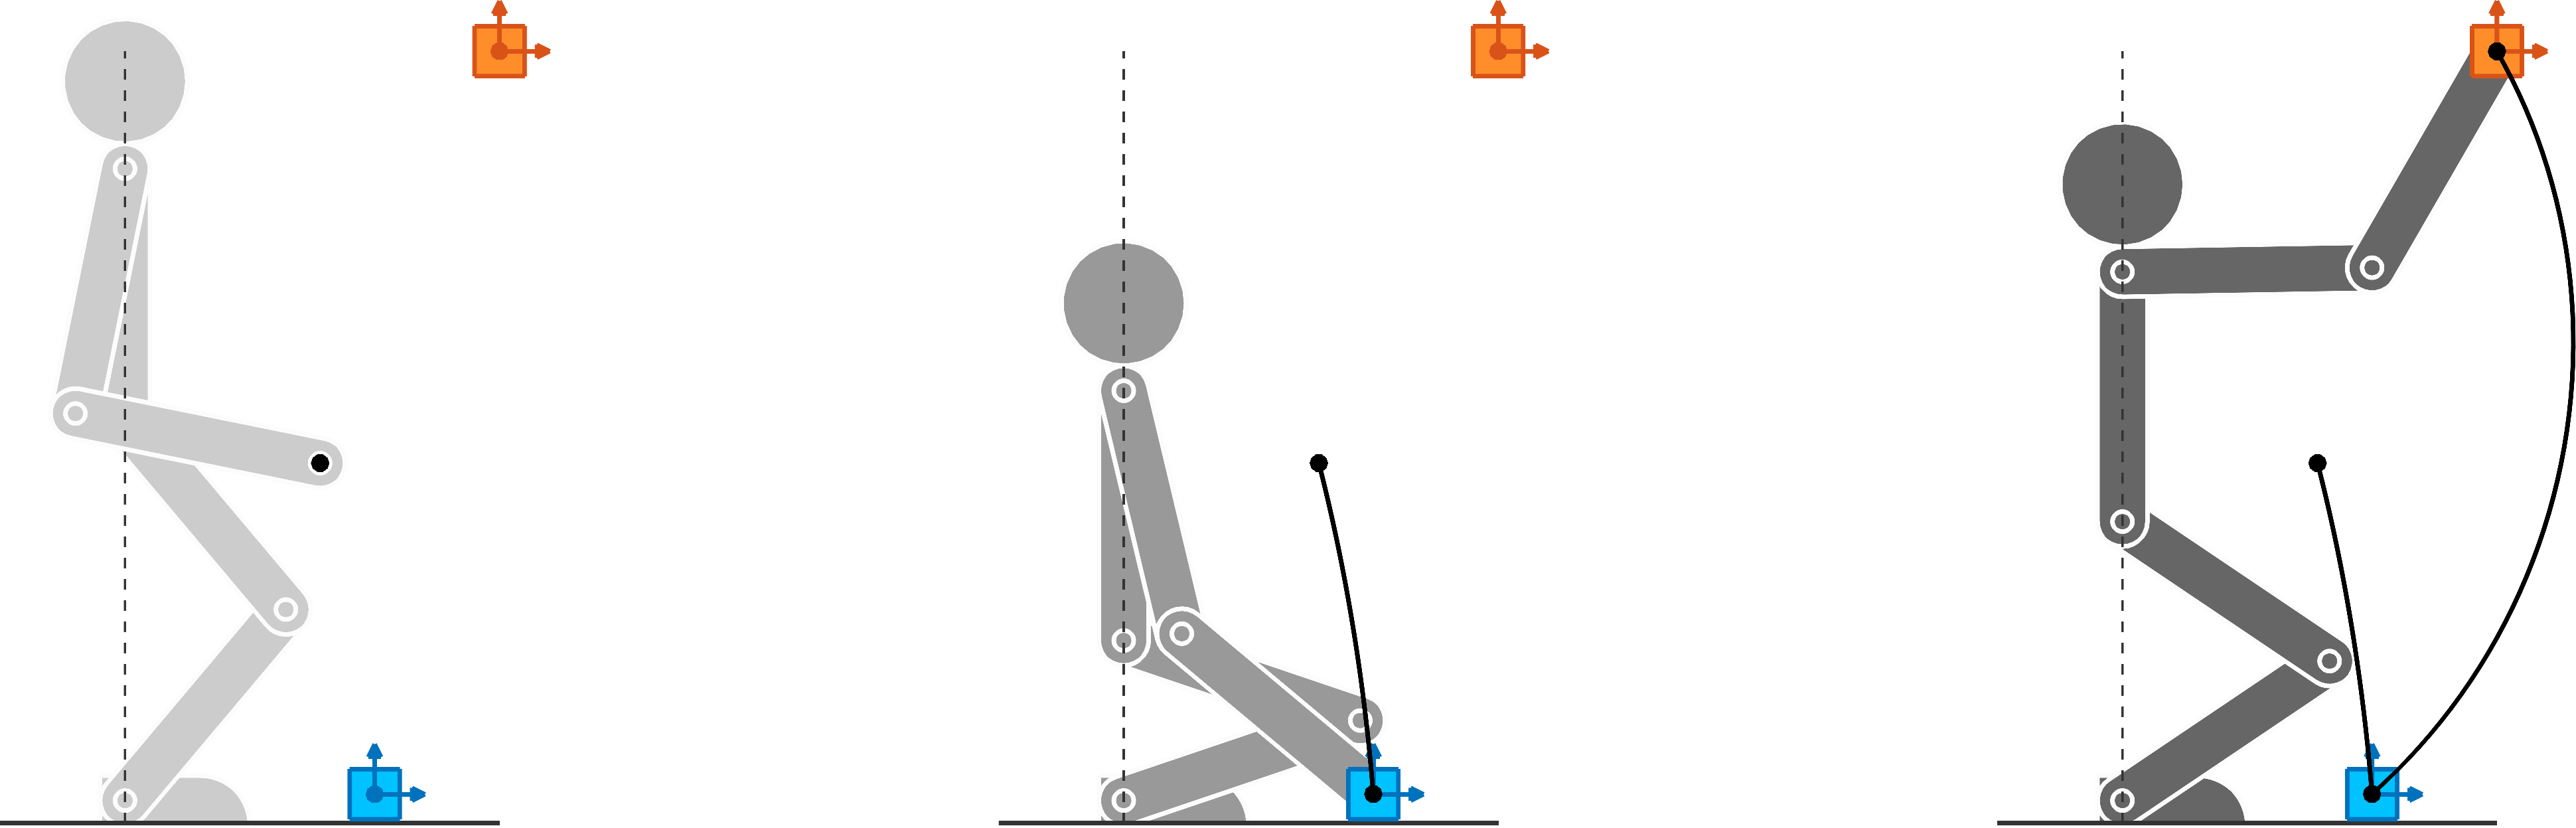
\includegraphics[width=.6\columnwidth]{images/iLQR_humanoid_CP01.png}
\caption{\footnotesize
Reaching task with control primitives.
}
\label{fig:iLQR_humanoid}
\end{figure}

The use of control primitives can be extended to iLQR, by considering $\Delta\bm{u}=\bm{\Psi}\Delta\bm{w}$. 
For problems with quadratic cost on $\bm{f}(\bm{x}_t)$ (see previous Section), the update of the weights vector is then given by
\begin{equation}
	\Delta\bm{\hat{w}} \!=\! {\Big( \bm{\Psi}^{\!\trsp}\bm{S}_{\bm{u}}^\trsp \bm{J}(\bm{x})^\trsp \bm{Q} \bm{J}(\bm{x}) \bm{S}_{\bm{u}} \bm{\Psi} 
	+ \bm{\Psi}^{\!\trsp} \bm{R}\, \bm{\Psi} \Big)}^{\!\!-1} 
	\Big(- \bm{\Psi}^{\!\trsp} \bm{S}_{\bm{u}}^\trsp \bm{J}(\bm{x})^\trsp \bm{Q} \bm{f}(\bm{x}) - \bm{\Psi}^{\!\trsp} \bm{R} \, \bm{u} \Big).
	\label{eq:dw}
\end{equation}

For a 5-link kinematic chain, by setting the coordination matrix in \eqref{eq:Psi2} as
\begin{equation*}
	\bm{C} = \begin{bmatrix}-1 & 0 & 0 \\ 2 & 0 & 0 \\ -1 & 0 & 0 \\ 0 & 1 & 0 \\ 0 & 0 & 1\end{bmatrix},
\end{equation*}
the first three joints are coordinated such that the third link is always oriented in the same direction, while the last two joints can move independently. Figure \ref{fig:iLQR_humanoid} shows an example for a reaching task, with the 5-link kinematic chain depicting a humanoid robot that needs to keep its torso upright.

Note also that the iLQR updates in \eqref{eq:dw} can usually be computed faster than in the original formulation, since a matrix of much smaller dimension needs to be inverted. 
%($DK\!\times\!DK$instead of $DT\!\times\!DT$)


%%%%%%%%%%%%%%%%%%%%%%%%%%%%%%%%%%%%%%%%%%%%%%%%%%%%%%%%%%%%%%%%%%%%%%%%%%%%%%%%%
\subsection{iLQR for spacetime optimization}

%\begin{figure}
%\centering
%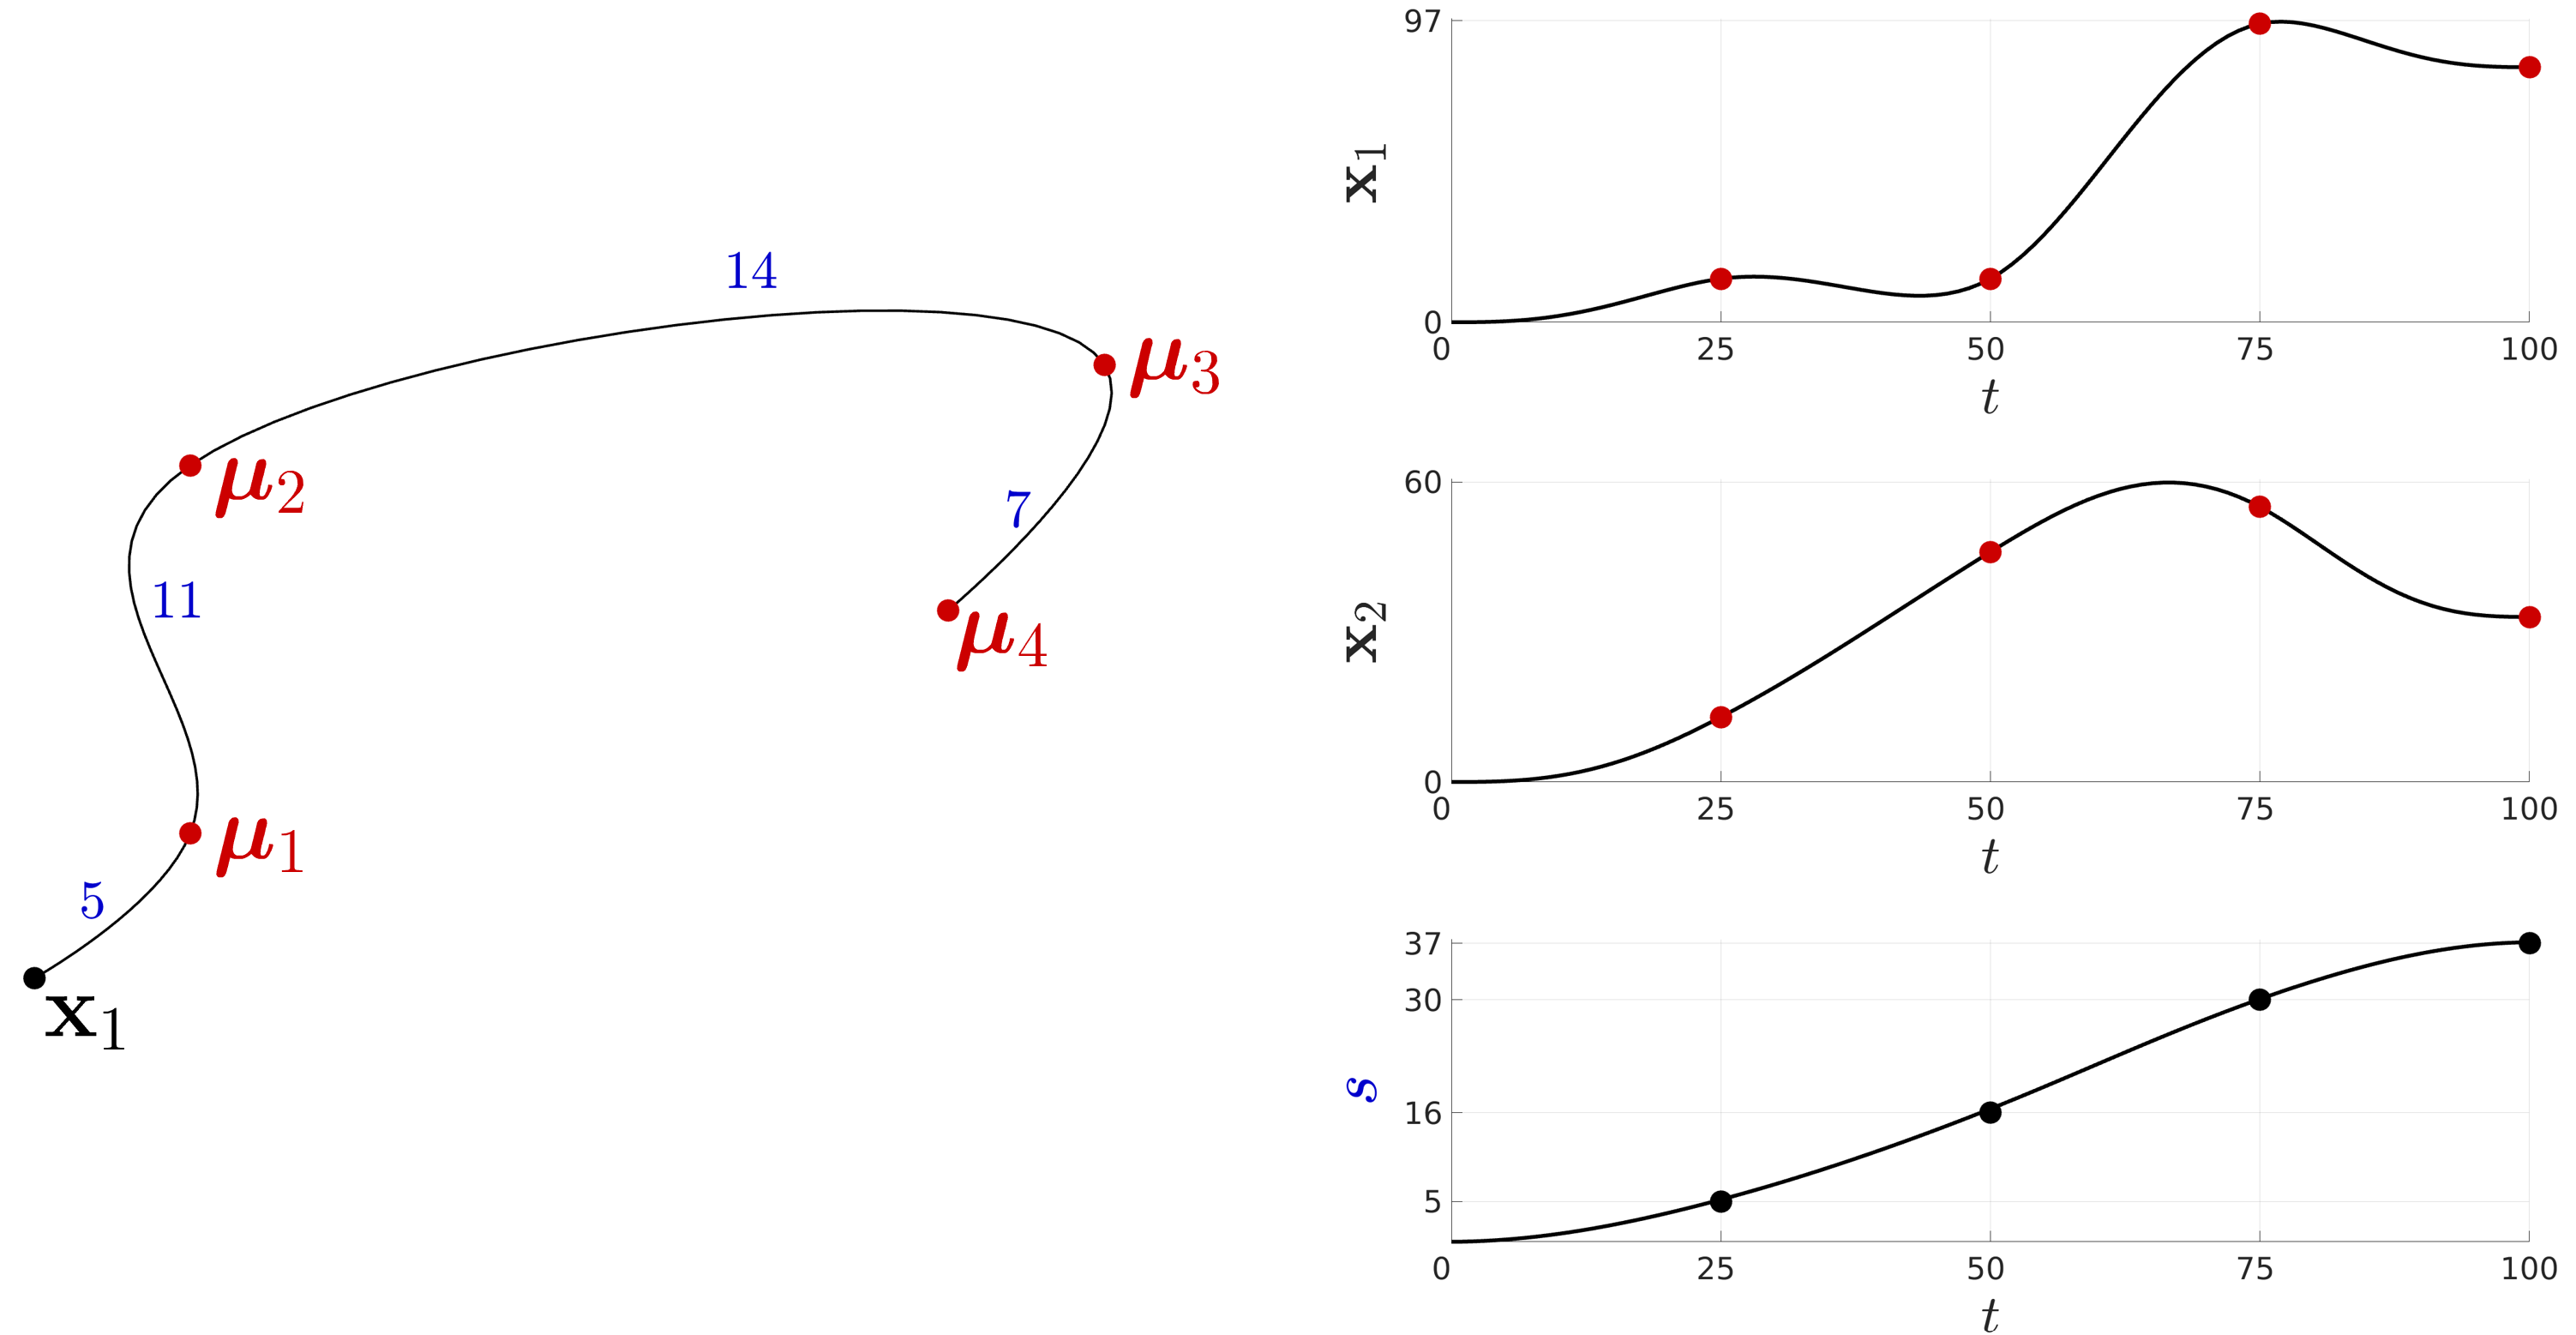
\includegraphics[width=\columnwidth]{images/iLQR_spacetime01.png}
%\caption{\footnotesize
%Spacetime optimization with iLQR for a viapoints task, where the estimated durations between consecutive viapoints are shown in blue. 
%}
%\label{fig:iLQR_spacetime}
%\end{figure}

\begin{wrapfigure}{r}{.52\textwidth}
%\vspace{-20pt}
\centering
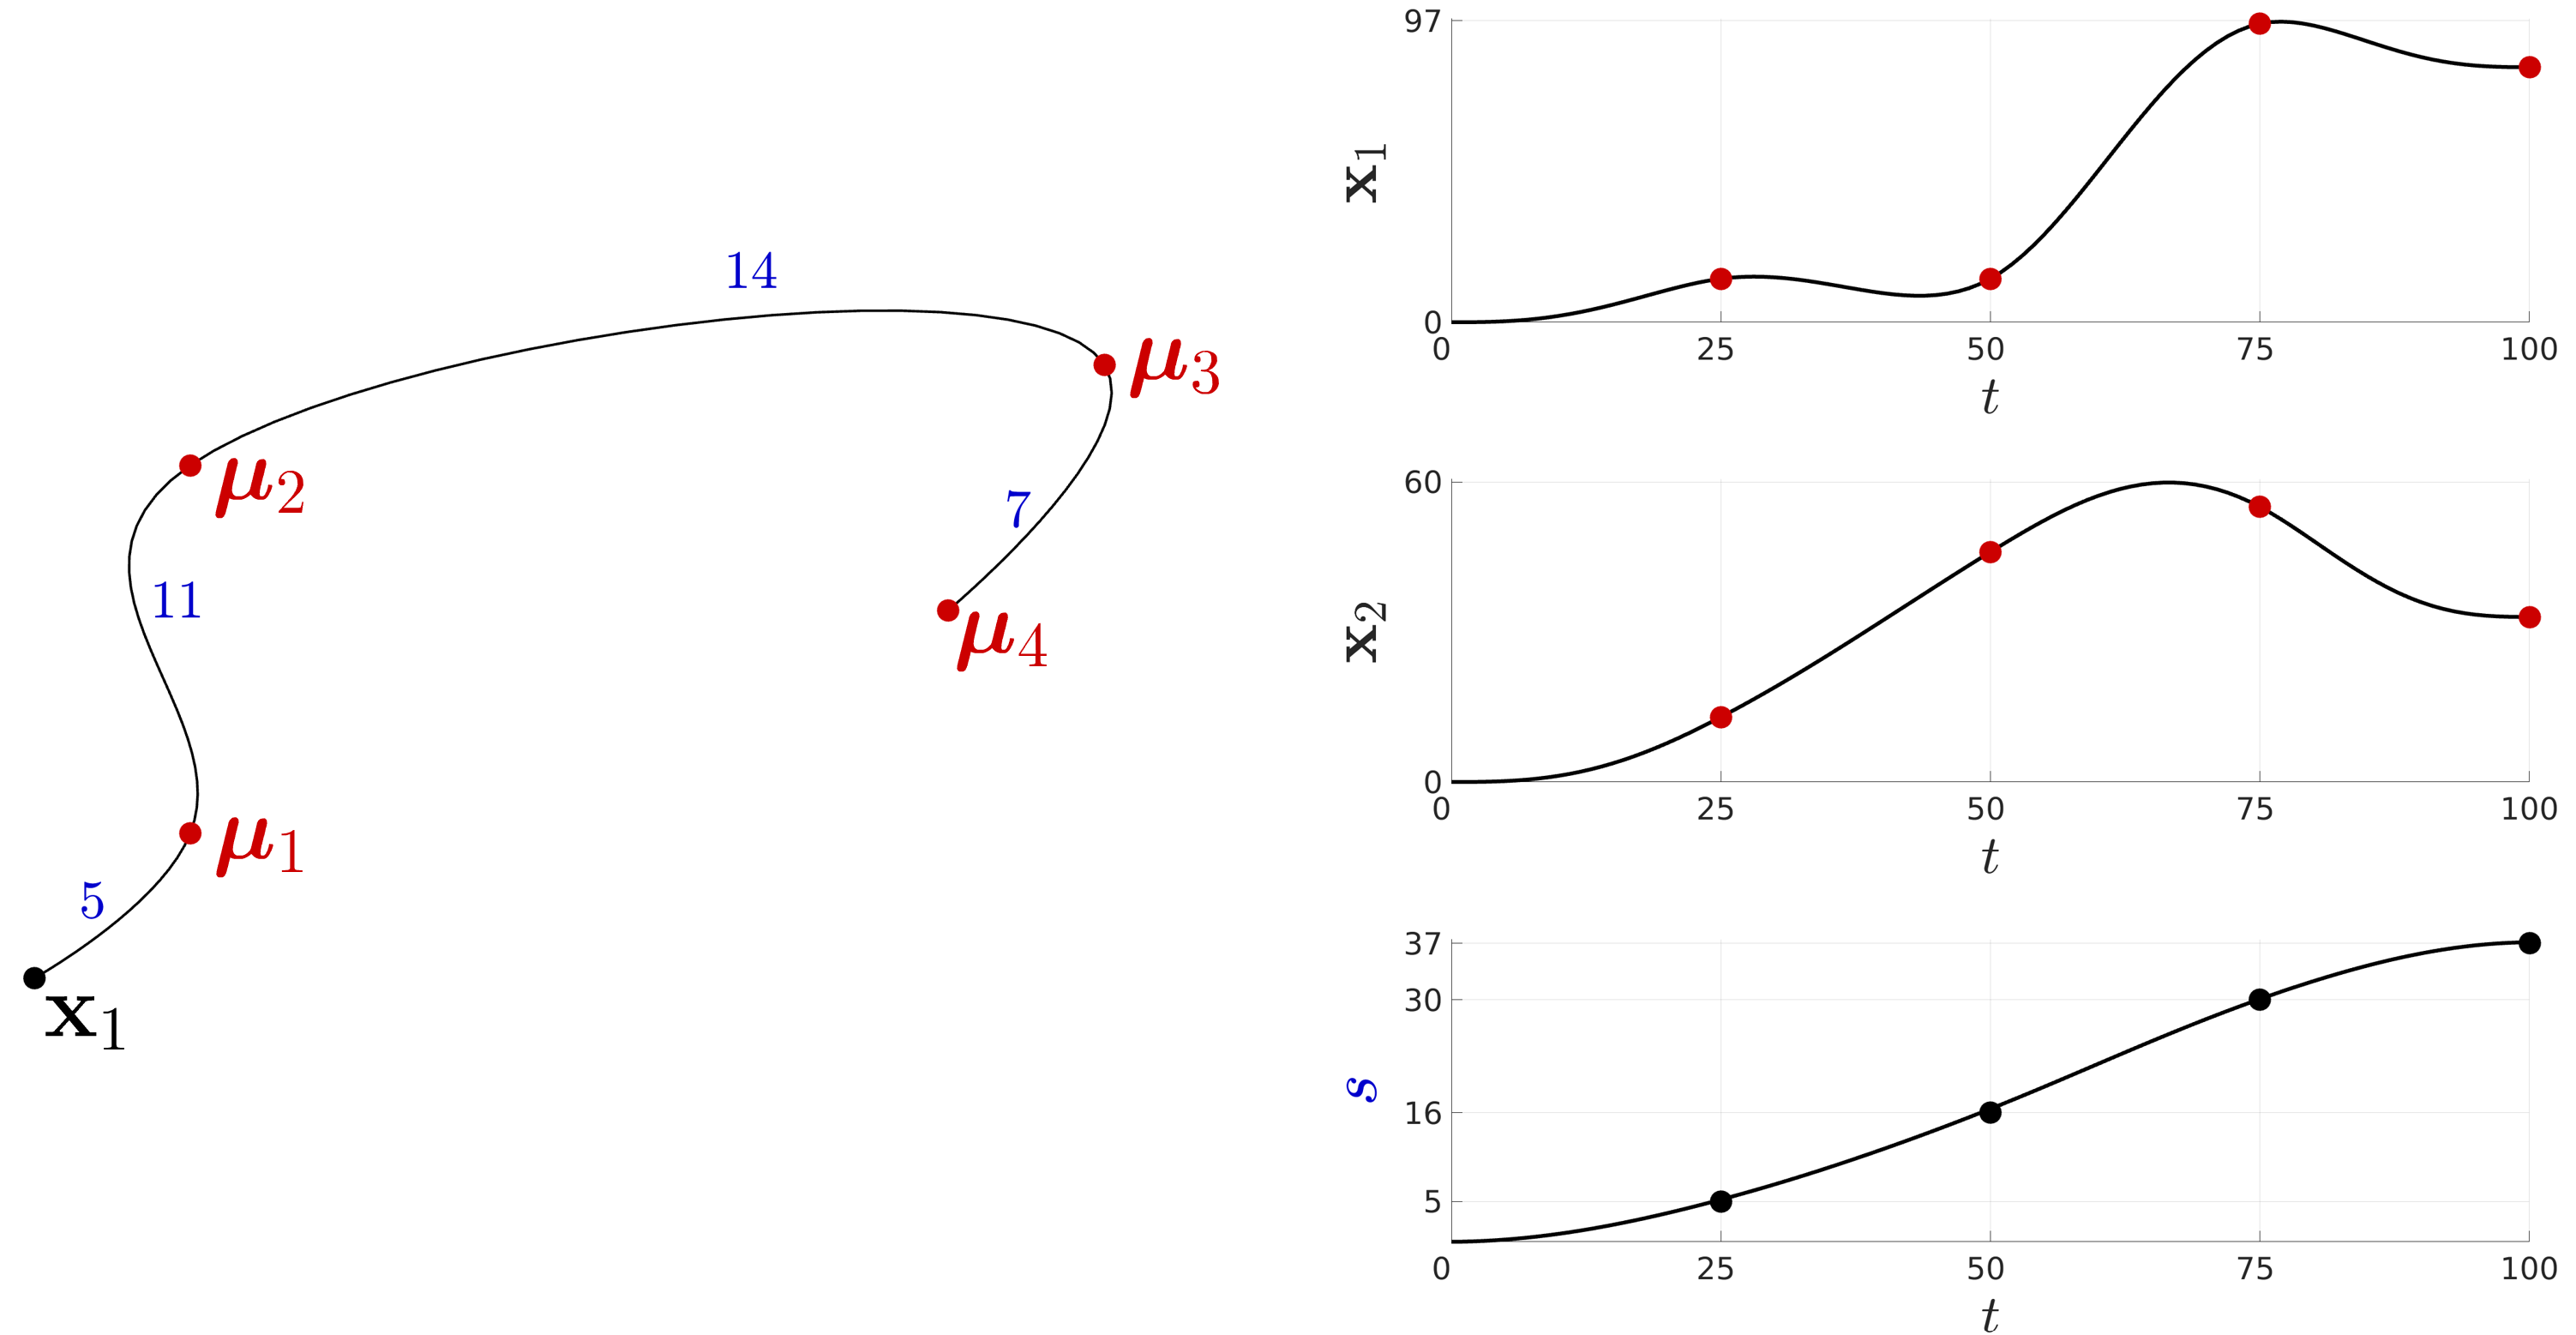
\includegraphics[width=.50\textwidth]{images/iLQR_spacetime01.png}
\caption{\footnotesize
Spacetime optimization with iLQR for a viapoints task, where the estimated durations between consecutive viapoints are shown in blue. 
}
\label{fig:iLQR_spacetime}
\vspace{-60pt}
\end{wrapfigure}

We define a phase variable $s_t$ starting from $s_1=0$ at the beginning of the movement.
With an augmented state $\bm{x}_t={[\mathbf{x}_t^\trsp, s_t]}^\trsp$ and control command $\bm{u}_t={[{\bm{u}^{\mathbf{x}}_t}^\trsp, u^s_t]}^\trsp$, we define the evolution of the system $\bm{x}_{t+1}=\bm{d}(\bm{x}_t,\bm{u}_t)$ as
\begin{align*}
	\mathbf{x}_{t+1} &= \mathbf{A}_t \mathbf{x}_t + \mathbf{B}_t \bm{u}^{\mathbf{x}}_t \, u^s_t,\\
	s_{t+1} &= s_t + u^s_t. % \, \Delta t.
\end{align*}

Its first order Taylor expansion around $\bm{\hat{x}},\bm{\hat{u}}$ provides the linear system
\begin{align*}
	\underbrace{\begin{bmatrix} \Delta\mathbf{x}_{t+1} \\ \Delta s_{t+1} \end{bmatrix}}_{\Delta\bm{x}_{t+1}}
 	&=
	\underbrace{\begin{bmatrix} \mathbf{A}_t & \bm{0} \\ \bm{0} & 1 \end{bmatrix}}_{\bm{A}_t}
	\underbrace{\begin{bmatrix} \Delta\mathbf{x}_t \\ \Delta s_t \end{bmatrix}}_{\Delta\bm{x}_t}
	+
	\underbrace{\begin{bmatrix} \mathbf{B}_t u^s_t & \mathbf{B}_t \bm{u}^{\mathbf{x}}_t \\ \bm{0} & 1 \end{bmatrix}}_{\bm{B}_t} %\Delta t
	\underbrace{\begin{bmatrix} \Delta\bm{u}^{\mathbf{x}}_t \\ \Delta u^s_t \end{bmatrix}}_{\Delta\bm{u}_t},
\end{align*}
with Jacobian matrices $\bm{A}_t \!=\! \frac{\partial\bm{d}}{\partial\bm{x}_t}$, $\bm{B}_t \!=\! \frac{\partial\bm{d}}{\partial\bm{u}_t}$. Note that in the above equations, we used here the notation $\mathbf{x}_t$ and $\bm{x}_t$ to describe the standard state and augmented state, respectively. We similarly used $\{\mathbf{A}_t,\mathbf{B}_t\}$ and $\{\bm{A}_t,\bm{B}_t\}$ (with slanted font) for standard linear system and augmented linear system.

Figure \ref{fig:iLQR_spacetime} shows a viapoints task example in which both path and duration are optimized (convergence after 10 iterations when starting from zero commands). The example uses a double integrator as linear system defined by constant $\mathbf{A}_t$ and  $\mathbf{B}_t$ matrices.

\newpage

%%%%%%%%%%%%%%%%%%%%%%%%%%%%%%%%%%%%%%%%%%%%%%%%%%%%%%%%%%%%%%%%%%%%%%%%%%%%%%%%%
\subsection{iLQR with offdiagonal elements in the precision matrix} 
\begin{flushright}
\filename{iLQR\_manipulator\_object\_affordance.*}
\end{flushright}

\begin{SCfigure}[50]
\centering
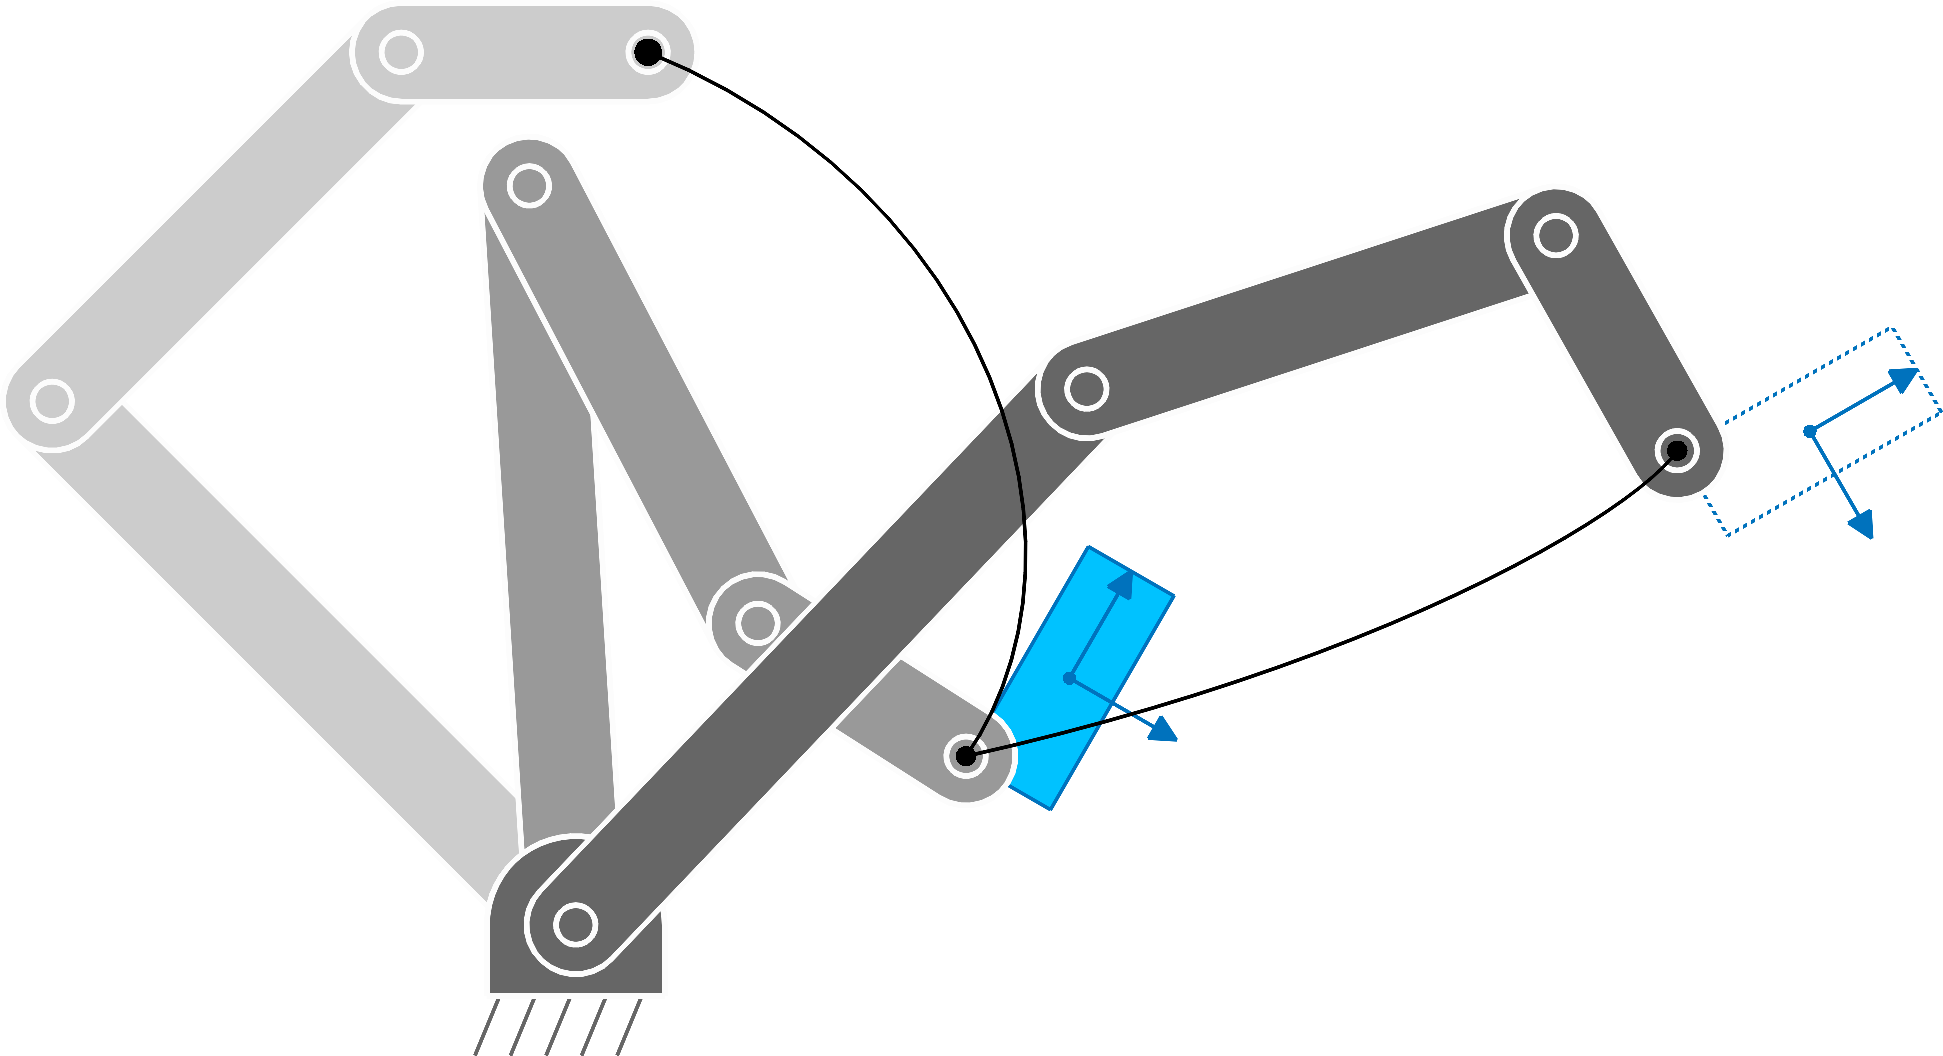
\includegraphics[width=.3\textwidth]{images/iLQR_objAffordances01.png}\hspace{5mm}
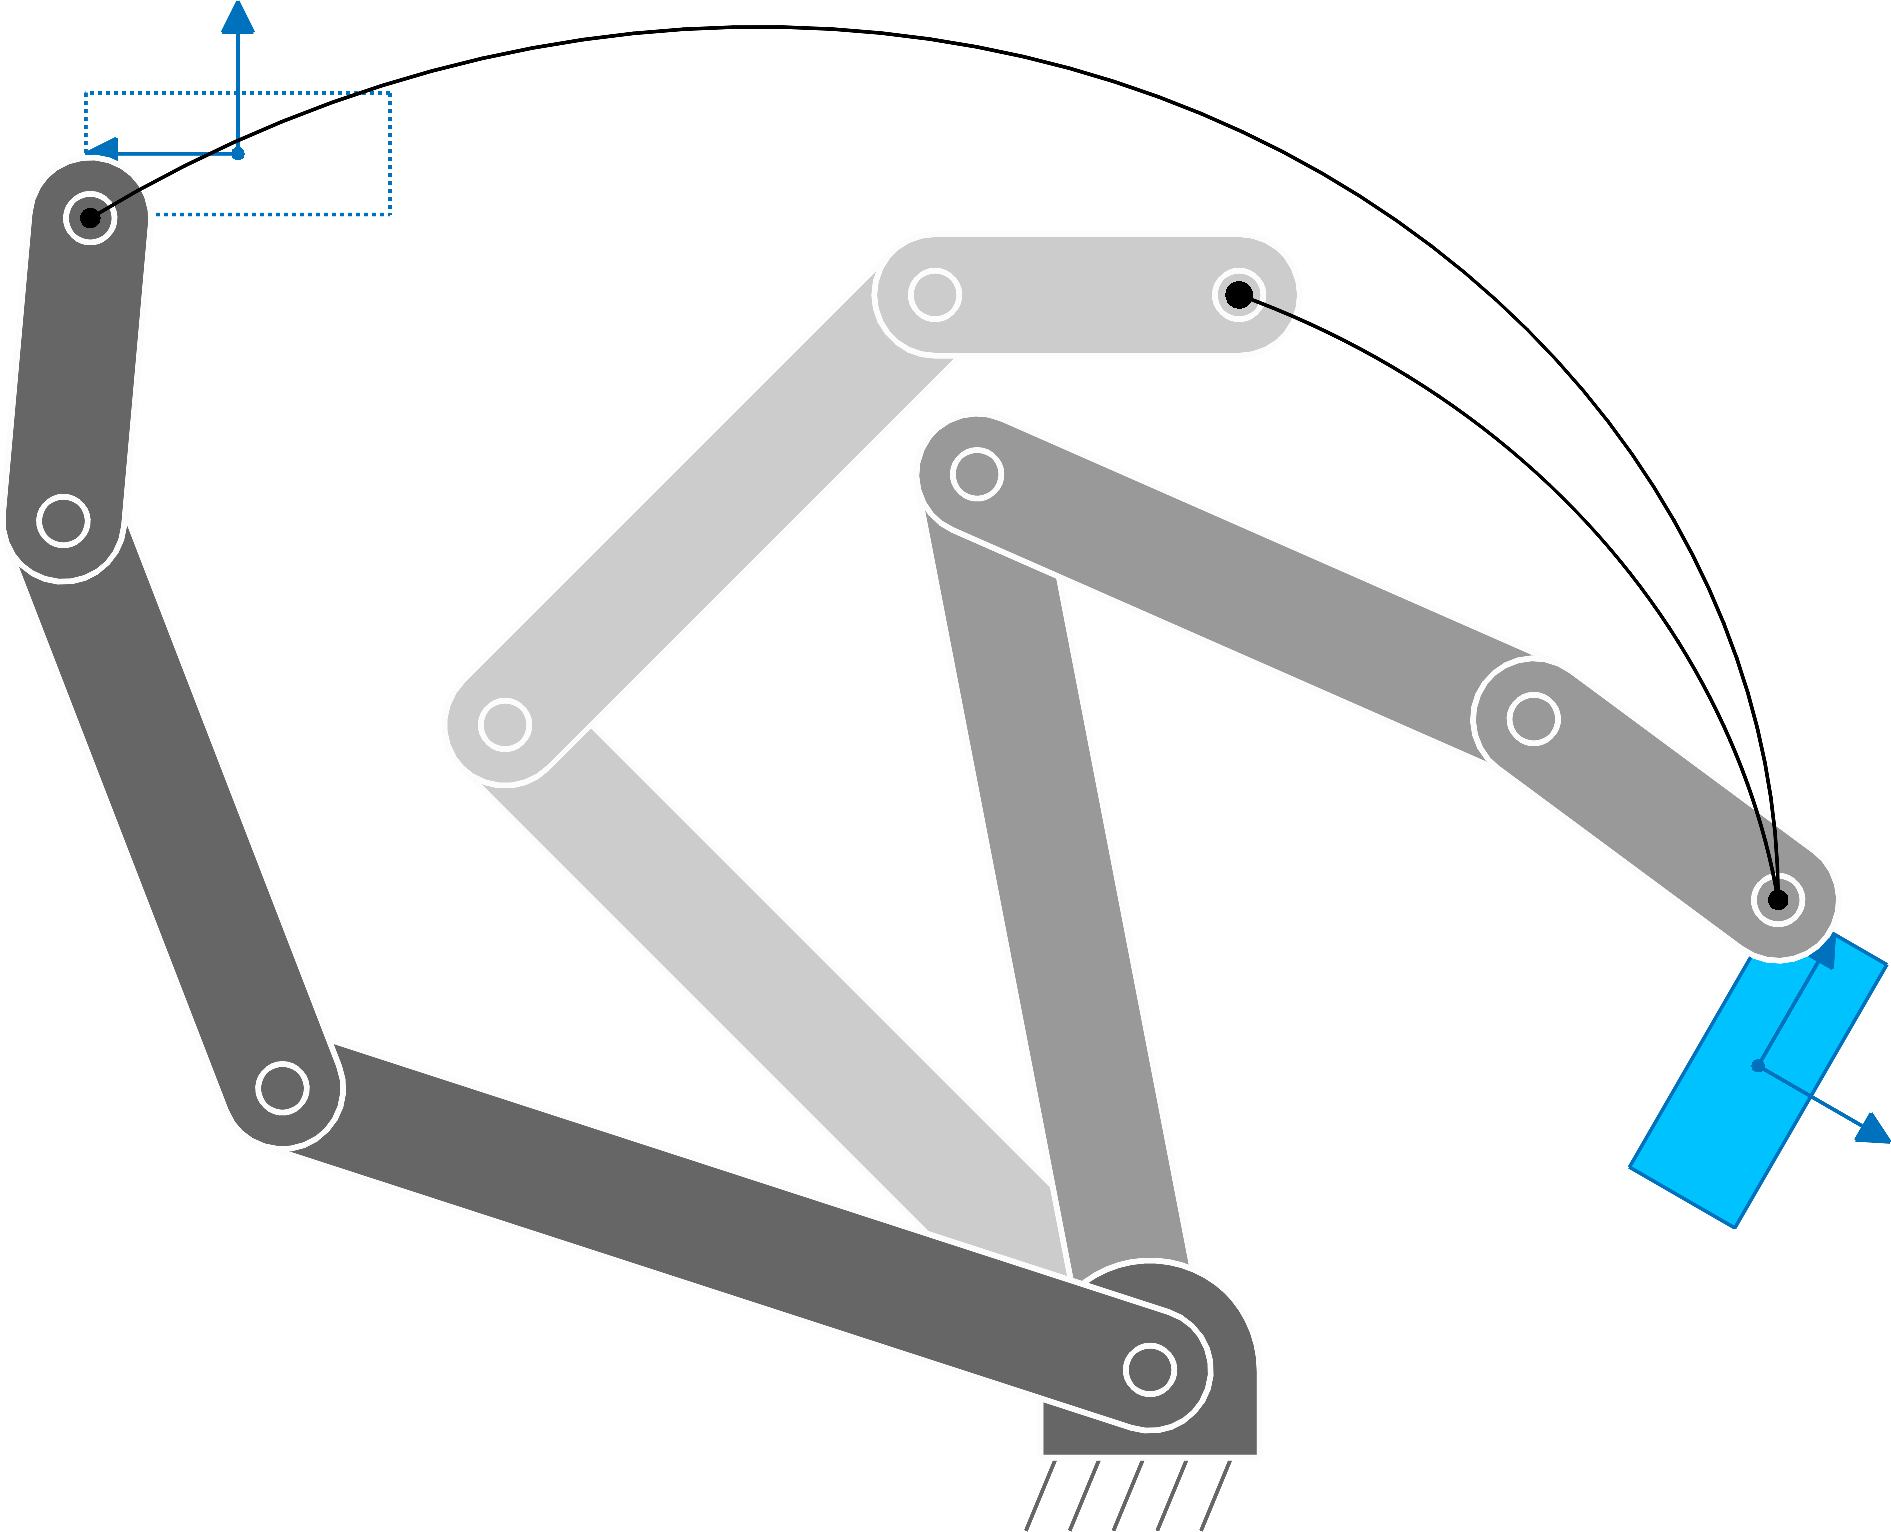
\includegraphics[width=.2\textwidth]{images/iLQR_objAffordances02.png}\vspace{15mm}
\caption{\footnotesize
Manipulation with object affordances cost. The depicted \emph{pick-and-place} task requires the offset at the picking location to be the same as the offset at the placing location, which can be achieved by setting a precision matrix with nonzero offdiagonal entries, see main text for details. In this example, an additional cost is set for choosing the picking and placing points within the object boundaries, which was also used for the task depicted in Fig.~\ref{fig:iLQR_manipulator}. We can see with the resulting motions that when picking the object, the robot anticipates what will be done later with this object, which can be viewed as a basic form of object affordance. In the two situations depicted in the figure, the robot efficiently chooses a grasping point close to one of the corners of the object, different in the two situations, so that the robot can bring the object at the desired location with less effort and without reaching joint angle limits.
}
\label{fig:iLQR_manipulator_objAffordances}
\end{SCfigure}

Spatial and/or temporal constraints can be considered by setting $\left[\begin{smallmatrix}\bm{I}&-\bm{I}\\-\bm{I}&\bm{I}\end{smallmatrix}\right]$ in the corresponding entries of the precision matrix $\bm{Q}$. With this formulation, we can constrain two positions to be the same without having to predetermine the position at which the two should meet. Indeed, we can see that a cost $c\!=\!\left[\begin{smallmatrix}x_i\\x_j\end{smallmatrix}\right]^\trsp\left[\begin{smallmatrix}1&-1\\-1&1\end{smallmatrix}\right]\left[\begin{smallmatrix}x_i\\x_j\end{smallmatrix}\right]\!=\!(x_i-x_j)^2$ is minimized when $x_i\!=\!x_j$.

Such cost can for example be used to define costs on object affordances, see Fig.~\ref{fig:iLQR_manipulator_objAffordances} for an example.


%%%%%%%%%%%%%%%%%%%%%%%%%%%%%%%%%%%%%%%%%%%%%%%%%%%%%%%%%%%%%%%%%%%%%%%%%%%%%%%%%
\subsection{Car steering}
\begin{flushright}
\filename{iLQR\_car.*}
\end{flushright}

\begin{figure}
\centering
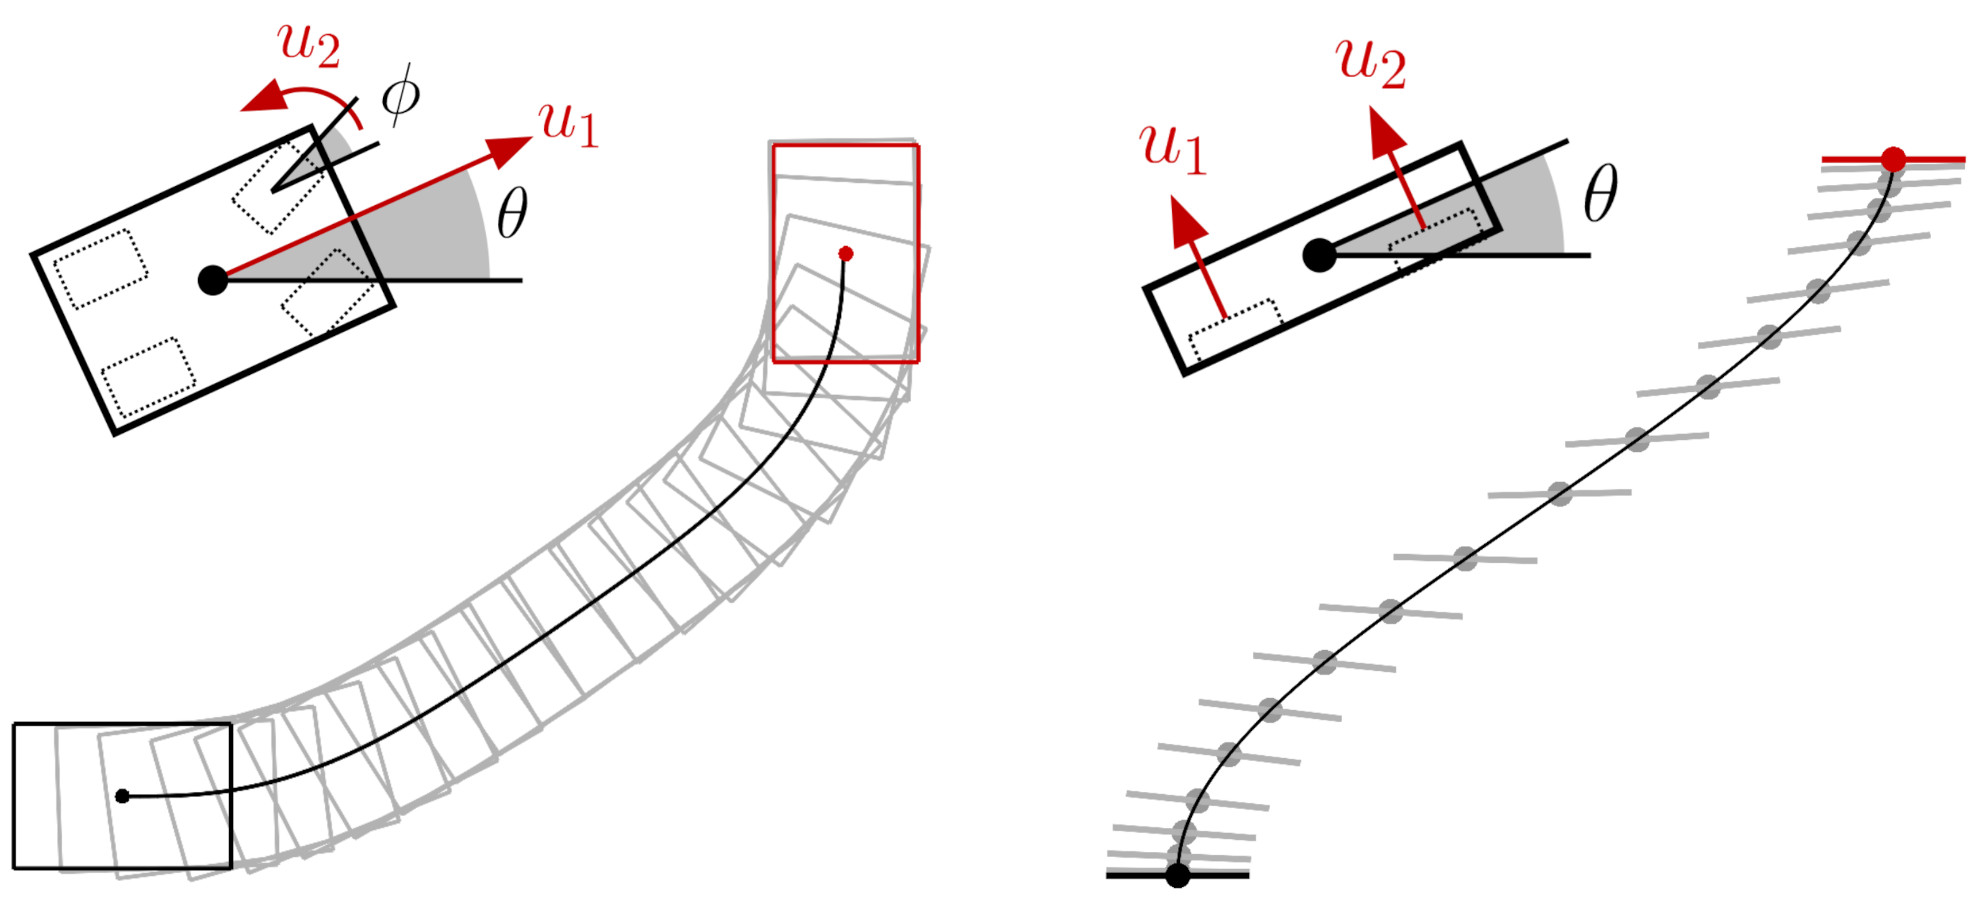
\includegraphics[width=.6\columnwidth]{images/car-bicopter01.jpg}
\caption{\footnotesize
iLQR for car and bicopter control/planning problems.
}
\label{fig:iLQR_car_bicopter}
\end{figure}

\noindent\textbf{Velocity Control Input} \newline
%
A car motion with position $(x_1,x_2)$, car orientation $\theta$, and front wheels orientation $\phi$ (see Fig.~\ref{fig:iLQR_car_bicopter}-\emph{left}) is characterized by equations
\begin{equation*}
	\dot{x}_1 = u_1 \cos(\theta),\quad
	\dot{x}_2 = u_1 \sin(\theta),\quad
	\dot{\theta} = \frac{u_1}{\ell} \tan(\phi),\quad
	\dot{\phi} = u_2,
\end{equation*}
where $\ell$ is the distance between the front and back axles, $u_1$ is the back wheels velocity command and $u_2$ is the front wheels steering velocity command. 
Its first order Taylor expansion around $(\hat{\theta}, \hat{\phi}, \hat{u}_1)$ is
\begin{equation}
	\setlength\arraycolsep{2pt}
	\footnotesize %\scriptsize %\tiny
	\begin{bmatrix} \Delta\dot{x}_1 \\ \Delta\dot{x}_2 \\ \Delta\dot{\theta} \\ \Delta\dot{\phi} \end{bmatrix} =
	\begin{bmatrix} 0 & 0 & -\hat{u}_1\sin(\hat{\theta}) & 0 \\
					0 & 0 & \hat{u}_1\cos(\hat{\theta}) & 0 \\
					0 & 0 & 0 & \frac{\hat{u}_1}{\ell} (\tan(\hat{\phi})^2 \!+\! 1) \\
					0 & 0 & 0 & 0
	\end{bmatrix} 
	\begin{bmatrix} \Delta x_1 \\ \Delta x_2 \\ \Delta\theta \\ \Delta\phi \end{bmatrix} 
	+ 
	\setlength\arraycolsep{2pt}
	\footnotesize %\scriptsize %\tiny
	\begin{bmatrix} \cos(\hat{\theta}) & 0 \\
					\sin(\hat{\theta}) & 0 \\
					\frac{1}{\ell} \tan(\hat{\phi}) & 0 \\
					0 & 1
	\end{bmatrix} 
	\begin{bmatrix} \Delta u_1 \\ \Delta u_2 \end{bmatrix},
\end{equation}
which can then be converted to a discrete form with \eqref{eq:AdAc}. \newline


\noindent\textbf{Acceleration Control Input}\newline
%
A car motion with position $(x_1,x_2)$, car orientation $\theta$, and front wheels orientation $\phi$ (see Fig.~\ref{fig:iLQR_car_bicopter}-\emph{left}) is characterized by equations
\begin{equation*}
	\dot{x}_1 = v \cos(\theta),\quad
	\dot{x}_2 = v \sin(\theta),\quad
	\dot{\theta} = \frac{v}{\ell} \tan(\phi),\quad
	\dot{v} = u_1,\quad
	\dot{\phi} = u_2,
\end{equation*}
where $\ell$ is the distance between the front and back axles, $u_1$ is the back wheels acceleration command and $u_2$ is the front wheels steering velocity command. 
Its first order Taylor expansion around $(\hat{\theta}, \hat{\phi}, \hat{v})$ is
\begin{equation}
	\setlength\arraycolsep{2pt}
	\footnotesize %\scriptsize %\tiny
	\begin{bmatrix} \Delta\dot{x}_1 \\ \Delta\dot{x}_2 \\ \Delta\dot{\theta} \\ \Delta\dot{v} \\ \Delta\dot{\phi} \end{bmatrix} =
	\begin{bmatrix} 0 & 0 & -\hat{v}\sin(\hat{\theta}) & \cos(\hat{\theta}) & 0 \\
					0 & 0 & \hat{v}\cos(\hat{\theta}) & \sin(\hat{\theta}) & 0 \\
					0 & 0 & 0 & \frac{1}{\ell} \tan(\hat{\phi}) & \frac{\hat{v}}{\ell} (\tan(\hat{\phi})^2 \!+\! 1) \\
					0 & 0 & 0 & 0 & 0 \\
					0 & 0 & 0 & 0 & 0
	\end{bmatrix} 
	\begin{bmatrix} \Delta x_1 \\ \Delta x_2 \\ \Delta\theta \\ \Delta v \\ \Delta\phi \end{bmatrix} 
	+ 
	\setlength\arraycolsep{2pt}
	\footnotesize %\scriptsize %\tiny
	\begin{bmatrix} 0 & 0 \\
					0 & 0 \\
					0 & 0 \\
					1 & 0 \\
					0 & 1
	\end{bmatrix} 
	\begin{bmatrix} \Delta u_1 \\ \Delta u_2 \end{bmatrix},
\end{equation}
which can then be converted to a discrete form with \eqref{eq:AdAc}.


%%%%%%%%%%%%%%%%%%%%%%%%%%%%%%%%%%%%%%%%%%%%%%%%%%%%%%%%%%%%%%%%%%%%%%%%%%%%%%%%%
\subsection{Bicopter}
\begin{flushright}
\filename{iLQR\_bicopter.*}
\end{flushright}

A planar bicopter of mass $m$ and inertia $I$ actuated by two propellers at distance $\ell$ (see Fig.~\ref{fig:iLQR_car_bicopter}-\emph{right}) is characterized by equations
\begin{equation*}
	\ddot{x}_1 = -\frac{1}{m} (u_1 + u_2) \sin(\theta),\quad
	\ddot{x}_2 = \frac{1}{m} (u_1 + u_2) \cos(\theta) - g,\quad
	\ddot{\theta} = \frac{\ell}{I} (u_1 - u_2),
\end{equation*}
with acceleration $g\!=\!9.81$ due to gravity. Its first order Taylor expansion around $(\hat{\theta},\hat{u}_2,\hat{u}_2)$ is
\begin{equation}
	\setlength\arraycolsep{2pt}
	\footnotesize %\scriptsize %\tiny
	\begin{bmatrix} \Delta\dot{x}_1 \\ \Delta\dot{x}_2 \\ \Delta\dot{\theta} \\ \Delta\ddot{x}_1 \\ \Delta\ddot{x}_2 \\ \Delta\ddot{\theta} \end{bmatrix} =
	\begin{bmatrix} 0 & 0 & 0 & 1 & 0 & 0 \\ 
					0 & 0 & 0 & 0 & 1 & 0 \\
					0 & 0 & 0 & 0 & 0 & 1 \\
					0 & 0 & -\frac{1}{m} (\hat{u}_1 + \hat{u}_2) \cos(\hat{\theta}) & 0 & 0 & 0 \\
					0 & 0 & -\frac{1}{m} (\hat{u}_1 + \hat{u}_2) \sin(\hat{\theta}) & 0 & 0 & 0 \\
					0 & 0 & 0 & 0 & 0 & 0 
	\end{bmatrix} 
	\begin{bmatrix} \Delta x_1 \\ \Delta x_2 \\ \Delta\theta \\ \Delta\dot{x}_1 \\ \Delta\dot{x}_2 \\ \Delta\dot{\theta} \end{bmatrix}
	+ 
	\setlength\arraycolsep{2pt}
	\footnotesize %\scriptsize %\tiny
	\begin{bmatrix} 0 & 0 \\ 0 & 0 \\ 0 & 0 \\ 
	-\frac{1}{m} \sin(\hat{\theta}) & -\frac{1}{m} \sin(\hat{\theta}) \\ 
	\frac{1}{m} \cos(\hat{\theta}) & \frac{1}{m} \cos(\hat{\theta}) \\ 
	\frac{\ell}{I} & -\frac{\ell}{I} \end{bmatrix} 
	\begin{bmatrix} \Delta u_1 \\ \Delta u_2 \end{bmatrix},
\end{equation}
which can then be converted to a discrete form with \eqref{eq:AdAc}.



%%%%%%%%%%%%%%%%%%%%%%%%%%%%%%%%%%%%%%%%%%%%%%%%%%%%%%%%%%%%%%%%%%%%%%%%%%%%%%%%%
%\subsection{iLQR with quadratic cost function}

%If the cost function is already quadratic, with
%\begin{equation}
%	c(\bm{x}_t,\bm{u}_t) = {(\bm{x}_t-\bm{\mu}_t)}^\trsp \bm{Q}_t (\bm{x}_t-\bm{\mu}_t) + \bm{u}_t^\trsp \bm{R}_t \, \bm{u}_t, 
%\end{equation}
%we have %see e.g. (85) (or (78), or (97)) in the Matrix Cookbook 
%\begin{equation*}
%	\bm{g}_{\bm{x}_t} \!=\! \frac{\partial c}{\partial\bm{x}_t} = 2 \bm{Q}_t (\bm{x}_t-\bm{\mu}_t),\quad
%	\bm{g}_{\bm{u}_t} \!=\! \frac{\partial c}{\partial\bm{u}_t} = 2 \bm{R}_t \bm{u}_t,
%\end{equation*}
%\begin{equation*}
%	\bm{H}_{\bm{x}_t} \!\!=\!\! \frac{\partial^2 c}{\partial\bm{x}_t^2} \!=\! 2 \bm{Q}_t, \;
%	\bm{H}_{\bm{x}_t\!\bm{u}_t} \!\!=\!\! \frac{\partial^2 c}{\partial\bm{x}_t\bm{u}_t} \!=\! \bm{0}, \;
%	\bm{H}_{\bm{u}_t} \!\!=\!\! \frac{\partial^2 c}{\partial\bm{u}_t^2} \!=\! 2 \bm{R}_t,
%\end{equation*}
%and the second-order Taylor expansion in \eqref{eq:dc} then becomes 
%\begin{multline}
%	\Delta c(\Delta\bm{x}_t,\Delta\bm{u}_t) \approx \Delta\bm{x}_t^\trsp 2 \bm{Q}_t (\bm{x}_t-\bm{\mu}_t) + \Delta\bm{u}_t^\trsp 2 \bm{R}_t \, \bm{u}_t +\\
%	\Delta\bm{x}_t^\trsp \bm{Q}_t \Delta\bm{x}_t + \Delta\bm{u}_t^\trsp \bm{R}_t \Delta\bm{u}_t.
%	\label{eq:dcquad}
%\end{multline}

%At a trajectory level, the minimization problem can be rewritten in batch form as
%\begin{align}
%	\min_{\Delta\bm{u}} & \; \Delta\bm{x}^{\!\trsp} 2 \bm{Q} \, (\bm{x}\!-\!\bm{\mu}) + \Delta\bm{u}^{\!\trsp} 2 \bm{R} \, \bm{u} +
%	\Delta\bm{x}^{\!\trsp} \bm{Q} \, \Delta\bm{x} + \Delta\bm{u}^{\!\trsp} \bm{R} \, \Delta\bm{u}, \nonumber\\
%	\text{s.t.} & \; \Delta\bm{x} = \bm{S}_{\bm{x}} \Delta\bm{x}_1 + \bm{S}_{\bm{u}} \Delta\bm{u}.
%\end{align}

%By inserting the constraint into the cost we have
%\begin{multline}
%	\Delta c(\Delta\bm{x},\Delta\bm{u}) \approx 
%	(\bm{S}_{\bm{x}} \Delta\bm{x}_1 + \bm{S}_{\bm{u}} \Delta\bm{u})^\trsp 2 \bm{Q} (\bm{x}-\bm{\mu}) + \Delta\bm{u}^{\!\trsp} 2 \bm{R} \, \bm{u} + \\ 
%	(\bm{S}_{\bm{x}} \Delta\bm{x}_1 + \bm{S}_{\bm{u}} \Delta\bm{u})^{\!\trsp} \bm{Q} (\bm{S}_{\bm{x}} \Delta\bm{x}_1 + \bm{S}_{\bm{u}} \Delta\bm{u}) + 
%	\Delta\bm{u}^\trsp \bm{R} \Delta\bm{u},
%\end{multline}
%which can be solved analytically by differentiating with respect to $\Delta\bm{u}$ and equating to zero, namely,
%\begin{multline}	
%	2 \bm{S}_{\bm{u}}^\trsp \bm{Q} (\bm{x}-\bm{\mu}) + 2 \bm{R} \, \bm{u} + 
%	2 \bm{S}_{\bm{u}}^\trsp \bm{Q} \bm{S}_{\bm{x}} \Delta\bm{x}_1 + \\
%	2 \bm{S}_{\bm{u}}^\trsp \bm{Q} \bm{S}_{\bm{u}} \Delta\bm{u} +
%	2 \bm{R} \Delta\bm{u} = \bm{0},
%\end{multline}
%providing the least squares solution
%\begin{equation}
%	\Delta\bm{\hat{u}} = {\big(\bm{S}_{\bm{u}}^\trsp \bm{Q} \bm{S}_{\bm{u}} \!+\! \bm{R}\big)}^{\!-1}
%	\big(\bm{S}_{\bm{u}}^\trsp \bm{Q} (\bm{\mu} - \bm{x}) - \bm{R} \, \bm{u} - \bm{S}_{\bm{u}}^\trsp \bm{Q} \bm{S}_{\bm{x}} \Delta\bm{x}_1 \big),
%	\label{eq:duh}
%\end{equation}
%which can be used to update the control commands estiamte at each iteration step of the iLQR algorithm.

%Since in our problem, we start from $\Delta\bm{x}_1=\bm{0}$, \eqref{eq:duh} can be further simplified to
%\begin{equation}
%	\Delta\bm{\hat{u}} = {\big(\bm{S}_{\bm{u}}^\trsp \bm{Q} \bm{S}_{\bm{u}} \!+\! \bm{R}\big)}^{\!-1}
%	\big(\bm{S}_{\bm{u}}^\trsp \bm{Q} \, (\bm{\mu} - \bm{x}) - \bm{R} \, \bm{u} \big).
%	\label{eq:du}
%\end{equation}


%%%%%%%%%%%%%%%%%%%%%%%%%%%%%%%%%%%%%%%%%%%%%%%%%%%%%%%%%%%%%%%%%%%%%%%%%%%%%%%%%
\section{Ergodic control}\label{sec:ergodicControl}

\begin{center}
\includegraphics[width=.7\columnwidth]{images/ergodic01.png}
\end{center}

A conventional tracking problem in robotics is characterized by a target to reach, requiring a controller to be computed to reach this target. In \emph{ergodic control}, instead of providing a single target point, a probability distribution is given to the robot, which must cover the distribution in an efficient way. Ergodic control thus consists of moving within a spatial distribution by spending time in each part of the distribution in proportion to its density (namely, ``tracking a distribution'' instead of ``tracking a point''). The resulting controller generates natural exploration behaviors, which can be exploited for active sensing, localization, surveillance, insertion tasks, etc. 

In robotics, ergodic control can be exploited in a wide range of problems requiring the automatic exploration of regions of interest. This is particularly helpful when the available sensing information is not accurate enough to fulfill the task with a standard controller, but where this information can still guide the robot towards promising areas. In a collaborative task, it can also be used when the operator's input is not accurate enough to fully reproduce the task, which then requires the robot to explore around the requested input (e.g., a point of interest selected by the operator). For picking and insertion problems, ergodic control can be applied to move around the picking/insertion point, thereby facilitating the prehension/insertion. It can also be employed for active sensing and localization (either detected autonomously, or with help by the operator). Here, the robot can plan movements based on the current information density, and can recompute the commands when new measurements are available (i.e., updating the spatial distribution used as target). 

Ergodic control is originally formulated as a \emph{spectral multiscale coverage} (SMC) objective \cite{Mathew09}, which we will see next. Other ergodic control techniques have later been proposed, including the \emph{heat equation driven area coverage} (HEDAC) \cite{Ivic17}, which we will also be introduced next.


%%%%%%%%%%%%%%%%%%%%%%%%%%%%%%%%%%%%%%%%%%%%%%%%%%%%%%%%%%%%%%%%%%%%%%%%%%%%%%%%%
\subsection{Spectral multiscale coverage (SMC)}\label{sec:SMC}
\begin{flushright}
\filename{ergodic\_control\_SMC.*}
\end{flushright}

The underlying objective of \emph{spectral multiscale coverage} (SMC) takes a simple form, corresponding to a tracking problem in the spectral domain (tracking of frequency components) \cite{Mathew09}. The advantage of such a control formulation is that it can be easily combined with other control objectives and constraints.

It requires the spatial distribution to be decomposed as Fourier series, with a cost function comparing the spectral decomposition of the robot path with the spectral decomposition of the distribution. The resulting controller allows the robot to explore the given spatial distribution in a natural manner, \textbf{by starting from a crude exploration and by refining the search progressively} (i.e., matching the Fourier coefficients with an increasing importance from low to high frequency components). 

%% Fourier basis functions
We will adopt a notation to make links with the superposition of basis functions seen in Section \ref{sec:basisfcts}. By starting with the unidimensional case, we will consider a signal $g(x)$ varying along a variable $x$, where $x$ will be used as a generic variable that can for example be a time variable or the coordinates of a pixel in an image. The signal $g(x)$ can be approximated as a weighted superposition of basis functions with 
\begin{align*}
	g(x) &= \sum_{k=-K\!+\!1}^{K\!-\!1} w_k \, \phi_k(x)\\
	&= \bm{w}^\trsp \bm{\phi}(x), 
\end{align*}
where $\bm{w}$ and $\bm{\phi}(x)$ are vectors formed with the elements of $w_k$ and $\phi_k(x)$, respectively.
$w_k$ and $\phi_k(x)$ denote the coefficients and basis functions of the Fourier series, with
\begin{align}
	\phi_k(x) &= \frac{1}{L} \exp\!\left(-i\frac{2\pi k x}{L}\right)\nonumber\\
	&= \frac{1}{L} \Bigg(\!\cos\!\left(\frac{2\pi k x}{L}\right) - i \, \sin\!\left(\frac{2\pi k x}{L}\right) \!\Bigg)
	, \;\forall k\!\in\![-K\!+\!1,\ldots,K\!-\!1],
	\label{eq:complExp1D}
\end{align}
with $i$ the imaginary unit of a complex number ($i^2=-1$).

The use of Fourier basis functions provides useful connections between the spatial domain and the frequency domain. Several Fourier series properties can be exploited, notably regarding zero-centered Gaussians, shift, symmetry, and linear combination. 
These properties are reported in Table \ref{tab:Fourier} for the 1D case.

\begin{table*}
\caption{Fourier series properties (1D case).}
\label{tab:Fourier}
\begin{mdframed}

\noindent\textbf{Symmetry property:}\\
If $g(x)$ is real and even, $\phi_k(x)$ in \eqref{eq:complExp1D} is also real and even, simplifying to $\phi_k(x) = \frac{1}{L} \cos\!\left(\frac{2\pi k x}{L}\right)$, which then, in practice, only needs an evaluation on the range $k\!\in\![0,\ldots,K\!-\!1]$, as the basis functions are even. We then have $g(x) = w_0 + \sum_{k=1}^{K\!-\!1} w_k \, 2\cos\!\left(\frac{2\pi k x}{L}\right)$, by exploiting $\cos(0)\!=\!1$.\\[-2mm]

\noindent\textbf{Shift property:}\\
If $w_k$ are the Fourier series coefficients of a function $g(x)$, $\exp(-i \frac{2\pi k \mu}{L}) w_k$ are the Fourier coefficients of $g(x-\mu)$.\\[-2mm]

\noindent\textbf{Combination property:}\\
If $w_{k,1}$ (resp.\ $w_{k,2}$) are the Fourier series coefficients of a function $g_1(x)$ (resp.\ $g_2(x)$), then $\alpha_1 w_{k,1}+\alpha_2 w_{k,2}$ are the Fourier coefficients of $\alpha_1 g_1(x)+\alpha_2 g_2(x)$.\\[-2mm]

\noindent\textbf{Gaussian property:}\\
If $g_0(x)=\mathcal{N}(x \,|\, 0, \sigma^2)=(2\pi\sigma^2)^{-\frac{1}{2}} \exp(-\frac{x^2}{2\sigma^2})$
is mirrored to create a real and even periodic function $g(x)$ of period $L\gg\sigma$ (implementation details will follow), the corresponding Fourier series coefficients are of the form $w_k=\exp(-\frac{2\pi^2 k^2 \sigma^2}{L^2})$.\\[-2mm]

\end{mdframed}
\end{table*}

\begin{figure}
\centering{\includegraphics[width=.7\columnwidth]{images/ergodicControl02.png}}
\caption{
2D ergodic control based on SMC used to generate search behaviors.
\emph{(a)} shows the spatial distribution $\hat{g}(\bm{x})$ that the agent has to explore, encoded here as a mixture of two Gaussians (gray colormap in left graph). The right graphs show the corresponding Fourier series coefficients $\hat{w}_{\bm{k}}$ in the frequency domain ($K=9$ coefficients per dimension). \emph{(b)} shows the evolution of the reconstructed spatial distribution $g(\bm{x})$ (left graph) and the computation of the next control command $\bm{u}$ (red arrow) after $T/10$ iterations. The corresponding Fourier series coefficients $w_{\bm{k}}$ are shown in the right graph. \emph{(c)} shows that after $T$ iterations, the agent covers the space in proportion to the desired spatial distribution, with a good match of coefficients in the frequency domain (we can see that $\hat{w}_{\bm{k}}$ and $w_{\bm{k}}$ are nearly the same). \emph{(d)} shows how a periodic signal $\hat{g}(\bm{x})$ (with range $[-L/2,L/2]$ for each dimension) can be constructed from an initial mixture of two Gaussians $\hat{g}_0(\bm{x})$ (red area). The constructed signal $\hat{g}(\bm{x})$ is composed of eight Gaussians in this 2D example, by mirroring the Gaussians along horizontal and vertical axes to construct an even signal of period $L$. \emph{(e)} depicts the first few basis functions of the Fourier series for the first four coefficients in each dimension, represented as a 2D colormap corresponding to periodic signals of different frequencies along two axes.
\label{fig:ergodic_SMC}
}
\end{figure}

Well-known applications of Fourier basis functions in the context of time series include speech processing and the analysis of periodic motions such as gaits. 

In ergodic control, the aim is to find a series of control commands $\bm{u}(t)$ so that the retrieved trajectory $\bm{x}(t)\in\mathbb{R}^D$ covers a bounded space $\mathcal{X}$ in proportion of a desired spatial distribution $\hat{g}(\bm{x})$, see Fig.~\ref{fig:ergodic_SMC}-\emph{(a)}. This can be achieved by defining a metric in the spectral domain, by decomposing in Fourier series coefficients both the desired spatial distribution $\hat{g}(\bm{x})$ and the (partially) retrieved trajectory $\bm{x}(t)$.
The goal of ergodic control is to minimize
\begin{align}
	\epsilon &= \frac{1}{2} \sum_{{\bm{k}}\in\mathcal{K}} \Lambda_{\bm{k}} \Big( w_{\bm{k}} - \hat{w}_{\bm{k}} \Big)^{\!2} \label{eq:ergodicerror}\\
	&= \frac{1}{2} {\Big( \bm{w} - \bm{\hat{w}} \Big)}^{\!\trsp} \bm{\Lambda} \, \Big( \bm{w} - \bm{\hat{w}} \Big),
\end{align}
where $\Lambda_{\bm{k}}$ are weights, $\hat{w}_{\bm{k}}$ are the Fourier series coefficients of $\hat{g}(\bm{x})$, and $w_{\bm{k}}$ are the Fourier series coefficients along the trajectory $\bm{x}(t)$. $\mathcal{K}$ is a set of index vectors in $\mathbb{N}^D$ covering the $D$-dimensional array $\bm{k}=\bm{r}\times\bm{r}\times\cdots\times\bm{r}$, with $\bm{r}=[0,1,\ldots,K\!-\!1]$ and $K$ the resolution of the array.\footnote{For $D=2$ and $K=2$, we have $\mathcal{K}=\big\{\left[\begin{smallmatrix}0\\0\end{smallmatrix}\right],\left[\begin{smallmatrix}0\\1\end{smallmatrix}\right],\left[\begin{smallmatrix}1\\0\end{smallmatrix}\right],\left[\begin{smallmatrix}1\\1\end{smallmatrix}\right]\big\}$.}
$\bm{w}\in\mathbb{R}^{K^D}$ and $\bm{\hat{w}}\in\mathbb{R}^{K^D}$ are vectors composed of elements $w_{\bm{k}}$ and $\hat{w}_{\bm{k}}$, respectively. $\bm{\Lambda}\in\mathbb{R}^{K^D\times K^D}$ is a diagonal weighting matrix with elements $\Lambda_{\bm{k}}$.
In \eqref{eq:ergodicerror}, the weights
\begin{equation}
	\Lambda_{\bm{k}} = \left(1+ \|\bm{k}\|^2\right)^{\!-\frac{D+1}{2}}
\end{equation}
assign more importance on matching low frequency components (related to a metric for Sobolev spaces of negative order). %negative Sobolev norm
The Fourier series coefficients $w_{\bm{k}}$ along a trajectory $\bm{x}(t)$ of continuous duration $t$ are defined as
\begin{equation}
	w_{\bm{k}} = \frac{1}{t} \int_{\tau=0}^t \phi_{\bm{k}}\big(\bm{x}(\tau)\big) \; d\tau,
	\label{eq:ck}
\end{equation}
whose discretized version can be computed recursively at each discrete time step $t$ to build
\begin{equation}
	w_{\bm{k}} = \frac{1}{t} \sum_{s=1}^t \phi_{\bm{k}}(\bm{x}_s), 
\end{equation}
or equivalently in vector form $\bm{w} = \frac{1}{t}\sum_{s=1}^t\bm{\phi}(\bm{x}_s)$. 

For a spatial signal $\bm{x}\in\mathbb{R}^D$, where $x_d$ is on the interval $[-\frac{L}{2},\frac{L}{2}]$ of period $L$, $\forall d\!\in\!\{1,\ldots,D\}$, the basis functions of the Fourier series with complex exponential functions are defined as (see Fig.~\ref{fig:ergodic_SMC}-\emph{(e)})
\begin{align}
	\phi_{\bm{k}}(\bm{x}) &= \frac{1}{L^D} \prod_{d=1}^D \exp\!\left(-i\frac{2\pi k_d x_d}{L}\right)\nonumber\\
	&= \frac{1}{L^D} \prod_{d=1}^D \cos\!\left(\frac{2\pi k_d x_d}{L}\right) - i \, \sin\!\left(\frac{2\pi k_d x_d}{L}\right)
	, \quad\forall\bm{k}\!\in\!\mathcal{K}.
	\label{eq:complExpND}
\end{align}

%% Ergodic controller
Ergodic control is then set as the constrained problem of computing a control command $\bm{\hat{u}}(t)$ at each time step $t$ with 
\begin{equation}
	\bm{\hat{u}}(t) = \arg\min_{\bm{u}(t)}\; \epsilon\big(\bm{x}(t\!+\!\Delta t)\big), 
	\quad \text{s.t.} \quad
	\bm{\dot{x}}(t) = f\big(\bm{x}(t),\bm{u}(t)\big),\quad \|\bm{u}(t)\| \leqslant u^{\max},
	\label{eq:objFct}
\end{equation}
where the simple system $\bm{\dot{x}}(t)=\bm{u}(t)$ is considered (control with velocity commands), and where the error term is approximated with the Taylor series
\begin{equation}
	\epsilon\big(\bm{x}(t\!+\!\Delta t)\big) \;\approx\; \epsilon\big(\bm{x}(t)\big) \;+\; \dot{\epsilon}\big(\bm{x}(t)\big) \Delta t 
	\;+\; \frac{1}{2} \ddot{\epsilon}\big(\bm{x}(t)\big) {\Delta t}^2.
	\label{eq:etpp}
\end{equation}
By using \eqref{eq:ergodicerror}, \eqref{eq:ck}, \eqref{eq:complExpND} and the chain rule $\frac{\partial f}{\partial t}=\frac{\partial f}{\partial \bm{x}} \frac{\partial \bm{x}}{\partial t}$, the Taylor series
is composed of the control term $\bm{u}(t)$ and $\nabla_{\!\!\bm{x}} \phi_{\bm{k}}\big(\bm{x}(t)\big)\in\mathbb{R}^{1\times D}$, the gradient of $\phi_{\bm{k}}\big(\bm{x}(t)\big)$ with respect to $\bm{x}(t)$.
Solving the constrained objective in \eqref{eq:objFct} then results in the analytical solution (see \cite{Mathew09} for the complete derivation)
\begin{align}
	\bm{u} = \bm{\tilde{u}}(t)\frac{u^{\max}}{\|\bm{\tilde{u}}(t)\|},
	\quad\mathrm{with}\quad
	\bm{\tilde{u}} &= -\sum_{{\bm{k}}\in\mathcal{K}} \Lambda_{\bm{k}} \big( w_{\bm{k}} - \hat{w}_{\bm{k}} \big) 
	{\nabla_{\!\!\bm{x}} \phi_{\bm{k}}\big(\bm{x}(t)\big)}^\trsp\nonumber\\
	&= -\bm{\nabla}_{\!\!\bm{x}}\bm{\phi}\big(\bm{x}(t)\big) \; \bm{\Lambda} \, \big( \bm{w} - \bm{\hat{w}} \big),
\end{align}
where $\bm{\nabla}_{\!\!\bm{x}}\bm{\phi}\big(\bm{x}(t)\big)\in\mathbb{R}^{D\times K^D}$ is a concatenation of the vectors $\nabla_{\!\!\bm{x}} \phi_{\bm{k}}\big(\bm{x}(t)\big)$.   

Figure \ref{fig:ergodic_SMC} shows a 2D example of ergodic control to create a motion approximating the distribution given by a mixture of two Gaussians. A remarkable characteristic of such approach is that the controller produces natural exploration behaviors (see Fig.~\ref{fig:ergodic_SMC}-\emph{(c)}) without relying on stochastic noise in the formulation. In the limit case, if the distribution $g(\bm{x})$ is a single Gaussian with a very small isotropic covariance, the controller results in a standard tracking behavior.

%The downside of the original ergodic control approach is that it does not scale well to problems requiring exploration in search space of more than two dimensions. In particular, the original approach would be too slow to consider full distributions in 6D spaces, which would be ideally required. Indeed, both position and orientation of endeffector(s) matter in most robot problems, including manipulation, insertion, welding, or the use of tools at the robot endeffectors. 
%In \cite{Shetty21TRO}, we demonstrated that the original problem formulation can be conserved \textbf{by efficiently compressing the Fourier series decomposition with tensor train (TT) factorization}. The proposed solution is efficient both computationally and storage-wise, hence making it suitable for online implementations, as well as to tackle robot learning problems with a low quantity of training data. The above figure shows an overview of an insertion experiment conducted with the Siemens gears benchmark requiring full 6D endeffector poses. Further work is required to extend the approach to online active sensing applications in which the distributions can change based on the data collected by ergodic control. 

\newpage

%%%%%%%%%%%%%%%%%%%%%%%%%%%%%%%%%%%%%%%%%%%%%%%%%%%%%%%%%%%%%%%%%%%%%%%%%%%%%%%%%
\subsection{Heat equation driven area coverage (HEDAC)}\label{sec:HEDAC}
\begin{flushright}
\filename{ergodic\_control\_HEDAC.*}
\end{flushright}

Heat equation driven area coverage (HEDAC) is an area coverage method that can be used with multiple agents and a possibly changing reference distribution \cite{Ivic17}. 

The coverage density currently covered by the agent(s) is defined as the convolution of an instantaneous action and the trajectory, which results in a field occupying the space around the path of the agent. A radial basis function can for example be used as the instantaneous action. 

The algorithm designs a potential field based on the heat equation by using a source term constructed as the difference between the given goal density and the current coverage density. The movements of the agent(s) are directed by the gradient of this potential field, leading them to the area of interest and producing paths to achieve the desired coverage density. The diffusion of the heat allows the agent(s) to get access to this gradient, bringing them to the regions of the target coverage density that have not been explored yet.

%The smoothness of the Gaussian function allows better stability and smooth motion because the coverage is accumulated near the trajectory.
%Helmholtz partial differential equation, used for modeling the conductive heat transfer accompanied by convective cooling
%The potential field is actually a smoothed field, which is accomplished due to using a Laplacian operator. This allows us to utilize the gradient of the potential in order to establish the direction to regions of higher potential and implicitly to regions of higher values of density.

%HEDAC encodes the target distribution as a virtual heat source and calculates the potential field resulting from diffusion, modeled as heat conduction in a uniform medium. Virtual heat conduction provides a model to smooth the gradient field and propagate information about unexplored regions to the agents. The method enables the use of arbitrary target distributions and sensor footprints and to change them on-the-fly.

HEDAC considers a target distribution $p(\bm{x})$ to be covered, and the time-dependent coverage $c(\bm{x},t)$ that one or multiple moving agents have already covered. The coverage residual $e(\bm{x},t)$ is defined as the scalar field 
\begin{equation}
    e(\bm{x},t) = p(\bm{x}) - c(\bm{x},t),
    \label{eq:error_residual}
\end{equation}
which is used to build a virtual heat source with nonnegative values
\begin{equation}
   \tilde{s}(\bm{x},t) = \max\left(e(\bm{x},t),0\right)^2.
\end{equation}

For proper scaling, the heat source is further normalized over the domain using
\begin{equation}
   s(\bm{x},t) = \frac{\tilde{s}(\bm{x},t)}{\int_{\Omega}\tilde{s}(\bm{x},t)dx}.
   \label{eq:normalization}
\end{equation}

The heat source is then diffused over the domain to propagate the information about the unexplored regions to the agent(s). For that purpose, we use the heat equation: a second-order partial differential equation (PDE) that models heat conduction by relating spatial and time derivatives of a scalar field with
\begin{equation}
    \frac{\partial u(\bm{x},t)}{\partial t} = \alpha \Delta u(\bm{x},t) + s(\bm{x},t), %\beta 
     \label{eq:heat}
\end{equation}
where $u(\bm{x},t)$ corresponds to the temperature field, $\alpha$ is a thermal diffusivity parameter, and $\Delta u= \frac{\partial^2 u}{\partial x_1^2} + \frac{\partial^2 u}{\partial x_2^2} + \ldots$ is the Laplacian of the function $u$.
%$\beta$ is the source strength  

In order to control the agents, the potential field exerts a fictitious force on each of the $i$-th agent, based on the gradient of the temperature field
\begin{equation}
   \bm{f}_i = \bm{\nabla}u(\bm{x}_i,t).
   \label{eq:force}
\end{equation} 

Neumann boundary conditions can be imposed (corresponding to thermal insulation), which means that information propagation stays within the domain boundary with
\begin{equation}
    \frac{\partial u}{\partial \textbf{n}} = 0, \quad \text{on} \quad \partial \Omega,
\end{equation}
where $\Omega$ is a $n$-dimensional domain with Lipschitz continuous boundary.

At each iteration step of the algorithm, we compute the coverage of the agent(s), which cool the temperature field and mark the regions they cover by updating the coverage distribution $c_i(\bm{x},t)$. For the $i$-th agent, the coverage is computed by the relation
\begin{equation}
    c_i(\bm{x},t) = \int_{0}^t \phi(\bm{x}-\bm{x}_i(\tau))d\tau,
\end{equation}
where $\phi(\bm{x}_i)$ is the footprint or shape of the virtual agent (arbitrary shape). For example, a Gaussian radial basis functions (RBF) with adjustable shape parameter $\epsilon$ can be used, given by
\begin{equation}
    \phi(\bm{x}) = e^{-\left(\epsilon \bm{x} \right)^2}.
    \label{eq:RBF}
\end{equation}

The total coverage containing the exploration effort of all the agents is then computed with
\begin{equation}
    \tilde{c}(\bm{x},t) = \frac{1}{Nt}\sum_{i=1}^{N} c_i(\bm{x},t),
    \label{eq:coverage}
\end{equation}
that is further normalized over the domain using \eqref{eq:normalization} to provide $c(\bm{x},t)$. 


%%%%%%%%%%%%%%%%%%%%%%%%%%%%%%%%%%%%%%%%%%%%%%%%%%%%%%%%%%%%%%%%%%%%%%%%%%%%%%%%%
\section{Forward dynamics (FD) for a planar robot manipulator}\label{sec:FD}
\begin{flushright}
\filename{FD.*}
\end{flushright}

The dynamic equation of a planar robot with an arbitrary number of links can be derived using the Lagrangian formulation. The first step to use this method is to represent the kinetic and potential energies of the robot as functions of generalized coordinates, which are joint angles in this case. We assume that all masses are located at the end of each link, and we neglect the terms that contain rotational energies (i.e, zero moments of inertia). To do this, we exploit the formulation derived in Section \ref{sec:FK} without the orientation part, so the position of the j-\emph{th} mass can be written as 
\begin{equation}
	\bm{f}_j = \begin{bmatrix}
	f_{j,1} \\ f_{j,2}
	\end{bmatrix} = \begin{bmatrix}
	\sum_{k=1}^j l_k c_k \\ \sum_{k=1}^j l_k s_k
	\end{bmatrix},  
	\quad\text{where}\quad
    c_k = \cos(\sum_{i=1}^{k} x_i), \ \ \ s_k = \sin(\sum_{i=1}^{k} x_i), 
    \label{eq:position}
\end{equation}

whose corresponding velocity can be calculated as
\begin{equation*}
	\bm{\dot{f}}_j = \begin{bmatrix} 
	-\sum_{k=1}^j l_k (\sum_{i=1}^{k} \dot{x}_i) s_k \\ \sum_{k=1}^j l_k (\sum_{i=1}^{k} \dot{x}_i) c_k
	\end{bmatrix}.
\end{equation*}

By knowing the velocity, the j-\emph{th} point kinetic energy can be expressed as
\begin{equation*}
	T_j = \frac{1}{2} m_j \big(\dot{f}_{j,1}^2+\dot{f}_{j,2}^2\big) 
	= \frac{1}{2} m_j \Bigg(\!\!\Big(\!-\sum_{k=1}^j l_k \Big(\sum_{i=1}^{k} \dot{x}_i\Big) s_k \!\Big)^{\!2} \!+\! 
	\Big(\sum_{k=1}^j l_k \Big(\sum_{i=1}^{k} \dot{x}_i\Big) c_k \!\Big)^{\!2}\!\Bigg), 
\end{equation*}
and its potential energy as
\begin{equation*}
	U_j = m_j \, g \, f_{j,2} =  m_j g \Big(\sum_{k=1}^j l_k s_k\Big).
\end{equation*}

The kinetic and potential energies are more dependent on absolute angles $\sum_{i=1}^{k}x_i$ rather than relative ones $x_i$. This is because the energies of the system are coordinate invariant and are dependent on absolute values. For simplicity, we define the absolute angles as 
\begin{equation*}
    q_k = \sum_{i=1}^{k} x_i,
\end{equation*}
so the kinetic energy can be redefined as
\begin{equation*}\label{eq:kinetic}
	T_j = \frac{1}{2} m_j \Big(\Big(-\sum_{k=1}^j l_k \dot{q}_k S_k\Big)^2+\Big(\sum_{k=1}^j l_k \dot{q}_{k} C_k\Big)^2\Big). 
\end{equation*}

The robot's total kinetic and potential energies are the sum of their corresponding values in each point mass. So, the Lagrangian of the whole system can be written as 
\begin{equation*}
	E_{\text{lag}} = \sum_{j=1}^N T_j - U_j,
\end{equation*}
where $N$ is the number of links. Using the Euler-Lagrange equation, we can write 
\begin{equation}
	u_z = \frac{d}{dt} \frac{\partial E_{\text{lag}}}{\partial \dot{q}_z} - \frac{\partial E_{\text{lag}}}{\partial q_z}
	\quad= \frac{d}{dt} \frac{\partial (\sum_{j=z}^N T_j)}{\partial \dot{q}_z} - \frac{\partial \sum_{j=z}^N (T_j-U_j)}{\partial q_z}
	\quad= \sum_{j=z}^N \Big(\frac{d}{dt} \frac{\partial T_j}{\partial \dot{q}_z} - \frac{\partial T_j}{\partial q_z} + \frac{\partial U_j}{\partial q_z}\Big),
	\label{eq:Lag_with_generalized_forces} 
\end{equation}
where $u_z$ is the generalized force related to $q_z$. This force can be found from the corresponding generalized work $w_z$, which can be described by
\begin{equation}\label{eq:generalized_work}
	w_z = \begin{cases} (\tau_{z}-\tau_{z+1})\dot{q}_z & z<N \\ \tau_{N}\dot{q}_N & z=N\end{cases}, 
\end{equation}
where $\tau_z$ is the torque applied at z-\emph{th} joint. The fact that we need subtraction in the first line of \eqref{eq:generalized_work} is that when $\tau_{z+1}$ is applied on link $l_{z+1}$, its reaction is applied on link $l_z$, except for the last joint where there is no reaction from the proceeding links. Please note that if we had used relative angles in our formulation, we did not need to consider this reaction as it will be cancelled by itself at link $z+1$ (as $\dot{q}_{z+1} = \dot{q}_z + \dot{x}_{z+1}$). That said, generalized forces can be defined as
\begin{equation*}
    u_z = \frac{\partial w_z}{\partial \dot{q}_z} = \begin{cases} (\tau_{z}-\tau_{z+1}) & z<N \\ \tau_{N} & z=N\end{cases}. 
\end{equation*}

By substituting the derived equations into \eqref{eq:Lag_with_generalized_forces}, the dynamic equation of a general planar robot with an arbitrary number of links can be expressed as (for more details, please refer to Appendix \ref{sec:FD_derivation})
\begin{equation}
	\sum_{j=z}^{N}m_j \Big(\sum_{k=1}^{j}l_zl_k c_{z-k}\ddot{q}_k\Big) = 
	u_z - \sum_{j=z}^{N}m_j \Big(\sum_{k=1}^{j} l_zl_k s_{z-k}\dot{q}_k^2\Big) -  \sum_{j=z}^{N}m_j g l_z c_z,
	\quad\text{where}\quad
	\left\{
	{
	\begin{aligned}
	c_{h-k} &= c_h c_k - s_h s_k,\\
	s_{h-k} &= s_h c_k - c_h s_k.
	\end{aligned}
	}\right.
	\label{eq:arranged_dyn_eq}
\end{equation}

In \eqref{eq:arranged_dyn_eq}, the coefficient of $\ddot{q}_k$ can be written as 
\begin{equation*}
	l_z l_k c_{z-k} \sum_{j=z}^N m_j \mathds{1}(j-k),
\end{equation*}
where $\mathds{1}(\cdot)$ is a function that returns 0 if it receives a negative input, and 1 otherwise. The coefficient of $\dot{q}_k^2$ can be found in a similar way as 
\begin{equation*}
	-l_z l_k s_{z-k} \sum_{j=z}^N m_j \mathds{1}(j-k).
\end{equation*}

By concatenation of the results for all z's, the dynamic equation of the whole system can be expressed as
\begin{equation}
	\tilde{\bm{M}} \ddot{\bm{q}} + \tilde{\bm{g}} + \tilde{\bm{C}}\text{diag}(\bm{\dot{q}})\bm{\dot{q}}= \bm{u},
	\label{eq:matix_form_dynamic_abs_angle_net_forces}
\end{equation}
where
\begin{equation*}
	\bm{q}= \begin{bmatrix}
	q_1 \\ q_2 \\ \vdots \\ q_{N-1} \\ q_N 
	\end{bmatrix}, \ \ \ \bm{u}= \begin{bmatrix}
	u_1 \\ u_2 \\ \vdots \\ u_{N-1} \\ u_N 
	\end{bmatrix},\quad
	\tilde{\bm{M}}(z,k)= l_z l_k C_{z-k} \sum_{j=z}^N m_j \mathds{1}(j-k),\quad
	\tilde{\bm{C}}(z,k)= l_zl_k S_{z-k} \sum_{j=z}^N m_j \mathds{1}(j-k),
\end{equation*}
\begin{equation*}
\tilde{\bm{g}}= \begin{bmatrix}
	\sum_{j=1}^N m_j l_1 g \cos(q_1) \\ \sum_{j=2}^N m_j l_2 g \cos(q_2) \\ \vdots \\ \sum_{j={N-1}}^N m_jl_{N-1} g \cos(q_{N-1}) \\ m_Nl_N g \cos(q_N)
\end{bmatrix}.
\end{equation*}

To use this equation with relative angles and torque commands, one can replace the absolute angles and general forces by 
\begin{equation*}
    \bm{q} = \bm{L} \bm{x},  \ \ \  \bm{u} = \bm{L}^{-\trsp} \bm{\tau},
	\quad\text{where}\quad
	\bm{x}= \begin{bmatrix}
	x_1 \\ x_2 \\ \vdots \\ x_{N-1} \\ x_N 
	\end{bmatrix}, \ \ \ \bm{\tau}= \begin{bmatrix}
	\tau_1 \\ \tau_2 \\ \vdots \\ \tau_{N-1} \\ \tau_N 
	\end{bmatrix}.
\end{equation*}

By substituting these variables into \eqref{eq:matix_form_dynamic_abs_angle_net_forces}, we would have
\begin{equation}\label{eq:matix_form_dynamic_rel_angle_abs_forces}
\bm{M}\ddot{\bm{x}} + \bm{g} + \bm{C}\text{diag}(\bm{L\dot{x}})\bm{L\dot{x}} = \bm{\tau},
\end{equation}
where
\begin{equation*}
	\bm{M} = \bm{L}^\trsp \tilde{\bm{M}} \bm{L},\quad
	\bm{C} = \bm{L}^\trsp \tilde{\bm{C}},\quad
	\bm{g} = \bm{L}^\trsp \tilde{\bm{g}}  
\end{equation*}
Please note that elements in $\tilde{\bm{M}}, \tilde{\bm{C}}$ and $\tilde{\bm{g}}$ are defined with absolute angles, which can be replaced with the relative angles by
\begin{equation*}
q_i = \bm{L}_i \bm{x},
\end{equation*} 
where $\bm{L}_i$ is the $i$-\emph{th} row of $\bm{L}$.


\newpage
%%%%%%%%%%%%%%%%%%%%%%%%%%%%%%%%%%%%%%%%%%%%%%%%%%%%%%%%%%%%%%%%%%%%%%%%%%%%%%%%%
\subsection{Robot manipulator with dynamics equation}
\begin{flushright}
\filename{iLQR\_manipulator\_dynamics.*}
\end{flushright}

The nonlinear dynamic equation of a planar robot presented in Section \ref{sec:FD} can be expressed as 
\begin{equation}
	\begin{bmatrix} \bm{q}_{t+1} \\ \dot{\bm{q}}_{t+1}
	\end{bmatrix}= \begin{bmatrix} \bm{q}_{t} + \dot{\bm{q}}_{t}  dt \\ \dot{\bm{q}}_{t} + \tilde{\bm{M}}^{-1}\Big(\bm{u} - \tilde{\bm{g}} - \tilde{\bm{C}}\text{diag}(\bm{\dot{q}}_t)\bm{\dot{q}_t}\Big) dt
	\end{bmatrix}.
	\label{eq:dis_dynamic}
\end{equation}

For simplicity we start with \eqref{eq:matix_form_dynamic_abs_angle_net_forces}, and at the end, we will describe how the result can be converted to the other choice of variables. The iLQR method requires \eqref{eq:dis_dynamic} to be linearized around the current states and inputs.The corresponding $\bm{A}_t$ and $\bm{B}_t$ can be found according to \eqref{eq:DS} as
\begin{equation*}
	\bm{A}_t = \begin{bmatrix}
	\bm{I}  & \bm{I} dt  \\ \bm{A}_{21}dt & \bm{I}-2 \tilde{\bm{M}}^{-1} \tilde{\bm{C}} \text{diag}(\dot{\bm{
	q}}_t) dt
	\end{bmatrix}, \quad
	 \bm{B}_t = \begin{bmatrix}
	\bm{0} \\  \tilde{\bm{M}}^{-1} dt
	\end{bmatrix}. 
\end{equation*}

$\bm{A}_{21} = \frac{\partial \ddot{\bm{q}}_t}{\partial \bm{q}_t}$ can be found by taking the derivation of \eqref{eq:matix_form_dynamic_abs_angle_net_forces} w.r.t. $\bm{q}_t$. The $p$-\emph{th} column of $\bm{A}_{21}$ is the partial derivation of $\ddot{\bm{q}}_t$ w.r.t. $p$-\emph{th} joint angle at time $t$ $q_t^p$ which can be formulated as
\begin{equation*}
	\frac{\partial \ddot{\bm{q}}_t}{\partial q_t^p} = \frac{\partial \tilde{\bm{M}}^{-1}}{\partial q_t^p} 
	\Big(\bm{u} - \tilde{\bm{g}} - \tilde{\bm{C}}\text{diag}(\bm{\dot{q}}_t)\bm{\dot{q}}_t\Big) - 
	\tilde{\bm{M}}^{-1} \Big(\frac{\partial \tilde{\bm{g}}}{\partial q_t^p} + 
	\frac{\partial \tilde{\bm{C}}}{\partial q_t^p} \text{diag}(\dot{\bm{q}}_t)\dot{\bm{q}}_t\Big).
\end{equation*}

Having this done for all \emph{p}'s at time $t$, we can write
\begin{equation*}
	\frac{\partial \ddot{\bm{q}}_t}{\partial \bm{q}_t} = \Big(\tilde{\bm{M}}^{-1}\Big)'\Big(\bm{u} - \tilde{\bm{g}} - \tilde{\bm{C}}\text{diag}(\bm{\dot{q}}_t)\bm{\dot{q}}_t\Big) - 
	\tilde{\bm{M}}^{-1} \Big(\tilde{\bm{g}}' + \tilde{\bm{C}}' \text{diag}(\dot{\bm{q}}_t)\dot{\bm{q}}_t\Big),
\end{equation*}
where
\begin{equation*}
	\tilde{\bm{g}}'(i,j)=\begin{cases} 
      -\sum_{j=i}^N m_jl_i g s_i & \text{if } i = j \\
      0 & \text{otherwise}
   \end{cases},
\end{equation*}
\begin{equation*}
	\tilde{\bm{C}}' =\begin{bmatrix}
	\frac{\partial \tilde{\bm{C}}}{\partial q_1^t} & \frac{\partial \tilde{\bm{C}}}{\partial q_2^t} & \cdots & \frac{\partial \tilde{\bm{C}}}{\partial q_N^t}
	\end{bmatrix},\quad
	\tilde{\bm{C}}'(h,k,p)=\begin{cases} 
      l_hl_k c_{h-k} \sum_{j=h}^N m_j \mathds{1}(j-k) & \text{if} \ p =  h \neq k \\
      -l_hl_k c_{h-k} \sum_{j=h}^N m_j \mathds{1}(j-k) & \text{if} \  p = k \neq h\\
      0 & \text{otherwise}
   \end{cases},
\end{equation*}
\begin{equation*}
	(\tilde{\bm{M}}^{-1})' =\begin{bmatrix}
	\frac{\partial \tilde{\bm{M}}^{-1}}{\partial q_t^1} & \frac{\partial \tilde{\bm{M}}^{-1}}{\partial q_t^2} & \cdots & \frac{\partial \tilde{\bm{M}}^{-1}}{\partial q_t^N}
	\end{bmatrix},\quad
	\Big(\tilde{\bm{M}}^{-1}\Big)'= -\tilde{\bm{M}}^{-1}\tilde{\bm{M}}'\tilde{\bm{M}}^{-1},
\end{equation*}
\begin{equation*}
	\tilde{\bm{M}}'(h,k,p)= \begin{cases}
      -l_hl_k s_{h-k} \sum_{j=k}^N m_j \mathds{1}(j-k) & \text{if} \ p = h \neq k\\
      l_hl_k s_{h-k} \sum_{j=h}^N m_j \mathds{1}(j-k) & \text{if} \ p = k \neq h \\
      0 & \text{otherwise}
   \end{cases}.
\end{equation*}

According to Section \ref{sec:iLQRbatch}, we can concatenate the results for all time steps as
\begin{equation}\label{eq:transfer_matrix_abs_ang_gen_force}
    \begin{bmatrix}
    \Delta \bm{q}_1 \\ \Delta \bm{\dot{q}}_1 \\ \vdots \\ \Delta \bm{q}_T \\ \Delta \bm{\dot{q}}_T
	\end{bmatrix}     = \bm{S}_u^q \begin{bmatrix}
	\Delta \bm{u}_1 \\ \Delta \bm{u}_2 \\ \vdots \\ \Delta \bm{u}_{T-1}
	\end{bmatrix},
\end{equation}
where $T$ is the total time horizon. These variables can be converted to relative angles and joint torque commands by
\begin{equation*}
\begin{bmatrix}
    \Delta \bm{q}_1 \\ \Delta \bm{\dot{q}}_1 \\ \vdots \\ \Delta \bm{q}_T \\ \Delta \bm{\dot{q}}_T
	\end{bmatrix} = \underset{\bm{L}_x}{\underbrace{\begin{bmatrix}
	\bm{L} & \bm{0} & \hdots & \bm{0} \\ \bm{0} & \bm{L} & \hdots & \bm{0} \\ \vdots & \vdots & \ddots & \vdots \\ \bm{0} & \bm{0} &\hdots & \bm{L}
	\end{bmatrix}}} \begin{bmatrix}
		\Delta \bm{x}_1 \\ \Delta \bm{\dot{x}}_1 \\ \vdots \\ \Delta \bm{x}_T \\ \Delta \bm{\dot{x}}_T
	\end{bmatrix},\quad
	\begin{bmatrix}
	\Delta \bm{u}_1 \\ \Delta \bm{u}_2 \\ \vdots \\ \Delta \bm{u}_{T-1}
	\end{bmatrix} = \underset{\bm{L}_u}{\underbrace{\begin{bmatrix}
	\bm{L}^{-\trsp} & \bm{0} & \hdots & \bm{0} \\ \bm{0} & \bm{L}^{-\trsp} & \hdots & \bm{0} \\ \vdots & \vdots & \ddots & \vdots \\ \bm{0} & \bm{0} &\hdots & \bm{L}^{-\trsp}
	\end{bmatrix}}}  \begin{bmatrix}
	\Delta \bm{\tau}_1 \\ \Delta \bm{\tau}_2 \\ \vdots \\ \Delta \bm{\tau}_{T-1}
	\end{bmatrix}, 
\end{equation*}
so \eqref{eq:transfer_matrix_abs_ang_gen_force} can be rewritten as
\begin{equation*}
    \begin{bmatrix}
    \Delta \bm{x}_1 \\ \Delta \bm{\dot{x}}_1 \\ \vdots \\ \Delta \bm{x}_T \\ \Delta \bm{\dot{x}}_T
	\end{bmatrix} = \bm{S}_{\tau}^x \begin{bmatrix}
	\Delta \bm{\tau}_1 \\ \Delta \bm{\tau}_2 \\ \vdots \\ \Delta \bm{\tau}_{T-1}
	\end{bmatrix}  = \bm{L}_x^{-1} \bm{S}_u^q \bm{L}_u \begin{bmatrix}
	\Delta \bm{\tau}_1 \\ \Delta \bm{\tau}_2 \\ \vdots \\ \Delta \bm{\tau}_{T-1}
	\end{bmatrix}. 
\end{equation*}

\newpage
\bibliographystyle{plain}
\bibliography{bib_rcfs}


\clearpage
%\pagebreak
\appendix
%%%%%%%%%%%%%%%%%%%%%%%%%%%%%%%%%%%%%%%%%%%%%%%%%%%%%%%%%%%%%%%%%%%%%%%%%%%%%%%%%
\section*{Appendices}


%%%%%%%%%%%%%%%%%%%%%%%%%%%%%%%%%%%%%%%%%%%%%%%%%%%%%%%%%%%%%%%%%%%%%%%%%%%%%%%%%
\section{System dynamics at trajectory level}\label{app:Su}
%\section{Transfer matrices $\bm{S}_{\bm{u}}$ and $\bm{S}_{\bm{x}}$}

A linear system is described by 
\begin{equation*}
	\bm{x}_{t+1} = \bm{A}_t \; \bm{x}_t + \bm{B}_t \; \bm{u}_t, \quad\forall t\in\{1,\ldots,T\}
	\label{eq:AB}
\end{equation*}
with states $\bm{x}_t\!\in\!\mathbb{R}^{D}$ and control commands $\bm{u}_t\!\in\!\mathbb{R}^{d}$.

With the above linearization, we can express all states $\bm{x}_t$ as an explicit function of the initial state $\bm{x}_1$. 
By writing
\begin{align*}
	\bm{x}_{2} &= \bm{A}_1 \bm{x}_1 + \bm{B}_1 \bm{u}_1 ,\\
	\bm{x}_{3} &= \bm{A}_2 \bm{x}_2 + \bm{B}_2 \bm{u}_2 = \bm{A}_2 (\bm{A}_1 \bm{x}_1 + \bm{B}_1 \bm{u}_1) + \bm{B}_2 \bm{u}_2 ,\\[-2mm]
	&\vdots\\[-2mm]
	\bm{x}_{T} &= \left(\prod_{t=1}^{T-1} \bm{A}_{T-t}\right) \bm{x}_1 \;+ \left(\prod_{t=1}^{T-2} \bm{A}_{T-t}\right) \bm{B}_1 \bm{u}_1 + 
	\left(\prod_{t=1}^{T-3} \bm{A}_{T-t}\right) \bm{B}_2 \bm{u}_2 \;+\; \cdots \;+\; \bm{B}_{T-1} \bm{u}_{T-1},
\end{align*}
in a matrix form, we get an expression of the form $\bm{x}=\bm{S}_{\bm{x}}\bm{x}_1+\bm{S}_{\bm{u}}\bm{u}$, with
\begin{equation}
	\footnotesize %\scriptsize %\tiny
	\underbrace{
 	\begin{bmatrix}
 	\bm{x}_1\\
 	\bm{x}_2\\
 	\bm{x}_3\\
 	\vdots\\
 	\bm{x}_T
 	\end{bmatrix}}_{\bm{x}}
 	=
 	\underbrace{
 	\begin{bmatrix}
 	\bm{I}\\
 	\bm{A}_1\\
 	\bm{A}_2\bm{A}_1\\
 	\vdots\\
 	\prod_{t=1}^{T-1} \bm{A}_{T-t}
 	\end{bmatrix}}_{\bm{S}_{\bm{x}}}
 	\bm{x}_1
	+ 
	\footnotesize %\scriptsize %\tiny
 	\underbrace{
 	\begin{bmatrix}
 	\bm{0} & \bm{0} & \cdots & \bm{0} \\
 	\bm{B}_1 & \bm{0} & \cdots & \bm{0} \\
	\bm{A}_2\bm{B}_1 & \bm{B}_2 & \cdots & \bm{0} \\
	\vdots & \vdots & \ddots & \vdots \\
	\left(\prod_{t=1}^{T-2} \bm{A}_{T-t}\right) \bm{B}_1 & \left(\prod_{t=1}^{T-3} \bm{A}_{T-t}\right) \bm{B}_2 & \cdots & \bm{B}_{T-1}
	\end{bmatrix}}_{\bm{S}_{\bm{u}}}
	\underbrace{
	\begin{bmatrix}
	\bm{u}_1\\
 	\bm{u}_2\\
 	\vdots\\
 	\bm{u}_{T\!-\!1}
 	\end{bmatrix}}_{\bm{u}},
 	\label{eq:SxSu}
\end{equation}
where $\bm{S}_{\bm{x}}\!\in\!\mathbb{R}^{dT\times d}$, $\bm{x}_1\!\in\!\mathbb{R}^d$, $\bm{S}_{\bm{u}}\!\in\!\mathbb{R}^{dT\times d(T-1)}$ and $\bm{u}\!\in\!\mathbb{R}^{d(T-1)}$. 


%%%%%%%%%%%%%%%%%%%%%%%%%%%%%%%%%%%%%%%%%%%%%%%%%%%%%%%%%%%%%%%%%%%%%%%%%%%%%%%%%
\subsection*{Transfer matrices for single integrator}

A single integrator is simply defined as $\bm{x}_{t+1} = \bm{x}_t + \bm{u}_t \Delta t$, corresponding to $\bm{A}_t=\bm{I}$ and $\bm{B}_t=\bm{I}\Delta t$, $\forall t\in\{1,\ldots,T\}$, and transfer matrices $\bm{S}_{\bm{x}} = \bm{1}_T \otimes \bm{I}_D$, and $\bm{S}_{\bm{u}} = \begin{bmatrix} \bm{0}_{D,D(T\!-\!1)} \\ \bm{L}_{T\!-\!1,T\!-\!1} \otimes \bm{I}_D \Delta t \end{bmatrix}$, where $\bm{L}$ is a lower triangular matrix and $\otimes$ is the Kronecker product operator. %\text{tril}(\bm{1}_{T\!-\!1,T\!-\!1} \otimes \bm{I}_D \Delta t)

%Sx0 = kron(ones(model.nbData,1), eye(model.nbVarX));
%Su0 = [zeros(model.nbVarX, model.nbVarX*(model.nbData-1)); tril(kron(ones(model.nbData-1), eye(model.nbVarX)*model.dt))];


%%%%%%%%%%%%%%%%%%%%%%%%%%%%%%%%%%%%%%%%%%%%%%%%%%%%%%%%%%%%%%%%%%%%%%%%%%%%%%%%%%
\section{Derivation of motion equation for a planar robot}\label{sec:FD_derivation}

We derive each element in \eqref{eq:Lag_with_generalized_forces} individually for $j \geq z$, then combine them altogether to derive the dynamic equation of the system. In this regard, for the first element in \eqref{eq:Lag_with_generalized_forces}, we can write
\begin{equation*}
	\frac{\partial T_j}{\partial \dot{q}_z} = m_j \Big(\frac{\partial \dot{f}_{j,1}}{\partial \dot{q}_z} \dot{f}_{j,1} 
	+ \frac{\partial \dot{f}_{j,2}}{\partial \dot{q}_z} \dot{f}_{j,2}\Big) =  
	 m_j \Big(\Big(- l_z s_z\Big) \dot{f}_{j,1} +\Big(l_z c_z\Big) \dot{f}_{j,2}\Big), \nonumber
\end{equation*}
whose time derivative can be expressed as
\begin{equation*}
	\frac{d}{dt} \frac{\partial T_j}{\partial \dot{q}_z} = 
	m_j \Big(\Big(- l_z \dot{q}_z c_z\Big) \dot{f}_{j,1} - \Big(l_z s_z\Big) \ddot{f}_{j,1} 
	- \Big(l_z \dot{q}_z s_z\Big) \dot{f}_{j,2} + \Big(l_z c_z\Big) \ddot{f}_{j,2}\Big),
\end{equation*}
where
\begin{equation*}
	\ddot{f}_{j,1} = -\sum_{k=1}^j l_k \ddot{q}_k s_k -\sum_{k=1}^j l_k \dot{q}_k^2 c_k,\quad
	\ddot{f}_{j,2} = \sum_{k=1}^j l_k  \ddot{q}_k c_k -\sum_{k=1}^j l_k \dot{q}_k^2 s_k.
\end{equation*}

For the second term in \eqref{eq:Lag_with_generalized_forces}, we can write
\begin{equation}
	\frac{\partial T_j}{\partial q_z} = m_j \Big(\frac{\partial \dot{f}_{j,1}}{\partial q_z} \dot{f}_{j,1} + 
	\frac{\partial \dot{f}_{j,2}}{\partial q_z} \dot{f}_{j,2}\Big) 
	= m_j \Bigg(\Big(-l_z \dot{q}_z c_z \Big) \dot{f}_{j,1} \nonumber - \Big(l_z \dot{q}_z s_z\Big) \dot{f}_{j,2}\Bigg),
	\label{eq:lagrangian_second_term}
\end{equation}
and finally, the potential energy term can be calculated as
\begin{equation*}
	\frac{\partial U_j}{\partial q_z} = m_j g l_z c_z.
\end{equation*}

The z-\emph{th} generalized force can be found by substituting the derived terms to \eqref{eq:Lag_with_generalized_forces} as 
\begin{align*}
	u_z &= \sum_{j=z}^N \Big(m_j \Big(\Big(- l_z \dot{q}_z c_z\Big) \dot{r}_{j,1} -  \Big(l_z s_k\Big) \ddot{r}_{j,1} - \Big(l_z \dot{q}_z s_z\Big) \dot{r}_{j,2}  
	+ \Big(l_z c_z\Big) \ddot{r}_{j,2}\Big) - m_j \Big(\Big(-l_z \dot{q}_z c_z\Big)\dot{r}_{j,1} - \Big(l_z \dot{q}_z s_z\Big) \dot{r}_{j,2}\Big) 
	+ m_j g l_z c_z\Big)\\ 
	&=  \sum_{j=z}^N \Big(m_j \Big(\Big(-l_z s_z\Big) \ddot{r}_{j,1} + \Big(l_z c_z\Big) \ddot{r}_{j,2}\Big) +m_j g l_z c_z\Big)\\ 
	&= \sum_{j=z}^N \Big(m_j \Big(\Big(-l_z s_z\Big) \Big(-\sum_{k=1}^j l_k \ddot{q}_k s_k -\sum_{k=1}^j l_k \dot{q}_k^2 c_k\Big) 
	+ \Big(l_z c_z\Big) \Big(\sum_{k=1}^j l_k \ddot{q}_k c_k- \sum_{k=1}^j l_k \dot{q}_k^2 s_k\Big)\Big) +m_j g l_z c_z \Big) \\
	&= \sum_{j=z}^{N}m_j \Big( \sum_{k=1}^{j} l_z l_k c_{z-k}\ddot{q}_k + \sum_{k=1}^{j} l_z l_k s_{z-k}\dot{q}_k^2\Big) + \sum_{j=z}^{N}m_j g l_z c_z,
\end{align*}
where
\begin{equation*}
	c_{h-k} = c_hc_k-s_hs_k,  \ \ \ s_{h-k} = s_hc_k-c_hs_k.
\end{equation*}

By rearranging the order of elements, we can write
\begin{equation*}
	\sum_{j=z}^{N}m_j \Big(\sum_{k=1}^{j}l_zl_k c_{z-k}\ddot{q}_k\Big) = 
	u_z - \sum_{j=z}^{N}m_j \Big(\sum_{k=1}^{j} l_zl_k s_{z-k}\dot{q}_k^2\Big) -  \sum_{j=z}^{N}m_j g l_z c_z.
\end{equation*}


%%%%%%%%%%%%%%%%%%%%%%%%%%%%%%%%%%%%%%%%%%%%%%%%%%%%%%%%%%%%%%%%%%%%%%%%%%%%%%%%%
\section{Linear systems used in the bimanual tennis serve example}\label{app:tennis}

$\bm{x}$ represents the state trajectory of 3 agents: the left hand, the right hand and the ball.
The nonzero elements correspond to the targets that the three agents must reach. 
For Agent 3 (the ball), $\bm{\mu}$ corresponds to a 2D position target at time $T$ (ball target), with a corresponding 2D precision matrix (identity matrix) in $\bm{Q}$. For Agent 1 and 2 (the hands), $\bm{\mu}$ corresponds to 2D position targets active from time $\frac{3T}{4}$ to $T$ (coming back to the initial pose and maintaining this pose), with corresponding 2D precision matrices (identity matrices) in $\bm{Q}$.
The constraint that Agents 2 and 3 collide at time $\frac{T}{2}$ is ensured by setting $\left[\begin{smallmatrix}\bm{I}&-\bm{I}\\-\bm{I}&\bm{I}\end{smallmatrix}\right]$ in the entries of the precision matrix $\bm{Q}$ corresponding to the 2D positions of Agents 2 and 3 at $\frac{T}{2}$. With this formulation, the two positions are constrained to be the same, without having to predetermine the position at which the two agents should meet.\footnote{Indeed, we can see that a cost $c\!=\!\left[\begin{smallmatrix}x_i\\x_j\end{smallmatrix}\right]^\trsp\left[\begin{smallmatrix}1&-1\\-1&1\end{smallmatrix}\right]\left[\begin{smallmatrix}x_i\\x_j\end{smallmatrix}\right]\!=\!(x_i-x_j)^2$ is minimized when $x_i\!=\!x_j$.} 

The evolution of the system is described by the linear relation $\bm{\dot{x}}_t=\bm{A}^c_t\bm{x}_t+\bm{B}^c_t\bm{u}_t$, gathering the behavior of the 3 agents (left hand, right hand and ball) as double integrators with motions affected by gravity. 
For $t\!\leq\!\frac{T}{4}$ (left hand holding the ball), we have
\begin{equation}
	\setlength\arraycolsep{2.5pt}
	%\scriptsize %\tiny
	\underbrace{
	\left[\begin{array}{c}
		\mathbf{\dot{x}}_{1,t}\\
		\mathbf{\ddot{x}}_{1,t}\\
		\bm{\dot{f}}_{1,t}\\
		\hline
		\mathbf{\dot{x}}_{2,t}\\
		\mathbf{\ddot{x}}_{2,t}\\
		\bm{\dot{f}}_{2,t}\\
		\hline
		\mathbf{\dot{x}}_{3,t}\\
		\mathbf{\ddot{x}}_{3,t}\\
		\bm{\dot{f}}_{3,t}
	\end{array}\right]
	}_{\bm{\dot{x}}_t}
	= 
	\underbrace{
	\left[\begin{array}{ccc|ccc|ccc}
		\bm{0} & \bm{I} & \bm{0}		& \bm{0} & \bm{0} & \bm{0}		& \bm{0} & \bm{0} & \bm{0}\\
		\bm{0} & \bm{0} & \bm{I}		& \bm{0} & \bm{0} & \bm{0}		& \bm{0} & \bm{0} & \bm{0}\\
		\bm{0} & \bm{0} & \bm{0}		& \bm{0} & \bm{0} & \bm{0}		& \bm{0} & \bm{0} & \bm{0}\\
		\hline
		\bm{0} & \bm{0} & \bm{0}		& \bm{0} & \bm{I} & \bm{0}		& \bm{0} & \bm{0} & \bm{0}\\
		\bm{0} & \bm{0} & \bm{0}		& \bm{0} & \bm{0} & \bm{I}		& \bm{0} & \bm{0} & \bm{0}\\
		\bm{0} & \bm{0} & \bm{0}		& \bm{0} & \bm{0} & \bm{0}		& \bm{0} & \bm{0} & \bm{0}\\
		\hline
		\bm{0} & \color{rr}\bm{I} & \bm{0}		& \bm{0} & \bm{0} & \bm{0}		& \bm{0} & \color{rr}\bm{0} & \bm{0}\\
		\bm{0} & \bm{0} & \bm{0}		& \bm{0} & \bm{0} & \bm{0}		& \bm{0} & \bm{0} & \bm{I}\\
		\bm{0} & \bm{0} & \bm{0}		& \bm{0} & \bm{0} & \bm{0}		& \bm{0} & \bm{0} & \bm{0}
	\end{array}\right]
	}_{\bm{A}^c_t}
	\underbrace{
	\left[\begin{array}{c}
		\mathbf{x}_{1,t}\\
		\mathbf{\dot{x}}_{1,t}\\
		\bm{f}_{1,t}\\
		\hline
		\mathbf{x}_{2,t}\\
		\mathbf{\dot{x}}_{2,t}\\
		\bm{f}_{2,t}\\
		\hline
		\mathbf{x}_{3,t}\\
		\mathbf{\dot{x}}_{3,t}\\
		\bm{f}_{3,t}
	\end{array}\right]
	}_{\bm{x}_t}
	+
	\underbrace{
	\left[\begin{array}{c|c}
		\bm{0} & \bm{0}\\
		\bm{I} & \bm{0}\\
		\bm{0} & \bm{0}\\
		\hline
		\bm{0} & \bm{0}\\
		\bm{0} & \bm{I}\\
		\bm{0} & \bm{0}\\
		\hline
		\bm{0} & \bm{0}\\
		\bm{0} & \bm{0}\\
		\bm{0} & \bm{0}
	\end{array}\right]
	}_{\bm{B}^c_t}
	\underbrace{
	\left[\begin{array}{c}
	\bm{u}_{1,t}\\
	\hline
	\bm{u}_{2,t}
	\end{array}\right]
	}_{\bm{u}_t}.
\end{equation}
At $t\!=\!\frac{T}{2}$ (right hand hitting the ball), we have
\begin{equation}
	\setlength\arraycolsep{2pt}
	%\scriptsize %\tiny
	\underbrace{
	\left[\begin{array}{c}
		\mathbf{\dot{x}}_{1,t}\\
		\mathbf{\ddot{x}}_{1,t}\\
		\bm{\dot{f}}_{1,t}\\
		\hline
		\mathbf{\dot{x}}_{2,t}\\
		\mathbf{\ddot{x}}_{2,t}\\
		\bm{\dot{f}}_{2,t}\\
		\hline
		\mathbf{\dot{x}}_{3,t}\\
		\mathbf{\ddot{x}}_{3,t}\\
		\bm{\dot{f}}_{3,t}
	\end{array}\right]
	}_{\bm{\dot{x}}_t}
	= 
	\underbrace{
	\left[\begin{array}{ccc|ccc|ccc}
		\bm{0} & \bm{I} & \bm{0}		& \bm{0} & \bm{0} & \bm{0}		& \bm{0} & \bm{0} & \bm{0}\\
		\bm{0} & \bm{0} & \bm{I}		& \bm{0} & \bm{0} & \bm{0}		& \bm{0} & \bm{0} & \bm{0}\\
		\bm{0} & \bm{0} & \bm{0}		& \bm{0} & \bm{0} & \bm{0}		& \bm{0} & \bm{0} & \bm{0}\\
		\hline
		\bm{0} & \bm{0} & \bm{0}		& \bm{0} & \bm{I} & \bm{0}		& \bm{0} & \bm{0} & \bm{0}\\
		\bm{0} & \bm{0} & \bm{0}		& \bm{0} & \bm{0} & \bm{I}		& \bm{0} & \bm{0} & \bm{0}\\
		\bm{0} & \bm{0} & \bm{0}		& \bm{0} & \bm{0} & \bm{0}		& \bm{0} & \bm{0} & \bm{0}\\
		\hline
		\bm{0} & \bm{0} & \bm{0}		& \bm{0} & \color{rr}\bm{I} & \bm{0}		& \bm{0} & \color{rr}\bm{0} & \bm{0}\\
		\bm{0} & \bm{0} & \bm{0}		& \bm{0} & \bm{0} & \bm{0}		& \bm{0} & \bm{0} & \bm{I}\\
		\bm{0} & \bm{0} & \bm{0}		& \bm{0} & \bm{0} & \bm{0}		& \bm{0} & \bm{0} & \bm{0}
	\end{array}\right]
	}_{\bm{A}^c_t}
	\underbrace{
	\left[\begin{array}{c}
		\mathbf{x}_{1,t}\\
		\mathbf{\dot{x}}_{1,t}\\
		\bm{f}_{1,t}\\
		\hline
		\mathbf{x}_{2,t}\\
		\mathbf{\dot{x}}_{2,t}\\
		\bm{f}_{2,t}\\
		\hline
		\mathbf{x}_{3,t}\\
		\mathbf{\dot{x}}_{3,t}\\
		\bm{f}_{3,t}
	\end{array}\right]
	}_{\bm{x}_t}
	+
	\underbrace{
	\left[\begin{array}{c|c}
		\bm{0} & \bm{0}\\
		\bm{I} & \bm{0}\\
		\bm{0} & \bm{0}\\
		\hline
		\bm{0} & \bm{0}\\
		\bm{0} & \bm{I}\\
		\bm{0} & \bm{0}\\
		\hline
		\bm{0} & \bm{0}\\
		\bm{0} & \bm{0}\\
		\bm{0} & \bm{0}
	\end{array}\right]
	}_{\bm{B}^c_t}
	\underbrace{
	\left[\begin{array}{c}
	\bm{u}_{1,t}\\
	\hline
	\bm{u}_{2,t}
	\end{array}\right]
	}_{\bm{u}_t}.
\end{equation}
For $\frac{T}{4}\!<\!t\!<\!\frac{T}{2}$ and $t\!>\!\frac{T}{2}$ (free motion of the ball), we have
\begin{equation}
	\setlength\arraycolsep{2pt}
	%\scriptsize %\tiny
	\underbrace{
	\left[\begin{array}{c}
		\mathbf{\dot{x}}_{1,t}\\
		\mathbf{\ddot{x}}_{1,t}\\
		\bm{\dot{f}}_{1,t}\\
		\hline
		\mathbf{\dot{x}}_{2,t}\\
		\mathbf{\ddot{x}}_{2,t}\\
		\bm{\dot{f}}_{2,t}\\
		\hline
		\mathbf{\dot{x}}_{3,t}\\
		\mathbf{\ddot{x}}_{3,t}\\
		\bm{\dot{f}}_{3,t}
	\end{array}\right]
	}_{\bm{\dot{x}}_t}
	= 
	\underbrace{
	\left[\begin{array}{ccc|ccc|ccc}
		\bm{0} & \bm{I} & \bm{0}		& \bm{0} & \bm{0} & \bm{0}		& \bm{0} & \bm{0} & \bm{0}\\
		\bm{0} & \bm{0} & \bm{I}		& \bm{0} & \bm{0} & \bm{0}		& \bm{0} & \bm{0} & \bm{0}\\
		\bm{0} & \bm{0} & \bm{0}		& \bm{0} & \bm{0} & \bm{0}		& \bm{0} & \bm{0} & \bm{0}\\
		\hline
		\bm{0} & \bm{0} & \bm{0}		& \bm{0} & \bm{I} & \bm{0}		& \bm{0} & \bm{0} & \bm{0}\\
		\bm{0} & \bm{0} & \bm{0}		& \bm{0} & \bm{0} & \bm{I}		& \bm{0} & \bm{0} & \bm{0}\\
		\bm{0} & \bm{0} & \bm{0}		& \bm{0} & \bm{0} & \bm{0}		& \bm{0} & \bm{0} & \bm{0}\\
		\hline
		\bm{0} & \bm{0} & \bm{0}		& \bm{0} & \bm{0} & \bm{0}		& \bm{0} & \bm{I} & \bm{0}\\
		\bm{0} & \bm{0} & \bm{0}		& \bm{0} & \bm{0} & \bm{0}		& \bm{0} & \bm{0} & \bm{I}\\
		\bm{0} & \bm{0} & \bm{0}		& \bm{0} & \bm{0} & \bm{0}		& \bm{0} & \bm{0} & \bm{0}
	\end{array}\right]
	}_{\bm{A}^c_t}
	\underbrace{
	\left[\begin{array}{c}
		\mathbf{x}_{1,t}\\
		\mathbf{\dot{x}}_{1,t}\\
		\bm{f}_{1,t}\\
		\hline
		\mathbf{x}_{2,t}\\
		\mathbf{\dot{x}}_{2,t}\\
		\bm{f}_{2,t}\\
		\hline
		\mathbf{x}_{3,t}\\
		\mathbf{\dot{x}}_{3,t}\\
		\bm{f}_{3,t}
	\end{array}\right]
	}_{\bm{x}_t}
	+
	\underbrace{
	\left[\begin{array}{c|c}
		\bm{0} & \bm{0}\\
		\bm{I} & \bm{0}\\
		\bm{0} & \bm{0}\\
		\hline
		\bm{0} & \bm{0}\\
		\bm{0} & \bm{I}\\
		\bm{0} & \bm{0}\\
		\hline
		\bm{0} & \bm{0}\\
		\bm{0} & \bm{0}\\
		\bm{0} & \bm{0}
	\end{array}\right]
	}_{\bm{B}^c_t}
	\underbrace{
	\left[\begin{array}{c}
	\bm{u}_{1,t}\\
	\hline
	\bm{u}_{2,t}
	\end{array}\right]
	}_{\bm{u}_t}.
\end{equation}

In the above, $\bm{f}_i=m_i\bm{g}$ represent the effect of gravity on the three agents, with mass $m_i$ and acceleration vector $\bm{g}=\left[\begin{smallmatrix}0\\-9.81\end{smallmatrix}\right]$ due to gravity. The parameters $\{\bm{A}^c_t,\bm{B}^c_t\}_{t=1}^T$, describing a continuous system, are first converted to their discrete forms with
\begin{equation}
	\bm{A}_t = \bm{I} + \bm{A}^c_t \Delta t,\quad
	\bm{B}_t = \bm{B}^c_t \Delta t,\quad
	\forall t\in\{1,\ldots,T\},
	\label{eq:AdAc}
\end{equation}
which can then be used to define sparse transfer matrices $\bm{S}_{\bm{x}}$ and $\bm{S}_{\bm{u}}$ describing the evolution of the system in a vector form, starting from an initial state $\bm{x}_1$, namely $\bm{x}=\bm{S}_{\bm{x}}\bm{x}_1+\bm{S}_{\bm{u}}\bm{u}$.


%%%%%%%%%%%%%%%%%%%%%%%%%%%%%%%%%%%%%%
\section{Equivalence between LQT and LQR with augmented state space}\label{app:LQTLQR}

The equivalence between the original LQT problem and the corresponding LQR problem with an augmented state space can be shown by using the block matrices composition rule
\begin{equation*}
	%\setlength\arraycolsep{2.5pt}
	\bm{M} = 
	\footnotesize %\scriptsize %\tiny 
	\begin{bmatrix} \bm{M}_{11} & \bm{M}_{12} \\ \bm{M}_{21} & \bm{M}_{22} \end{bmatrix} 
	\quad\iff\quad
	\bm{M}^{-1} =
	\footnotesize %\scriptsize %\tiny 
	\begin{bmatrix} \bm{I} & \bm{0} \\ -\bm{M}_{22}^{-1} \bm{M}_{21} & \bm{I} \end{bmatrix}
	\begin{bmatrix} \bm{S}^{-1} & \bm{0}
	\\ \bm{0} & \bm{M}_{22}^{-1} \end{bmatrix}
	\begin{bmatrix} \bm{I} & -\bm{M}_{12} \bm{M}_{22}^{-1} \\ \bm{0} & \bm{I} \end{bmatrix},
\end{equation*}
where $\bm{M}_{11}\!\in\!\mathbb{R}^{d\times d}$, $\bm{M}_{12}\!\in\!\mathbb{R}^{d\times D}$, $\bm{M}_{21}\!\in\!\mathbb{R}^{D\times d}$, $\bm{M}_{22}\!\in\!\mathbb{R}^{D\times D}$,
and $\bm{S} = \bm{M}_{11} - \bm{M}_{12} \bm{M}_{22}^{-1} \bm{M}_{21}$ the Schur complement of the matrix $\bm{M}$.

In our case, we have
\begin{equation*}
	\begin{bmatrix} \bm{Q}^{-1}\!+\!\bm{\mu}\bm{\mu}^\trsp & \bm{\mu} \\ \bm{\mu}^\trsp & 1 \end{bmatrix}^{-1}
	=
	\begin{bmatrix} \bm{I} & \bm{0} \\ -\bm{\mu}^\trsp & 1 \end{bmatrix}
	\begin{bmatrix} \bm{Q} & \bm{0} \\ \bm{0} & 1 \end{bmatrix}
	\begin{bmatrix} \bm{I} & -\bm{\mu} \\ \bm{0} & 1 \end{bmatrix},
\end{equation*}
and it is easy to see that
\begin{equation*}
	{(\bm{x}-\bm{\mu})}^\trsp \bm{Q} (\bm{x}-\bm{\mu}) =
	\begin{bmatrix} \bm{x} \\ 1 \end{bmatrix}^\trsp
	\begin{bmatrix} \bm{Q}^{-1}\!+\!\bm{\mu}\bm{\mu}^\trsp & \bm{\mu} \\ \bm{\mu}^\trsp & 1 \end{bmatrix}^{-1}
	\begin{bmatrix} \bm{x} \\ 1 \end{bmatrix} - 1.
\end{equation*}

\end{document}
